% !TEX program = xelatex
%% ============================================================================
%% Template TCC - Centro Universitário UniFacens
%% Atualizado em: Março/2026
%% Baseado em: abnTeX2 v1.9.7 e normas ABNT NBR 14724:2011
%% Validado contra: Manual de Textos Técnicos MSGQ-21.01 REV.18
%% ============================================================================
%% 
%% CORREÇÕES APLICADAS (validadas contra MANUAL MSGQ-21.01 REV.18):
%% - Seções secundárias: removido \bfseries (manual: "SEM negrito")
%% - Ordem ABNT dos pré-textuais: adicionados errata e dedicatória (comentados)
%% - Comentários atualizados para referenciar o manual correto
%% - Listas de Ilustrações/Quadros com chamada em MAIÚSCULAS e ponto
%% - Fonte das figuras em Arial 10pt centralizada
%%
%% CONFORMIDADES VERIFICADAS:
%% - Margens: 3cm superior/esquerda, 2cm inferior/direita (ABNT NBR 14724:2011)
%% - Fonte Arial/compatível: 12pt texto, 14pt capítulos, 10pt notas/citações longas
%% - Recuo de parágrafo: 1.25cm (ABNT NBR 14724:2011)
%% - Espaçamento 1,5 para texto; simples para notas, resumo, referências
%% - Paginação no canto superior direito a partir da Introdução
%%
%% ============================================================================

\documentclass[
    % ========================================================================
    % OPÇÕES DA CLASSE MEMOIR (base do abnTeX2)
    % ========================================================================
    12pt,                % Tamanho da fonte base (corpo do texto)
    fleqn,               % Equações alinhadas à esquerda, com numeração à direita
                        % FONTE: MODELO DOCX - texto normal em Arial 12pt
    oneside,            % Impressão apenas em recto (frente das páginas)
                        % Padrão para TCCs conforme orientação ABNT
    a4paper,            % Tamanho do papel: A4 (21.00 cm × 29.70 cm)
                        % FONTE: MODELO DOCX - Seção 1
    % ========================================================================
    % OPÇÕES DA CLASSE ABNTEX2
    % ========================================================================
    chapter=TITLE,        % Títulos de capítulos convertidos em MAIÚSCULAS
                        % FONTE: MODELO DOCX - Heading 1 está em UPPERCASE
    section=TITLE,        % Títulos de seções convertidos em MAIÚSCULAS  
                        % FONTE: MODELO DOCX - Heading 2 está em UPPERCASE
    sumario=tradicional,% Estilo do sumário (tradicional = indentado)
                        % FONTE: MODELO DOCX - sumário com indentação
    % ========================================================================
    % OPÇÕES DO PACOTE BABEL (idiomas)
    % ========================================================================
    english,            % Idioma adicional para hifenização de termos técnicos
    brazilian               % Idioma principal do documento (último da lista)
]{abntex2}

% ============================================================================
% PACOTES BÁSICOS E ESSENCIAIS
% ============================================================================
% --- FONTE ARIAL ---
% Para cumprir literalmente o manual institucional, compile com XeLaTeX ou LuaLaTeX
% e mantenha a fonte Arial instalada. Em pdfLaTeX, o documento compila com
% Helvetica/Nimbus como substituta métrica, mas o PDF não incorpora Arial real.
\usepackage[section]{placeins} %Impedir elementos fliutuantes de ultrapassarem a seção

\usepackage{iftex}
\ifPDFTeX
    \usepackage[T1]{fontenc}
    \usepackage[utf8]{inputenc}
    \usepackage{helvet}
\else
    \usepackage{fontspec}
    \IfFileExists{fonts/arial.ttf}{
        \setmainfont{Arial}[
            Path=fonts/,
            Extension=.ttf,
            UprightFont=arial,
            BoldFont=arialbd,
            ItalicFont=ariali,
            BoldItalicFont=arialbi
        ]
        \setsansfont{Arial}[
            Path=fonts/,
            Extension=.ttf,
            UprightFont=arial,
            BoldFont=arialbd,
            ItalicFont=ariali,
            BoldItalicFont=arialbi
        ]
    }{
        \IfFileExists{fonts/Arial.ttf}{
            \setmainfont{Arial}[
                Path=fonts/,
                Extension=.ttf,
                UprightFont=Arial,
                BoldFont=Arial Bold,
                ItalicFont=Arial Italic,
                BoldItalicFont=Arial Bold Italic
            ]
            \setsansfont{Arial}[
                Path=fonts/,
                Extension=.ttf,
                UprightFont=Arial,
                BoldFont=Arial Bold,
                ItalicFont=Arial Italic,
                BoldItalicFont=Arial Bold Italic
            ]
        }{
            \IfFontExistsTF{Arial}{
                \setmainfont{Arial}
                \setsansfont{Arial}
            }{
                \PackageWarning{Fonte Arial}{A fonte Arial não foi encontrada; usando fonte sans-serif disponível no ambiente}
            }
        }
    }
\fi
\renewcommand{\familydefault}{\sfdefault}

% --- FORMATAÇÃO DE PARÁGRAFOS ---
\usepackage{indentfirst}        % Indenta o primeiro parágrafo de cada seção
                                % FONTE: ABNT NBR 14724:2011 - todos parágrafos indentados

% --- MARGENS DA PÁGINA ---
% Declaradas explicitamente para blindar contra variações nos defaults do abnTeX2
% FONTE: ABNT NBR 14724:2011 + Manual Facens MSGQ-21.01 REV.18 (Folha de Rosto)
\usepackage[
    top=3cm,                    % Margem superior: 3cm
    bottom=2cm,                 % Margem inferior: 2cm
    left=3cm,                   % Margem esquerda: 3cm
    right=2cm                   % Margem direita: 2cm
]{geometry}

% --- CORES E GRÁFICOS ---
\usepackage{color}                % Controle de cores (para links coloridos)
                                % VALIDADO: Necessário para hyperref
\usepackage{graphicx}            % Inclusão de gráficos (PNG, JPG, PDF)
                                % VALIDADO: Padrão para figuras em LaTeX

% --- MELHORIAS TIPOGRÁFICAS ---
\usepackage{microtype}             % Melhorias de justificação e espaçamento
                                   % VALIDADO: Melhora aparência do texto justificado
\setlength{\emergencystretch}{3em} 
% --- PACOTES INSTITUCIONAIS ---
\usepackage{lib/unifacens}      % Adaptações específicas da UniFacens
                                % FONTE: Template institucional
\usepackage{pdfpages}           % Para incluir PDFs no documento (ficha catalográfica)
                                % VALIDADO: Necessário para incluir PDF da biblioteca
\usepackage{ragged2e}           % Alinhamento de texto melhorado
                                % VALIDADO: Usado em citações e elementos especiais
\usepackage{enumitem}           % Configuração de alíneas com recuo suspenso

\usepackage[bottom]{footmisc}   % Fixa posição de notas de rodapé no fim da página
                                % FONTE: ABNT NBR 14724:2011 - notas no rodapé

% ============================================================================
% PACOTES PARA CITAÇÕES E REFERÊNCIAS
% ============================================================================
\usepackage[alf]{abntex2cite}    % Citações padrão ABNT (sistema alfabético)
%\addtociteoptionlist{abnt-style-options}
                                % Citações (Author, YEAR) e destaque bibliográfico em negrito
                                % FONTE: ABNT NBR 10520:2002 e NBR 6023:2018
\usepackage{lib/url6023}        % Remove < > nas URLs das referências
                                % FONTE: Customização para melhor formatação

% Pacotes solicitados para referencial teorico
\usepackage{amsmath}
\setcounter{MaxMatrixCols}{20}

\usepackage{amssymb}
\usepackage{array}
\usepackage{tikz}
\usetikzlibrary{shapes, shapes.geometric, arrows.meta, positioning, calc}
\counterwithout{equation}{chapter}
\renewcommand{\theHequation}{\arabic{equation}}
\renewcommand{\theHfigure}{\arabic{figure}}
\renewcommand{\theHtable}{\arabic{table}}
\setlength{\mathindent}{1.25cm}

% ============================================================================
% CONFIGURAÇÕES DE ESTILO E TAMANHO DA FONTE
% ============================================================================

% --- TAMANHO DA FONTE DOS CAPÍTULOS ---
% FONTE: MANUAL MSGQ-21.01 REV.18 - Capítulos em Arial 14pt negrito MAIÚSCULO
\renewcommand*{\chapnumfont}{\normalfont\large\bfseries\sffamily}
                                % Numeração do capítulo: 14pt (large), negrito, sans-serif
\renewcommand*{\chaptitlefont}{\normalfont\large\bfseries\sffamily}
                                % Título do capítulo: 14pt (large), negrito, sans-serif

% --- TAMANHO DA FONTE DAS SEÇÕES E SUBSEÇÕES ---
\setsecheadstyle{\normalfont\normalsize\sffamily}
\setsubsecheadstyle{\normalfont\normalsize\sffamily}
\setsubsubsecheadstyle{\normalfont\normalsize\sffamily}

% --- CAMINHO PARA IMAGENS ---
\graphicspath{{./images/}}      % Define pasta padrão para buscar imagens

% ============================================================================
% INFORMAÇÕES SOBRE O TRABALHO
% ============================================================================
\coordenadoria{Coordenadoria de Engenharia da Computação}
\titulo{Desenvolvimento de VANT Automatizado para Logística Urbana e Otimização de Rotas}
\subtitulo{} 
\integranteum{Rickelme Gabriel Dias}  
\integrantedois{Thalison Rosa}
\local{SOROCABA, SP}            
\data{2026}                     

% ============================================================================
% INFORMAÇÕES SOBRE ORIENTAÇÃO
% ============================================================================
\orientador{Sidney Montebeller}
\coorientador{}                 

% ============================================================================
% PREÂMBULO (natureza do trabalho)
% ============================================================================
\preambulo{Trabalho de conclusão de curso apresentado ao Centro Universitário UniFacens como exigência parcial para obtenção do diploma de graduação em Engenharia da Computação.\\ 
Orientador: Me. Sidney Montebeller}

% ============================================================================
% CONFIGURAÇÕES DE APARÊNCIA DO PDF FINAL
% ============================================================================

\definecolor{blue}{RGB}{41,5,195}  

\makeatletter
\hypersetup{
    pdftitle={\@title},         
    pdfauthor={\@author},       
    pdfsubject={\imprimirpreambulo}, 
    pdfcreator={LaTeX with abnTeX2}, 
    pdfkeywords={abnt}{latex}{abntex}{abntex2}{trabalho acadêmico}, 
    colorlinks=true,            
    linkcolor=black,            
    citecolor=black,            
    filecolor=black,            
    urlcolor=black,             
    bookmarksdepth=4            
}
\makeatother

% ============================================================================
% POSICIONAMENTO DE FLOATS (FIGURAS E TABELAS)
% ============================================================================
\makeatletter
\setlength{\@fptop}{5pt}        
\makeatother

% ============================================================================
% CRIAÇÃO DE QUADROS E LISTA DE QUADROS / FIGURAS
% ============================================================================

\newcommand{\quadroname}{Quadro}
\newcommand{\listofquadrosname}{Lista de quadros}

\newfloat[chapter]{quadro}{loq}{\quadroname}
\newlistof{listofquadros}{loq}{\listofquadrosname}
\newlistentry{quadro}{loq}{0}

% --- CONFIGURAÇÕES PARA ATENDER ABNT NAS LISTAS ---
\setfloatadjustment{quadro}{\centering}
\counterwithout{quadro}{chapter}
\renewcommand{\theHquadro}{\arabic{quadro}}

% Formatação na lista de quadros (MAIÚSCULA E PONTO)
\renewcommand{\cftquadroname}{\MakeUppercase{\quadroname}\space} 
\renewcommand*{\cftquadroaftersnum}{.}

% Formatação na lista de figuras (MAIÚSCULA E PONTO)
\renewcommand{\cftfigurename}{FIGURA\space}
\renewcommand*{\cftfigureaftersnum}{.}

\setfloatlocations{quadro}{hbtp}

% Legendas de figuras, quadros e tabelas: título acima, centralizado, 12pt.
\captionnamefont{\normalfont\normalsize}
\captiontitlefont{\normalfont\normalsize}
\captiondelim{ -- }
\captionstyle{\centering}

% Formatação da Fonte das ilustrações (Arial 10 centralizado)
\makeatletter
\renewcommand{\fonte}[1]{%
  \vspace{4pt} % pequeno espaço entre a figura/quadro e a fonte
  \begin{center}\footnotesize Fonte: #1\end{center}%
}
\makeatother

% ============================================================================
% ADAPTAÇÕES DO SUMÁRIO PARA BIBLIOTECA FACENS
% ============================================================================

\makeatletter
\settocpreprocessor{chapter}{%
    \let\tempf@rtoc\f@rtoc%     
    \def\f@rtoc{%               
      \texorpdfstring{\MakeTextUppercase{%
        \tempf@rtoc}%           
      }{\tempf@rtoc}%           
    }% 
}
\makeatother

\makeatletter
\let\oldcontentsline\contentsline
\def\contentsline#1#2{%
  \expandafter\ifx\csname l@#1\endcsname\l@section
    \expandafter\@firstoftwo      
  \else
    \expandafter\@secondoftwo     
  \fi
  {%
    \oldcontentsline{#1}{\MakeTextUppercase{#2}}%  
  }{%
    \oldcontentsline{#1}{#2}%     
  }%
}
\makeatother

\cftsetindents{chapter}{0cm}{0.5cm}
\cftsetindents{section}{0cm}{0.8cm}
\cftsetindents{subsection}{0cm}{1.1cm}
\cftsetindents{subsubsection}{0cm}{1.45cm}

% ============================================================================
% PACOTE FLOAT
% ============================================================================
\usepackage{float}              

% ============================================================================
% ESPAÇAMENTOS ENTRE LINHAS E PARÁGRAFOS
% ============================================================================

\setlength{\parindent}{1.25cm}  
\setlength{\parskip}{0.0cm}     

% --- ALÍNEAS ---
\newlist{alineastcc}{enumerate}{1}
\setlist[alineastcc]{
    label=\alph*),
    align=left,
    labelindent=1.88cm,
    labelwidth=0.44cm,
    labelsep=0.20cm,
    leftmargin=2.52cm,
    itemindent=0pt,
    listparindent=0pt,
    itemsep=0pt,
    parsep=0pt,
    topsep=0.5\baselineskip
}

\setlength{\afterchapskip}{\baselineskip}
\setlength{\aftersecskip}{\baselineskip}
\setlength{\aftersubsecskip}{\baselineskip}

% ============================================================================
% COMPILAÇÃO DO ÍNDICE REMISSIVO
% ============================================================================
\makeindex                      

% ============================================================================
% ESTILO DE PÁGINA (CABEÇALHO E RODAPÉ)
% ============================================================================

\makepagestyle{cabecalhopaginaimpar}
  \makeoddhead{cabecalhopaginaimpar}  
    {}                          
    {}                          
    {\small\thepage}            

% ============================================================================
% INÍCIO DO DOCUMENTO
% ============================================================================
\begin{document}

\selectlanguage{brazil}         
\frenchspacing                  

% ============================================================================
% ELEMENTOS PRÉ-TEXTUAIS
% ============================================================================

\imprimircapa                   
\imprimirfolhaderosto* 

\begin{fichacatalografica}
    % =========================================================
    % SUBSTITUA pelo PDF gerado pela biblioteca Facens
    % Solicitação: biblioteca@facens.br ou
    % https://forms.office.com/r/Jhzq46KFHz (prazo: 48h úteis)
    % =========================================================
    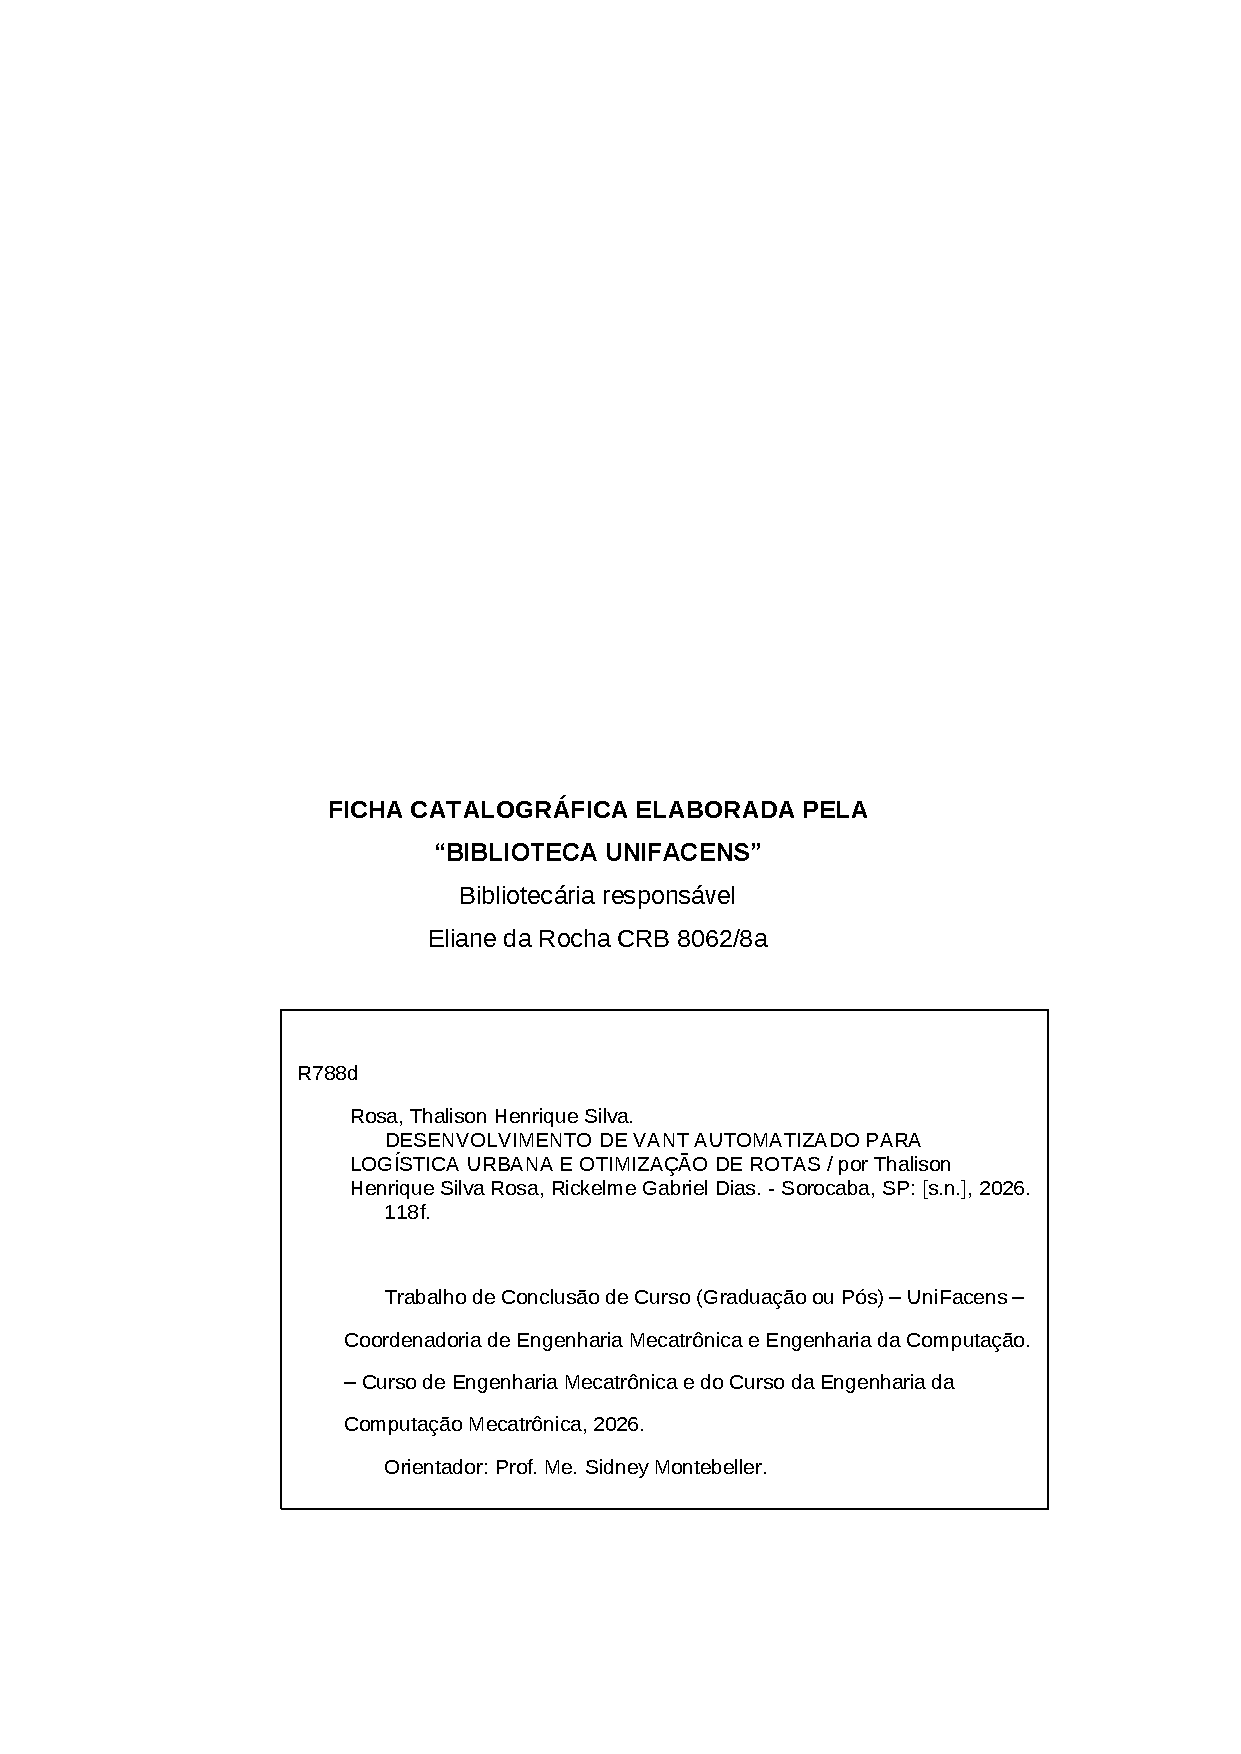
\includepdf[pages=1]{samples/FICHACATALOGRAFICA.pdf}
\end{fichacatalografica}
%\begin{errata}
    Elemento opcional da \citeonline[4.2.1.2]{NBR14724:2011}. Exemplo:

    \vspace{\onelineskip}

    FERRIGNO, C. R. A. \textbf{Tratamento de neoplasias ósseas apendiculares com
    reimplantação de enxerto ósseo autólogo autoclavado associado ao plasma
    rico em plaquetas}: estudo crítico na cirurgia de preservação de membro em
    cães. 2011. 128 f. Tese (Livre-Docência) - Faculdade de Medicina Veterinária e
    Zootecnia, Universidade de São Paulo, São Paulo, 2011.

    \begin{table}[htb]
        \center
        \footnotesize
        \begin{tabular}{|p{1.4cm}|p{1cm}|p{3cm}|p{3cm}|}
            \hline
            \textbf{Folha} & \textbf{Linha}  & \textbf{Onde se lê}  & \textbf{Leia-se}  \\
                \hline
                1 & 10 & auto-conclavo & autoconclavo\\
            \hline
        \end{tabular}
    \end{table}

\end{errata}
% ============================================================================
% FOLHA DE APROVACAO - UNIFACENS (Limpo e Corrigido)
% ============================================================================
\providecommand{\FapNomeUm}{RICKELME GABRIEL DIAS}
\providecommand{\FapNomeDois}{THALISON HENRIQUE SILVA ROSA}
\providecommand{\FapTituloLinhaUm}{DESENVOLVIMENTO DE VANT AUTOMATIZADO}
\providecommand{\FapTituloLinhaDois}{PARA LOGÍSTICA URBANA E OTIMIZAÇÃO DE ROTAS}
\providecommand{\FapOrientador}{Me. Sidney Montebeller}
\providecommand{\FapAvaliadorUm}{Dr. Denis Borg}
\providecommand{\FapAfiliacaoUm}{Centro Universitário Facens}
\providecommand{\FapAvaliadorDois}{Me. Marcos Fábio Jardini}
\providecommand{\FapAfiliacaoDois}{Centro Universitário Facens}
\providecommand{\FapAvaliadorTres}{Me. Sidney Montebeller}
\providecommand{\FapAfiliacaoTres}{Centro Universitário Facens}

\clearpage
\begingroup
  \thispagestyle{empty}
  \setlength{\parindent}{0pt}
  \setlength{\parskip}{0pt}
  \frenchspacing

  \newcommand{\FapCentro}[3]{%
    \node[anchor=base,inner sep=0pt,outer sep=0pt,text=black] at
      ([xshift=297.65bp,yshift=-#1bp]current page.north west)
      {{\fontsize{#2bp}{#2bp}\selectfont #3}};%
  }
  \newcommand{\FapLinhaAssinatura}[1]{%
    \draw[black,line width=0.58bp]
      ([xshift=180.95bp,yshift=-#1bp]current page.north west)--
      ([xshift=414.5bp,yshift=-#1bp]current page.north west);%
  }

  \begin{tikzpicture}[remember picture,overlay]
    % ------------------------------------------------------------------------
    % 1 - ALUNO(S): Arial 12, Maiúsculas (Um nome por linha)
    % ------------------------------------------------------------------------
    \FapCentro{78.00}{12}{\bfseries \FapNomeUm}
    \FapCentro{93.00}{12}{\bfseries \FapNomeDois}

    % ------------------------------------------------------------------------
    % 2 - TÍTULO DO TRABALHO: Arial 14, Maiúsculas
    % ------------------------------------------------------------------------
    \FapCentro{152.00}{14}{\bfseries \MakeUppercase{\FapTituloLinhaUm}}
    \FapCentro{170.00}{14}{\bfseries \MakeUppercase{\FapTituloLinhaDois}}

    % ------------------------------------------------------------------------
    % 3 - NATUREZA DO TRABALHO: Recuo de 8cm, Texto Justificado, Arial 11
    % ------------------------------------------------------------------------
    \node[anchor=north west,align=justify,text width=7.2cm] at ([xshift=311.95bp,yshift=-270bp]current page.north west) {
      \fontsize{11bp}{13bp}\selectfont
      Trabalho de conclusão de curso apresentado ao Centro Universitário Facens como exigência parcial para obtenção do certificado de conclusão do curso de Engenharia da Computação e Engenharia Mecatrônica.\\
      Orientador: \FapOrientador.
    };

    % ------------------------------------------------------------------------
    % 4 - BANCA EXAMINADORA
    % ------------------------------------------------------------------------
    \FapCentro{455.00}{14}{\bfseries BANCA EXAMINADORA}

    % ------------------------------------------------------------------------
    % 5 - ASSINATURAS DOS AVALIADORES
    % ------------------------------------------------------------------------
    % 1º Avaliador
    \FapLinhaAssinatura{505.00}
    \FapCentro{520.00}{11}{\FapAvaliadorUm}
    \FapCentro{535.00}{11}{\FapAfiliacaoUm}

    % 2º Avaliador
    \FapLinhaAssinatura{590.00}
    \FapCentro{605.00}{11}{\FapAvaliadorDois}
    \FapCentro{620.00}{11}{\FapAfiliacaoDois}

    % 3º Avaliador
    \FapLinhaAssinatura{675.00}
    \FapCentro{690.00}{11}{\FapAvaliadorTres}
    \FapCentro{705.00}{11}{\FapAfiliacaoTres}

  \end{tikzpicture}
  \null
\endgroup
\clearpage
% ============================================================================
% DEDICATÓRIA (Opcional)
% FONTE: Manual Facens MSGQ-21.01 REV.18
%
% REGRAS:
% - NÃO escrever a palavra "DEDICATÓRIA" na página
% - Fonte Arial 12pt, espaçamento 1,5, alinhado à DIREITA
% - Texto no final da página
% - Recomendável uma única dedicatória por trabalho
%   (se for em grupo e cada membro quiser a sua, uma por página)
% ============================================================================

\begin{dedicatoria}
    \vspace*{\fill} % Empurra o texto para o final da página

    \begin{flushright}
        \begin{minipage}{10cm}
            \begin{OnehalfSpace}
                Dedicamos este trabalho às nossas famílias e aos nossos amigos,
                pelo apoio, pela compreensão e pelo incentivo ao longo desta jornada.
                A todos que estiveram ao nosso lado e nos ajudaram a seguir em frente
                diante das dificuldades, dedicamos esta conquista.
            \end{OnehalfSpace}
        \end{minipage}
    \end{flushright}
\end{dedicatoria}

\begin{agradecimentos}
    Agradecemos às nossas famílias pelo apoio e pela compreensão durante o
    desenvolvimento deste trabalho. O incentivo de vocês foi fundamental para
    enfrentarmos as dificuldades e seguirmos com dedicação até esta etapa.

    Aos nossos amigos, agradecemos pela presença, pelas palavras de incentivo e
    pelo apoio ao longo desta jornada.

    Ao nosso orientador, professor Me. Sidney Montebeller, por todo apoio durante o desenvolvimento do trabalho.

    Agradecemos especialmente ao nosso colega Vinicius Silva, que participou ativamente
    da construção física do drone e nos ajudou a superar dificuldades práticas
    de montagem, em especial nas soldagens mais complexas. Sua disponibilidade
    e sua colaboração foram muito importantes para o desenvolvimento do protótipo.
\end{agradecimentos}

%\begin{epigrafe}
    \vspace*{\fill}
    
    \begin{flushright}
        \begin{minipage}{8cm}
            \begin{SingleSpace}
                ``Não vos amoldeis às estruturas deste mundo,
                mas transformai-vos pela renovação da mente,
                a fim de distinguir qual é a vontade de Deus:
                o que é bom, o que Lhe é agradável, o que é perfeito.``\\
                (Bíblia Sagrada, Romanos 12, 2)
            \end{SingleSpace}
        \end{minipage}
    \end{flushright}
\end{epigrafe}

\setlength{\absparsep}{18pt}
\begin{resumo}
\SingleSpacing
{\setlength{\parindent}{1.27cm}\par\noindent\hspace*{\parindent}Este trabalho apresenta o desenvolvimento de uma plataforma experimental de veículo aéreo não tripulado para investigar a integração entre controle de voo e planejamento de missões em ambiente controlado. A arquitetura combina um controlador de voo STM32F411, responsável pela aquisição de sensores, estimação de estados, controle LQG e funções de segurança, com um Raspberry Pi Zero W, responsável pelo planejamento de rotas e pela coordenação sequencial dos comandos de missão. A metodologia compreende modelagem, simulação no MATLAB/Simulink, desenvolvimento embarcado e ensaios de bancada e de voo. Os ensaios dos sensores forneceram dados para a caracterização do ruído de medição, e os testes do conjunto propulsor permitiram caracterizar o empuxo. No ensaio de voo real, observou-se estabilização de rolamento e arfagem; em voo livre, a deriva horizontal e de guinada durante a subida impediu que a referência de altitude fosse alcançada. A comunicação DroneLink foi avaliada pela UART entre o Raspberry Pi e o STM32 reais, com o veículo simulado no microcontrolador e os motores parados: durante os 60 segundos de observação do enlace, não foram registradas perdas nem erros de checksum, e a mediana da latência de ida e volta foi de 10,2 ms. No planejamento de rotas, foram avaliadas 280 instâncias com 3 a 30 pontos. O algoritmo genético obteve o ótimo global em 150 das 200 instâncias em que a solução ótima era conhecida e produziu rotas idênticas no computador pessoal e no Raspberry Pi nas três instâncias comparadas. Os resultados sustentam a viabilidade dos módulos desenvolvidos, enquanto a deriva observada em voo evidencia a necessidade de aperfeiçoar o posicionamento horizontal antes da validação física de missões completas.\par}

\noindent\textbf{Palavras-chave}: veículo aéreo não tripulado. quadricóptero. regulador linear quadrático gaussiano. sistemas embarcados. otimização de rotas.
\end{resumo}

\begin{resumo}[Abstract]
\begin{otherlanguage*}{english}
\SingleSpacing
{\setlength{\parindent}{1.27cm}\par\noindent\hspace*{\parindent}This work presents the development of an experimental unmanned aerial vehicle platform to investigate the integration of flight control and mission planning in a controlled environment. The architecture combines an STM32F411 flight controller, responsible for sensor acquisition, state estimation, LQG control and safety functions, with a Raspberry Pi Zero W, responsible for route planning and the sequential coordination of mission commands. The methodology comprises modelling, MATLAB/Simulink simulation, embedded development, and bench and flight experiments. Sensor experiments provided data for measurement noise characterization, while propulsion tests characterized thrust. The physical flight experiment showed roll and pitch stabilization; in free flight, horizontal and yaw drift during the climb prevented the altitude reference from being reached. DroneLink communication was evaluated over UART between the physical Raspberry Pi and STM32, with the vehicle simulated on the microcontroller and the motors stopped: no packet losses or checksum errors were recorded during the 60-second link observation period, and median round-trip latency was 10.2 ms. Route planning was evaluated on 280 instances with 3 to 30 points. The genetic algorithm found the global optimum in 150 of the 200 instances with a known optimal solution and produced identical routes on the personal computer and Raspberry Pi for the three compared instances. The results support the feasibility of the developed modules, while the drift observed in flight indicates that horizontal positioning requires further improvement before complete missions can be validated in physical flight.\par}

\noindent\textbf{Keywords}: unmanned aerial vehicle. quadrotor. linear quadratic Gaussian regulator. embedded systems. route optimization.
\end{otherlanguage*}
\end{resumo}


% --- LISTAS ---
\pdfbookmark[0]{\listfigurename}{lof}
\listoffigures*
\cleardoublepage
\pdfbookmark[0]{\listofquadrosname}{loq}
\listofquadros*
\cleardoublepage
\pdfbookmark[0]{\listtablename}{lot}
\listoftables*
\cleardoublepage
\begin{siglas}
    \item[AG] Algoritmo Genético
    \item[AM32] Firmware aberto para controladores eletrônicos de velocidade de motores sem escova
    \item[ANAC] Agência Nacional de Aviação Civil
    \item[BEC] \textit{Battery Eliminator Circuit}
    \item[BLDC] \textit{Brushless Direct Current}
    \item[CCW] \textit{Counter-Clockwise}
    \item[CMSIS] \textit{Cortex Microcontroller Software Interface Standard}
    \item[CRC] \textit{Cyclic Redundancy Check}
    \item[CW] \textit{Clockwise}
    \item[DECEA] Departamento de Controle do Espaço Aéreo
    \item[DMA] \textit{Direct Memory Access}
    \item[DShot] \textit{Digital Shot}
    \item[EKF] \textit{Extended Kalman Filter}
    \item[ESC] \textit{Electronic Speed Controller}
    \item[FPU] \textit{Floating-Point Unit}
    \item[GPIO] \textit{General-Purpose Input/Output}
    \item[HAL] \textit{Hardware Abstraction Layer}
    \item[HSE] \textit{High-Speed External}
    \item[I2C] \textit{Inter-Integrated Circuit}
    \item[IMU] \textit{Inertial Measurement Unit}
    \item[LiDAR] \textit{Light Detection and Ranging}
    \item[LQG] \textit{Linear Quadratic Gaussian}
    \item[LQI] \textit{Linear Quadratic Integral}
    \item[LQR] \textit{Linear Quadratic Regulator}
    \item[LTR] \textit{Loop Transfer Recovery}
    \item[MAE] \textit{Mean Absolute Error}
    \item[MAVLink] \textit{Micro Air Vehicle Link}
    \item[NED] \textit{North-East-Down}
    \item[OX] \textit{Order Crossover}
    \item[PWM] \textit{Pulse Width Modulation}
    \item[RAM] \textit{Random Access Memory}
    \item[RBAC] Regulamento Brasileiro da Aviação Civil
    \item[RMSE] \textit{Root Mean Square Error}
    \item[RTOS] \textit{Real-Time Operating System}
    \item[SH-2] \textit{Sensor Hub 2}
    \item[SHA] \textit{Secure Hash Algorithm}
    \item[SHTP] \textit{Sensor Hub Transport Protocol}
    \item[SPI] \textit{Serial Peripheral Interface}
    \item[SRAM] \textit{Static Random Access Memory}
    \item[STM32] Família de microcontroladores da STMicroelectronics
    \item[ToF] \textit{Time of Flight}
    \item[TSP] \textit{Travelling Salesman Problem}
    \item[UAM] \textit{Urban Air Mobility}
    \item[UART] \textit{Universal Asynchronous Receiver-Transmitter}
    \item[USB] \textit{Universal Serial Bus}
    \item[UTM] \textit{Unmanned Traffic Management}
    \item[VANT] Veículo Aéreo Não Tripulado
    \item[VTOL] \textit{Vertical Take-Off and Landing}
    \item[XML] \textit{Extensible Markup Language}
\end{siglas}

\clearpage
\begin{simbolos}
    \item[$m$, $M$] Massa total do quadricóptero, em quilogramas (kg)
    \item[$g$] Aceleração da gravidade, em metros por segundo ao quadrado (m/s$^2$)
    \item[$l$] Distância radial entre o centro do veículo e o motor, em metros (m)
    \item[$d$] Braço projetado do motor em relação ao eixo de rotação, em metros (m)
    \item[$K_t$] Coeficiente de empuxo do conjunto motor--hélice
    \item[$K_q$] Coeficiente de torque do conjunto motor--hélice
    \item[$T$] Empuxo total gerado pelos quatro rotores, em newtons (N)
    \item[$F_i$] Empuxo gerado pelo motor $i$, em newtons (N)
    \item[$\omega_i$] Velocidade angular do motor $i$, em radianos por segundo (rad/s)
    \item[$\omega_0$] Velocidade angular de equilíbrio dos motores em voo estacionário (rad/s)
    \item[$\tau_\phi,\tau_\theta,\tau_\psi$] Momentos de rolamento, arfagem e guinada
    \item[$\phi,\theta,\psi$] Ângulos de Euler de rolamento, arfagem e guinada
    \item[$p,q,r$] Velocidades angulares do corpo em torno dos eixos $x_B$, $y_B$ e $z_B$
    \item[$I_{xx},I_{yy},I_{zz}$] Momentos principais de inércia do veículo
    \item[$\mathbf{R}$] Matriz de rotação entre o referencial do corpo e o referencial inercial
    \item[$\mathbf{A},\mathbf{B},\mathbf{C},\mathbf{D}$] Matrizes de estados, de entrada, de saída e de transmissão direta do modelo linearizado
    \item[$\mathbf{A}_d,\mathbf{B}_d$] Matrizes de estados e de entrada do modelo discretizado
    \item[$T_s$] Período de amostragem, em segundos (s)
    \item[$\mathbf{Q}$] Matriz de ponderação dos estados no LQR
    \item[$\mathbf{R}_{\mathrm{lqr}}$] Matriz de ponderação do esforço de controle no LQR
    \item[$\mathbf{K}$] Matriz de ganhos de realimentação de estados
    \item[$\mathbf{S}$] Solução da equação algébrica de Riccati do LQR
    \item[$J$] Funcional de custo quadrático
    \item[$\mathbf{L}$] Matriz de ganhos do filtro de Kalman
    \item[$\mathbf{P}$] Matriz de covariância do erro de estimação
    \item[$\mathbf{Q}_w$] Matriz de covariância do ruído de processo
    \item[$\mathbf{R}_v$] Matriz de covariância do ruído de medição
    \item[$\mathbf{w},\mathbf{v}$] Ruídos de processo e de medição
    \item[$\mathbf{x}$] Vetor de estados do modelo
    \item[$\hat{\mathbf{x}}$] Vetor de estados estimado
    \item[$\mathbf{u}$] Vetor de entradas de controle
    \item[$\mathbf{y}$] Vetor de saídas medidas pelos sensores
    \item[$N$] Número de pontos a visitar na rota
    \item[$P_0$] Ponto de partida e de retorno da rota
    \item[$C(\pi)$] Custo (comprimento) do circuito associado à ordem de visita $\pi$
    \item[$d(a,b)$] Distância euclidiana entre os pontos $a$ e $b$
\end{simbolos}

\clearpage

% --- SUMÁRIO ---
\pdfbookmark[0]{\contentsname}{toc}
\tableofcontents*
\cleardoublepage

% ============================================================================
% ELEMENTOS TEXTUAIS (CORPO DO TRABALHO)
% ============================================================================

\textual                        
\pagestyle{cabecalhopaginaimpar}

\chapter{INTRODUÇÃO}\label{cap:introducao}

Veículos Aéreos Não Tripulados (VANTs) são empregados em inspeção, mapeamento, monitoramento e aplicações logísticas. No contexto de entregas urbanas, o planejamento de rotas e a segurança operacional são questões centrais, pois a missão precisa respeitar restrições de energia, tempo, ambiente e regulamentação \cite{otto2018,rinaldi2024}. No Brasil, operações de aeronaves não tripuladas de uso civil estão sujeitas aos requisitos gerais da Agência Nacional de Aviação Civil (ANAC) e aos procedimentos de acesso ao espaço aéreo definidos pelo Departamento de Controle do Espaço Aéreo (DECEA) \cite{anac2026,decea2026}. Este trabalho não propõe operação comercial ou urbana em espaço aéreo aberto; utiliza o cenário logístico como motivação para o desenvolvimento de uma plataforma experimental em ambiente controlado.

Um quadricóptero autônomo combina problemas de naturezas distintas. O planejamento de missão requer selecionar uma sequência de pontos que reduza o custo de deslocamento, problema relacionado ao Problema do Caixeiro Viajante. A estabilidade da aeronave, por sua vez, exige controle em tempo real de um sistema subatuado, não linear e sujeito a perturbações \cite{beard2012,quan2017}. A integração dessas funções demanda uma arquitetura em que o planejamento não comprometa as funções críticas de estimação, controle e segurança.

Essa integração é relevante porque muitos estudos tratam separadamente o planejamento de rotas, o controle de atitude e a comunicação embarcada. Em um protótipo físico, entretanto, essas partes compartilham restrições de processamento, temporização, sensores, alimentação elétrica e tolerância a falhas. Uma rota calculada corretamente perde valor se não puder ser traduzida em comandos seguros, e um controlador estável em simulação precisa ser confrontado com atrasos, saturações e ruídos presentes no sistema real.

Outra motivação do trabalho é a reprodutibilidade de uma arquitetura experimental de baixo custo relativo. Plataformas abertas, como STM32, Raspberry Pi, FreeRTOS e MAVLink, permitem documentação detalhada das interfaces e dos procedimentos de teste. Essa escolha favorece a análise acadêmica do sistema, pois torna possível registrar versões de hardware, bibliotecas, ferramentas, parâmetros de controle e critérios de avaliação.

O objetivo geral deste trabalho é desenvolver uma plataforma experimental de VANT para investigar a integração entre planejamento de rotas e controle de voo autônomo. A estratégia de controle adotada é o Regulador Linear Quadrático Gaussiano (LQG), que combina um Regulador Linear Quadrático (LQR), projetado a partir da linearização do modelo do quadricóptero em torno da condição de voo estacionário, com um filtro de Kalman para a estimação dos estados. A escolha permite explicitar o compromisso entre desvios de estado e esforço de atuação por meio das matrizes de ponderação do problema de controle ótimo \cite{jafari2010,okyere2019}.

Os objetivos específicos são: modelar a cinemática e a dinâmica do quadricóptero; construir e simular o controlador LQG; implementar a arquitetura embarcada em STM32F411 com FreeRTOS; integrar a comunicação entre o controlador de voo e o Raspberry Pi Zero W; estruturar um Algoritmo Genético para planejamento de rotas; e definir ensaios de bancada, simulação e voo controlado para avaliar o sistema. A validação em voo só foi realizada depois das verificações elétricas, de comunicação e de segurança descritas neste trabalho.

A arquitetura proposta separa a camada de voo da camada de missão. O STM32F411 executa leitura de sensores, estimação, controle LQG, mistura de motores, comando DShot e \textit{failsafes}. O Raspberry Pi Zero W realiza funções de missão, rede, telemetria e registro. A comunicação entre essas camadas é especificada como DroneLink 1.0, protocolo próprio do projeto baseado em UART e enquadramento MAVLink 2 \cite{koubaa2019,mavlinkguide}. O Raspberry Pi envia objetivos de missão e telemetria de alto nível, enquanto o STM32 permanece responsável pelas ações críticas de controle e segurança. Para a estimativa de atitude, o projeto adota um módulo da família BNO08X; o MTF-01 fornece medições de fluxo óptico e distância utilizadas nos testes internos \cite{bno08xdatasheet,micoair2024}.

Como resultado, o trabalho apresenta uma base para experimentos de autonomia em ambiente controlado, com separação clara entre missão e controle de voo. Também foram produzidos artefatos de apoio à continuidade do projeto, incluindo modelo matemático, critérios de sintonia do controlador LQG, especificação de comunicação, configuração dos periféricos e sequência de ensaios. Esses resultados não substituem certificação, validação operacional externa ou atendimento a requisitos regulatórios de voo em espaço aéreo aberto.

O método combina pesquisa bibliográfica, modelagem, simulação, desenvolvimento de \textit{firmware} e experimentação progressiva. As evidências de desempenho são tratadas apenas a partir de simulações, ensaios de bancada e registros experimentais definidos no procedimento metodológico.

Além desta introdução, o Capítulo~\ref{cap_revisao} apresenta os fundamentos de quadricópteros, controle LQG, planejamento de rotas e sistemas embarcados. O Capítulo~\ref{cap:metodologia} descreve os materiais, o ambiente de desenvolvimento, os procedimentos e os critérios de avaliação. O Capítulo~\ref{cap:resultados} apresenta e discute os resultados dos sensores, das simulações, do voo, da comunicação e do planejamento de rotas. O Capítulo~\ref{cap:conclusao} reúne as considerações finais e os trabalhos futuros.

\clearpage
\chapter{REVISÃO BIBLIOGRÁFICA}\label{cap_revisao}

Este capítulo apresenta os fundamentos teóricos que sustentam o desenvolvimento do sistema proposto. Inicialmente, contextualiza-se a evolução histórica dos VANTs e suas classificações. Em seguida, descreve-se o princípio de funcionamento do quadricóptero e sua modelagem matemática. Abordam-se a representação em espaço de estados e o controle por Regulador Linear Quadrático Gaussiano (LQG). Por fim, discutem-se os algoritmos de otimização de rotas e a arquitetura de \textit{hardware} embarcado empregada.

% ================================================================
\section{VEÍCULOS AÉREOS NÃO TRIPULADOS: HISTÓRICO E CLASSIFICAÇÃO}
% ================================================================

Os Veículos Aéreos Não Tripulados (VANTs), conhecidos popularmente como \textit{drones}, tiveram seus primeiros registros em meados do século XIX. Em 1849, o exército austríaco utilizou balões não tripulados carregando explosivos para bombardear a cidade de Veneza, marcando uma das primeiras aplicações militares de aeronaves sem piloto na história \cite{mori2020, zaloga2008}. Esses veículos evoluíram continuamente ao longo dos conflitos globais; na Primeira Guerra Mundial, destaca-se o torpedo aéreo Hewitt-Sperry, guiado por giroscópio, que demonstrou a viabilidade do voo autônomo controlado por instrumentos \cite{newcome2004}. Em 1935, a Marinha Real britânica desenvolveu o \textit{DH.82B Queen Bee}, um avião rádio-controlado para treinamento de artilharia antiaérea, cuja denominação inspirou o termo \textit{drone} --- ``zangão'' em inglês --- como uma alusão à sua ``abelha-rainha'' \cite{zaloga2008, newcome2004}.

A partir da década de 1960, VANTs passaram a ser empregados sistematicamente em missões de reconhecimento e vigilância, e nas décadas seguintes consolidaram-se como ferramentas estratégicas em operações militares de larga escala \cite{ayamga2021}. A transição para aplicações civis acelerou-se na década de 2010 com o surgimento de plataformas multirrotoras comerciais acessíveis, que democratizaram o acesso à tecnologia e impulsionaram o crescimento do mercado global de VANTs \cite{sivakumar2021, kapustina2021}.

\begin{figure}[H]
    \centering
    \caption{Comparativo visual de VANTs: (a) Asa Fixa, (b) Multicóptero e (c) VTOL Híbrido.}
    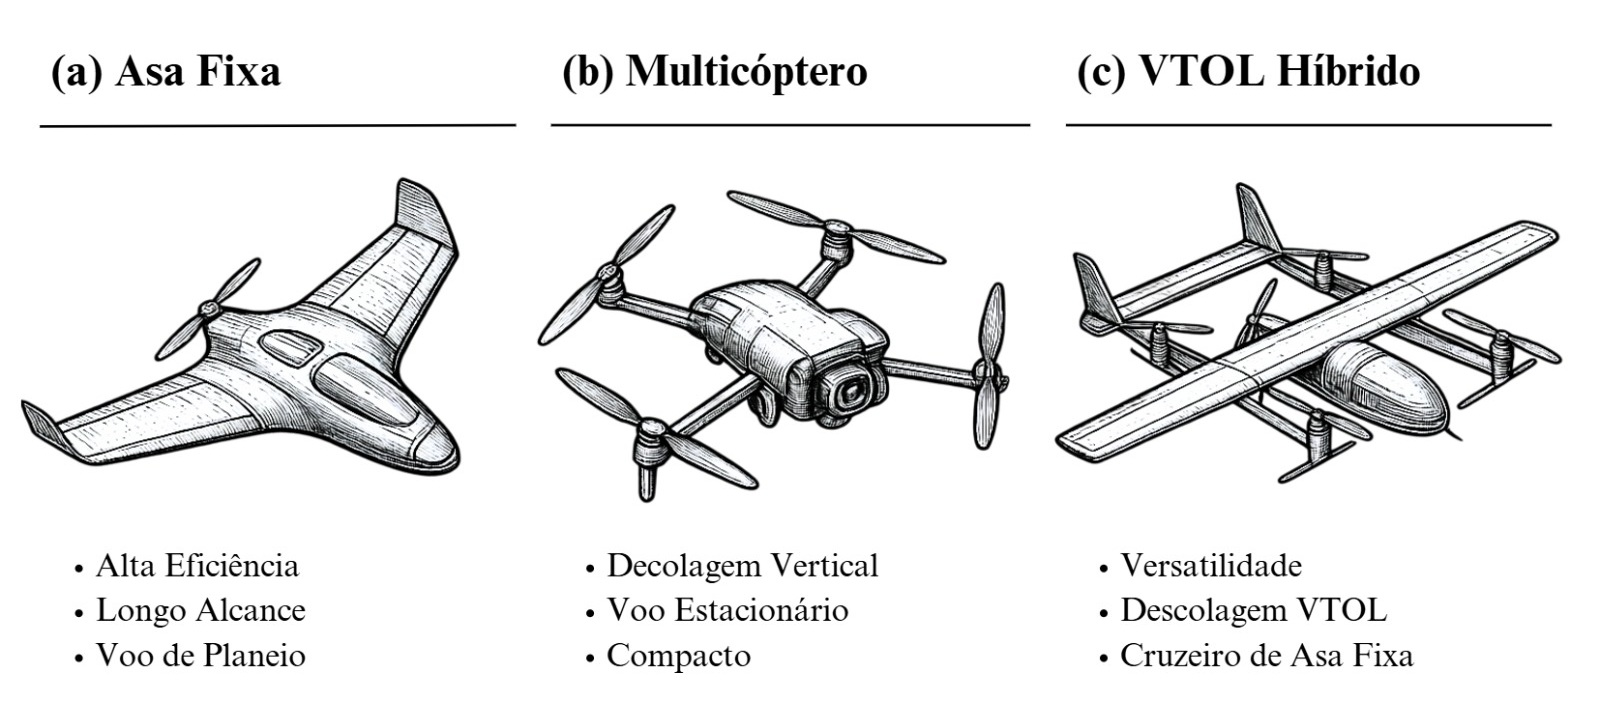
\includegraphics[width=0.8\textwidth]{images/introducao/AsaFixaMulticopteroVTOLHibrido.jpg}
    \label{fig:AsaFixaMulticopteroVTOLHibrido}
    \par\vspace{0.2cm}
    \centering\footnotesize Fonte: elaborado pelos autores (2026).
\end{figure}

Os VANTs são classificados principalmente pela sua configuração aerodinâmica, conforme ilustrado na Figura \ref{fig:AsaFixaMulticopteroVTOLHibrido}. Os modelos de Asa Fixa (a) destacam-se pela alta eficiência energética e longo alcance, sendo ideais para voos de planeio e missões de mapeamento extenso. Em contrapartida, os Multicópteros (b) oferecem a capacidade de voo estacionário e decolagem vertical em espaços compactos, embora possuam menor autonomia comparativa \cite{mohsan2023}. Por fim, os \textit{Vertical Take-Off and Landing} Híbridos (VTOLs) (c) combinam a versatilidade da decolagem vertical com a eficiência do voo de cruzeiro de asa fixa \cite{guebsi2024}.

A evolução desses veículos permitiu sua adoção em setores estratégicos. Na agricultura de precisão, VANTs possibilitam o monitoramento em tempo real de lavouras e aplicação localizada de insumos \cite{barbosajunior2024}. No setor da saúde, a tecnologia é empregada para mitigar gargalos logísticos na entrega de suprimentos vitais, como hemoderivados e medicamentos essenciais, em regiões de infraestrutura comprometida ou zonas de conflito \cite{ahmad2026}. Já na logística empresarial, o foco reside na etapa de \textit{last-mile delivery} (entrega de última milha), em que as rotas, a energia disponível e as restrições operacionais influenciam custo e nível de serviço \cite{rinaldi2024,otto2018}.

No Brasil, a Agência Nacional de Aviação Civil (ANAC) estabelece requisitos gerais para aeronaves não tripuladas de uso civil por meio do RBAC nº 100 \cite{anac2026}. O Departamento de Controle do Espaço Aéreo (DECEA), por sua vez, define procedimentos de acesso ao espaço aéreo brasileiro para sistemas de aeronaves remotamente pilotadas, incluindo critérios de solicitação, coordenação e autorização de voo \cite{decea2026}. Conceitos como \textit{Unmanned Traffic Management} (UTM) e \textit{Urban Air Mobility} (UAM) aparecem nesse contexto como temas relacionados à coordenação de operações não tripuladas e mobilidade aérea urbana, mas não substituem os requisitos normativos aplicáveis ao tipo de operação efetivamente realizado.

% ================================================================
\section{PRINCÍPIO DE FUNCIONAMENTO DE UM QUADRICÓPTERO}
% ================================================================

O quadricóptero integra a categoria de multicópteros de asas rotativas. Esse tipo de VANT possui quatro propulsores que, ao operarem em sincronia, geram o empuxo resultante necessário para realizar os movimentos de subida e descida. Adicionalmente, ao controlar a velocidade angular de cada motor individualmente, torna-se possível realizar as demais movimentações de atitude e translação. A disposição dos motores e hélices é comumente dividida nas configurações ``X'' (\textit{cross}) e ``+'' (\textit{plus}), conforme ilustrado na Figura~\ref{fig:quadrotor_flight_configurations} \cite{idrissi2022}.

\begin{figure}[H]
    \centering
    \caption{Configurações de voo de quadricópteros: (a) Plus e (b) Cross.}
    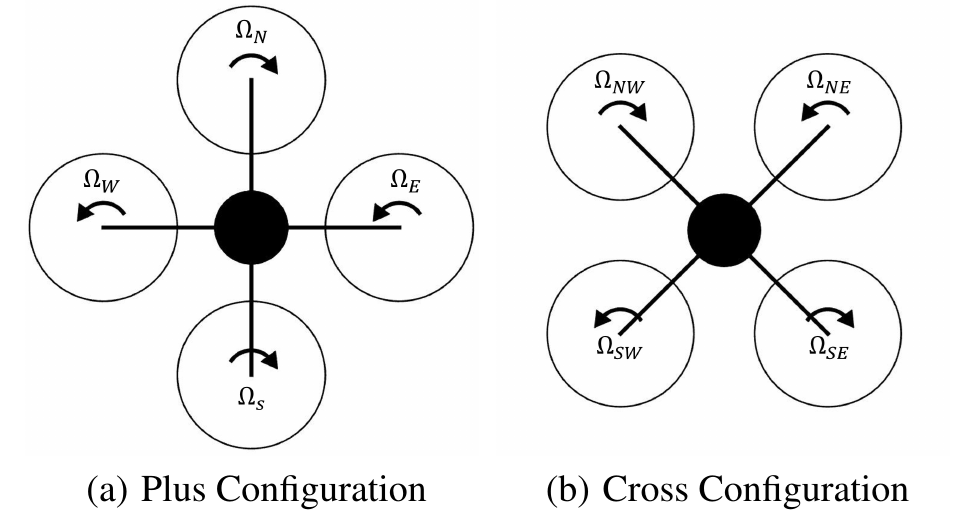
\includegraphics[width=0.8\textwidth]{images/referencial_teorico/quadrotor_flight_configurations.png}
    \label{fig:quadrotor_flight_configurations}
    \par\vspace{0.2cm}
    \centering\footnotesize Fonte: \citeonline{niemiec2016}.
\end{figure}

Em ambas as configurações, rotores adjacentes giram em sentidos opostos --- um par no sentido horário (\textit{clockwise} --- CW) e outro no sentido anti-horário (\textit{counter-clockwise} --- CCW). Essa disposição é fundamental para cancelar o torque reativo resultante da rotação das hélices, permitindo o controle do ângulo de guinada (\textit{yaw}) do veículo \cite{quan2017}. De acordo com \citeonline{niemiec2016}, nas condições analisadas pelos autores, a configuração ``X'' apresentou autoridade de controle em arfagem (\textit{pitch}) e rolamento (\textit{roll}) até aproximadamente 30\% maior que a configuração ``+''. Por essa razão, a configuração ``X'' é recorrente em plataformas comerciais e acadêmicas, sendo também a empregada neste projeto.

A movimentação do quadricóptero é governada por quatro modos de controle distintos, denominados coletivo, arfagem, rolamento e guinada, conforme descrito a seguir \cite{beard2012}:

\begin{alineastcc}
    \item \textbf{controle coletivo} ($\Omega_0$): todos os quatro motores aumentam ou diminuem a velocidade angular simultaneamente. Próximo ao voo nivelado e em uma plataforma simétrica, esse modo altera principalmente o empuxo total ($T$), com efeito direto sobre a aceleração vertical (Figura~\ref{fig:collective_control});
    \item \textbf{controle de arfagem} ($\Omega_P$): os rotores dianteiros aceleram enquanto os traseiros desaceleram (ou vice-versa), produzindo um momento em torno do eixo lateral ($y$) que inclina o veículo para frente ou para trás. Essa inclinação redireciona parte do vetor de empuxo para a horizontal, gerando aceleração longitudinal (Figura~\ref{fig:pitch_control});
    \item \textbf{controle de rolamento} ($\Omega_R$): de forma análoga ao controle de arfagem, os rotores do lado esquerdo aceleram enquanto os do lado direito desaceleram (ou vice-versa), produzindo um momento em torno do eixo longitudinal ($x$) que resulta em deslocamento lateral (Figura~\ref{fig:roll_control});
    \item \textbf{controle de guinada} ($\Omega_Y$): os rotores que giram no sentido horário (CW) aceleram enquanto os que giram no sentido anti-horário (CCW) desaceleram (ou vice-versa). Esse diferencial de torque reativo produz um momento em torno do eixo vertical ($z$), alterando a orientação do veículo (Figura~\ref{fig:yaw_control}).
\end{alineastcc}

\begin{figure}[H]
    \centering
    \caption{Controle coletivo ($\Omega_0$): variação uniforme da velocidade em todos os motores para controle de altitude.}
    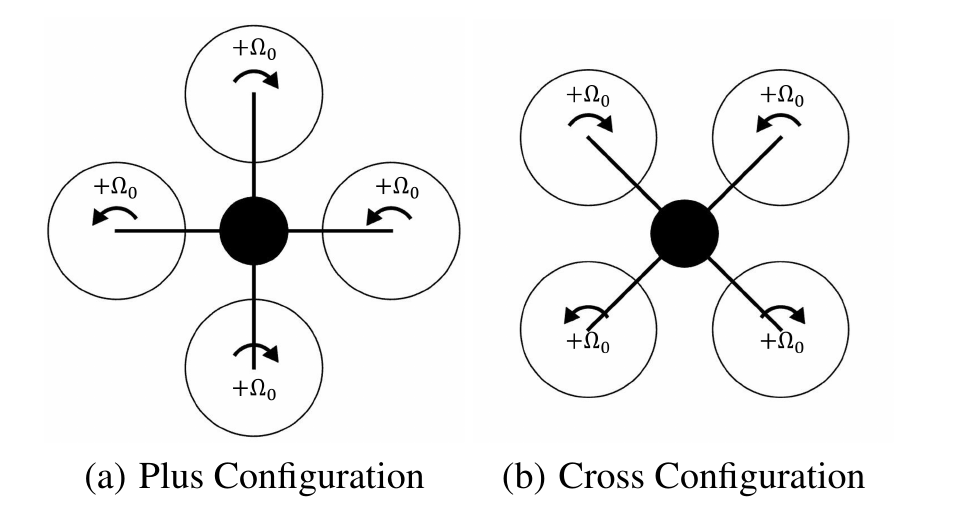
\includegraphics[width=0.8\textwidth]{images/referencial_teorico/collective_control.png}
    \label{fig:collective_control}
    \par\vspace{0.2cm}
    \centering\footnotesize Fonte: \citeonline{niemiec2016}.
\end{figure}

\begin{figure}[H]
    \centering
    \caption{Controle de arfagem ($\Omega_P$): diferencial de velocidade entre rotores dianteiros e traseiros para inclinação longitudinal.}
    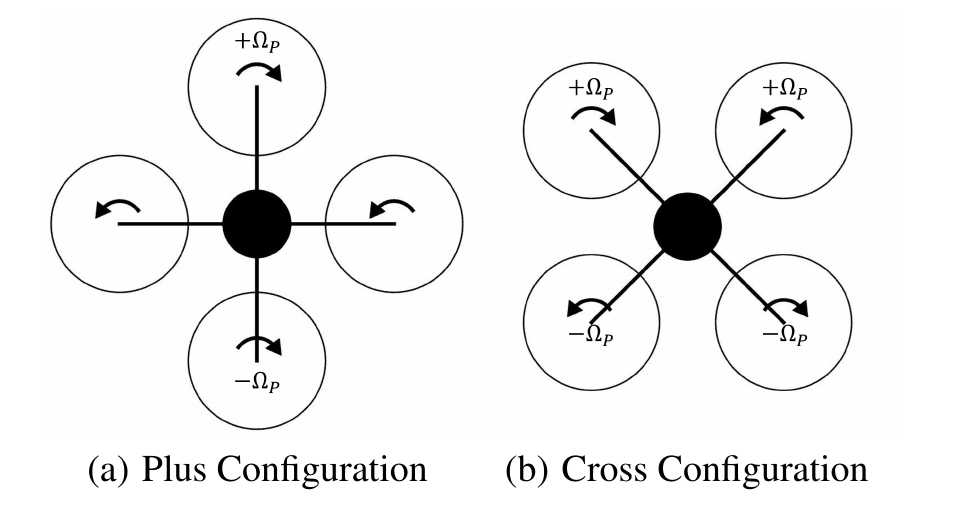
\includegraphics[width=0.8\textwidth]{images/referencial_teorico/pitch_control.png}
    \label{fig:pitch_control}
    \par\vspace{0.2cm}
    \centering\footnotesize Fonte: \citeonline{niemiec2016}.
\end{figure}

\begin{figure}[H]
    \centering
    \caption{Controle de rolamento ($\Omega_R$): diferencial de velocidade entre rotores esquerdo e direito para inclinação lateral.}
    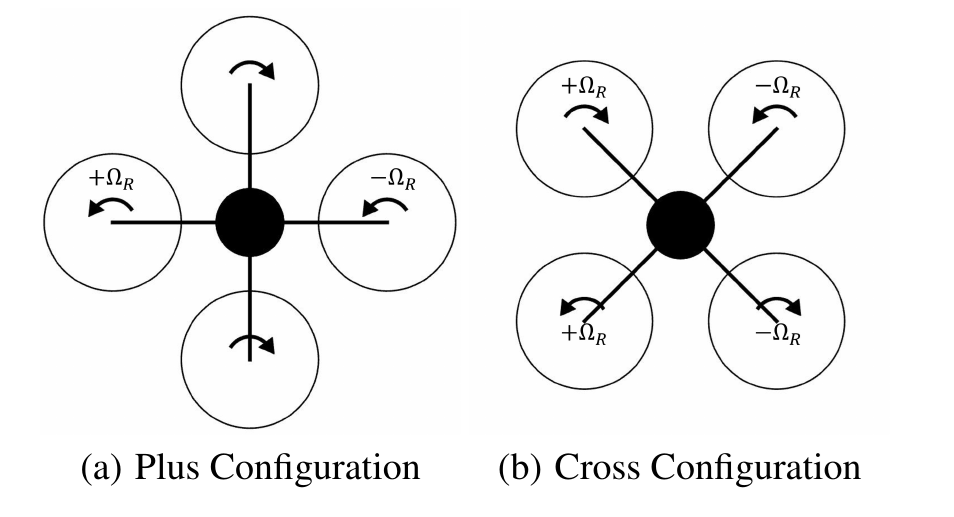
\includegraphics[width=0.8\textwidth]{images/referencial_teorico/roll_control.png}
    \label{fig:roll_control}
    \par\vspace{0.2cm}
    \centering\footnotesize Fonte: \citeonline{niemiec2016}.
\end{figure}

\begin{figure}[H]
    \centering
    \caption{Controle de guinada ($\Omega_Y$): diferencial de torque reativo entre rotores CW e CCW para rotação em torno do eixo vertical.}
    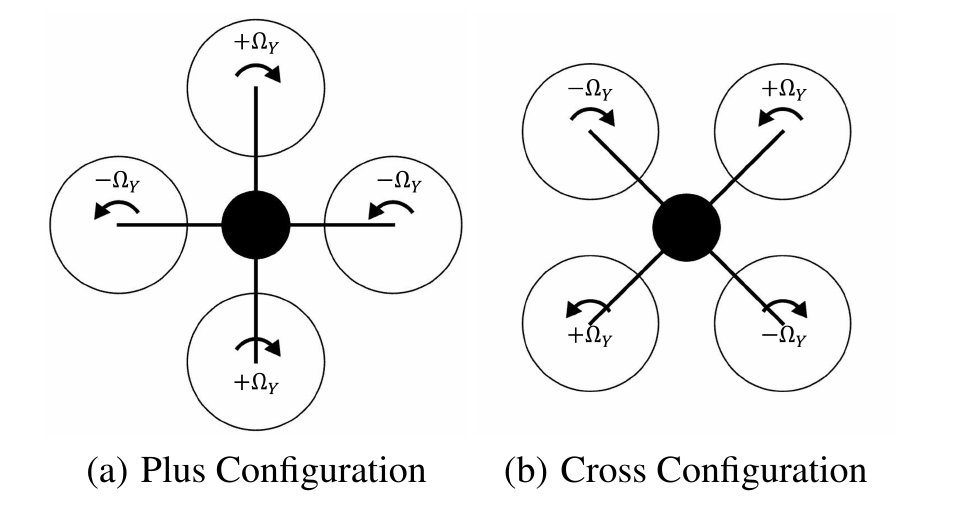
\includegraphics[width=0.8\textwidth]{images/referencial_teorico/yaw_control.png}
    \label{fig:yaw_control}
    \par\vspace{0.2cm}
    \centering\footnotesize Fonte: \citeonline{niemiec2016}.
\end{figure}

Essa decomposição dos movimentos é uma idealização útil próxima ao equilíbrio, sob hipóteses de simetria e pequenas inclinações. Conforme observado por \citeonline{idrissi2022}, essa estrutura evidencia que o quadricóptero é um sistema \textit{subatuado}: com apenas quatro entradas de controle, buscam-se controlar seis graus de liberdade --- três de translação ($x$, $y$, $z$) e três de rotação ($\phi$, $\theta$, $\psi$). Essa característica impõe restrições ao controle simultâneo de todas as variáveis e motiva a formulação em espaço de estados empregada pelo LQR, discutida na Seção~\ref{sec:controle}.

% ================================================================
\section{MODELAGEM MATEMÁTICA DO QUADRICÓPTERO}\label{sec:modelagem}
% ================================================================

A modelagem matemática de um quadricóptero consiste em descrever formalmente as relações entre as forças geradas pelos motores e o movimento resultante do veículo. Essa etapa é fundamental para o projeto de controladores, pois fornece as equações diferenciais que governam a planta a ser controlada. Nesta seção, seguem-se as formulações apresentadas por \citeonline{quan2017} e \citeonline{beard2012}, amplamente adotadas na literatura de VANTs multirrotores.

% ----------------------------------------------------------------
\subsection{Referenciais e ângulos de Euler}\label{subsec:referenciais}
% ----------------------------------------------------------------

Para descrever o movimento de um corpo rígido no espaço tridimensional, faz-se necessário definir dois sistemas de coordenadas: o referencial inercial (fixo ao solo) e o referencial do corpo (fixo ao veículo). O referencial inercial, denotado por $\mathcal{W} = \{x_W, y_W, z_W\}$, adota a convenção NED (\textit{North-East-Down}), na qual $x_W$ aponta para o norte, $y_W$ aponta para o leste e $z_W$ aponta para baixo. O referencial do corpo, denotado por $\mathcal{B} = \{x_B, y_B, z_B\}$, adota a convenção frente--direita--baixo: $x_B$ aponta para a frente do veículo, $y_B$ para a direita e $z_B$ para baixo \cite{beard2012}.

\begin{figure}[H]
    \centering
    \caption{Representação dos referenciais inercial ($\mathcal{W}$) e do corpo ($\mathcal{B}$).}
    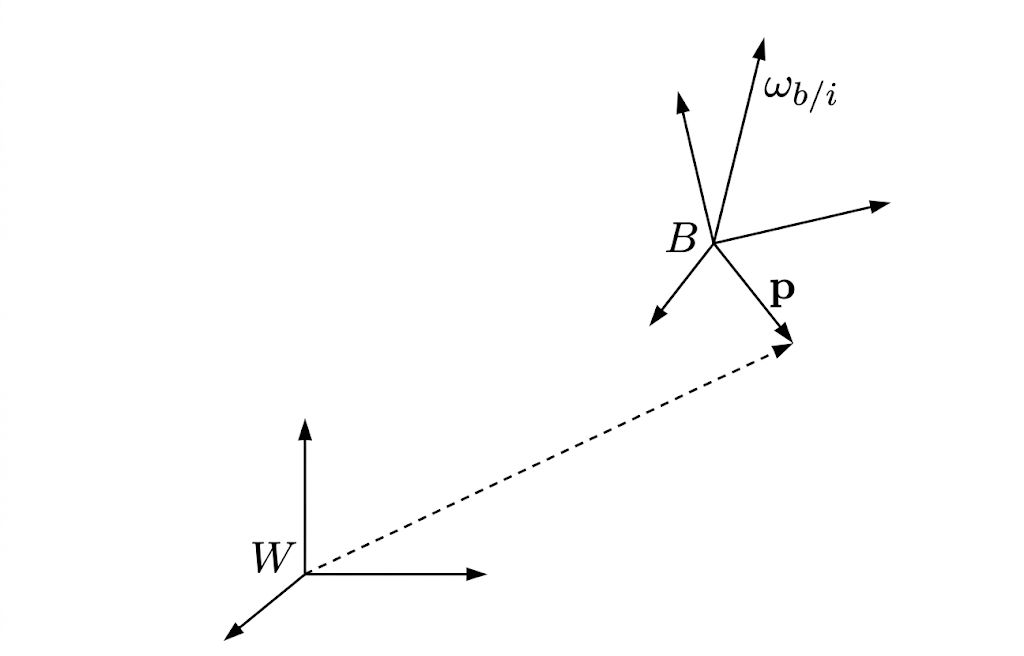
\includegraphics[width=0.6\textwidth]{images/referencial_teorico/Ref_Inercial_Corpo.jpg}
    \label{fig:referenciais_euler}
    \par\vspace{0.2cm}
    \centering\footnotesize Fonte: adaptado de \citeonline{beard2012}.
\end{figure}

A Figura~\ref{fig:referenciais_euler} representa genericamente o referencial inercial $\mathcal{W}$, o referencial do corpo $\mathcal{B}$, o vetor de posição entre eles e a velocidade angular do corpo em relação ao referencial inercial. O símbolo vetorial $\mathbf{p}$ indicado na imagem representa posição; ele não deve ser confundido com a variável escalar $p$ usada no modelo para a velocidade angular de rolamento. As direções específicas da convenção NED e dos eixos frente--direita--baixo são definidas no texto, pois a figura não identifica nominalmente cada eixo.

A orientação do referencial do corpo em relação ao referencial inercial é descrita pelos três ângulos de Euler: rolamento ($\phi$), arfagem ($\theta$) e guinada ($\psi$). A transformação entre os dois referenciais é realizada pela matriz de rotação $\mathbf{R}$, obtida pela composição de três rotações elementares na sequência ZYX \cite{quan2017}:

\begin{equation}\label{eq:rotacao}
\mathbf{R} = \mathbf{R}_z(\psi)\,\mathbf{R}_y(\theta)\,\mathbf{R}_x(\phi)
\end{equation}

\noindent resultando em:

\begin{equation}\label{eq:matriz_rotacao}
\mathbf{R} = \begin{bmatrix}
c\psi\, c\theta & c\psi\, s\theta\, s\phi - s\psi\, c\phi & c\psi\, s\theta\, c\phi + s\psi\, s\phi \\
s\psi\, c\theta & s\psi\, s\theta\, s\phi + c\psi\, c\phi & s\psi\, s\theta\, c\phi - c\psi\, s\phi \\
-s\theta & c\theta\, s\phi & c\theta\, c\phi
\end{bmatrix}
\end{equation}

\noindent onde $c(\cdot)$ e $s(\cdot)$ representam, respectivamente, cosseno e seno.

A relação entre as velocidades angulares medidas no referencial do corpo ($p$, $q$, $r$) e as taxas de variação dos ângulos de Euler ($\dot{\phi}$, $\dot{\theta}$, $\dot{\psi}$) é dada pela relação cinemática \cite{beard2012}:

\begin{equation}\label{eq:euler_rates}
\begin{bmatrix} \dot{\phi} \\ \dot{\theta} \\ \dot{\psi} \end{bmatrix} = \begin{bmatrix}
1 & s\phi\, t\theta & c\phi\, t\theta \\
0 & c\phi & -s\phi \\
0 & s\phi / c\theta & c\phi / c\theta
\end{bmatrix}
\begin{bmatrix} p \\ q \\ r \end{bmatrix}
\end{equation}

\noindent onde $t(\cdot)$ representa a tangente. Essa relação apresenta uma singularidade em $\theta = \pm 90^\circ$, conhecida como \textit{gimbal lock}. O envelope operacional adotado para o projeto deve permanecer afastado dessa singularidade; valores como $|\theta| < 15^\circ$ representam uma escolha de projeto a ser sustentada pela análise da planta não linear, e não um limite universal de validade do LQR \cite{quan2017}.

% ----------------------------------------------------------------
\subsection{Cinemática do quadricóptero}\label{subsec:cinematica}
% ----------------------------------------------------------------

A cinemática descreve a geometria do movimento sem considerar as forças que o causam. O estado completo do quadricóptero é definido por 12 variáveis agrupadas no vetor de estado \cite{beard2012}:

\begin{equation}\label{eq:vetor_estado}
\mathbf{x} = \left[ \begin{array}{cccccccccccc} 
x & y & z & \phi & \theta & \psi & \dot{x} & \dot{y} & \dot{z} & p & q & r 
\end{array} \right]^T
\end{equation}

\noindent onde $(x, y, z)$ é a posição no referencial inercial, $(\phi, \theta, \psi)$ são os ângulos de Euler, $(\dot{x}, \dot{y}, \dot{z})$ são as velocidades lineares no referencial inercial, e $(p, q, r)$ são as velocidades angulares no referencial do corpo.

As equações cinemáticas translacionais são triviais:
\begin{equation}\label{eq:cine_trans}
\dot{x} = v_x, \quad \dot{y} = v_y, \quad \dot{z} = v_z
\end{equation}

\noindent enquanto as equações cinemáticas rotacionais são dadas pela Equação~\eqref{eq:euler_rates}. Juntas, essas seis equações cinemáticas formam a primeira metade do modelo de 12 estados.

% ----------------------------------------------------------------
\subsection{Dinâmica do quadricóptero}\label{subsec:dinamica}
% ----------------------------------------------------------------

A dinâmica do quadricóptero é governada pelas leis de Newton para translação e pelas equações de Euler para rotação. Cada motor $i$ gera uma força de empuxo ($F_i$) e um torque de reação aerodinâmica ($\tau_{M,i}$) proporcionais ao quadrado de sua velocidade angular ($\omega_i$) \cite{quan2017}:

\begin{equation}\label{eq:empuxo_torque_motor}
F_i = K_t \, \omega_i^2 \quad \text{e} \quad \tau_{M,i} = K_q \, \omega_i^2
\end{equation}

\noindent onde $K_t$ é o coeficiente de empuxo (em $\mathrm{N\cdot s^2/rad^2}$) e $K_q$ é o coeficiente de torque (em $\mathrm{N\cdot m\cdot s^2/rad^2}$). O empuxo estático total ($T$) do veículo é dado pela soma dos empuxos individuais:

\begin{equation}\label{eq:empuxo_total}
T = \sum_{i=1}^{4} F_i = K_t \sum_{i=1}^{4} \omega_i^2
\end{equation}

Os torques atuantes nos três eixos do corpo são expressos em função dos esforços individuais e da geometria do veículo. Para a configuração em ``X'', define-se $d$ como a distância projetada do eixo do motor aos eixos principais de rotação (rolamento e arfagem). Em um chassi simétrico, sendo $l$ a distância radial do centro de massa até o motor, tem-se $d = l/\sqrt{2}$. 

A relação entre os esforços individuais e os esforços totais (empuxo $T$ e torques de rolamento $\tau_\phi$, arfagem $\tau_\theta$ e guinada $\tau_\psi$) é descrita por uma matriz de alocação de controle \cite{quan2017}. Definindo a constante $c = K_q$, a matriz (conhecida na literatura como \textit{motor mixing matrix}) assume a seguinte forma:

\begin{equation}\label{eq:mixing}
\begin{bmatrix} T \\ \tau_\phi \\ \tau_\theta \\ \tau_\psi \end{bmatrix}
= \begin{bmatrix}
1 & 1 & 1 & 1 \\
d & -d & -d & d \\
d & d & -d & -d \\
c & -c & c & -c
\end{bmatrix}
\begin{bmatrix} F_1 \\ F_2 \\ F_3 \\ F_4 \end{bmatrix}
\end{equation}

\noindent A correta aplicação desta matriz de mistura exige a definição prévia da disposição física dos motores, dos respectivos sentidos de rotação (horário ou anti-horário), da associação com os canais dos ESCs (\textit{Electronic Speed Controllers}) e da convenção de sinais dos momentos. De forma generalizada, para um motor localizado na coordenada $(x_i,y_i,0)$ do referencial do corpo e gerando empuxo vertical, as contribuições espaciais de torque são $\tau_{\phi,i} = y_i F_i$ e $\tau_{\theta,i} = -x_i F_i$. Por fim, a implementação prática desta alocação via protocolo DShot requer a caracterização experimental para mapear a relação não linear entre o comando digital, a tensão de alimentação e os esforços efetivamente gerados pelo conjunto motor-hélice.

Aplicando-se a Segunda Lei de Newton no referencial inercial NED, com empuxo no sentido $-z_B$ e $\mathbf{R}$ como transformação do corpo para o referencial inercial, obtém-se $m\ddot{\mathbf{r}}=mg\mathbf{e}_3-T\mathbf{R}\mathbf{e}_3$. Portanto, as equações dinâmicas translacionais são \cite{beard2012}:

\begin{equation}\label{eq:din_x}
m\ddot{x} = -T\,(c\psi\, s\theta\, c\phi + s\psi\, s\phi)
\end{equation}
\begin{equation}\label{eq:din_y}
m\ddot{y} = -T\,(s\psi\, s\theta\, c\phi - c\psi\, s\phi)
\end{equation}
\begin{equation}\label{eq:din_z}
m\ddot{z} = mg - T\, c\theta\, c\phi
\end{equation}

\noindent e as equações dinâmicas rotacionais:

\begin{equation}\label{eq:din_p}
I_{xx}\,\dot{p} = \tau_\phi - (I_{zz} - I_{yy})\,q\,r
\end{equation}
\begin{equation}\label{eq:din_q}
I_{yy}\,\dot{q} = \tau_\theta - (I_{xx} - I_{zz})\,p\,r
\end{equation}
\begin{equation}\label{eq:din_r}
I_{zz}\,\dot{r} = \tau_\psi - (I_{yy} - I_{xx})\,p\,q
\end{equation}

\noindent onde $m$ é a massa total do veículo, $g$ é a aceleração gravitacional e $I_{xx}$, $I_{yy}$, $I_{zz}$ são os momentos de inércia principais. As equações assumem corpo rígido, tensor de inércia diagonal, eixos principais de inércia alinhados aos eixos do corpo e efeitos aerodinâmicos adicionais desprezados. Os termos $(I_{zz} - I_{yy})\,qr$ e análogos representam o acoplamento inercial entre os eixos; momentos giroscópicos específicos dos rotores não são incluídos explicitamente nessa formulação.

O modelo de 12 estados reúne a cinemática angular da Equação~\eqref{eq:euler_rates}, a cinemática translacional da Equação~\eqref{eq:cine_trans}, a dinâmica translacional das Equações~\eqref{eq:din_x}--\eqref{eq:din_z} e a dinâmica rotacional das Equações~\eqref{eq:din_p}--\eqref{eq:din_r}. As Equações~\eqref{eq:empuxo_motor}--\eqref{eq:mixing} descrevem relações algébricas de geração e alocação dos esforços. Esse modelo não linear é utilizado diretamente na simulação da planta no Simulink, enquanto uma versão linearizada é empregada no projeto do controlador, conforme discutido na seção seguinte.

% ================================================================
\section{CONTROLE DE VOO POR REGULADOR LINEAR QUADRÁTICO GAUSSIANO}\label{sec:controle}
% ================================================================

O controle de voo de um quadricóptero tem como objetivo levar o estado do veículo a uma referência com estabilidade, respeitando os limites dos atuadores e lidando com sensores ruidosos que não medem todos os estados. Nesta seção, apresentam-se: (i) a linearização do modelo não linear pela matriz Jacobiana (série de Taylor de primeira ordem); (ii) o Regulador Linear Quadrático (LQR), que calcula a realimentação ótima de estados; (iii) o filtro de Kalman, que estima os estados a partir de medições ruidosas; e (iv) a combinação dos dois no controlador Linear Quadrático Gaussiano (LQG) \cite{athans1971,anderson1990}. O LQR e o filtro de Kalman são métodos baseados em critérios de otimalidade, e não técnicas empíricas de sintonia de ganhos.

% ----------------------------------------------------------------
\subsection{Representação em espaço de estados e linearização}\label{subsec:espaco_estados}
% ----------------------------------------------------------------

O modelo não linear do quadricóptero, derivado na Seção~\ref{sec:modelagem}, pode ser expresso na forma geral de espaço de estados \cite{ogata2010}:

\begin{equation}\label{eq:ss_geral}
\dot{\mathbf{x}}(t) = f(\mathbf{x}(t),\, \mathbf{u}(t)), \qquad \mathbf{y}(t) = h(\mathbf{x}(t),\, \mathbf{u}(t)),
\end{equation}

\noindent onde $\mathbf{x} \in \mathbb{R}^{12}$ reúne posição, atitude, velocidades linear e angular, $\mathbf{u} = [\omega_1, \omega_2, \omega_3, \omega_4]^T$ é o vetor de entrada e $\mathbf{y}$ é o vetor de saídas medidas pelos sensores.

\subsubsection{Ponto de equilíbrio}

Um ponto de equilíbrio $(\mathbf{x}_0,\mathbf{u}_0)$ satisfaz $f(\mathbf{x}_0,\mathbf{u}_0)=\mathbf{0}$. Neste trabalho adota-se o voo estacionário (\textit{hover}), no qual $\phi_0=\theta_0=0$, todas as velocidades são nulas e $\mathbf{u}_0=[\omega_0,\omega_0,\omega_0,\omega_0]^T$, onde $w_0$ é a velocidade angular de equilíbrio \cite{quan2017}.

\subsubsection{Linearização por série de Taylor}

Definem-se as variáveis de desvio $\delta\mathbf{x}=\mathbf{x}-\mathbf{x}_0$ e $\delta\mathbf{u}=\mathbf{u}-\mathbf{u}_0$. Expandindo $f$ em série de Taylor em torno de $(\mathbf{x}_0,\mathbf{u}_0)$ e retendo apenas os termos de primeira ordem:

\begin{equation}\label{eq:taylor}
f(\mathbf{x},\mathbf{u}) = \underbrace{f(\mathbf{x}_0,\mathbf{u}_0)}_{=\,\mathbf{0}} + \left.\frac{\partial f}{\partial \mathbf{x}}\right|_{0}\delta\mathbf{x} + \left.\frac{\partial f}{\partial \mathbf{u}}\right|_{0}\delta\mathbf{u} + \mathbf{r}(\delta\mathbf{x},\delta\mathbf{u}),
\end{equation}

\noindent em que o resto satisfaz $\|\mathbf{r}\| = O\!\left(\|\delta\mathbf{x}\|^2+\|\delta\mathbf{u}\|^2\right)$ e é desprezado. As matrizes do modelo linear são as Jacobianas de $f$ e de $h$ avaliadas no ponto de equilíbrio:

\begin{equation}\label{eq:jacobianas}
\mathbf{A}=\left.\frac{\partial f}{\partial \mathbf{x}}\right|_{0},\quad
\mathbf{B}=\left.\frac{\partial f}{\partial \mathbf{u}}\right|_{0},\quad
\mathbf{C}=\left.\frac{\partial h}{\partial \mathbf{x}}\right|_{0},\quad
\mathbf{D}=\left.\frac{\partial h}{\partial \mathbf{u}}\right|_{0},
\end{equation}

\noindent isto é, $A_{ij}=\partial f_i/\partial x_j$ e $B_{ij}=\partial f_i/\partial u_j$. O modelo linearizado é

\begin{equation}\label{eq:ss_linear}
\delta\dot{\mathbf{x}} = \mathbf{A}\,\delta\mathbf{x} + \mathbf{B}\,\delta\mathbf{u}, \qquad
\delta\mathbf{y} = \mathbf{C}\,\delta\mathbf{x} + \mathbf{D}\,\delta\mathbf{u}.
\end{equation}

\noindent A mesma construção equivale à aproximação de ângulos pequenos ($\sin\alpha \approx \alpha$, $\cos\alpha \approx 1$) \cite{quan2017}. As Jacobianas podem ser obtidas analiticamente ou por cálculo simbólico/numérico, devendo-se conferir o resultado por simulação do modelo não linear.

\subsubsection{Estrutura do modelo linearizado em \textit{hover}}

Desprezando-se os termos de acoplamento giroscópico (de segunda ordem nos desvios) e adotando a convenção NED com guinada nominal $\psi_0=0$, o modelo se desacopla nos seguintes canais:

\begin{align}
\delta\ddot{z} &= -\frac{\delta T}{m}, &
\delta\ddot{\psi} &= \frac{\delta\tau_\psi}{I_{zz}}, \label{eq:canal_zpsi}\\
\delta\ddot{x} &= -g\,\delta\theta, &
\delta\ddot{\theta} &= \frac{\delta\tau_\theta}{I_{yy}}, \label{eq:canal_x}\\
\delta\ddot{y} &= g\,\delta\phi, &
\delta\ddot{\phi} &= \frac{\delta\tau_\phi}{I_{xx}}. \label{eq:canal_y}
\end{align}

Essas equações mostram uma propriedade fundamental do quadricóptero: a translação horizontal é controlada indiretamente pelos ângulos de atitude (o sistema é subatuado). Para uma guinada nominal qualquer, os acoplamentos horizontais dependem de $\psi_0$; assim, o controle de posição deve transformar erros para o referencial apropriado ou atualizar o modelo linearizado conforme a orientação da aeronave.

\subsubsection{Validade e discretização}

O modelo linear só é válido na vizinhança do ponto de operação, pois o resto $\mathbf{r}$ cresce quadraticamente com o desvio. Pelo método indireto de Lyapunov, se a malha fechada linearizada tem todos os autovalores com parte real negativa, o equilíbrio da planta não linear é localmente assintoticamente estável \cite{khalil2002}; essa garantia é local, e a região de atração deve ser verificada por simulação com o modelo não linear. Para implementação em computador embarcado, o modelo é discretizado com período de amostragem $T_s$ e retentor de ordem zero:

\begin{equation}\label{eq:discretizacao}
\mathbf{A}_d=e^{\mathbf{A}T_s},\qquad
\mathbf{B}_d=\int_0^{T_s}e^{\mathbf{A}\tau}\,d\tau\,\mathbf{B},
\end{equation}

\noindent resultando em $\delta\mathbf{x}_{k+1}=\mathbf{A}_d\delta\mathbf{x}_k+\mathbf{B}_d\delta\mathbf{u}_k$ \cite{franklin1998}.

% ----------------------------------------------------------------
\subsection{Regulador Linear Quadrático (LQR)}\label{subsec:lqr}
% ----------------------------------------------------------------

Considerando o sistema linear invariante no tempo da Equação~\eqref{eq:ss_linear}, o LQR contínuo procura a entrada de desvio $\delta\mathbf{u}$ que minimiza o funcional de custo quadrático

\begin{equation}\label{eq:custo_lqr}
J = \int_0^{\infty}\left(\delta\mathbf{x}^{T}\mathbf{Q}\,\delta\mathbf{x}+\delta\mathbf{u}^{T}\mathbf{R}_{\mathrm{lqr}}\,\delta\mathbf{u}\right)dt,
\end{equation}

\noindent em que $\mathbf{Q}=\mathbf{Q}^T\succeq0$ penaliza os desvios de estado e $\mathbf{R}_{\mathrm{lqr}}=\mathbf{R}_{\mathrm{lqr}}^T\succ0$ penaliza o esforço de controle. A solução assume a forma de realimentação de estados

\begin{equation}\label{eq:lei_lqr}
\delta\mathbf{u}=-\mathbf{K}\,\delta\mathbf{x},\qquad \mathbf{K}=\mathbf{R}_{\mathrm{lqr}}^{-1}\mathbf{B}^{T}\mathbf{S},
\end{equation}

\noindent em que $\mathbf{S}=\mathbf{S}^T\succeq 0$ é a solução da equação algébrica de Riccati

\begin{equation}\label{eq:riccati_lqr}
\mathbf{A}^{T}\mathbf{S}+\mathbf{S}\mathbf{A}-\mathbf{S}\mathbf{B}\mathbf{R}_{\mathrm{lqr}}^{-1}\mathbf{B}^{T}\mathbf{S}+\mathbf{Q}=\mathbf{0},
\end{equation}

\noindent quando não há termo cruzado no custo \cite{ogata2010,anderson1990,mathworkslqr}. Para a solução estabilizante usual, requerem-se $(\mathbf{A},\mathbf{B})$ estabilizável e $(\mathbf{Q}^{1/2},\mathbf{A})$ detectável; controlabilidade completa é condição mais forte que estabilizabilidade \cite{anderson1990}. Para a versão discreta, o ganho deve ser calculado com a equação de Riccati discreta (por exemplo, \texttt{dlqr}), usando $\mathbf{A}_d$, $\mathbf{B}_d$ e o mesmo período de amostragem da implementação.

\subsubsection{Escolha das ponderações}

As matrizes $\mathbf{Q}$ e $\mathbf{R}_{\mathrm{lqr}}$ expressam a prioridade relativa entre reduzir erros de posição, velocidade, atitude e taxa angular, e limitar os comandos de empuxo e torque. Os valores dessas matrizes são escolhidos pelo projetista e precisam ser avaliados com critérios verificáveis, como tempo de acomodação, sobressinal, esforço de controle e margens de estabilidade \cite{mathworkslqr}.

\subsubsection{Lei de controle completa e limitações}

Para estabilizar um ponto de equilíbrio, a lei completa é $\mathbf{u}=\mathbf{u}_0-\mathbf{K}(\mathbf{x}-\mathbf{x}_0)$, com $\mathbf{u}_0=[mg,0,0,0]^T$ no voo estacionário nivelado. Para referência móvel, é necessário definir uma entrada nominal compatível com $\dot{\mathbf{x}}_{ref}=f(\mathbf{x}_{ref},\mathbf{u}_{ref})$; apenas somar $mg$ não descreve os esforços exigidos por acelerações da trajetória. Saturações de motor, limites de inclinação e limites de taxa devem ser especificados e verificados, pois a saturação aplicada após o LQR não garante, por si só, o respeito ao envelope operacional. Caso seja necessária integração do erro para rejeitar perturbações constantes, a extensão deve ser denominada LQI ou LQRi e descrita com o estado aumentado correspondente \cite{srivastava2024}.

Estudos com quadricópteros utilizam o LQR após linearização em torno do voo estacionário e avaliam resposta temporal, saturação e robustez do ganho obtido \cite{jafari2010,okyere2019}. O LQR, porém, supõe que todo o vetor $\delta\mathbf{x}$ esteja disponível para realimentação, o que não ocorre na prática: sensores medem apenas parte dos estados e com ruído. Isso motiva o uso de um estimador de estados.

% ----------------------------------------------------------------
\subsection{Filtro de Kalman}\label{subsec:kalman}
% ----------------------------------------------------------------

O filtro de Kalman fornece a estimativa $\delta\hat{\mathbf{x}}$ de variância mínima do estado a partir das entradas aplicadas e das medições ruidosas \cite{kalman1960,kalmanbucy1961}. Acrescentam-se ao modelo da Equação~\eqref{eq:ss_linear} um ruído de processo $\mathbf{w}$, que representa perturbações e erros de modelagem, e um ruído de medição $\mathbf{v}$:

\begin{equation}\label{eq:ss_ruido}
\delta\dot{\mathbf{x}} = \mathbf{A}\,\delta\mathbf{x} + \mathbf{B}\,\delta\mathbf{u} + \mathbf{G}\,\mathbf{w},\qquad
\delta\mathbf{y} = \mathbf{C}\,\delta\mathbf{x} + \mathbf{v},
\end{equation}

\noindent com $\mathbf{w}$ e $\mathbf{v}$ ruídos brancos gaussianos, de média nula, não correlacionados entre si, com intensidades $\mathbf{Q}_w\succeq0$ e $\mathbf{R}_v\succ0$. Aqui, $\mathbf{C}$ vem da Jacobiana de $h$ (Equação~\eqref{eq:jacobianas}) e depende dos sensores efetivamente disponíveis no protótipo.

\subsubsection{Estrutura do estimador}

O estimador tem a estrutura de um observador de estados, com um termo de correção proporcional à inovação (diferença entre a medição e a saída prevista):

\begin{equation}\label{eq:observador}
\delta\dot{\hat{\mathbf{x}}} = \mathbf{A}\,\delta\hat{\mathbf{x}} + \mathbf{B}\,\delta\mathbf{u} + \mathbf{L}\left(\delta\mathbf{y}-\mathbf{C}\,\delta\hat{\mathbf{x}}\right).
\end{equation}

\noindent No regime permanente, o ganho ótimo é $\mathbf{L}=\mathbf{P}\mathbf{C}^{T}\mathbf{R}_v^{-1}$, em que $\mathbf{P}=\mathbf{P}^T\succeq0$ é a covariância do erro de estimação, solução da equação algébrica de Riccati do filtro:

\begin{equation}\label{eq:riccati_kalman}
\mathbf{A}\mathbf{P}+\mathbf{P}\mathbf{A}^{T}-\mathbf{P}\mathbf{C}^{T}\mathbf{R}_v^{-1}\mathbf{C}\mathbf{P}+\mathbf{G}\mathbf{Q}_w\mathbf{G}^{T}=\mathbf{0}.
\end{equation}

\noindent A Equação~\eqref{eq:riccati_kalman} é a dual da Equação~\eqref{eq:riccati_lqr}: o ganho $\mathbf{L}$ pode ser calculado como um LQR para o par $(\mathbf{A}^T,\mathbf{C}^T)$, com $\mathbf{G}\mathbf{Q}_w\mathbf{G}^T$ no papel de $\mathbf{Q}$ e $\mathbf{R}_v$ no papel de $\mathbf{R}_{\mathrm{lqr}}$ \cite{anderson1990,simon2006}. Requerem-se $(\mathbf{A},\mathbf{C})$ detectável e $(\mathbf{A},\mathbf{G}\mathbf{Q}_w^{1/2})$ estabilizável; para estimar todos os estados, $(\mathbf{A},\mathbf{C})$ deve ser observável, o que impõe exigências sobre o conjunto de sensores.

\subsubsection{Forma discreta}

Na implementação digital, com $\mathbf{Q}_d$ e $\mathbf{R}_d$ as covariâncias discretizadas, o filtro opera em dois passos a cada período $T_s$:

\begin{align}
\text{Predição:}\quad
\delta\hat{\mathbf{x}}_{k|k-1} &= \mathbf{A}_d\,\delta\hat{\mathbf{x}}_{k-1|k-1}+\mathbf{B}_d\,\delta\mathbf{u}_{k-1}, \label{eq:kf_pred_x}\\
\mathbf{P}_{k|k-1} &= \mathbf{A}_d\,\mathbf{P}_{k-1|k-1}\,\mathbf{A}_d^{T}+\mathbf{Q}_d, \label{eq:kf_pred_P}\\[4pt]
\text{Atualização:}\quad
\mathbf{L}_k &= \mathbf{P}_{k|k-1}\mathbf{C}^{T}\left(\mathbf{C}\mathbf{P}_{k|k-1}\mathbf{C}^{T}+\mathbf{R}_d\right)^{-1}, \label{eq:kf_ganho}\\
\delta\hat{\mathbf{x}}_{k|k} &= \delta\hat{\mathbf{x}}_{k|k-1}+\mathbf{L}_k\left(\delta\mathbf{y}_k-\mathbf{C}\,\delta\hat{\mathbf{x}}_{k|k-1}\right), \label{eq:kf_upd_x}\\
\mathbf{P}_{k|k} &= \left(\mathbf{I}-\mathbf{L}_k\mathbf{C}\right)\mathbf{P}_{k|k-1}. \label{eq:kf_upd_P}
\end{align}

\noindent O filtro é ótimo (variância mínima) para sistemas lineares com ruídos gaussianos; para ruídos não gaussianos, é o melhor estimador linear \cite{simon2006,welch2006}. As covariâncias $\mathbf{Q}_w$ e $\mathbf{R}_v$ devem ser obtidas, sempre que possível, das especificações e de ensaios dos sensores (variância do ruído medida com o veículo parado), e não apenas ajustadas por tentativa. Se o veículo operar longe do \textit{hover}, a linearização única deixa de representar a planta, e uma alternativa é o filtro de Kalman estendido (EKF), que relineariza o modelo a cada passo em torno da estimativa corrente \cite{simon2006,welch2006}.

% ----------------------------------------------------------------
\subsection{Regulador Linear Quadrático Gaussiano (LQG)}\label{subsec:lqg}
% ----------------------------------------------------------------

O LQG resulta da combinação do LQR (Seção~\ref{subsec:lqr}) com o filtro de Kalman (Seção~\ref{subsec:kalman}): o ganho $\mathbf{K}$ é calculado como se o estado fosse conhecido, e a lei de controle é aplicada sobre a estimativa $\delta\hat{\mathbf{x}}$ fornecida pelo filtro \cite{athans1971,anderson1990}:

\begin{equation}\label{eq:lqg_lei}
\delta\mathbf{u}=-\mathbf{K}\,\delta\hat{\mathbf{x}}.
\end{equation}

\noindent Para ruídos gaussianos, essa combinação minimiza o valor esperado do custo quadrático,

\begin{equation}\label{eq:custo_lqg}
J_{\mathrm{LQG}}=\lim_{T\to\infty}\frac{1}{T}\,\mathbb{E}\left\{\int_0^{T}\left(\delta\mathbf{x}^{T}\mathbf{Q}\,\delta\mathbf{x}+\delta\mathbf{u}^{T}\mathbf{R}_{\mathrm{lqr}}\,\delta\mathbf{u}\right)dt\right\}.
\end{equation}

\subsubsection{Princípio da separação}

Definindo o erro de estimação $\mathbf{e}=\delta\mathbf{x}-\delta\hat{\mathbf{x}}$, a dinâmica em malha fechada é

\begin{equation}\label{eq:separacao}
\begin{bmatrix}\delta\dot{\mathbf{x}}\\ \dot{\mathbf{e}}\end{bmatrix}
=
\begin{bmatrix}\mathbf{A}-\mathbf{B}\mathbf{K} & \mathbf{B}\mathbf{K}\\ \mathbf{0} & \mathbf{A}-\mathbf{L}\mathbf{C}\end{bmatrix}
\begin{bmatrix}\delta\mathbf{x}\\ \mathbf{e}\end{bmatrix}
+
\begin{bmatrix}\mathbf{G}\mathbf{w}\\ \mathbf{G}\mathbf{w}-\mathbf{L}\mathbf{v}\end{bmatrix}.
\end{equation}

\noindent Como a matriz é triangular em blocos, os autovalores da malha fechada são a união dos autovalores de $\mathbf{A}-\mathbf{B}\mathbf{K}$ (regulador) e de $\mathbf{A}-\mathbf{L}\mathbf{C}$ (estimador). Esse é o princípio da separação: $\mathbf{K}$ e $\mathbf{L}$ podem ser projetados de forma independente, e a estabilidade nominal da malha fechada está garantida se ambos forem estabilizantes \cite{athans1971,anderson1990}.

\subsubsection{Compensador resultante}

Substituindo a Equação~\eqref{eq:lqg_lei} na Equação~\eqref{eq:observador}, o controlador LQG é um compensador dinâmico de mesma ordem da planta, com entrada $\delta\mathbf{y}$ e saída $\delta\mathbf{u}$:

\begin{equation}\label{eq:compensador}
\delta\dot{\hat{\mathbf{x}}}=\left(\mathbf{A}-\mathbf{B}\mathbf{K}-\mathbf{L}\mathbf{C}\right)\delta\hat{\mathbf{x}}+\mathbf{L}\,\delta\mathbf{y},\qquad
\delta\mathbf{u}=-\mathbf{K}\,\delta\hat{\mathbf{x}}.
\end{equation}

\noindent Na planta real, os comandos enviados aos motores são $\mathbf{u}=\mathbf{u}_0+\delta\mathbf{u}$ e as medições são convertidas em desvios por $\delta\mathbf{y}=\mathbf{y}-\mathbf{y}_0$. Como a entrada $\delta\mathbf{u}$ usada no filtro deve ser a efetivamente aplicada, no caso de saturação deve-se alimentar o estimador com o comando saturado, para evitar divergência entre a estimativa e o estado real.

\subsubsection{Limitações e verificação}

O princípio da separação garante a estabilidade nominal, mas não a robustez: o LQG não herda as margens de estabilidade garantidas do LQR com realimentação de estados completa, e podem ocorrer margens arbitrariamente pequenas \cite{doyle1978}. Por isso, as margens de ganho e fase devem ser verificadas na malha aberta cortada na entrada da planta, e pode-se recorrer à recuperação da malha de transferência (LTR) para aproximar o desempenho do LQR \cite{doylestein1979,skogestad2005}. Como no caso do LQR, o resultado deve ser validado em simulação com o modelo não linear, com parâmetros medidos do veículo, atrasos, quantização e ruído reais dos sensores, pois massa, inércias, empuxo e dinâmica dos motores influenciam a resposta real \cite{jafari2010,okyere2019}.

% Otimização de rotas: TSP, AG, métodos exatos e heurísticas de referência
% ============================================================================
% REFERENCIAL TEÓRICO — Otimização de rotas (TSP, AG, métodos exatos e
% heurísticas de referência). Chamado em partes/textuais/referencial_teorico.tex.
% ============================================================================

% ================================================================
\section{OTIMIZAÇÃO DE ROTAS}\label{sec:otimizacao}
% ================================================================

A eficiência de um sistema de entregas por VANT depende não apenas do controle de voo, mas da ordem estratégica em que os pontos são visitados. Nesta seção, formaliza-se o problema de otimização sob a ótica do Problema do Caixeiro Viajante e justifica-se o uso de Algoritmos Genéticos para lidar com a complexidade inerente ao cenário logístico; por fim, apresentam-se os métodos exatos e as heurísticas usados como referência de comparação.

% ----------------------------------------------------------------
\subsection{O Problema do Caixeiro Viajante e sua Complexidade}\label{subsec:tsp}
% ----------------------------------------------------------------

O planejamento de visitas a pontos de entrega pode ser modelado a partir do Problema do Caixeiro Viajante (TSP --- \textit{Travelling Salesman Problem}), cujo objetivo clássico é determinar o percurso de menor custo que visite um conjunto de pontos exatamente uma vez, retornando à origem. Considerando um ponto de partida $P_0$ e $N$ pontos a visitar, uma rota é uma permutação $\pi = (\pi_1, \dots, \pi_N)$, e seu custo é o comprimento do circuito:

\begin{equation}\label{eq:rotas_custo}
    C(\pi) = d(P_0, P_{\pi_1}) + \sum_{i=1}^{N-1} d(P_{\pi_i}, P_{\pi_{i+1}}) + d(P_{\pi_N}, P_0),
\end{equation}

\noindent em que, para pontos tridimensionais, $d(a,b)$ é a distância euclidiana

\begin{equation}\label{eq:rotas_distancia}
    d(a,b) = \sqrt{(x_a-x_b)^2 + (y_a-y_b)^2 + (z_a-z_b)^2}.
\end{equation}

Segundo \citeonline{cormen2012}, o TSP é classificado como NP-difícil: não se conhece algoritmo de tempo polinomial que resolva exatamente todas as suas instâncias, e sua dificuldade é expressa por reduções entre problemas. Com $n = N+1$ vértices, existem $N!$ permutações e, identificando os percursos reversos, $(n-1)!/2$ circuitos distintos para $n \geq 3$. A rota de menor custo entre todas é o \textbf{ótimo global}; uma rota que nenhuma modificação de uma vizinhança previamente definida consegue melhorar é um \textbf{ótimo local}, que pode ser bem pior que o global, e cuja quantidade cresce com o número de pontos \cite{johnson1997}.

A busca pela rota mais curta não é apenas uma questão geométrica. Em operações logísticas, a rota afeta o tempo de missão e o cumprimento de prazos de entrega \cite{rinaldi2024}; em um multirrotor, a distância percorrida também determina boa parte do consumo de energia, e a autonomia é limitada pela bateria \cite{wu2024}. Assim, encurtar a rota reduz ao mesmo tempo o tempo de voo e a energia necessária para a missão.

Dado o crescimento do espaço de busca em instâncias maiores e a possibilidade de soluções locais, métodos exatos podem se tornar computacionalmente onerosos. Algoritmos Genéticos (AGs) oferecem uma alternativa estocástica para explorar soluções candidatas por meio de população, seleção e variação \cite{goldberg1989,ahmed2024}. Contudo, o AG não garante ótimo global nem convergência rápida em toda instância; seu desempenho precisa ser avaliado sob configuração, sementes e critérios de parada explicitamente registrados.

% ----------------------------------------------------------------
\subsection{Algoritmos Genéticos Aplicados ao Planejamento de Missões}\label{subsec:ag}
% ----------------------------------------------------------------

Os Algoritmos Genéticos (AGs) são meta-heurísticas de busca global fundamentadas nos princípios da evolução biológica, associadas historicamente aos trabalhos de \citeonline{holland1992} e sistematizadas para problemas de busca e otimização por \citeonline{goldberg1989}. Para solucionar o problema de entrega por VANTs, o AG opera sobre uma população de cromossomos em que cada indivíduo representa uma rota candidata.

Em problemas com frota, a estrutura de duplo cromossomo proposta por \citeonline{rinaldi2024} permite representar a sequência de tarefas e os pontos de partição entre veículos. No escopo experimental deste trabalho, o protótipo físico corresponde a um único VANT; portanto, o AG é formulado como ordenação de pontos para uma rota individual. A avaliação pode incorporar distância, tempo estimado, restrições de missão e penalizações, desde que a função de custo seja explicitada com unidades, pesos e normalizações. Os operadores considerados são:

\begin{alineastcc}
    \item \textbf{seleção por torneio}: este método sorteia subconjuntos da população e seleciona, em cada torneio, o indivíduo de melhor aptidão. Caso seja adotado torneio dinâmico, a regra de variação do tamanho do torneio deve ser declarada;
    \item \textbf{\textit{crossover} ordenado (OX)}: em problemas de permutação como o TSP, o operador OX preserva um segmento de um dos pais e completa o cromossomo com os demais genes na ordem relativa em que aparecem no outro pai \cite{dalkilic2025};
    \item \textbf{mutação por inversão}: introduz variabilidade genética ao inverter segmentos aleatórios da rota sem repetir pontos. A literatura compara diferentes operadores de mutação para o TSP, mas seus resultados dependem da instância, dos demais operadores e dos parâmetros usados \cite{ahmed2024}.
\end{alineastcc}

A integração desses componentes permite explorar rotas candidatas considerando os critérios definidos na função de custo. Ganhos de distância, tempo ou energia dependem do cenário, do modelo de consumo e da baseline de comparação; portanto, devem ser apresentados somente a partir de execuções reproduzíveis do algoritmo sobre os dados do trabalho \cite{shivgan2020,wu2024}. O AG não garante o ótimo global nem mesmo um ótimo local: ele para após um número de gerações sem melhora, sem verificar se uma pequena modificação da melhor rota ainda a encurtaria. Por isso, é comum combiná-lo com busca local (Seção~\ref{subsec:rotas_referencias}) aplicada aos descendentes, combinação conhecida como algoritmo memético \cite{moscato1989}.

\begin{figure}[H]
    \centering
    \caption{Fluxograma da solução com AG.}
    \label{fig:fluxograma_ag}
    \resizebox{0.64\textwidth}{!}{%
\begin{tikzpicture}[
    node distance=0.72cm,
    block/.style={
        rectangle,
        draw,
        very thick,
        minimum width=6.6cm,
        minimum height=1.05cm,
        align=center,
        font=\small
    },
    decision/.style={
        diamond,
        draw,
        very thick,
        aspect=2.3,
        minimum width=5.8cm,
        align=center,
        font=\small
    },
    terminal/.style={
        ellipse,
        draw,
        very thick,
        minimum width=3.2cm,
        minimum height=0.8cm,
        align=center,
        font=\small
    },
    flow/.style={-{Stealth[length=3mm]}, very thick}
]
    \node[terminal] (start) {Início};
    \node[block, below=of start] (init) {Inicialização\\\footnotesize Gerar população inicial};
    \node[block, below=of init] (fit) {Avaliação de \textit{fitness}\\\footnotesize Calcular custo total de cada rota};
    \node[block, below=of fit] (best) {Atualização do melhor indivíduo\\\footnotesize Preservar elite ou arquivo da melhor solução};
    \node[block, below=of best] (select) {Seleção por torneio\\\footnotesize Escolher $k$ indivíduos e manter o melhor};
    \node[block, below=of select] (cross) {Cruzamento ordenado (OX)\\\footnotesize Combinar pais preservando ordem relativa};
    \node[block, below=of cross] (mut) {Mutação por inversão\\\footnotesize Inverter segmento aleatório do cromossomo};
    \node[block, below=of mut] (newgen) {Nova geração\\\footnotesize Inserir descendentes e elites};
    \node[block, below=of newgen] (evalchild) {Avaliação dos descendentes\\\footnotesize Calcular custo antes da decisão de parada};
    \node[decision, below=0.95cm of evalchild] (stop) {Critério de\\parada atingido?};
    \node[terminal, below=0.95cm of stop] (end) {Melhor solução};

    \draw[flow] (start) -- (init);
    \draw[flow] (init) -- (fit);
    \draw[flow] (fit) -- (best);
    \draw[flow] (best) -- (select);
    \draw[flow] (select) -- (cross);
    \draw[flow] (cross) -- (mut);
    \draw[flow] (mut) -- (newgen);
    \draw[flow] (newgen) -- (evalchild);
    \draw[flow] (evalchild) -- (stop);
    \draw[flow] (stop) -- node[right, font=\footnotesize] {Sim} (end);
    \draw[flow] (stop.west) -- ++(-2.2,0)
        node[pos=0.2, above, font=\footnotesize] {Não}
        |- (fit.west);
\end{tikzpicture}%
}

    \par\vspace{0.2cm}
    \centering\footnotesize Fonte: elaborado pelos autores (2026), com base em \citeonline{goldberg1989} e \citeonline{lila2025}.
\end{figure}

% ----------------------------------------------------------------
\subsection{Métodos exatos e heurísticas de referência}\label{subsec:rotas_referencias}
% ----------------------------------------------------------------

Para avaliar o AG, são necessárias referências: métodos exatos, que fornecem o ótimo global, e heurísticas simples, que indicam o que se obtém com pouco esforço computacional.

A \textbf{força bruta} avalia as $N!$ permutações e retém a de menor custo, com tempo $O(N \cdot N!)$ e memória $O(N)$. O algoritmo de \textbf{Held-Karp} \cite{bellman1962,held1962} obtém o mesmo ótimo por programação dinâmica: dois caminhos parciais que visitaram o mesmo conjunto de pontos e terminam no mesmo ponto têm o mesmo futuro, e basta guardar o mais curto. Com isso, o problema passa a ter $N \cdot 2^N$ estados (subconjunto visitado e ponto final), resolvidos em tempo $O(N^2 2^N)$ e com memória $O(N 2^N)$ \cite{held1962}. O ganho sobre a força bruta é grande (Tabela~\ref{tab:rotas_crescimento}), mas o crescimento continua exponencial, e a memória dobra a cada ponto. \textit{Solvers} de \textit{branch-and-cut}, como o Concorde, resolvem instâncias muito maiores, mas dependem de programação linear e não têm tempo garantido \cite{applegate2006}; por isso, a inviabilidade discutida neste trabalho refere-se aos métodos exatos avaliados, e não ao TSP em sentido absoluto.

\begin{table}[H]
    \centering
    \caption{Número de operações da força bruta e do Held-Karp.}
    \label{tab:rotas_crescimento}
    \small
    \renewcommand{\arraystretch}{1.25}
    \begin{tabular}{cccc}
        \hline
        \textbf{Pontos ($N$)} & \textbf{Ordens ($N!$)} & \textbf{Held-Karp ($N^2 2^N$)} & \textbf{Estados guardados ($N 2^N$)} \\
        \hline
        10 & $3{,}6 \times 10^{6}$ & $1{,}0 \times 10^{5}$ & $1{,}0 \times 10^{4}$ \\
        20 & $2{,}4 \times 10^{18}$ & $4{,}2 \times 10^{8}$ & $2{,}1 \times 10^{7}$ \\
        30 & $2{,}7 \times 10^{32}$ & $9{,}7 \times 10^{11}$ & $3{,}2 \times 10^{10}$ \\
        \hline
    \end{tabular}
    \par\vspace{0.2cm}
    \footnotesize Fonte: elaborado pelos autores (2026).
\end{table}

Entre as heurísticas, o \textbf{vizinho mais próximo} (guloso) parte de $P_0$ e visita sempre o ponto não visitado mais próximo, em $O(N^2)$; por decidir cada passo isoladamente, tende a deixar pontos distantes para o fim, e sua razão de aproximação no pior caso cresce com $\log N$ \cite{rosenkrantz1977}.

Uma \textbf{busca local} parte de uma rota completa, testa pequenas modificações dela (a vizinhança) e aceita as que a encurtam, até que nenhuma modificação melhore a rota, ou seja, até um ótimo local. Na \textbf{busca local 2-opt} \cite{croes1958}, a modificação consiste em inverter um trecho da rota, o que troca duas arestas por outras duas. O ótimo local obtido depende da rota de partida; repetir a busca a partir de várias rotas iniciais aumenta a chance de alcançar o ótimo global \cite{johnson1997}.


% ================================================================
\section{SISTEMAS EMBARCADOS E COMUNICAÇÃO}\label{sec:embarcados}
% ================================================================

O sistema embarcado do quadricóptero é responsável pela execução em tempo real do controle de voo, pela leitura dos sensores e pela comunicação com os demais componentes da arquitetura. Nesta seção, apresentam-se os principais elementos de \textit{hardware} e os protocolos de comunicação empregados.

% ----------------------------------------------------------------
\subsection{Microcontrolador STM32F411}\label{subsec:stm32}
% ----------------------------------------------------------------

O controlador de voo deste projeto é baseado no microcontrolador STM32F411CEU6, da família ARM Cortex-M4F, fabricado pela STMicroelectronics. Esse dispositivo opera a uma frequência de \textit{clock} de até 100~MHz, dispõe de 512~kB de memória \textit{Flash} e 128~kB de SRAM, e incorpora uma unidade de ponto flutuante (\textit{Floating-Point Unit} --- FPU) de precisão simples, útil para cálculos trigonométricos e de controle em malhas rápidas \cite{stm32f411ds}. A frequência efetiva da malha de controle depende da medição do tempo de execução, das interfaces de sensores e do \textit{jitter} do sistema embarcado.

A plataforma de desenvolvimento adotada é a WeAct Studio MiniSTM32F4x1/Black Pill V3.1, variante STM32F411 com cristal externo de 25~MHz. O projeto utiliza HAL, CMSIS e FreeRTOS por meio da interface CMSIS-RTOS2; portanto, o \textit{firmware} é caracterizado como uma aplicação embarcada com sistema operacional de tempo real. O determinismo necessário às tarefas críticas é avaliado pelos períodos, prioridades, tempos de execução e \textit{jitter} medidos, e não apenas pela existência do RTOS.

\begin{figure}[H]
  \centering
  \caption{Pinagem da placa STM32F4x1.}
  \label{fig:weact_github}
  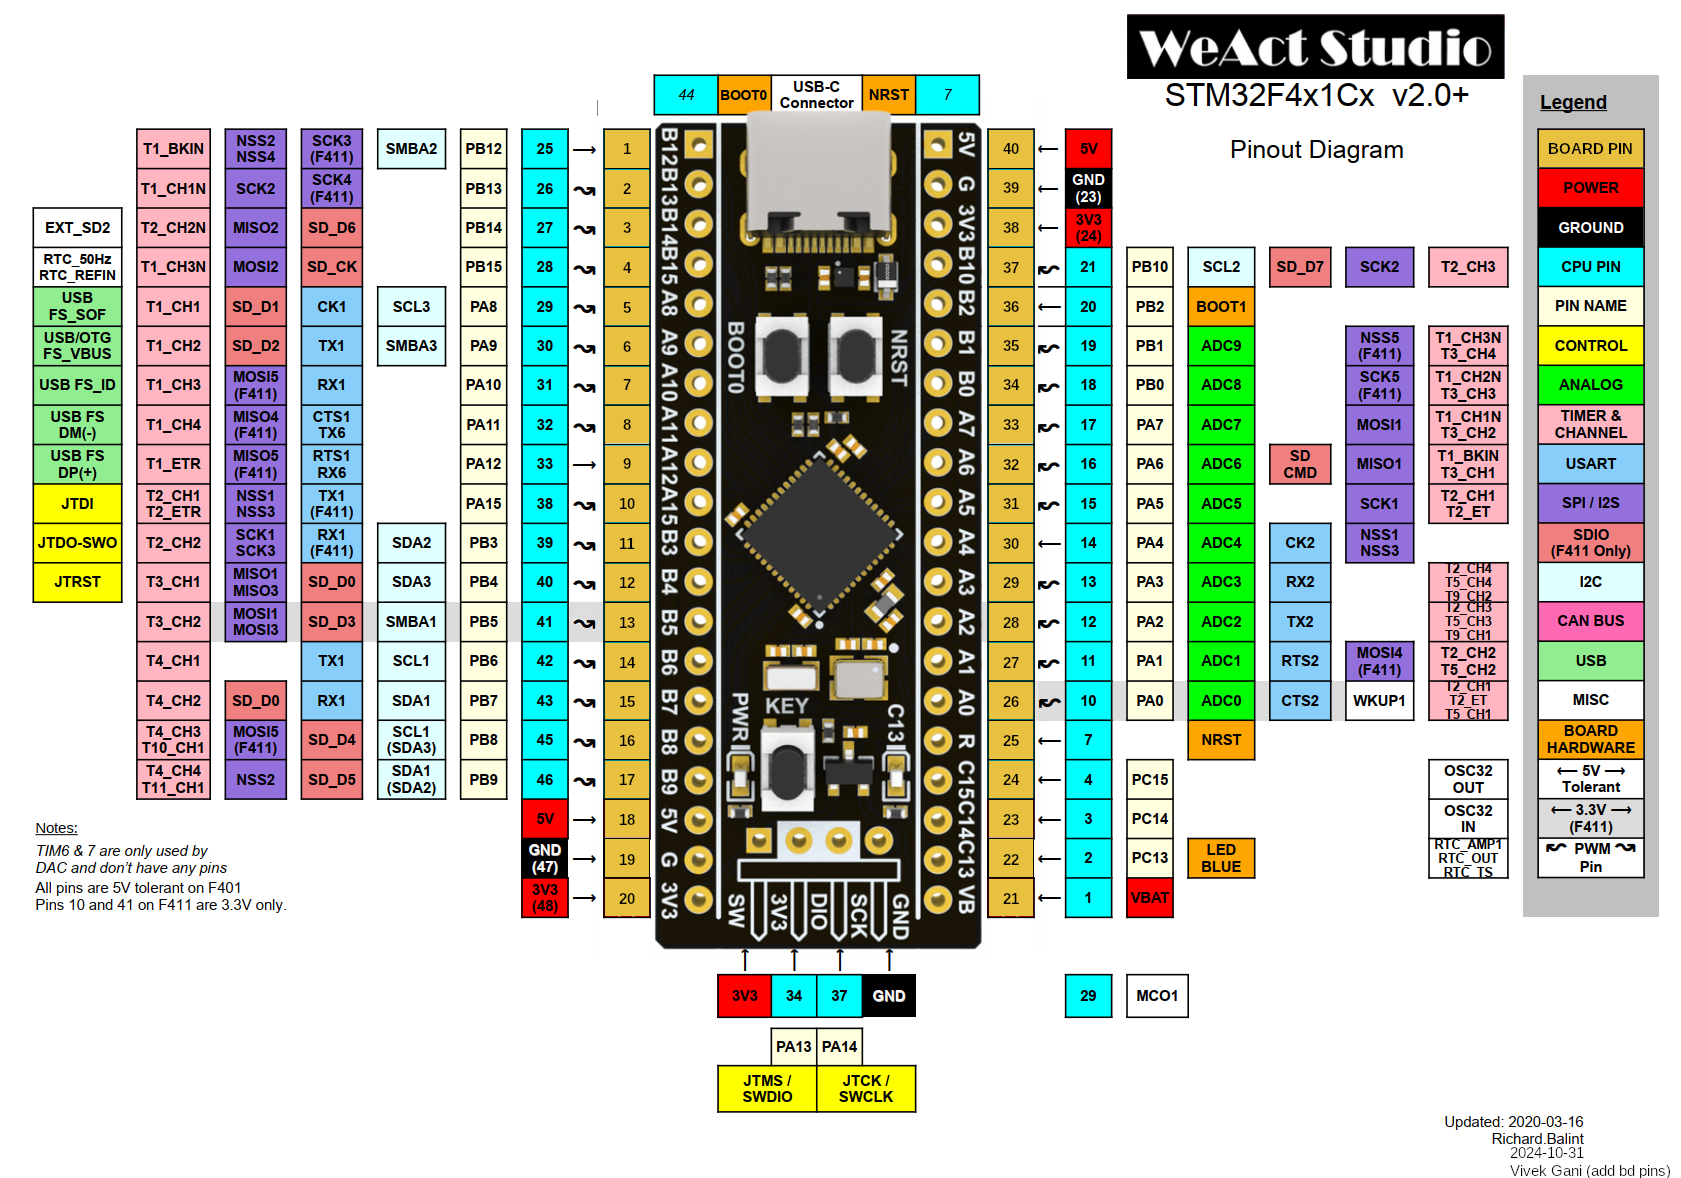
\includegraphics[width=0.8\textwidth]{images/hardware/STM32F4x1_PinoutDiagram_RichardBalint.png}
  \par\vspace{0.2cm}
  \footnotesize Fonte: WeActStudio, acesso em 22 abr. 2026.\footnote{Disponível em: \url{https://github.com/WeActStudio/WeActStudio.MiniSTM32F4x1}.}
\end{figure}

Com base na pinagem apresentada na Figura~\ref{fig:weact_github}, foram definidos os sinais utilizados pelo controlador de voo para comunicação com sensores, acionamento dos motores e troca de mensagens com o computador de missão. O Quadro~\ref{qua:pinos_stm32} resume os pinos reservados no protótipo e sua função na arquitetura embarcada.

\begin{quadro}[H]
  \centering
  \caption{Pinos da placa STM32F4x1 utilizados no protótipo.}
  \label{qua:pinos_stm32}
  \small
  \renewcommand{\arraystretch}{1.3}
  \begin{tabular}{|>{\centering\arraybackslash}p{2.4cm}|>{\raggedright\arraybackslash}p{10.5cm}|}
  \hline
  \textbf{Pinos usados} & \textbf{Função no protótipo} \\
  \hline
  PB10, PB3 & I$^2$C2 para IMU: SCL em PB10 e SDA em PB3. \\
  \hline
  PB4, PB5 & Interrupção e reset associados ao módulo BNO08X. \\
  \hline
  PB6--PB9 & Canais do TIM4 reservados para os quatro comandos DShot dos motores. \\
  \hline
  PA9, PA10 & USART1 para enlace UART com Raspberry Pi: TX em PA9 e RX em PA10. \\
  \hline
  PA2, PA3 & USART2 para o sensor MTF-01: TX em PA2 e RX em PA3. \\
  \hline
  PA4--PA7 & SPI1 para a memória \textit{flash} externa W25Q64: CS em PA4, SCK em PA5, MISO em PA6 e MOSI em PA7. \\
  \hline
  GND, 3V3, 5V & Referência comum e alimentação conforme os módulos conectados. \\
  \hline
  \end{tabular}
  \par\vspace{0.2cm}
  \footnotesize Fonte: elaborado pelos autores (2026).
\end{quadro}

% ----------------------------------------------------------------
\subsection{Sensores inerciais e de posição}\label{subsec:sensores}
% ----------------------------------------------------------------

A estimativa de estado do quadricóptero depende de dois sensores complementares:

\subsubsection{Unidade de Medição Inercial da família BNO08X}\label{subsubsec:bno08x}

O projeto adotou um módulo comercial BNO085, da família BNO08X. Essa família integra sensores inerciais e um hub de sensores capaz de disponibilizar \textit{reports} de aceleração, velocidade angular e vetores de rotação por meio da interface SH-2/SHTP \cite{bno08xdatasheet,sh2library}. A placa adquirida permite I$^2$C, e o projeto STM32 reserva I$^2$C2 a 400~kHz para essa interface.
Os vetores de rotação fornecidos pelo hub não dispensam a definição do estimador e dos sinais consumidos pelo controlador. O \textit{report} selecionado, taxa solicitada, taxa recebida, perda, \textit{jitter}, latência e comportamento sob vibração são medidos no conjunto real. Dessa maneira, limites de taxa publicados para uma saída específica não caracterizam garantia de que a malha completa opere nessa mesma frequência.

\subsubsection{Sensor de Fluxo Óptico e LiDAR MTF-01}\label{subsubsec:mtf01}

O MTF-01 é um módulo integrado que combina um sensor de fluxo óptico (PMW3901) e um LiDAR ToF (\textit{Time of Flight}) \cite{micoair2024}. O fluxo óptico mede movimento aparente da imagem; sua conversão em velocidade do veículo depende da distância ao solo, da orientação e da compensação da rotação. O LiDAR mede distância ao alvo no eixo de observação do sensor, que não coincide necessariamente com a altura vertical quando a aeronave está inclinada. O fabricante informa alcance de até 8~m sob condições especificadas, exatidão de 4~cm abaixo de 2~m a 90\% de refletância e 2\% acima de 2~m na mesma condição, além de alimentação de 5~V e interface UART a 115200~bit/s com protocolos Micolink, MAVLink e MSP \cite{micoairmtf01}. Assim, o MTF-01 fornece medições utilizadas na estimação e no controle de posição e altura, sem fornecer posição absoluta por si só.

\begin{figure}[H]
    \centering
    \caption{Pinagem do MTF-01.}
    \label{fig:mtf01}
    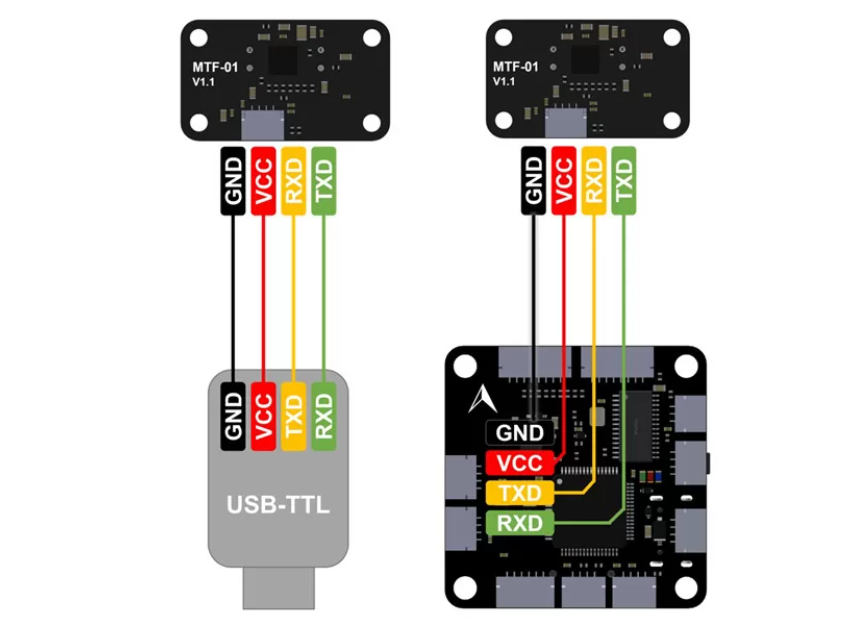
\includegraphics[width=0.5\textwidth]{images/hardware/MTF01Scheme.png}
    \fonte{MicoAir, acesso em 09 set. 2026.\footnote{Disponível em: \url{https://micoair.com/optical_range_sensor_mtf-01/}.}}
\end{figure}

O controlador atua sobre o estado estimado $\hat{\mathbf{x}}$, não sobre o estado verdadeiro diretamente. A arquitetura do protótipo deve registrar quais \textit{reports} do BNO08X são usados para atitude e velocidades angulares, como os eixos dos sensores são transformados para o referencial do corpo, como fluxo óptico e distância são convertidos em velocidade e posição relativa, como sinais com taxas diferentes são sincronizados, como a origem local é inicializada e como a deriva é tratada. Caso seja introduzido um estimador adicional no STM32, ele deve ser documentado como componente próprio, com parâmetros, taxas e método de validação.

% Protocolo MAVLink e comunicação confiável entre Raspberry Pi e STM32
% ============================================================================
% REFERENCIAL TEÓRICO — protocolo MAVLink e comunicação confiável entre o
% computador de missão e o controlador de voo.
% Chamado em partes/textuais/referencial_teorico.tex, na seção de sistemas
% embarcados e comunicação.
% ============================================================================

% ----------------------------------------------------------------
\subsection{Protocolo MAVLink}\label{subsec:mavlink}
% ----------------------------------------------------------------

O MAVLink (\textit{Micro Air Vehicle Link}) é um protocolo de mensagens binárias leve, projetado para sistemas com recursos limitados e enlaces de comunicação com largura de banda restrita \cite{koubaa2019, mavlinkguide}. É o protocolo utilizado pelos pilotos automáticos de código aberto PX4 e ArduPilot e por estações de solo como o QGroundControl, o que o tornou um padrão de fato na comunicação com VANTs \cite{koubaa2019}. Ele suporta fluxos periódicos de telemetria e microsserviços como missões, parâmetros e comandos; confirmações, retransmissões e semântica de conclusão dependem do microsserviço e da implementação adotada \cite{mavlinkguide}.

As mensagens são definidas em arquivos XML, que descrevem, para cada mensagem, seu identificador numérico, seus campos, os tipos e as unidades. O arquivo \texttt{common.xml} provê a maioria das mensagens utilizadas por pilotos automáticos e estações de controle, e um projeto pode criar um \textbf{dialeto} próprio, isto é, um XML que inclui o \texttt{common.xml} e acrescenta mensagens e enumerações específicas \cite{mavlinkguide}. A partir do XML, o gerador oficial (\texttt{mavgen}) produz o código de empacotamento e desempacotamento para diferentes linguagens; para sistemas embarcados como o STM32F411, a implementação de referência é uma biblioteca C \textit{header-only}, otimizada para o uso eficiente de RAM e \textit{Flash}, e, para Python, a biblioteca \texttt{pymavlink} \cite{koubaa2019, mavlinkguide}. Como os dois lados do enlace são gerados da mesma definição, a estrutura das mensagens é necessariamente a mesma em ambos.

No MAVLink 2, cada mensagem é transmitida em um pacote com a estrutura do Quadro~\ref{qua:mavlink_pacote}. O byte inicial permite ao receptor ressincronizar-se após a perda ou corrupção de bytes, procurando o próximo início de pacote; o número de sequência permite detectar pacotes perdidos; e os identificadores de sistema e componente indicam o remetente. Zeros no fim do \textit{payload} são omitidos na transmissão e restaurados na recepção, o que reduz o tamanho das mensagens \cite{mavlinkguide}.

\begin{quadro}[H]
    \centering
    \caption{Estrutura do pacote MAVLink 2.}
    \label{qua:mavlink_pacote}
    \small
    \renewcommand{\arraystretch}{1.3}
    \begin{tabular}{|>{\raggedright\arraybackslash}p{3.4cm}|>{\centering\arraybackslash}p{1.6cm}|>{\raggedright\arraybackslash}p{8.4cm}|}
        \hline
        \textbf{Campo} & \textbf{Bytes} & \textbf{Função} \\
        \hline
        Início (\texttt{0xFD}) & 1 & Marca o começo do pacote e permite a ressincronização. \\
        \hline
        Comprimento & 1 & Tamanho do \textit{payload}, de 0 a 255 \textit{bytes}. \\
        \hline
        \textit{Flags} & 2 & Indicações de compatibilidade, como o uso de assinatura. \\
        \hline
        Sequência & 1 & Contador de pacotes do remetente; saltos indicam perdas. \\
        \hline
        \textit{System ID} & 1 & Veículo ou sistema que enviou a mensagem. \\
        \hline
        \textit{Component ID} & 1 & Componente do sistema que enviou a mensagem. \\
        \hline
        \textit{Message ID} & 3 & Identificador da mensagem (até 16\,777\,215). \\
        \hline
        \textit{Payload} & 0 a 255 & Campos da mensagem em binário. \\
        \hline
        \textit{Checksum} & 2 & CRC-16/MCRF4XX do pacote, incluindo o \texttt{CRC\_EXTRA}. \\
        \hline
        Assinatura (opcional) & 13 & Autenticação da origem. \\
        \hline
    \end{tabular}
    \par\vspace{0.2cm}
    \footnotesize Fonte: elaborado pelos autores (2026), com base em \citeonline{mavlinkguide}.
\end{quadro}

No padrão MAVLink v1, o protocolo acrescenta 8~\textit{bytes} ao \textit{payload}. No MAVLink v2 sem assinatura, são acrescentados 12~\textit{bytes}; quando a assinatura opcional é usada, acrescentam-se mais 13~\textit{bytes}, totalizando 25~\textit{bytes} além do \textit{payload} \cite{mavlinkguide,mavlinksigning}. A integridade contra corrupção acidental é verificada por um \textit{checksum} CRC-16/MCRF4XX. O \texttt{CRC\_EXTRA}, um valor calculado a partir da definição da mensagem no XML, participa do cálculo desse \textit{checksum}: se emissor e receptor usarem definições diferentes para a mesma mensagem, o \textit{checksum} não confere e a mensagem é descartada, em vez de ser interpretada de forma errada. Ele não é um segundo \textit{checksum} transmitido separadamente \cite{mavlinkguide}.

Entre os microsserviços padronizados, destacam-se o \textit{HEARTBEAT}, mensagem periódica pela qual cada componente anuncia sua presença, seu tipo e seu estado, e cuja ausência indica a perda do enlace; o protocolo de comandos (\texttt{COMMAND\_LONG} e \texttt{COMMAND\_ACK}), em que cada comando recebe uma resposta com o resultado; e o protocolo de parâmetros (\texttt{PARAM\_*}), que permite ler e alterar valores de configuração do veículo durante a operação \cite{mavlinkguide}.

% ----------------------------------------------------------------
\subsection{Comunicação confiável entre o computador de missão e o controlador de voo}\label{subsec:comunicacao_confiavel}
% ----------------------------------------------------------------

Um enlace serial pode perder, corromper ou atrasar mensagens. O \textit{checksum} descarta mensagens corrompidas, mas não garante que uma mensagem chegue. Para que um comando seja executado com segurança, o protocolo de aplicação precisa de confirmações e de retransmissão: o emissor reenvia o pedido quando não recebe resposta dentro de um prazo. A retransmissão, porém, cria um problema: se o pedido foi executado e apenas a resposta se perdeu, o reenvio pode fazer o receptor executá-lo duas vezes \cite{tanenbaum2007}.

Para comandos que movem um veículo, a execução duplicada é inaceitável: um deslocamento de 1~m executado duas vezes leva o veículo a 2~m. A solução usual é tornar o pedido \textbf{idempotente}: cada pedido recebe um identificador único, o receptor guarda os pedidos já tratados e, ao receber um pedido repetido, apenas reenvia a resposta já dada, sem executá-lo de novo. Essa garantia é conhecida como semântica de \textbf{no máximo uma vez} (\textit{at-most-once}) \cite{tanenbaum2007}.

Também é necessário que o controlador de voo detecte a falha do computador de missão. Mensagens periódicas, como o \textit{HEARTBEAT}, funcionam como um \textit{watchdog} do enlace: se deixam de chegar por um tempo definido, o controlador assume que a comunicação foi perdida e executa uma ação segura, como manter a posição ou pousar \cite{mavlinkguide}. O mesmo princípio pode ser aplicado a uma autorização explícita do operador, renovada periodicamente, de forma análoga ao dispositivo de homem morto (\textit{dead man's switch}): o veículo só executa novos movimentos enquanto essa autorização continua a ser recebida.


% ----------------------------------------------------------------
\subsection{Protocolo DShot}\label{subsec:dshot}
% ----------------------------------------------------------------

O DShot (\textit{Digital Shot}) é um protocolo digital de comunicação entre o controlador de voo e os Controladores Eletrônicos de Velocidade (ESCs --- do inglês \textit{Electronic Speed Controllers}). Diferentemente dos protocolos analógicos tradicionais baseados em PWM (\textit{Pulse Width Modulation}), a trama possui 16~\textit{bits}: 11~\textit{bits} de valor, 1~\textit{bit} de solicitação de telemetria e 4~\textit{bits} de CRC. Os valores 0 e 1--47 são reservados; os comandos de \textit{throttle} ocupam a faixa 48--2047, totalizando 2000 níveis \cite{betaflightdshot}.

As principais vantagens do DShot sobre protocolos analógicos são \cite{idrissi2022}:

\begin{alineastcc}
    \item \textbf{verificação de integridade}: a codificação digital e o CRC ajudam a detectar erros de transmissão, embora o sinal continue sujeito a ruído, problemas de temporização e falhas elétricas;
    \item \textbf{resolução}: 2000 níveis de \textit{throttle} úteis, além dos valores reservados do protocolo;
    \item \textbf{ausência de calibração dos extremos de \textit{throttle}}: não é necessário definir pulsos mínimo e máximo como em protocolos PWM, embora a configuração do ESC e a caracterização de empuxo permaneçam necessárias;
    \item \textbf{temporização definida}: variantes como DShot600 usam taxa de linha de 600~kbit/s; a frequência prática de atualização depende da versão, da telemetria e da implementação \cite{betaflightdshot}.
\end{alineastcc}

No STM32F411, a implementação utiliza temporizador e DMA (\textit{Direct Memory Access}) para reduzir a intervenção do processador na transmissão. A compatibilidade entre o período da malha e a geração do sinal depende da medição elétrica do DShot e da integração com o ESC.

\clearpage
\chapter{MATERIAIS E MÉTODOS}\label{cap:metodologia}

Este capítulo descreve os materiais, a arquitetura, os procedimentos de desenvolvimento e os critérios de avaliação da plataforma experimental. Após a obtenção do modelo completo, é necessário obter a estabilização do sistema. Toda a estruturação e aplicação de técnicas de controle é realizada e validada no \textit{software} MATLAB/Simulink e posteriormente implementada no \textit{firmware} do controlador de voo. A validação do desempenho do sistema ocorre em ambiente interno, com o objetivo de reduzir riscos e permitir a coleta de dados confiáveis.

O objeto de estudo é um quadricóptero em configuração X destinado à validação de estabilização, telemetria e execução de missões simplificadas em ambiente interno. A arquitetura distribui responsabilidades entre um controlador de voo baseado em STM32F411 e um computador de missão Raspberry Pi Zero W. O STM32 executa as funções críticas de aquisição de sensores, estimação, controle, mistura de motores, geração de comandos DShot e \textit{failsafes}. O Raspberry Pi executa serviços de missão, comunicação em rede, roteamento e registro de telemetria; portanto, sua indisponibilidade não deve impedir o controlador de voo de entrar em estado seguro.

A comunicação entre as camadas é especificada como DroneLink (Seção~\ref{subsec:metodo_comunicacao}), uma camada própria do projeto executada sobre UART com enquadramento MAVLink 2. MAVLink é um protocolo de mensagens binárias desenvolvido para sistemas com recursos limitados e prevê identificação de sistemas/componentes, telemetria e mecanismos de integridade de mensagens \cite{koubaa2019,mavlinkguide}. No DroneLink, a rota calculada pelo módulo de planejamento é convertida em trechos de missão (\textit{legs}, na nomenclatura do protocolo: o deslocamento entre dois pontos consecutivos da rota) com identificação, confirmação, timeout e tratamento de duplicidade; o protocolo não substitui as proteções locais do controlador de voo, e o Raspberry Pi nunca envia PWM, DShot ou comandos diretos de motor.

\section{MATERIAIS E AMBIENTE DE EXECUÇÃO}\label{sec:materiais_ambiente}

Os componentes físicos da plataforma foram separados por função para facilitar a montagem, a inspeção visual e a rastreabilidade dos ensaios. A Figura~\ref{fig:componentes_principais} ilustra os principais módulos utilizados: controlador STM32F411, Raspberry Pi Zero W, unidade inercial BNO08X, sensor MicoAir MTF-01, ESC, motores, hélices, estrutura e elementos de alimentação. As imagens servem para identificar fisicamente os itens descritos no Quadro~\ref{qua:componentes}; especificações elétricas, versões e parâmetros de uso permanecem registrados no texto e nos quadros.

\newcommand{\componente}[2]{%
    \begin{minipage}[t]{0.30\textwidth}
        \centering
        \parbox[c][3.0cm][c]{\linewidth}{%
            \centering
            \includegraphics[
                width=\linewidth,
                height=2.9cm,
                keepaspectratio
            ]{#1}%
        }
        \par\vspace{0.08cm}
        {\footnotesize #2\par}
    \end{minipage}%
}

\begin{figure}[H]
    \centering
    \caption{Principais componentes físicos da plataforma experimental.}
    \label{fig:componentes_principais}

    \noindent
    \componente
        {images/hardware/STM32.png}
        {Controlador STM32F411}
    \hfill
    \componente
        {images/hardware/RPIZEROW16GB.png}
        {Raspberry Pi Zero W com SD de 16 GB}
    \hfill
    \componente
        {images/hardware/GY-BNO08X.png}
        {IMU BNO08X}

    \par\vspace{0.35cm}

    \noindent
    \componente
        {images/hardware/MTF01.png}
        {MicoAir MTF-01}
    \hfill
    \componente
        {images/hardware/ESC.jpg}
        {ESC 4 em 1}
    \hfill
    \componente
        {images/hardware/MOTOR-HELICE.png}
        {Motor e hélice}

    \par\vspace{0.35cm}

    \noindent
    \componente
        {images/hardware/GERPC.png}
        {Estrutura}
    \hfill
    \componente
        {images/hardware/BEC.png}
        {BEC}
    \hfill
    \componente
        {images/hardware/FONTECHAVEADA.png}
        {Fonte chaveada}

    \par\vspace{0.35cm}

    \noindent
    \hfill
    \componente
        {images/hardware/bateria_leao.png}
        {Bateria LiPo 3S}
    \hfill
    \componente
        {images/hardware/b6neo.png}
        {Carregador balanceador}
    \hfill\null

    \par\vspace{0.25cm}
    \begin{minipage}{0.95\textwidth}
        \centering
        \footnotesize Fonte: montagem elaborada pelos autores (2026); fotografias do Raspberry Pi Zero W e do conjunto motor--hélice dos autores; demais imagens obtidas por busca no Google Imagens.
    \end{minipage}
\end{figure}

O Quadro~\ref{qua:componentes} registra os principais materiais e especificações da plataforma experimental. Especificações comerciais são identificadas como tal; dados que dependem do exemplar físico, como a versão gravada do ESC, não são inferidos a partir de anúncios.

\begin{quadro}[htb]
\centering
\caption{Componentes da plataforma experimental.}
\label{qua:componentes}
\small
\renewcommand{\arraystretch}{1.3}
\begin{tabular}{
  |
  >{\raggedright\arraybackslash}p{3.2cm}
  |
  >{\raggedright\arraybackslash}p{10.8cm}
  |
}
\hline
\textbf{Função} & \textbf{Componente ou especificação} \\
\hline

Controlador de voo &
WeAct Studio MiniSTM32F4x1/Black Pill V3.1\newline
STM32F411CEU6, variante com HSE de 25~MHz\newline
Cortex-M4F, até 100~MHz, 512~kB de Flash e 128~kB de SRAM \cite{stm32f411ds}. \\[4pt]
\hline

Computador de missão &
Raspberry Pi Zero W v1.1\newline
BCM2835/ARMv6, 512~MB. \\[4pt]
\hline

IMU &
Módulo da família BNO08X; identificação específica a registrar por marcação física ou leitura do Product ID. \\[4pt]
\hline

Fluxo e altura &
MicoAir MTF-01; fluxo óptico, LiDAR ToF, UART 115200~bit/s e alimentação de 5~V segundo especificação do fabricante \cite{micoairmtf01}. \\[4pt]
\hline

Controlador de velocidade (ESC) &
Skystars KM55A II 4 em 1 (AM32 Turbo, 2024), AT32F421, 3S--6S, DShot300/DShot600/PWM. \\[4pt]
\hline

Propulsores (motores e hélices) &
4x Motores GEPRC SPEEDX2 2105.5, 2650KV. \newline
4x Hélices Gemfan D90-3. \\[4pt]
\hline

Estrutura &
Frame GEPRC CineLog35 V3, 3,5 polegadas. \\[4pt]
\hline

Energia &
1x Bateria Leão LB2200LP3, LiPo 3S (11,1~V), 2200~mAh, 30C.\newline
1x Micro BEC EXUAVRC/VTX BEC 2S--6S.\newline
1x capacitor de 680~$\mu$F, 35~V, baixo ESR. \\[4pt]
\hline

Carregador de bateria &
SkyRC B6neo 2, carregador balanceador para baterias LiPo. \\[4pt]
\hline

Fonte de bancada (Testes) &
Lumiville chaveada estabilizada bivolt, 12~V/50~A, 600~W; saída regulável de 12~V a 14~V. \\
\hline
\end{tabular}
\par\vspace{0.2cm}
\footnotesize Fonte: elaborado pelos autores (2026).
\end{quadro}

O módulo BNO08X implementa um hub de sensores com interface SH-2/SHTP. A biblioteca pública SH-2 disponibiliza, entre outros, \textit{reports} de acelerômetro, giroscópio, vetores de rotação e o acesso à identificação do produto \cite{sh2library}. A escolha do tipo de \textit{report}, sua taxa configurada e a latência efetivamente observada são registradas no ensaio, pois um limite publicado para uma saída específica não garante a mesma taxa para todas as saídas nem para a malha completa de controle \cite{bno08xdatasheet}.

A Figura~\ref{fig:prototipo_montado} apresenta a montagem final do protótipo em seis vistas, permitindo observar a distribuição dos módulos eletrônicos, da bateria, dos motores e das conexões sobre a estrutura. As indicações de direita e esquerda correspondem aos lados do próprio drone, considerando sua direção frontal, e não aos lados de quem observa a fotografia. A vista inferior evidencia a instalação do sensor de fluxo óptico e distância voltado para o solo.

\begin{figure}[htbp]
    \centering
    \caption{Montagem final do protótipo em seis vistas.}
    \label{fig:prototipo_montado}
    \begin{minipage}[t]{0.31\textwidth}
        \centering
        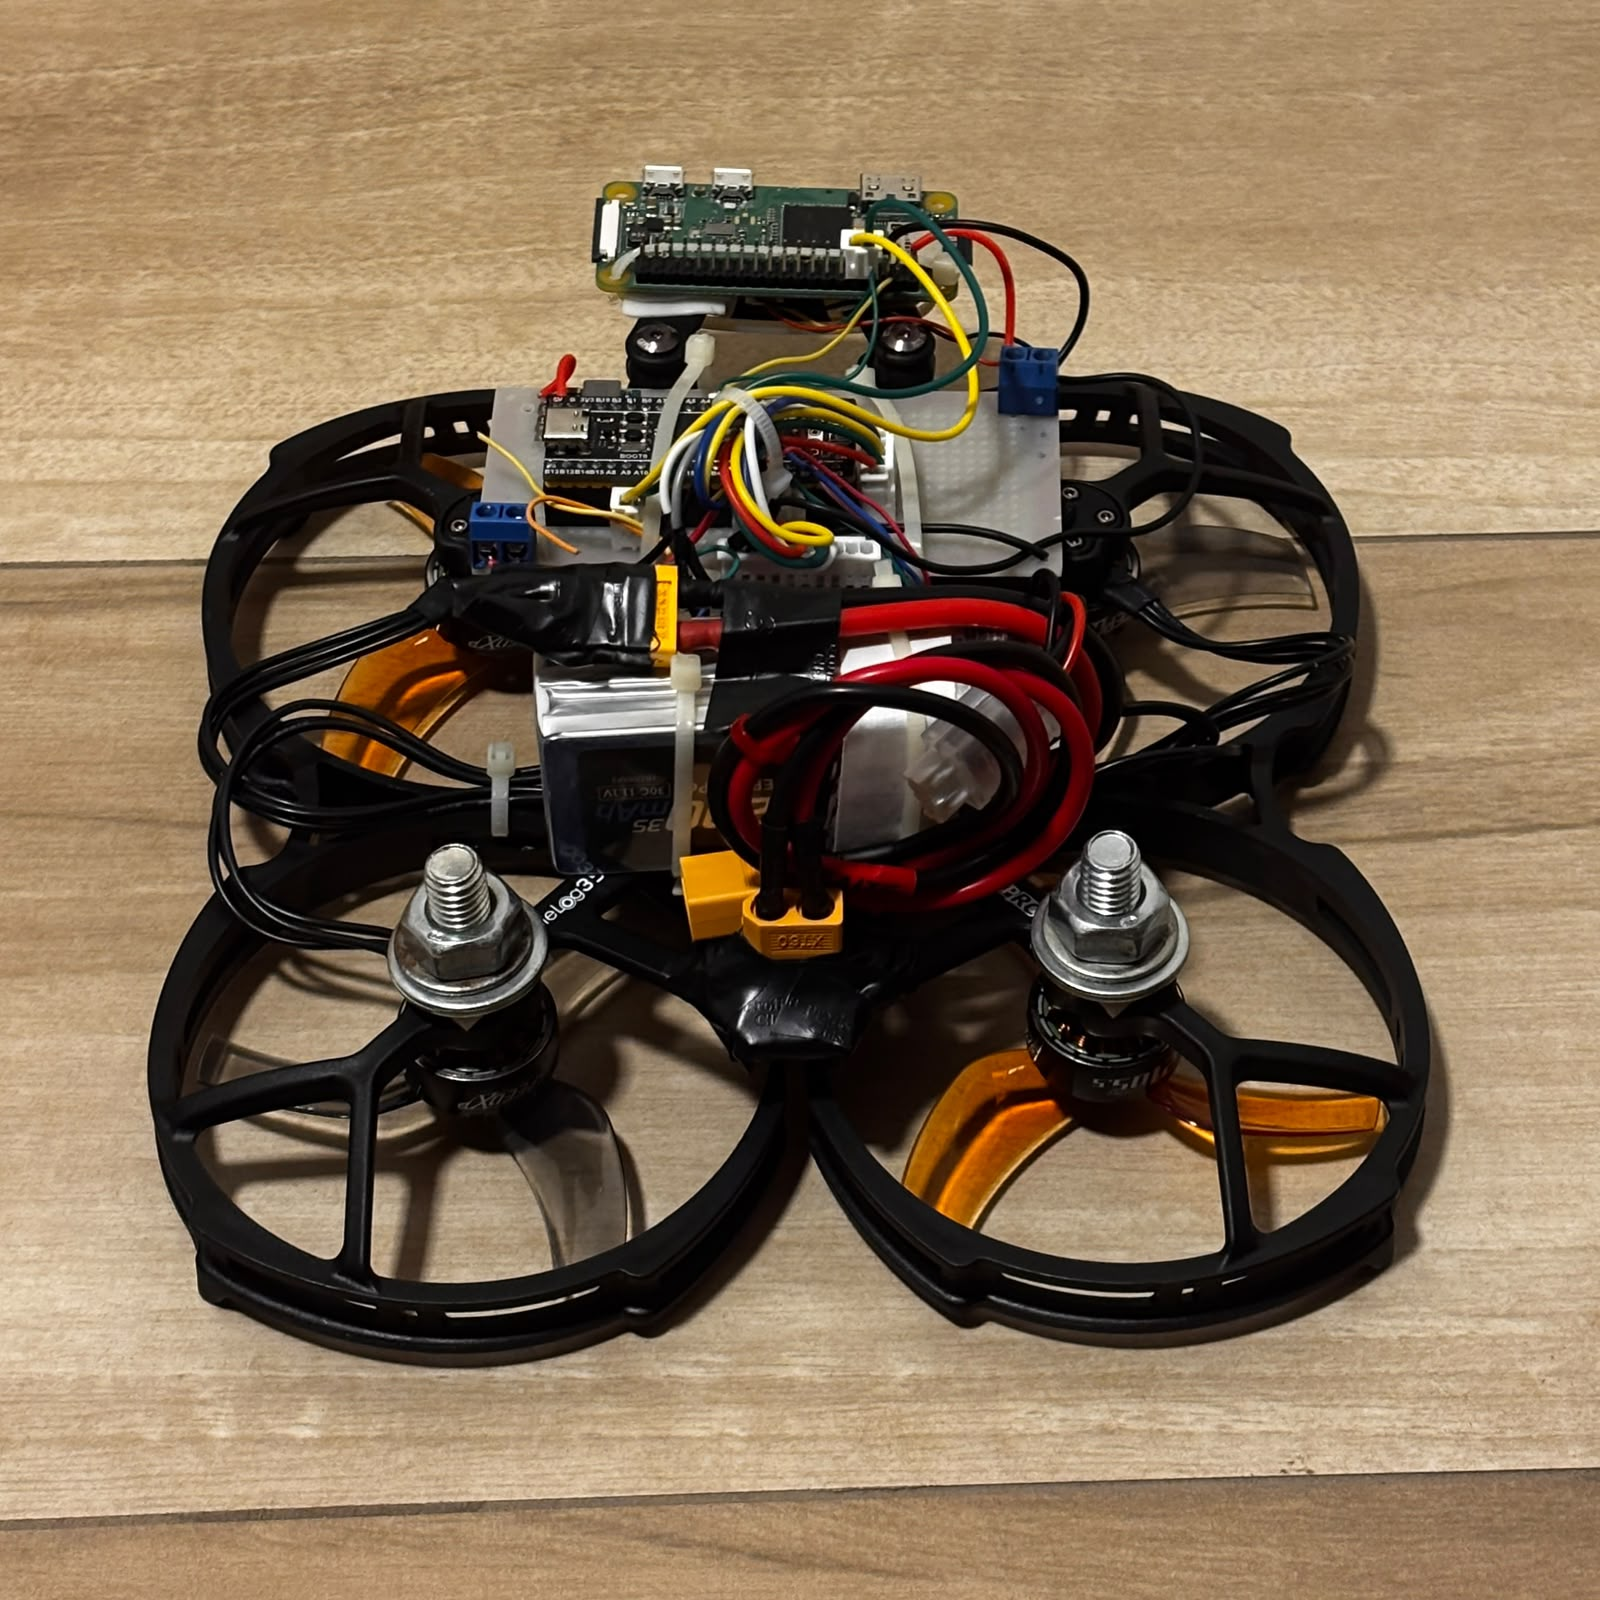
\includegraphics[width=\linewidth,height=4.4cm,keepaspectratio]{images/hardware/prototipo/drone_frente.jpeg}
        \par\smallskip{\footnotesize (a) Vista frontal}
    \end{minipage}
    \hfill
    \begin{minipage}[t]{0.31\textwidth}
        \centering
        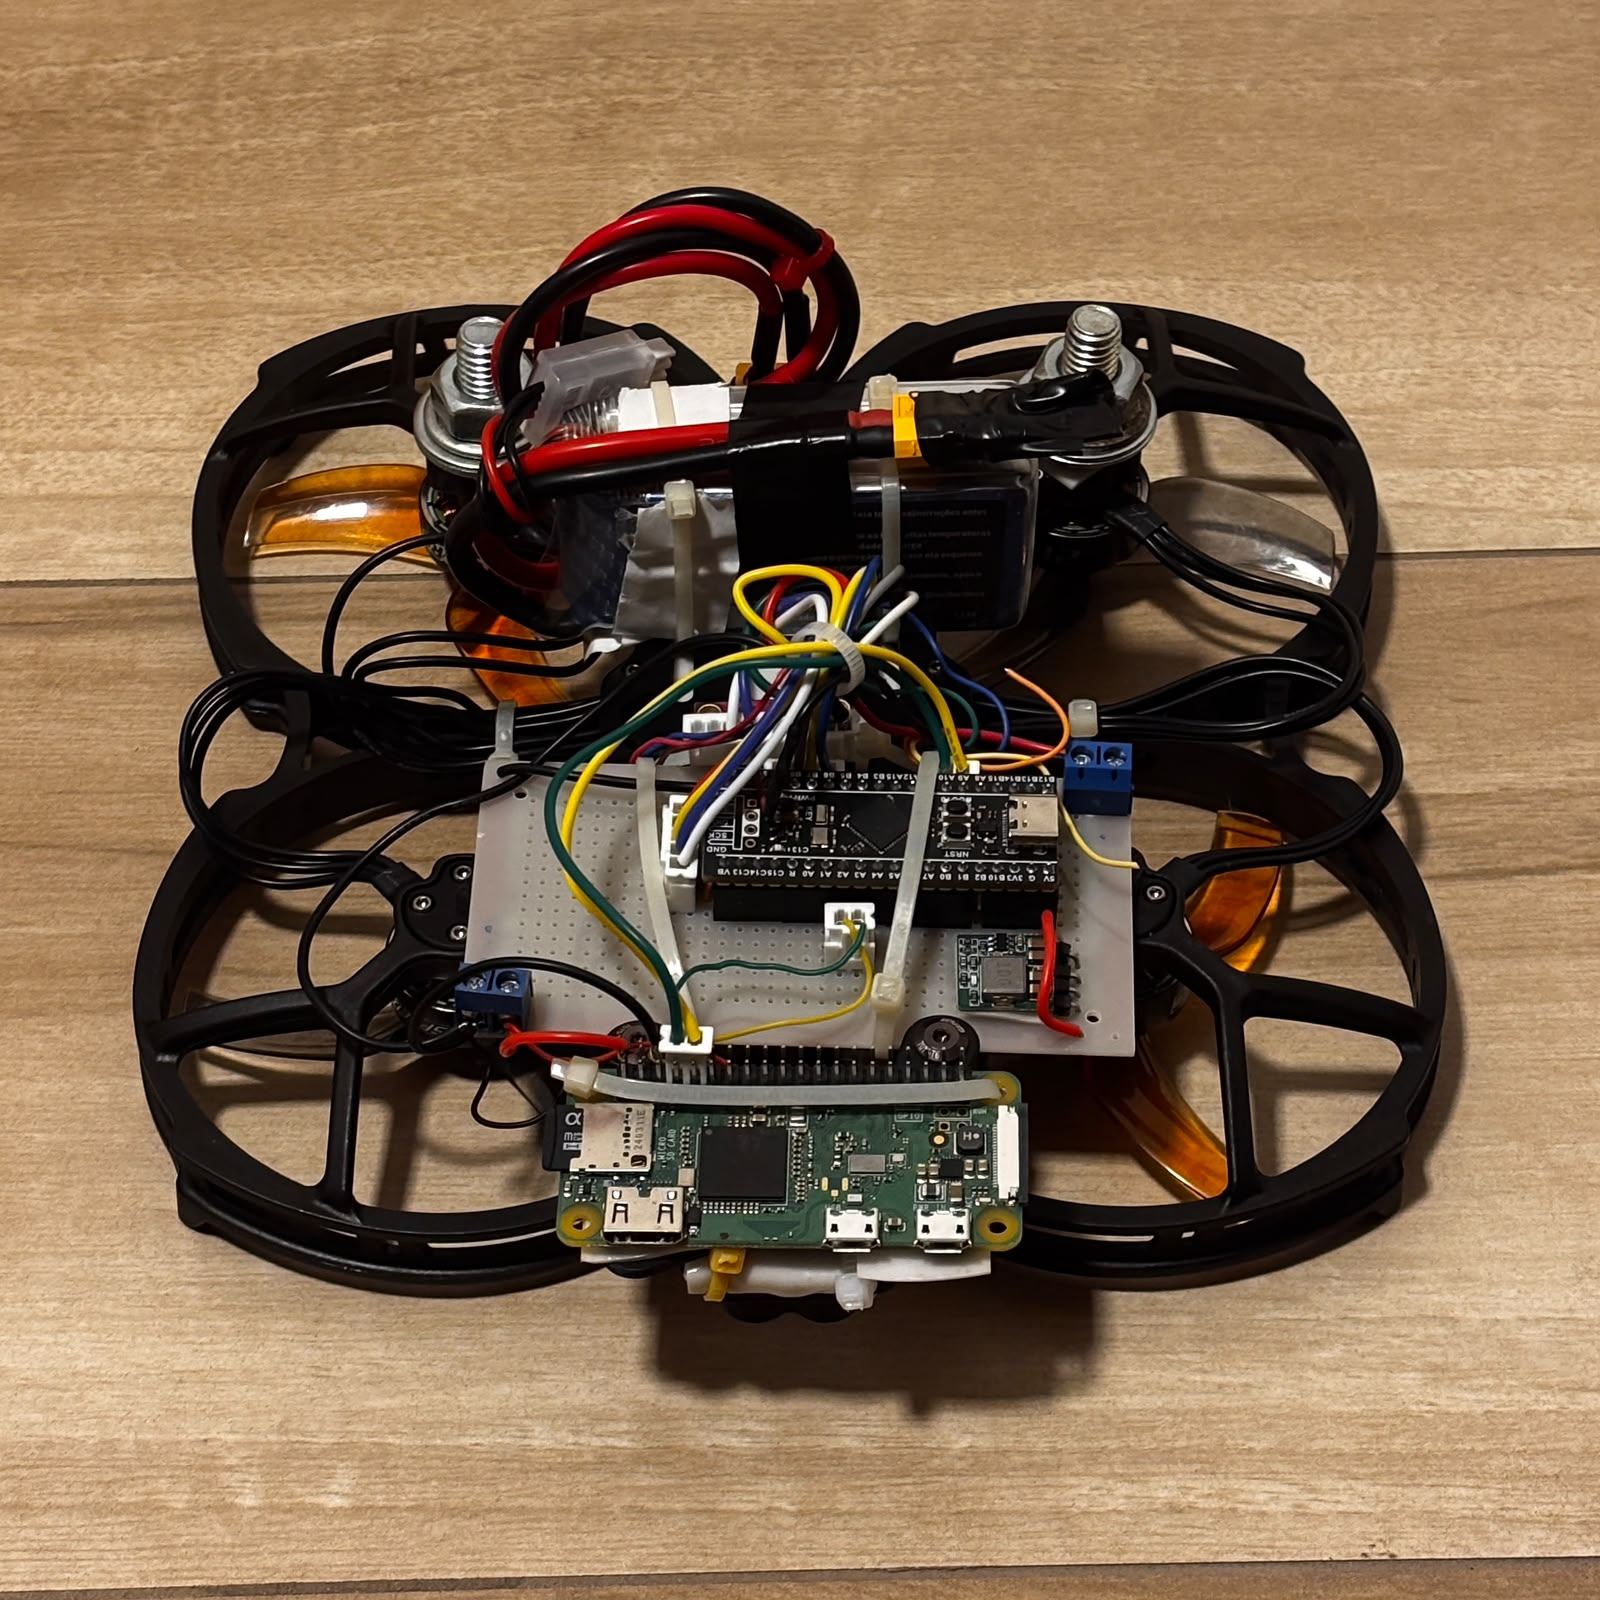
\includegraphics[width=\linewidth,height=4.4cm,keepaspectratio]{images/hardware/prototipo/drone_traseira.jpeg}
        \par\smallskip{\footnotesize (b) Vista traseira}
    \end{minipage}
    \hfill
    \begin{minipage}[t]{0.31\textwidth}
        \centering
        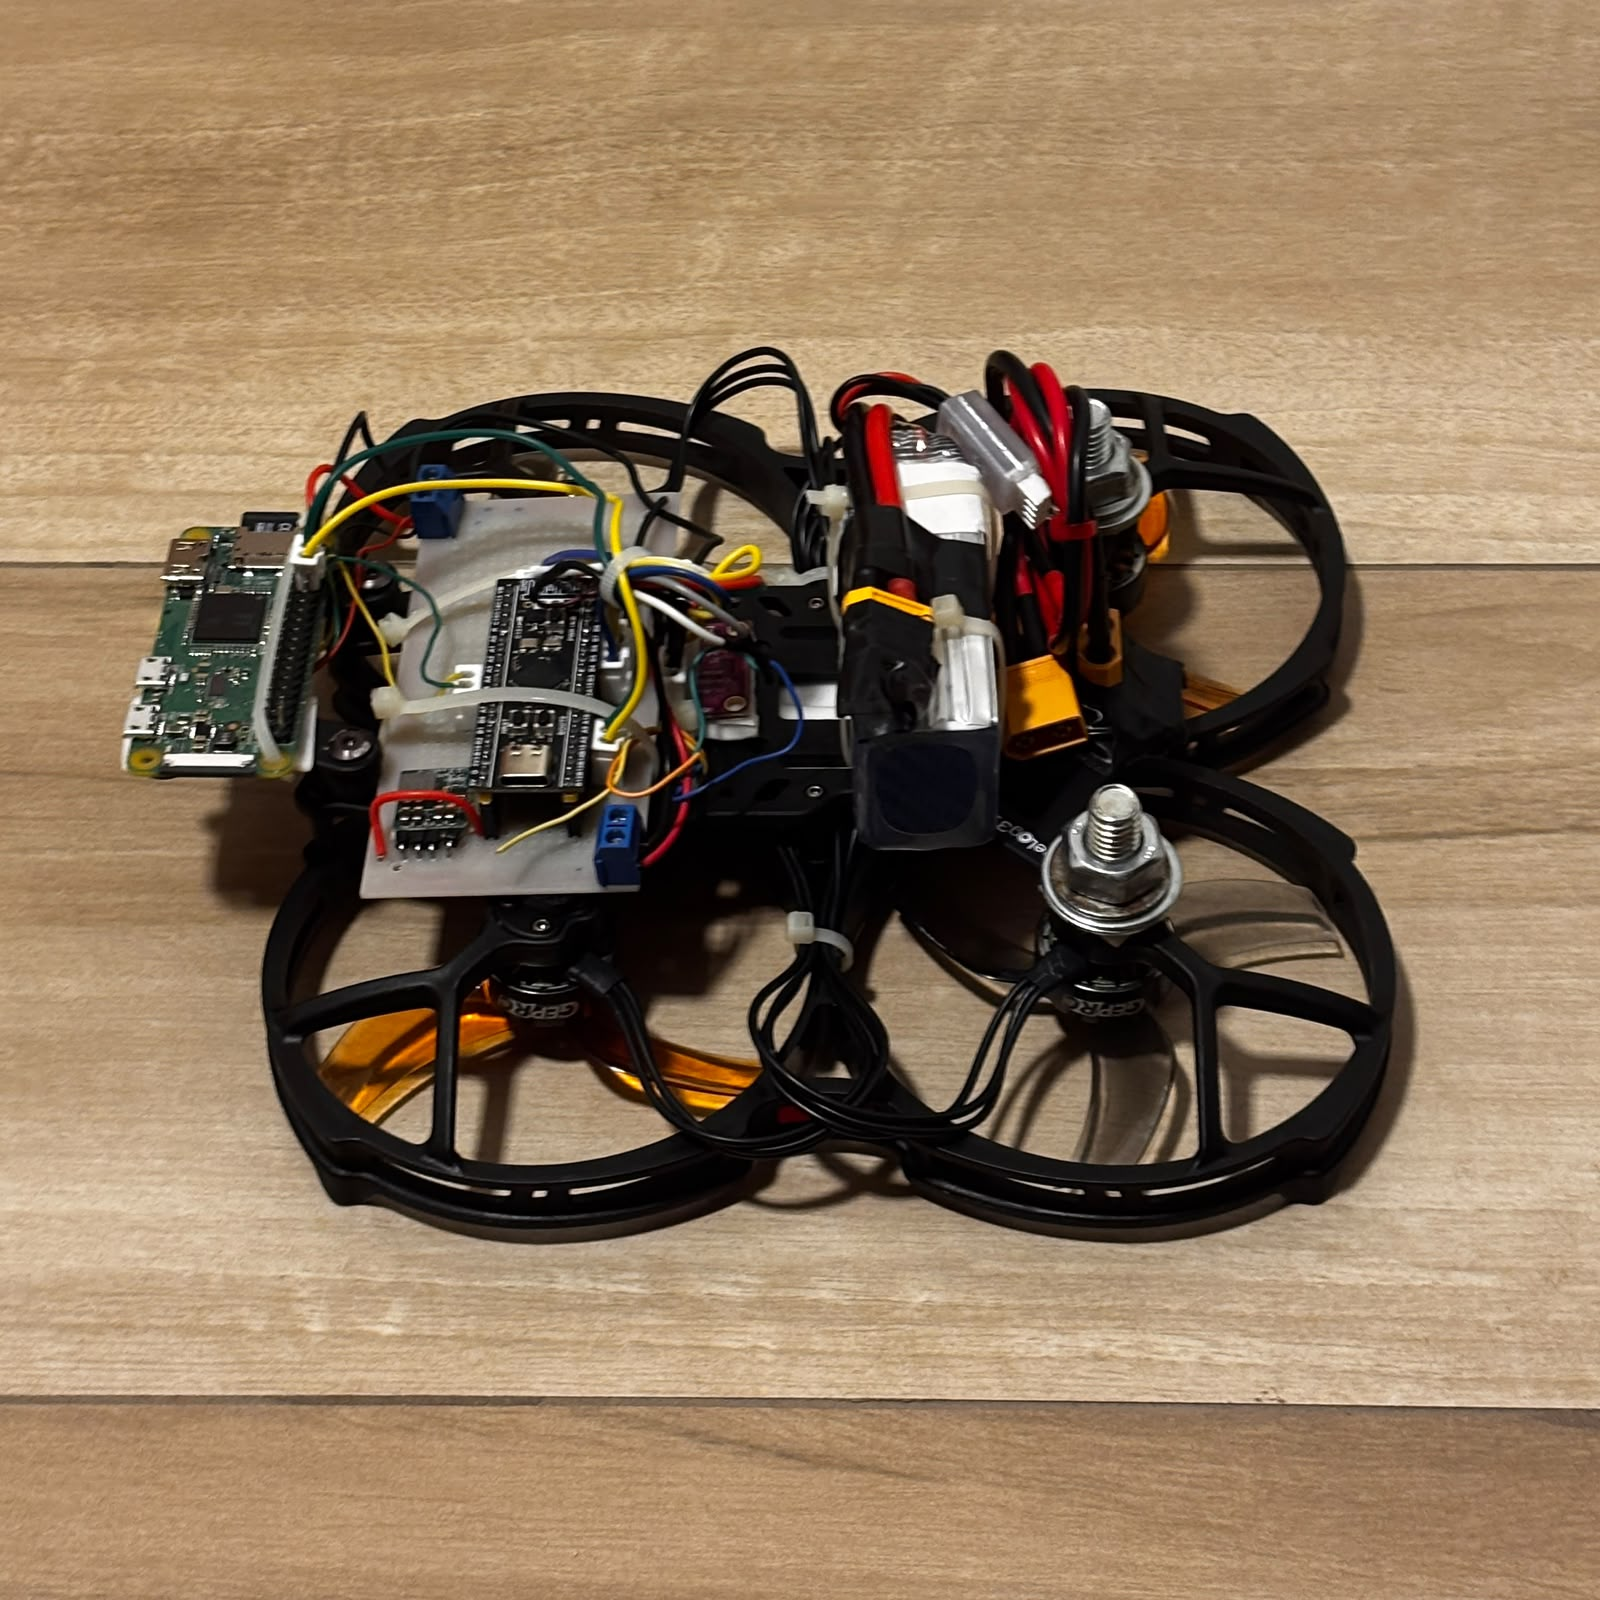
\includegraphics[width=\linewidth,height=4.4cm,keepaspectratio]{images/hardware/prototipo/drone_direita.jpeg}
        \par\smallskip{\footnotesize (c) Lateral direita}
    \end{minipage}
    \par\vspace{0.25cm}
    \begin{minipage}[t]{0.31\textwidth}
        \centering
        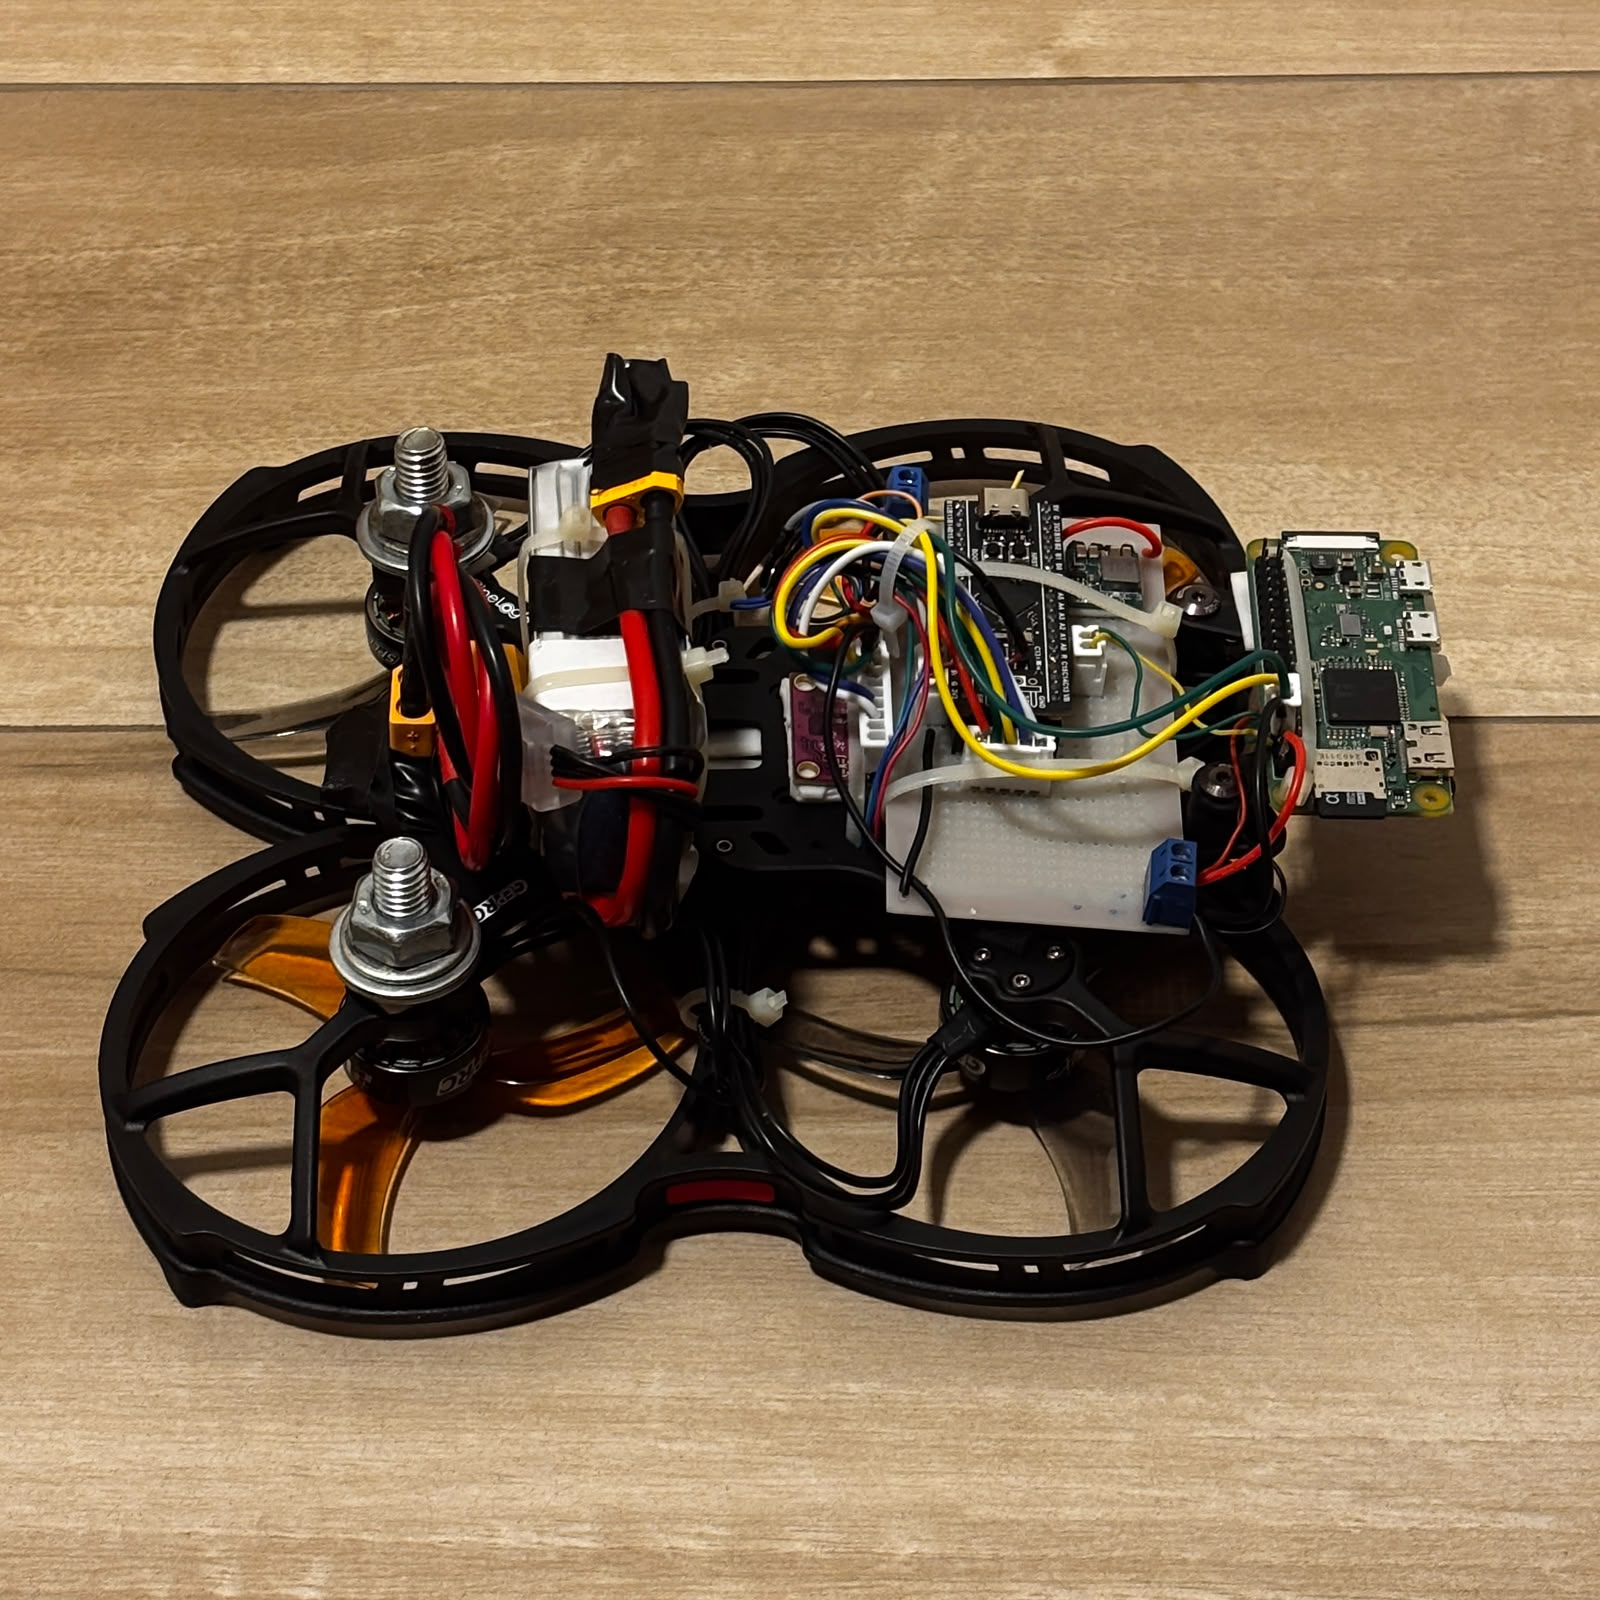
\includegraphics[width=\linewidth,height=4.4cm,keepaspectratio]{images/hardware/prototipo/drone_esquerda.jpeg}
        \par\smallskip{\footnotesize (d) Lateral esquerda}
    \end{minipage}
    \hfill
    \begin{minipage}[t]{0.31\textwidth}
        \centering
        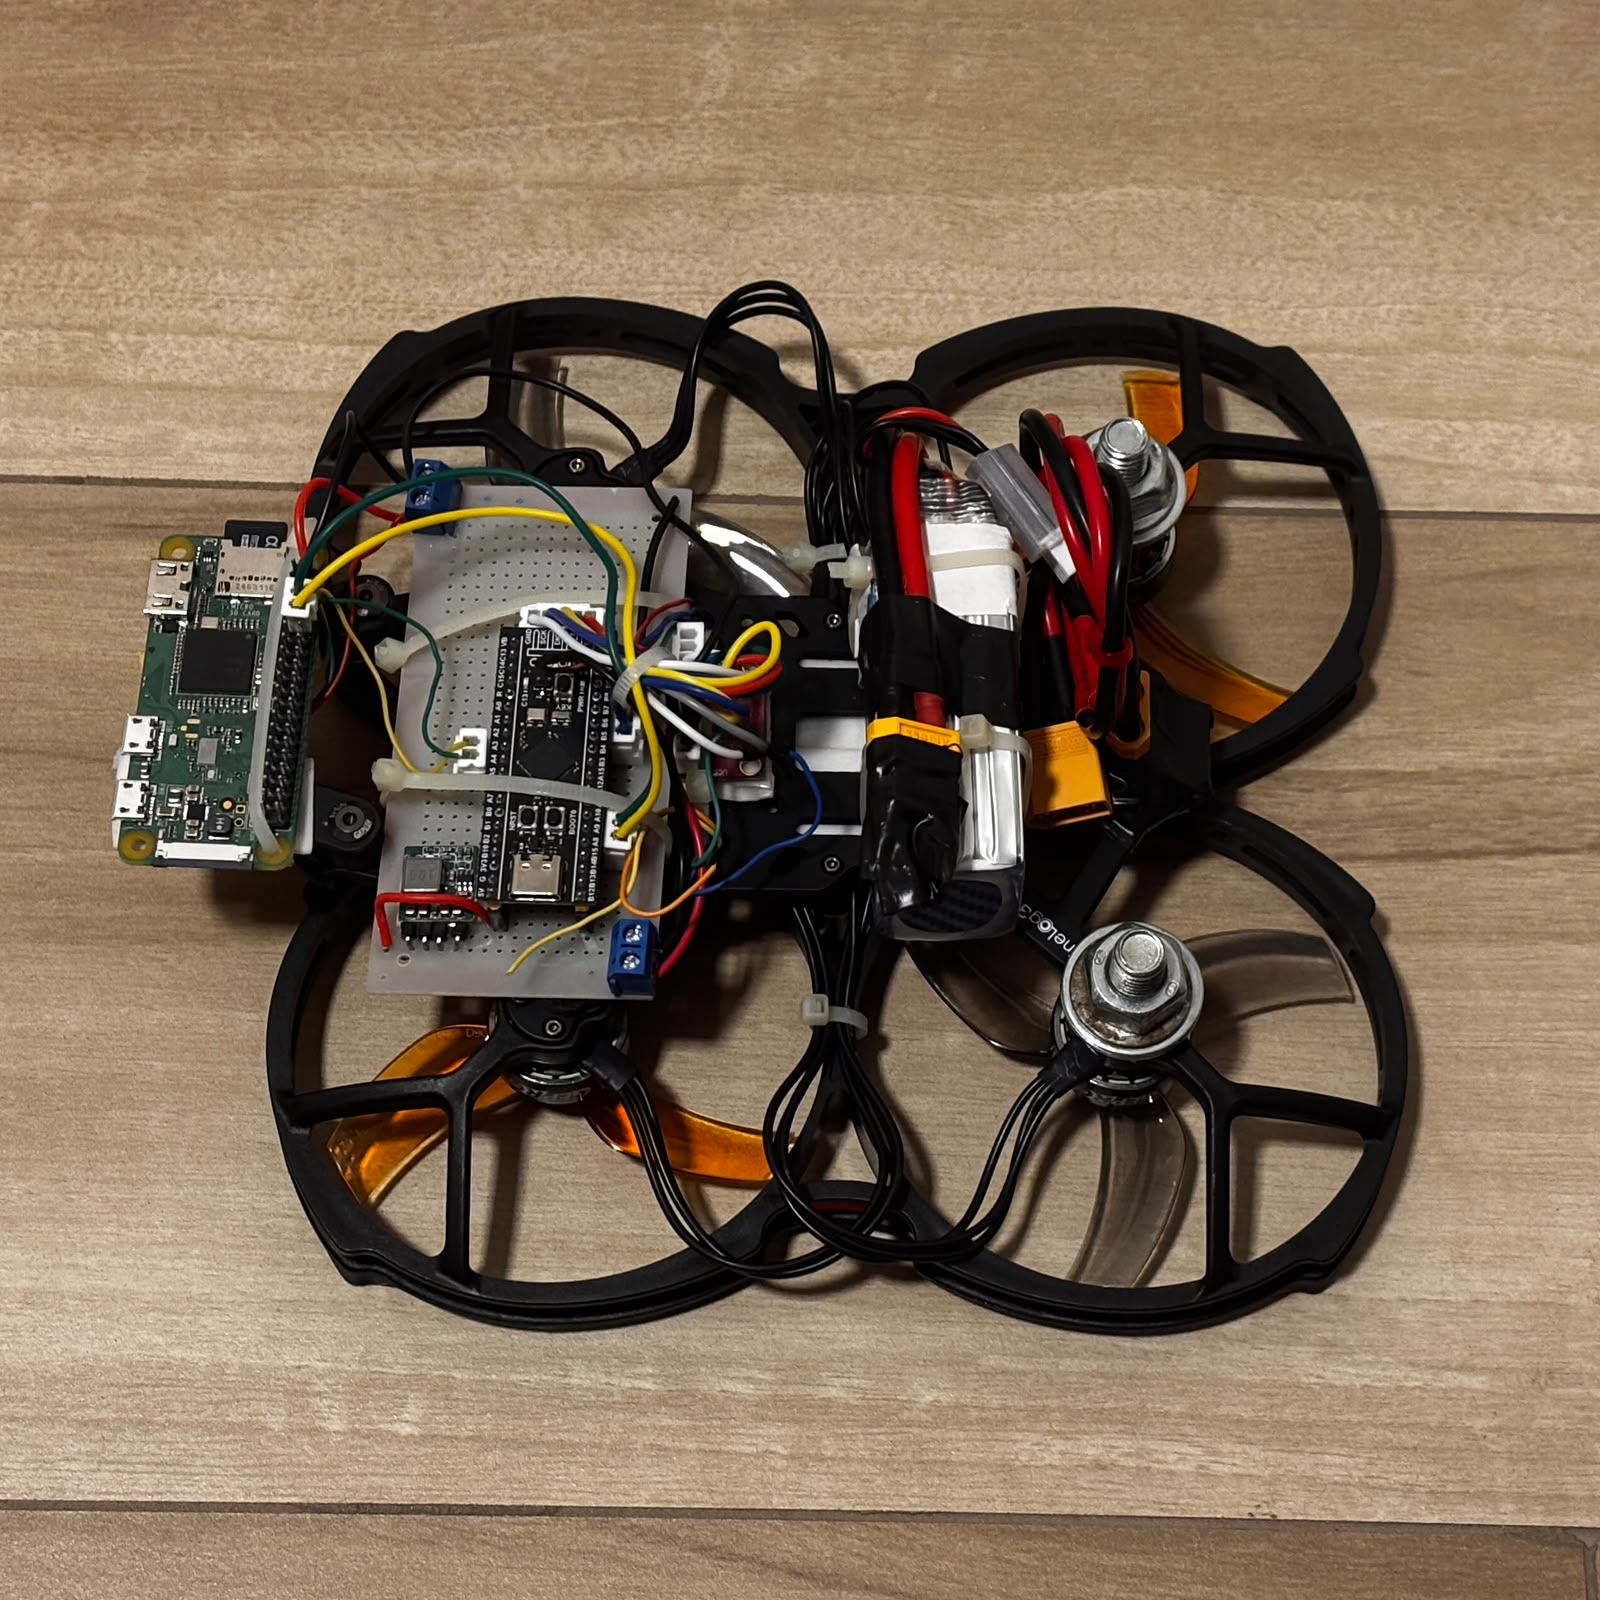
\includegraphics[width=\linewidth,height=4.4cm,keepaspectratio]{images/hardware/prototipo/drone_de_cima.jpeg}
        \par\smallskip{\footnotesize (e) Vista superior}
    \end{minipage}
    \hfill
    \begin{minipage}[t]{0.31\textwidth}
        \centering
        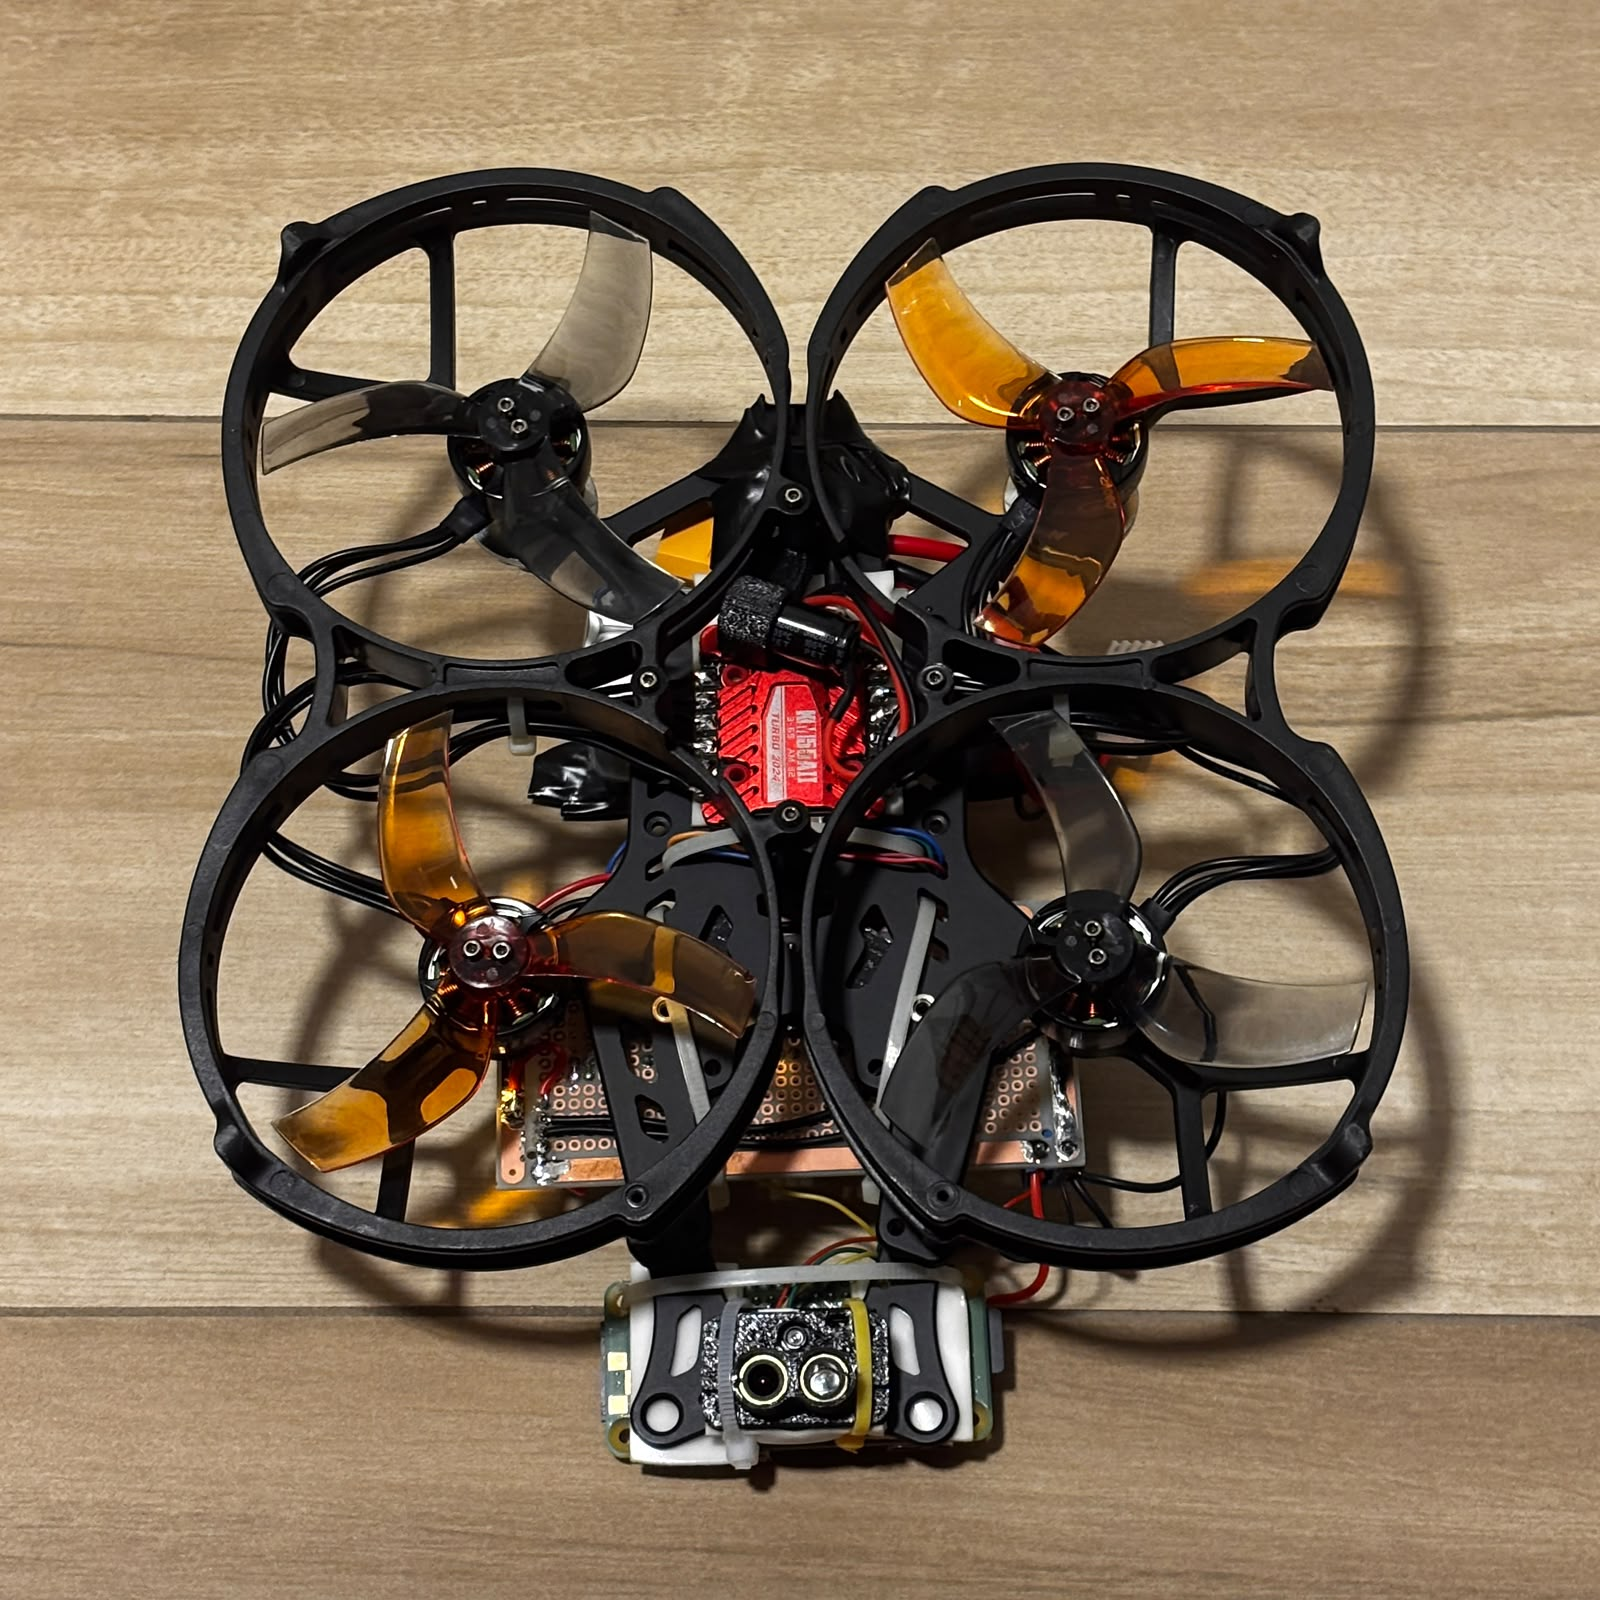
\includegraphics[width=\linewidth,height=4.4cm,keepaspectratio]{images/hardware/prototipo/drone_de_baixo.jpeg}
        \par\smallskip{\footnotesize (f) Vista inferior}
    \end{minipage}
    \par\vspace{0.25cm}
    \footnotesize Fonte: elaborado pelos autores (2026).
\end{figure}

O ambiente de desenvolvimento é apresentado no Quadro~\ref{qua:software}. A versão do projeto e seus arquivos de configuração constituem parte do método, pois permitem reconstruir o ambiente de compilação.

\begin{quadro}[htb]
\centering
\caption{Ambiente de desenvolvimento e versões dos softwares.}
\label{qua:software}
\small
\renewcommand{\arraystretch}{1.3}
\begin{tabular}{
  |
  >{\raggedright\arraybackslash}p{4.5cm}
  |
  >{\raggedright\arraybackslash}p{10.0cm}
  |
}
\hline
\textbf{Elemento} & \textbf{Versão ou configuração} \\
\hline

Sistema Operacional &
Windows 11 Pro 64 bits, versão 10.0.26200, build 26200. \\[4pt]
\hline

STM32CubeIDE &
2.2.0, build 29186\_20260626\_0934 (UTC). \\[4pt]
\hline

STM32CubeMX &
6.18.1-RC2; banco DB.6.0.181 no arquivo \texttt{.ioc} (identificação interna completa preservada). \\[4pt]
\hline

STM32CubeProgrammer &
2.23.0. \\[4pt]
\hline

Compilador &
GNU Tools for STM32 14.3.rel1.20251027-0700\newline
\texttt{arm-none-eabi-gcc} 14.3.1. \\[4pt]
\hline

Bibliotecas STM32 &
STM32CubeF4 1.28.3\newline
HAL 1.8.5\newline
CMSIS Device 2.6.11\newline
CMSIS Core 5.6.0\newline
FreeRTOS 10.3.1 e CMSIS-RTOS2, registradas no projeto \texttt{DroneController}. \\[4pt]
\hline

MATLAB/Simulink &
MATLAB R2024a. \\[4pt]
\hline

Raspberry Pi &
Raspbian GNU/Linux 13 (trixie), Debian 13.4\newline
kernel 6.18.34+rpt-rpi-v6\newline
Python 3.13.5\newline
\texttt{/dev/serial0}$\rightarrow$\texttt{ttyAMA0}\newline
I$^2$C, SPI e UART habilitados. \\[4pt]
\hline

Ambiente Python no Raspberry Pi &
Ambiente virtual em \texttt{\textasciitilde{}/drone-venv}, criado com \texttt{-{}-system-site-packages}\newline
\texttt{pip} 26.2.1\newline
\texttt{pyserial} 3.5\newline
\texttt{pymavlink} 2.4.49\newline
\texttt{fastcrc} 0.3.6\newline
\texttt{lxml} 5.4.0\newline
Validado com abertura de \texttt{/dev/serial0} a 115200 8N1 e empacotamento/leitura de mensagem \textit{HEARTBEAT} MAVLink 2. \\
\hline
\end{tabular}
\par\vspace{0.2cm}
\footnotesize Fonte: elaborado pelos autores (2026), a partir de inspeção do ambiente de desenvolvimento e do projeto \texttt{DroneController} em 06 set. 2026.
\end{quadro}

O projeto STM32 inicializa GPIO, DMA, TIM4, I$^2$C2, USART1, USART2, SPI1 e FreeRTOS por meio de CMSIS-RTOS2. A rastreabilidade do \textit{firmware} é mantida por arquivos \texttt{.ioc}, identificação de versão, instruções de compilação e registros de \textit{build}.

\section{PROCEDIMENTO DE DESENVOLVIMENTO}\label{sec:procedimento_desenvolvimento}

O desenvolvimento é organizado em três frentes complementares: modelagem e simulação do sistema, implementação embarcada com comunicação entre camadas e planejamento de rotas. Essa sequência permite relacionar o modelo matemático, os sinais disponíveis no protótipo e os comandos enviados aos atuadores antes da realização dos ensaios.

\subsection{Modelagem e projeto do controle}\label{subsec:modelagem_projeto_controle}

A modelagem e simulação do sistema consiste em aplicar técnicas de controle partindo do modelo não linear apresentado no Capítulo~\ref{cap_revisao}. Para isso, é necessário parametrizar o sistema, aplicar a linearização em torno do ponto de voo estacionário e projetar o controlador LQG. A validação do modelo é realizada por simulação no MATLAB/Simulink, comparando a resposta do modelo linearizado com a planta não linear e verificando a robustez frente a variações de parâmetros e perturbações. 

\subsubsection{Parametrização do modelo}\label{subsubsec:paremetrizacao_modelo}

Os parâmetros físicos foram obtidos de diferentes formas: alguns foram medidos diretamente, outros foram obtidos e aproximados através de análises de dados e os restantes foram estimados a partir de medições indiretas. A massa do quadricóptero foi medida com uma balança de precisão, enquanto o centro de massa foi determinado por meio de um método de equilíbrio. O momento de inércia foi estimado utilizando o método de decomposição analítica. As características dos motores e hélices foram obtidas através de testes de bancada.

Utilizando uma balança e medindo as dimensões físicas do chassis do drone, foi obtido os seguintes parâmetros do Quadro~\ref{qua:parametros_chassis}.

\begin{quadro}[H]
\centering
\caption{Parâmetros físicos e geométricos do chassi.}
\label{qua:parametros_chassis}
\small
\renewcommand{\arraystretch}{1.3}
\begin{tabular}{
  |
  >{\raggedright\arraybackslash}p{6.8cm}
  |
  >{\centering\arraybackslash}p{2.5cm}
  |
  >{\raggedright\arraybackslash}p{3.5cm}
  |
}
\hline
\textbf{Parâmetro} & \textbf{Variável} & \textbf{Valor} \\
\hline

Massa do corpo central (sem motores) & $M_d$ & 0,463~kg \\[4pt]
\hline

Massa de cada motor & $M_m$ & 0,022~kg \\[4pt]
\hline

Massa total da aeronave & $M$ & 0,551~kg \\[4pt]
\hline

Distância do centro de massa ao motor & $l$ & 0,142~m \\[4pt]
\hline

Comprimento do corpo central & $a$ & 0,104~m \\[4pt]
\hline

Largura do corpo central & $b$ & 0,104~m \\[4pt]
\hline

Altura do corpo central & $c$ & 0,050~m \\[4pt]
\hline

\end{tabular}
\par\vspace{0.2cm}
\footnotesize Fonte: elaborado pelos autores (2026).
\end{quadro}

Para a determinação dos momentos de inércia, empregou-se o método de decomposição analítica proposto por \citeonline{bouabdallah2007}. A decomposição analítica consiste em decompor o quadricóptero em partes, calcular os momentos de inércia de cada parte e somá-los para obter o momento de inércia total. O Quadro~\ref{qua:parametros_inerciais} apresenta os valores obtidos.

\begin{quadro}[H]
\centering
\caption{Parâmetros inerciais do chassi.}
\label{qua:parametros_inerciais}
\small
\renewcommand{\arraystretch}{1.3}
\begin{tabular}{
  |
  >{\raggedright\arraybackslash}p{6.8cm}
  |
  >{\centering\arraybackslash}p{2.5cm}
  |
  >{\raggedright\arraybackslash}p{3.5cm}
  |
}
\hline
\textbf{Parâmetro} & \textbf{Variável} & \textbf{Valor} \\
\hline

Momento de inércia total no eixo x & $I_{xx}$ & 0,00051~kg.m² \\[4pt]
\hline

Momento de inércia total no eixo y & $I_{yy}$ & 0,00051~kg.m² \\[4pt]
\hline

Momento de inércia total no eixo z & $I_{zz}$ & 0,00083~kg.m² \\[4pt]
\hline

\end{tabular}
\par\vspace{0.2cm}
\footnotesize Fonte: elaborado pelos autores (2026).
\end{quadro}

Por fim, os parâmetros aerodinâmicos foram obtidos experimentalmente por meio de ensaios em bancada. A configuração experimental consistiu em uma balança digital invertida, fixada a uma estrutura de suporte e com o prato de pesagem desinstalado, conforme ilustrado na Figura \ref{fig:bancada_teste}. O conjunto propulsor, equipado com os motores GEPRC SPEEDX2 2105.5, também foi montado de forma invertida, procedendo-se com a calibração de tara da balança. O consumo elétrico foi monitorado por meio de um multímetro acoplado a uma fonte de alimentação chaveada. Durante os ensaios, registraram-se o empuxo estático, a corrente consumida e a rotação angular dos motores em função do incremento do comando digital via protocolo DShot.

\begin{figure}[H]
    \centering
    \caption{Bancada de teste de empuxo dos motores.}
    \label{fig:bancada_teste}
    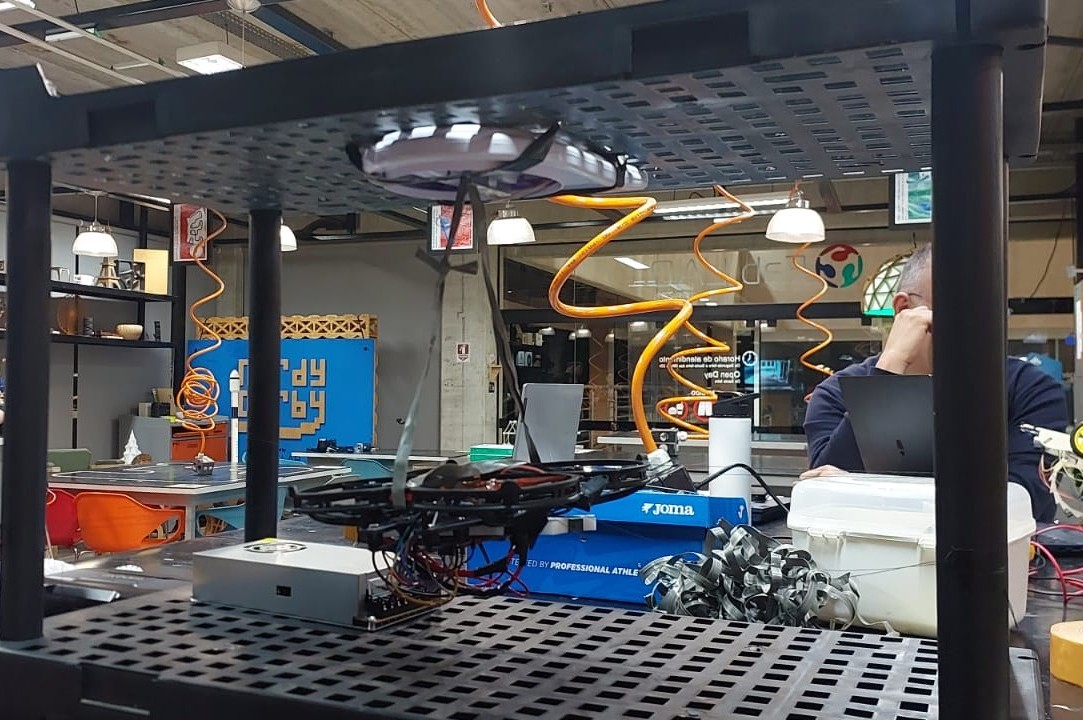
\includegraphics[width=0.85\textwidth]{images/metodologia/bancada_testes.jpeg}
    \par\vspace{0.2cm}
    \footnotesize Fonte: elaborado pelos autores (2026).
\end{figure}

Para determinar as constantes aerodinâmicas a partir dos dados brutos, utilizaram-se abordagens distintas para o empuxo e para o torque. A força de empuxo estático foi modelada pela equação física $T = K_t \omega^2$. Os dados coletados pela balança em gramas-força foram convertidos para Newtons ($1\,\text{gf} \approx 0{,}00981\,\text{N}$) e o coeficiente de empuxo ($K_t$) foi obtido por meio de regressão linear (método dos mínimos quadrados) utilizando a biblioteca \textit{SciPy} em Python, ajustando-se a curva teórica aos pontos experimentais.

Na ausência de um dinamômetro torcional na bancada, o coeficiente de torque ($K_q$) foi estimado de forma indireta por meio do princípio da conservação de potência em máquinas elétricas \cite{chapman2013}. Sabendo que a potência mecânica no eixo do motor é dada por $P_{mec} = \tau \omega$ (com $\tau = K_q \omega^2$) e a potência elétrica ativa consumida é $P_{ele} = V I$, a relação de transferência de energia assume a forma $K_q \omega^3 = \eta V I$, onde $V$ é a tensão da bateria, $I$ a corrente medida e $\eta$ a eficiência eletromecânica do motor \textit{brushless} (BLDC). Como motores de multirrotores operam com perdas aerodinâmicas e térmicas expressivas sob carga \cite{quan2017}, assumiu-se uma eficiência conservadora de $65\%$ ($\eta = 0{,}65$). A partir dessa formulação, calculou-se o valor de $K_q$ ponto a ponto para o regime estabilizado (acima de $100\,\text{rad/s}$) e adotou-se a sua média aritmética.

A Figura \ref{fig:curvas_aerodinamicas} ilustra os pontos coletados experimentalmente e a curva ajustada para o empuxo. Devido a limitações de fornecimento de corrente da fonte chaveada utilizada na bancada, a coleta de dados foi restrita à velocidade angular máxima de aproximadamente $1200\,\text{rad/s}$. A resposta aerodinâmica para rotações superiores é representada por uma linha de tendência, consistindo na extrapolação do modelo quadrático ajustado.

\begin{figure}[H]
\centering
\caption{Curva experimental de empuxo em função da velocidade angular.}
\label{fig:curvas_aerodinamicas}
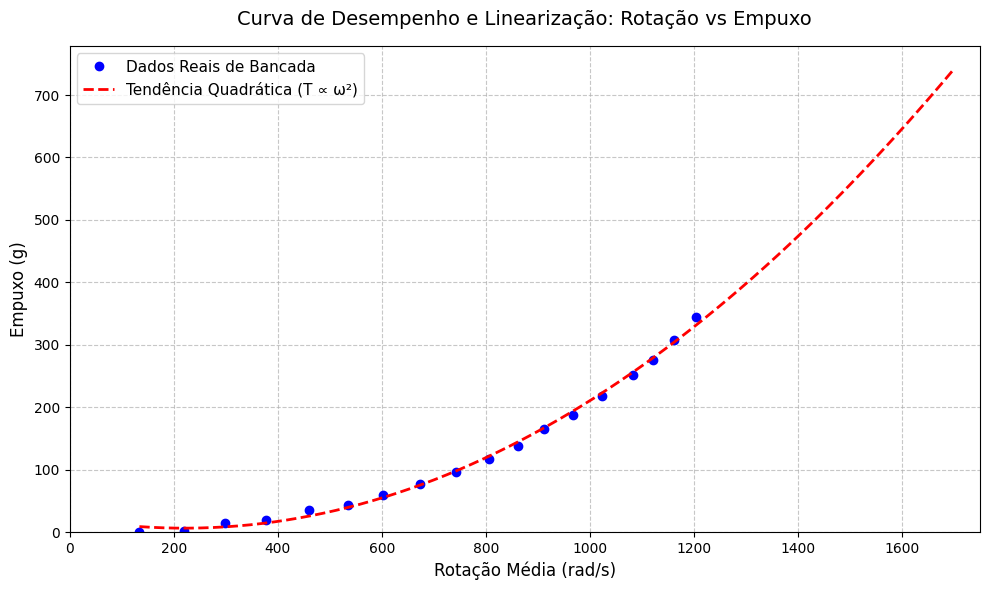
\includegraphics[width=0.75\textwidth]{images/metodologia/empuxo_x_rotacao.png}
\vspace{0.2cm}
\par\footnotesize Fonte: elaborado pelos autores (2026).
\end{figure}

Os valores finais extraídos da regressão, fundamentais para a modelagem dinâmica do sistema no espaço de estados, estão sintetizados no Quadro \ref{qua:parametros_aerodinamicos}.

\begin{quadro}[H]
\centering
\caption{Parâmetros aerodinâmicos das hélices.}
\label{qua:parametros_aerodinamicos}
\small
\renewcommand{\arraystretch}{1.3}
\begin{tabular}{|>{\raggedright\arraybackslash}p{4.8cm}|>{\centering\arraybackslash}p{2.5cm}|>{\centering\arraybackslash}p{5.5cm}|}
\hline
\textbf{Parâmetro} & \textbf{Variável} & \textbf{Valor} \\
\hline
Coeficiente de empuxo & $K_t$ & $2{,}09 \times 10^{-6} \mathrm{\, N\cdot s^2/rad^2}$ \\[4pt]
\hline
Coeficiente de torque & $K_q$ & $2{,}61 \times 10^{-5} \mathrm{\, N\cdot m\cdot s^2/rad^2}$ \\[4pt]
\hline
\end{tabular}
\par\vspace{0.2cm}
\footnotesize Fonte: elaborado pelos autores (2026).
\end{quadro}

\subsubsection{Linearização do sistema}\label{subsubsec:linearizacao_sistema}

Conforme apresentado no Capítulo~\ref{cap_revisao}, a linearização do modelo não linear é realizada em torno do ponto de equilíbrio de voo estacionário (\textit{hover}), onde $\phi_0 = \theta_0 = \psi_0 = 0\text{~rad}$, as velocidades lineares e angulares são nulas e o empuxo total equilibra o peso da aeronave ($T_0 = M g \approx 5{,}4\text{~N}$). Como os quatro conjuntos propulsores dividem igualmente a sustentação no equilíbrio, a velocidade angular nominal de cada rotor é dada por:

\begin{equation}\label{eq:omega_hover}
\omega_0 = \sqrt{\frac{M g}{4 K_t}} = \sqrt{\frac{0,551 \times 9{,}81}{4 \times 2{,}09 \times 10^{-6}}} \approx 804~\text{rad/s}.
\end{equation}

\noindent em que $K_t$ é o coeficiente de empuxo e $K_q$ é o coeficiente de torque aerodinâmico das hélices.

Definindo o vetor de estados $\mathbf{x} \in \mathbb{R}^{12}$ e tomando diretamente as velocidades de rotação dos quatro motores como o vetor de entradas $\mathbf{u} \in \mathbb{R}^{4}$:

\begin{equation}\label{eq:vetores_x_u_motores}
\begin{aligned}
\mathbf{x} &= \begin{bmatrix} x & y & z & \phi & \theta & \psi & \dot{x} & \dot{y} & \dot{z} & p & q & r \end{bmatrix}^T, \\
\mathbf{u} &= \begin{bmatrix} \omega_1 & \omega_2 & \omega_3 & \omega_4 \end{bmatrix}^T,
\end{aligned}
\end{equation}

\noindent aplica-se a expansão em série de Taylor de primeira ordem. A avaliação da matriz Jacobiana de estados $\mathbf{A} = \left.\partial \mathbf{f}/\partial \mathbf{x}\right|_{(\mathbf{x}_0,\mathbf{u}_0)}$ resulta na matriz esparsa $12 \times 12$:

\begin{equation}\label{eq:matriz_A_linear}
\setlength{\arraycolsep}{3.5pt}
\mathbf{A} = 
\begin{bmatrix}
0 & 0 & 0 & 0 & 0 & 0 & 1 & 0 & 0 & 0 & 0 & 0 \\
0 & 0 & 0 & 0 & 0 & 0 & 0 & 1 & 0 & 0 & 0 & 0 \\
0 & 0 & 0 & 0 & 0 & 0 & 0 & 0 & 1 & 0 & 0 & 0 \\
0 & 0 & 0 & 0 & 0 & 0 & 0 & 0 & 0 & 1 & 0 & 0 \\
0 & 0 & 0 & 0 & 0 & 0 & 0 & 0 & 0 & 0 & 1 & 0 \\
0 & 0 & 0 & 0 & 0 & 0 & 0 & 0 & 0 & 0 & 0 & 1 \\
0 & 0 & 0 & 0 & -g & 0 & 0 & 0 & 0 & 0 & 0 & 0 \\
0 & 0 & 0 & g & 0 & 0 & 0 & 0 & 0 & 0 & 0 & 0 \\
0 & 0 & 0 & 0 & 0 & 0 & 0 & 0 & 0 & 0 & 0 & 0 \\
0 & 0 & 0 & 0 & 0 & 0 & 0 & 0 & 0 & 0 & 0 & 0 \\
0 & 0 & 0 & 0 & 0 & 0 & 0 & 0 & 0 & 0 & 0 & 0 \\
0 & 0 & 0 & 0 & 0 & 0 & 0 & 0 & 0 & 0 & 0 & 0
\end{bmatrix}.
\end{equation}

Para a matriz de entrada $\mathbf{B} = \left.\partial \mathbf{f}/\partial \mathbf{u}\right|_{(\mathbf{x}_0,\mathbf{u}_0)}$, considera-se a geometria do chassi em configuração ``X'', na qual os braços formam ângulos de $45^\circ$ com os eixos principais do corpo, resultando em um braço de alavanca efetivo de $l\frac{\sqrt{2}}{2}$ para rolagem e arfagem. Derivando os esforços propulsivos quadráticos ($T_i = K_t\omega_i^2$ e $\tau_{\psi,i} = K_q\omega_i^2$) em torno da rotação de equilíbrio $\omega_0$, obtém-se $\partial T_i/\partial\omega_i = 2K_t\omega_0$, o que conduz à matriz $\mathbf{B} \in \mathbb{R}^{12\times 4}$:

\begin{equation}\label{eq:matriz_B_linear}
\setlength{\arraycolsep}{4pt}
\mathbf{B} = 
\begin{bmatrix}
0 & 0 & 0 & 0 \\
0 & 0 & 0 & 0 \\
0 & 0 & 0 & 0 \\
0 & 0 & 0 & 0 \\
0 & 0 & 0 & 0 \\
0 & 0 & 0 & 0 \\
0 & 0 & 0 & 0 \\
0 & 0 & 0 & 0 \\[2pt]
-\dfrac{2 K_t \omega_0}{M} & -\dfrac{2 K_t \omega_0}{M} & -\dfrac{2 K_t \omega_0}{M} & -\dfrac{2 K_t \omega_0}{M} \\[10pt]
\dfrac{\sqrt{2} l K_t \omega_0}{I_{xx}} & -\dfrac{\sqrt{2} l K_t \omega_0}{I_{xx}} & -\dfrac{\sqrt{2} l K_t \omega_0}{I_{xx}} & \dfrac{\sqrt{2} l K_t \omega_0}{I_{xx}} \\[10pt]
\dfrac{\sqrt{2} l K_t \omega_0}{I_{yy}} & \dfrac{\sqrt{2} l K_t \omega_0}{I_{yy}} & -\dfrac{\sqrt{2} l K_t \omega_0}{I_{yy}} & -\dfrac{\sqrt{2} l K_t \omega_0}{I_{yy}} \\[10pt]
-\dfrac{2 K_q \omega_0}{I_{zz}} & \dfrac{2 K_q \omega_0}{I_{zz}} & -\dfrac{2 K_q \omega_0}{I_{zz}} & \dfrac{2 K_q \omega_0}{I_{zz}}
\end{bmatrix}.
\end{equation}

\subsubsection{Projeto do controlador LQG}\label{subsubsec:projeto_controlador_lqg}

Com o modelo linearizado definido pelas matrizes $\mathbf{A}$ e $\mathbf{B}$, procede-se à síntese do controlador Linear Quadrático Gaussiano (LQG), estruturada em duas etapas independentes conforme o princípio da separação apresentado na Seção~\ref{subsec:lqg}: o cálculo do ganho de realimentação de estados via LQR e o projeto do observador estocástico via Filtro de Kalman.

Para a etapa de regulação (LQR), as matrizes de ponderação de estados $\mathbf{Q} \in \mathbb{R}^{12\times 12}$ e de esforço de controle $\mathbf{R}_{\mathrm{lqr}} \in \mathbb{R}^{4\times 4}$ foram definidas como matrizes diagonais:

\begin{equation}\label{eq:matrizes_Q_R_metodo}
\begin{aligned}
\mathbf{Q} &= \operatorname{diag}\left(q_x,\, q_y,\, q_z,\, q_\phi,\, q_\theta,\, q_\psi,\, q_{\dot{x}},\, q_{\dot{y}},\, q_{\dot{z}},\, q_p,\, q_q,\, q_r\right), \\
\mathbf{R}_{\mathrm{lqr}} &= \operatorname{diag}\left(r_1,\, r_2,\, r_3,\, r_4\right).
\end{aligned}
\end{equation}

Os pesos foram ajustados iterativamente em ambiente de simulação no software MATLAB, priorizando a rápida estabilização das variáveis de atitude ($\phi, \theta, \psi$) e de altitude ($z$), enquanto as ponderações em $\mathbf{R}_{\mathrm{lqr}}$ foram dimensionadas de modo a evitar a saturação prematura dos comandos de velocidade angular enviados aos quatro motores. A partir das matrizes $(\mathbf{A}, \mathbf{B}, \mathbf{Q}, \mathbf{R}_{\mathrm{lqr}})$, obteve-se a matriz de ganho ótimo $\mathbf{K} \in \mathbb{R}^{4\times 12}$.

Na etapa de estimação de estados, a matriz de saída $\mathbf{C}$ foi definida com base nas variáveis efetivamente mensuradas pelo conjunto de sensores da aeronave: a altitude no eixo $z$ e as velocidades lineares nos eixos $x$ e $y$, fornecidas pelo módulo óptico/ToF MTF-01, bem como os ângulos de Euler e as velocidades angulares, obtidos pela unidade de medição inercial BNO08X. Por simplificação de projeto, a matriz de transmissão direta $\mathbf{D}$ foi considerada nula.

A matriz de ruído de processo $\mathbf{Q}_w$ foi ajustada através de simulações, considerando a dinâmica do sistema e a incerteza nos modelos de motores e hélices e a matriz de ruído de medição $\mathbf{R}_v$ foi definida através de testes experimentais, registrando a variância das leituras dos sensores em condições estáticas e em voo:

\begin{equation}\label{eq:matrizes_kalman_metodo}
\mathbf{Q}_w = \operatorname{diag}\left(\sigma_{w,1}^2, \dots, \sigma_{w,12}^2\right), \qquad
\mathbf{R}_v = \operatorname{diag}\left(\sigma_{v,1}^2, \dots, \sigma_{v,p}^2\right).
\end{equation}

Por fim, o acoplamento do estimador com o regulador forma a malha fechada LQG conforme a Figura~\ref{fig:LQRController}. A cada ciclo de controle, o Filtro de Kalman processa as leituras ruidosas $\mathbf{y}$ e a ação de controle anterior para gerar o vetor de estados estimados $\hat{\mathbf{x}}$. O comando total de velocidade angular aplicado aos motores é então calculado somando-se a ação corretiva do LQR à velocidade nominal de equilíbrio $\mathbf{u}_0 = [\omega_0,\, \omega_0,\, \omega_0,\, \omega_0]^{\mathrm{T}}$:

\begin{equation}\label{eq:comando_final_motores}
\mathbf{u} = \mathbf{u}_0 - \mathbf{K}\left(\hat{\mathbf{x}} - \mathbf{x}_{\mathrm{ref}}\right),
\end{equation}

\noindent sendo o vetor resultante $\mathbf{u}$ submetido a um bloco de saturação que restringe as rotações ao intervalo físico operacional dos propulsores $[\omega_{\min},\, \omega_{\max}]$.

\begin{figure}[H]
    \centering
    \caption{Sistema controlador LQG.}
    \label{fig:LQRController}
    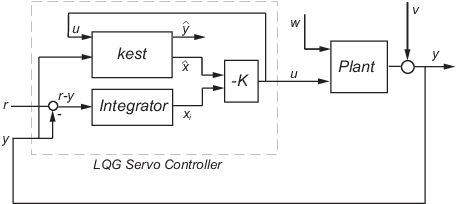
\includegraphics[width=0.8\textwidth]{images/metodologia/LQGController.png}
    \par\vspace{0.2cm}
    \footnotesize Fonte: \citeonline{mathworkslqg}.
\end{figure}

\subsubsection{Comparação entre o sistema linear e o sistema não linear}\label{subsubsec:comp_linear_nao_linear}
Para validar os ganhos obtidos pelo LQR e pelo Filtro de Kalman, foi realizada uma simulação comparativa entre o sistema linearizado e o sistema não linear através do software MATLAB/Simulink. A simulação envolveu a aplicação de perturbações iniciais e a análise da resposta do sistema em termos de estabilidade, tempo de assentamento e overshoot.

\subsection{Implementação embarcada e comunicação}\label{subsec:implementacao_embarcada}

O \textit{firmware} é gerado e compilado com as versões indicadas no Quadro~\ref{qua:software}. FreeRTOS é utilizado para estruturar tarefas e sincronização; consequentemente, o trabalho caracteriza o \textit{firmware} como uma aplicação embarcada com sistema operacional de tempo real. A prioridade e o período de cada tarefa são registrados no código e no relatório de execução.

O barramento I$^2$C2 foi configurado em 400~kHz para a IMU, com PB10 como SCL, PB3 como SDA, PB4 como entrada de interrupção e PB5 como reset. Os canais PB6--PB9 de TIM4 foram reservados para os quatro sinais de motores. A geração DShot por temporizador e DMA é validada primeiro por analisador lógico ou osciloscópio, sem hélices, antes de qualquer ligação aos motores. DShot transmite um valor de \textit{throttle}, um bit de solicitação de telemetria e CRC em uma palavra de 16 bits; o protocolo e seus limites dependem da configuração do ESC \cite{betaflightdshot}.

O ESC utiliza firmware AM32, cuja documentação indica ferramentas de configuração e atualização e suporte ao microcontrolador AT32F421 \cite{am32manual}. Antes de qualquer atualização, os quatro canais são lidos com hélices removidas, registrando-se as versões de \textit{firmware}, \textit{target}, \textit{bootloader} e os parâmetros exportáveis. A identificação da versão instalada é evidência de reprodutibilidade e não pode ser substituída pela versão mais recente disponível na Internet.

% Comunicação Raspberry Pi <-> STM32: enlace, DroneLink, comandos e ensaios
% ============================================================================
% MATERIAIS E MÉTODOS — comunicação entre o Raspberry Pi e o STM32 (DroneLink)
% Chamado em partes/textuais/metodologias.tex, depois de "Implementação
% embarcada e comunicação".
% ============================================================================

\subsection{Comunicação entre o computador de missão e o controlador de voo}\label{subsec:metodo_comunicacao}

A comunicação entre o Raspberry Pi (computador de missão) e o STM32 (controlador de voo) segue o DroneLink, protocolo de aplicação desenvolvido neste trabalho sobre o enquadramento MAVLink 2 (Seção~\ref{subsec:mavlink}). A divisão de responsabilidades é a seguinte: o Raspberry Pi decide \textbf{o que} fazer, isto é, a ordem dos pontos e o próximo objetivo; o STM32 decide \textbf{como} e \textbf{se} fazer, validando cada pedido, executando-o com o controlador LQG e mantendo o VANT seguro mesmo que o Raspberry Pi falhe.

\subsubsection{Enlace físico e ambiente do Raspberry Pi}\label{subsubsec:com_enlace}

No enlace físico entre Raspberry Pi e STM32, a configuração adotada é UART \textit{full-duplex} em lógica de 3,3~V, 115200~bit/s, 8N1 e sem controle de fluxo. O GPIO14/TXD do Raspberry Pi, pino físico 8, liga-se ao PA10/USART1\_RX do STM32; o PA9/USART1\_TX do STM32 liga-se ao GPIO15/RXD do Raspberry Pi, pino físico 10; e o GND comum é obrigatório. No Raspberry Pi, a interface serial está exposta em \texttt{/dev/serial0}, apontando para \texttt{ttyAMA0}, com \texttt{enable\_uart=1}, Bluetooth desabilitado pelo \textit{overlay} \texttt{disable-bt} e console serial desativado, de modo que a UART fique dedicada à comunicação com o controlador de voo.

O software do Raspberry Pi foi desenvolvido em Python 3.13.5, com as bibliotecas \texttt{pyserial} 3.5, \texttt{pymavlink} 2.4.49 e \texttt{numpy} 2.2.4, no Raspberry Pi OS 13 (ARMv6). Sua preparação foi verificada pela abertura da interface serial e pela recepção das mensagens periódicas do STM32. O código e sua organização estão disponíveis no repositório apresentado no Apêndice~\ref{ap:repositorio}.

\subsubsection{Construção do dialeto DroneLink}\label{subsubsec:com_dialeto}

O protocolo é definido em um único arquivo, \texttt{protocol/drone\_controller.xml}, que inclui o \texttt{common.xml} do MAVLink e acrescenta as mensagens próprias do projeto, com identificadores a partir de 51000, faixa não usada pelo \texttt{common.xml}. Desse arquivo são gerados os dois lados do enlace: os \textit{headers} C do STM32, pelo gerador oficial \texttt{mavgen}, e o módulo Python do Raspberry Pi, pela biblioteca \texttt{pymavlink}, que o regera automaticamente sempre que o XML muda. A geração a partir da mesma definição mantém a estrutura das mensagens consistente entre os dois lados, e o \texttt{CRC\_EXTRA} auxilia na detecção de definições incompatíveis.

O STM32 usa o \textit{System ID}~1 e o \textit{Component ID}~1 (piloto automático), e o Raspberry Pi, o mesmo \textit{System ID} com o \textit{Component ID}~191 (computador de bordo). O STM32 só processa mensagens com essa origem e com o destino indicado nos campos \texttt{target\_system} e \texttt{target\_component} de cada mensagem; as demais são ignoradas. As mensagens utilizadas estão no Quadro~\ref{qua:dronelink_mensagens}.

\begin{quadro}[H]
    \centering
    \caption{Mensagens do DroneLink.}
    \label{qua:dronelink_mensagens}
    \footnotesize
    \renewcommand{\arraystretch}{1.25}
    \setlength{\tabcolsep}{3pt}
    \begin{tabular}{|>{\raggedright\arraybackslash}p{4.2cm}|>{\centering\arraybackslash}p{1.1cm}|>{\centering\arraybackslash}p{1.1cm}|>{\raggedright\arraybackslash}p{1.6cm}|>{\raggedright\arraybackslash}p{5.4cm}|}
        \hline
        \textbf{Mensagem} & \textbf{De} & \textbf{Para} & \textbf{Taxa} & \textbf{Função} \\
        \hline
        \multicolumn{5}{|l|}{\textbf{Padrão (\texttt{common.xml})}} \\
        \hline
        \texttt{HEARTBEAT} & Pi & STM32 & 4~Hz & Presença do computador de missão. \\
        \hline
        \texttt{HEARTBEAT} & STM32 & Pi & 2~Hz & Estado de voo e indicação de armado. \\
        \hline
        \texttt{COMMAND\_\allowbreak LONG} & Pi & STM32 & Por pedido & Solicitação de armar ou desarmar. \\
        \hline
        \texttt{COMMAND\_\allowbreak ACK} & STM32 & Pi & Por resposta & Aceite ou recusa do comando. \\
        \hline
        \texttt{PARAM\_\allowbreak *} & Pi & STM32 & Por pedido & Consulta ou alteração de parâmetros. \\
        \hline
        \texttt{PARAM\_\allowbreak VALUE} & STM32 & Pi & Por resposta & Valor efetivamente adotado. \\
        \hline
        \texttt{ATTITUDE, LOCAL\_\allowbreak POSITION\_\allowbreak NED} & STM32 & Pi & 5~Hz & Atitude e posição estimadas. \\
        \hline
        \texttt{SYS\_\allowbreak STATUS, STATUSTEXT} & STM32 & Pi & Periódica / por evento & Estado do sistema e avisos; bateria quando disponível. \\
        \hline
        \texttt{TIMESYNC} & Pi & STM32 & Por pedido & Solicitação de sincronização dos relógios. \\
        \hline
        \texttt{TIMESYNC} & STM32 & Pi & Por resposta & Horário local para sincronização. \\
        \hline
        \multicolumn{5}{|l|}{\textbf{Próprias do DroneLink}} \\
        \hline
        \texttt{DRONE\_\allowbreak PROTOCOL\_\allowbreak INFO} & STM32 & Pi & 1~Hz & Versão, identidade de boot e capacidades. \\
        \hline
        \texttt{DRONE\_\allowbreak LEG\_\allowbreak COMMAND} & Pi & STM32 & Por pedido & Solicitação de um trecho. \\
        \hline
        \texttt{DRONE\_\allowbreak LEG\_\allowbreak ACK} & STM32 & Pi & Por resposta & Situação e resultado do trecho. \\
        \hline
        \texttt{DRONE\_\allowbreak LEG\_\allowbreak CANCEL} & Pi & STM32 & Por pedido & Cancelamento do trecho. \\
        \hline
        \texttt{DRONE\_\allowbreak CONTROL\_\allowbreak LEASE} & Pi & STM32 & 5~Hz & Autorização válida por 1~s. \\
        \hline
        \texttt{DRONE\_\allowbreak GAIN\_\allowbreak ROW, DRONE\_\allowbreak GAIN\_\allowbreak COMMIT} & Pi & STM32 & Por ajuste & Envio e aplicação dos ganhos do LQG. \\
        \hline
        \texttt{DRONE\_\allowbreak GAIN\_\allowbreak ACK} & STM32 & Pi & Por resposta & Resultado do ajuste dos ganhos. \\
        \hline
        \texttt{DRONE\_\allowbreak CTRL\_\allowbreak DEBUG} & STM32 & Pi & Por ajuste & Medições, estimativas, comandos e referências. \\
        \hline
    \end{tabular}
    \par\vspace{0.2cm}
    \footnotesize Fonte: elaborado pelos autores (2026).
\end{quadro}

\subsubsection{Trecho de missão (\textit{leg})}\label{subsubsec:com_trecho}

Um trecho é uma ação solicitada pelo Raspberry Pi ao STM32, como decolar, girar, deslocar-se, manter a posição ou pousar. O pedido contém a ação, o alvo, os limites de execução e os identificadores que o associam à missão e à resposta correspondente.

Antes de aceitar o pedido, o STM32 verifica sua compatibilidade com o estado do veículo, os limites de movimento e as condições de comunicação e autorização. Se o pedido for recusado, o controlador informa o motivo por meio dos códigos apresentados no Quadro~\ref{qua:dronelink_motivos}.

As respostas são enviadas em campos numéricos da mensagem \texttt{DRONE\_LEG\_ACK}, indicando se a operação está em andamento, foi concluída, recusada ou falhou. Os nomes apresentados no quadro correspondem aos identificadores em inglês definidos pelo protocolo.

Na decolagem e nos trechos de movimento, a conclusão depende de o veículo permanecer no alvo por 1~s, dentro das tolerâncias definidas e com velocidades estimadas baixas. Nos ensaios, foram adotadas tolerâncias de 5~cm para posição e 0,05~rad para guinada, além de limites de 5~cm/s para velocidade linear e 0,1~rad/s para velocidade angular. A confirmação de conclusão é enviada após essa verificação.


\begin{quadro}[H]
    \centering
    \caption{Principais motivos de recusa de um trecho.}
    \label{qua:dronelink_motivos}
    \small
    \renewcommand{\arraystretch}{1.25}
    \begin{tabular}{|>{\raggedright\arraybackslash}p{4.8cm}|>{\raggedright\arraybackslash}p{9cm}|}
        \hline
        \textbf{Motivo} & \textbf{Situação} \\
        \hline
        \texttt{BAD\_STATE} &
        O estado do VANT não permite executar a ação solicitada. \\
        \hline
        \texttt{BUSY} &
        Há outra operação em execução. \\
        \hline
        \texttt{OUT\_OF\_BOUNDS} &
        Algum campo do pedido está fora da faixa permitida. \\
        \hline
        \texttt{STALE\_BOOT} &
        A identidade de inicialização informada não corresponde à atual do STM32. \\
        \hline
        \texttt{SEQUENCE\_ERROR} &
        O índice do trecho não corresponde à sequência esperada. \\
        \hline
        \texttt{OPERATOR\_LEASE\_LOST} &
        A autorização do operador não está ativa. \\
        \hline
        \texttt{LINK\_LOST} &
        O \textit{HEARTBEAT} do Raspberry Pi não é recebido há pelo menos 1~s. \\
        \hline
        \texttt{SENSOR\_UNHEALTHY} &
        Uma condição de sensor necessária à operação não foi atendida. \\
        \hline
        \texttt{ID\_COLLISION} &
        Os mesmos identificadores foram usados em pedidos com conteúdos diferentes. \\
        \hline
    \end{tabular}
    \par\vspace{0.2cm}
    \footnotesize Fonte: elaborado pelos autores (2026).
\end{quadro}

\subsubsection{Idempotência e identidade de \textit{boot}}\label{subsubsec:com_idempotencia}

O Raspberry Pi aguarda até 1~s pela primeira resposta de cada trecho e, se ela não chega, reenvia o mesmo pedido, com os mesmos identificadores, até três vezes. Para que o reenvio seja seguro, o STM32 guarda um histórico circular das 32 últimas transações, com os identificadores e um \textit{hash} do conteúdo. Um pedido repetido recebe a mesma resposta já enviada, sem ser executado de novo, o que implementa a semântica de no máximo uma vez (Seção~\ref{subsec:comunicacao_confiavel}); um pedido com os mesmos identificadores e conteúdo diferente é recusado por colisão de identificador.

A cada inicialização, o STM32 incrementa um contador de \textit{boots} gravado em um registro na memória \textit{flash} externa W25Q64, e o valor é publicado como \texttt{boot\_id}. O Raspberry Pi copia esse valor em todos os pedidos. Se o STM32 reiniciar durante uma missão, os pedidos antigos passam a ser recusados por \textit{boot} desatualizado, impedindo que um comando anterior à reinicialização seja executado. Sem um \texttt{boot\_id} persistente, o STM32 não aceita armar nem executar trechos.

\subsubsection{Supervisão do enlace e da autorização do operador}\label{subsubsec:com_supervisao}

Durante o voo, o STM32 supervisiona o enlace com o Raspberry Pi e a autorização do operador. Em caso de perda, solicita as ações do Quadro~\ref{qua:dronelink_failsafe}: \textit{HOLD}, para manter a posição, ou \textit{LAND}, para pousar.
  

\begin{quadro}[H]
    \centering
    \caption{Ações do STM32 diante da perda do enlace ou da autorização.}
    \label{qua:dronelink_failsafe}
    \small
    \renewcommand{\arraystretch}{1.25}
    \begin{tabular}{|>{\raggedright\arraybackslash}p{7.6cm}|>{\raggedright\arraybackslash}p{6.2cm}|}
        \hline
        \textbf{Condição} & \textbf{Ação solicitada} \\
        \hline
        Sem \textit{HEARTBEAT} do Raspberry Pi por 1~s &
        \textit{Request HOLD}; novos trechos são recusados. \\
        \hline
        Sem \textit{HEARTBEAT} por 2~s e com navegação degradada
        (posição, altura ou atitude inválidas) &
        \textit{Request LAND}. \\
        \hline
        Sem \textit{HEARTBEAT} por 5~s &
        \textit{Request LAND}. \\
        \hline
        Autorização do operador expirada ou retirada &
        \textit{Request HOLD}. \\
        \hline
        Autorização expirada ou retirada por 5~s &
        \textit{Request LAND}. \\
        \hline
    \end{tabular}
    \par\vspace{0.2cm}
    \footnotesize Fonte: elaborado pelos autores (2026), a partir da configuração do protocolo.
\end{quadro}

Essa supervisão vale somente para voos iniciados pelo Raspberry Pi. Voos de bancada comandados pelo console USB do STM32 não dependem do enlace, o que permitiu os ensaios descritos na Seção~\ref{subsubsec:com_ensaios}.

\subsubsection{Implementação no STM32}\label{subsubsec:com_firmware}

No STM32, a comunicação é dividida entre transporte, tratamento do protocolo e telemetria. A USART1 recebe por DMA circular de 512~bytes, e uma tarefa do FreeRTOS processa as mensagens. Na transmissão, respostas de comandos e \textit{HEARTBEAT} têm prioridade sobre a telemetria ainda na fila. Todos os módulos compartilham o contador de sequência MAVLink, necessário à identificação de mensagens ausentes.

O protocolo utiliza o histórico de pedidos e a identidade de inicialização descritos anteriormente. Uma interface de comandos conecta a comunicação ao controle de voo, permitindo que tanto o Raspberry Pi quanto o console USB solicitem ações ao mesmo controlador. A telemetria informa atitude, posição e estado de voo; a altura publicada é medida a partir do chão registrado ao armar, referência também usada na decolagem.

\subsubsection{Ferramenta do Raspberry Pi e comandos do operador}\label{subsubsec:com_comandos}

O programa \texttt{dronectl} permite ao operador executar comandos e missões pelo Raspberry Pi. No modo \texttt{missao}, as instruções podem ser fornecidas pelo terminal ou por arquivo, conforme o Quadro~\ref{qua:dronelink_comandos}.

Por exemplo, durante uma rota, o Raspberry Pi aguarda a confirmação do STM32 antes de avançar ao próximo trecho. Enquanto o trecho está em execução, o controlador informa \texttt{MAV\_RESULT\_IN\_PROGRESS}; ao concluí-lo, envia \texttt{MAV\_RESULT\_ACCEPTED} com progresso de 100\%. Em caso de erro no arquivo ou interrupção pelo operador, o Raspberry Pi solicita o pouso.



\begin{quadro}[H]
    \centering
    \caption{Comandos do operador no modo de missão.}
    \label{qua:dronelink_comandos}
    \footnotesize
    \renewcommand{\arraystretch}{1.25}
    \begin{tabular}{|>{\raggedright\arraybackslash}p{3.6cm}|>{\raggedright\arraybackslash}p{6.2cm}|>{\raggedright\arraybackslash}p{4.1cm}|}
        \hline
        \textbf{Comando} & \textbf{Função} & \textbf{Mensagens enviadas} \\
        \hline
        \texttt{takeoff <cm>} & Arma e sobe até a altura; termina com o VANT estável. & \texttt{COMMAND\_LONG} (armar) e trecho de decolagem \\
        \hline
        \texttt{yaw <graus>} & Gira no lugar; positivo é horário visto de cima. & Trecho de giro \\
        \hline
        \texttt{forward}, \texttt{back}, \texttt{right}, \texttt{left}, \texttt{climb}, \texttt{descend} \texttt{<cm>} & Desloca-se no referencial do corpo. & Trecho de translação \\
        \hline
        \texttt{goto <x> <y> [z]} & Vai ao ponto do referencial local: gira até ficar de frente para ele e anda em linha reta. & Giro, quando necessário, e translação \\
        \hline
        \texttt{waypoints <x,y[,z]> ...} & Executa \texttt{goto} para cada ponto, na ordem dada. & Até dois trechos por ponto \\
        \hline
        \texttt{route [alg] [x,y[,z] ...]} & Executa a rota: ordena os pontos pelo algoritmo escolhido (genético por padrão), visita todos e volta à partida; sem pontos, lê o arquivo de pontos do Raspberry Pi (Seção~\ref{subsubsec:rotas_formulacao_adotada}). & Até dois trechos por ponto \\
        \hline
        \texttt{rtl} & Retorna ao ponto de decolagem (\textit{return to launch}). & Trecho de giro e de translação \\
        \hline
        \texttt{hold} & Mantém a posição atual. & Trecho de HOLD \\
        \hline
        \texttt{land} & Pousa e desarma. & Trecho de pouso \\
        \hline
        \texttt{wait <s>}, \texttt{status}, \texttt{help}, \texttt{exit} & Espera, mostra estado e posição, lista os comandos, encerra (pousando antes, se em voo). & --- \\
        \hline
    \end{tabular}
    \par\vspace{0.2cm}
    \footnotesize Fonte: elaborado pelos autores (2026).
\end{quadro}

Uma missão pode reunir decolagem, execução da rota e pouso, por meio dos comandos \texttt{takeoff}, \texttt{route} e \texttt{land}. No ensaio integrado com o VANT simulado, foram escolhidos três pontos que, junto ao ponto de partida, formam um quadrado de 40~cm de lado. Esse percurso simples permitiu verificar a visita aos pontos e o retorno à origem; trata-se de um cenário de teste, e não de uma restrição do planejamento de rotas.

\subsubsection{Procedimento de ensaio}\label{subsubsec:com_ensaios}

A comunicação foi avaliada por testes automatizados do software do Raspberry Pi, ensaios do STM32 pela USB e um ensaio integrado entre os dois dispositivos pela UART. Os testes verificaram a troca de mensagens, a sequência de comandos, as recusas e as respostas a falhas.

Nos ensaios com o STM32, utilizou-se o modo \texttt{FLT\_SIM = 1}, com os motores desligados. Nesse modo, um modelo linear do veículo, empregado no projeto do controlador LQG e executado no STM32, fornece medições simuladas ao controlador. O modelo também inclui uma representação simplificada do contato com o solo.

A cada ciclo de controle, o modelo calcula a evolução do veículo a partir dos comandos recebidos. A conclusão de um movimento é informada quando o estado simulado atende aos critérios de chegada e estabilidade. Dessa forma, o ensaio avalia a integração entre comunicação e controle, sem reproduzir todas as condições de um voo real.

No ensaio integrado, foram medidas as perdas e os erros de comunicação durante 60~s e a latência de 100 pedidos. Também foram executadas uma missão e verificações de pedidos inválidos ou repetidos, além de interrupções da autorização e do enlace.

Os resultados de comunicação são apresentados na Seção~\ref{subsec:res_com_missao}, separadamente dos ensaios de voo físico da Seção~\ref{sec:resultados_voo}.


% Planejamento de rotas: formulação, algoritmos, AG, benchmark e viabilidade dos exatos
% ============================================================================
% MATERIAIS E MÉTODOS — planejamento de rotas (ordem de visita dos pontos)
% Chamado em partes/textuais/metodologias.tex.
% ============================================================================

\subsection{Planejamento de rotas}\label{subsec:metodo_rotas}

O problema de roteamento é modelado como uma variante do Problema do Caixeiro Viajante para um único VANT (Seção~\ref{subsec:tsp}), no qual cada cromossomo do Algoritmo Genético representa uma ordem válida de visita aos pontos. Como o AG não garante o ótimo global, seu resultado é comparado, sempre sobre o mesmo conjunto de pontos e com sementes registradas, à ordem aleatória, à heurística gulosa e, enquanto viáveis, a dois métodos exatos (Seção~\ref{subsec:rotas_referencias}).

\subsubsection{Formulação adotada}\label{subsubsec:rotas_formulacao_adotada}

O planejamento e a execução da rota são realizados pelo computador de missão. No Raspberry Pi, o operador utiliza o comando \texttt{route} do programa \texttt{dronectl} para informar os pontos a visitar. Os pontos são expressos em centímetros no referencial local, com origem no ponto de decolagem.

Com o VANT em voo e no estado \texttt{HOLD}, o programa calcula a ordem de visita pelo algoritmo genético e envia as ações ao STM32. Para alcançar cada ponto, o veículo gira em sua direção, quando necessário, e se desloca até o alvo, podendo variar a altura durante o movimento. O próximo trecho é enviado após a confirmação de conclusão do anterior. Ao final, o VANT retorna ao ponto de partida, onde o pouso pode ser comandado.

A rota parte de $P_0 = (0, 0, h_0)$, em que $h_0$ é a altura registrada no início da rota, visita todos os pontos e retorna a $P_0$. Seu custo é o comprimento do circuito em três dimensões, conforme as Equações~\ref{eq:rotas_custo} e \ref{eq:rotas_distancia}. As coordenadas fornecidas pelo operador são convertidas de centímetros para metros antes do envio ao STM32.

A função de custo considera apenas a distância percorrida; prazos, tempos de serviço, consumo de energia e obstáculos não são modelados. Assim, a distância é usada como critério simplificado de planejamento, sem garantir o menor tempo de voo ou consumo de energia.

\subsubsection{Algoritmos implementados}\label{subsubsec:rotas_algoritmos}

Os algoritmos do Quadro~\ref{qua:rotas_algoritmos} foram implementados em Python, sem bibliotecas numéricas externas, para que o mesmo código rode no computador pessoal e no Raspberry Pi Zero W. Entre os métodos comparados, apenas a força bruta e o Held-Karp garantem o ótimo global quando concluem o cálculo. Os demais não oferecem essa garantia.

\begin{quadro}[H]
    \centering
    \caption{Algoritmos de ordem de visita comparados.}
    \label{qua:rotas_algoritmos}
    \small
    \renewcommand{\arraystretch}{1.3}
    \begin{tabular}{|>{\raggedright\arraybackslash}p{3.0cm}|>{\centering\arraybackslash}p{2.5cm}|>{\raggedright\arraybackslash}p{8.0cm}|}
        \hline
        \textbf{Algoritmo} & \textbf{Custo} & \textbf{Descrição} \\
        \hline
        Aleatório & $O(N)$ & Uma permutação sorteada; referência do que se obtém sem algoritmo. \\
        \hline
        Guloso & $O(N^2)$ & Vizinho mais próximo a partir de $P_0$; empate resolvido pelo menor índice. \\
        \hline
        Algoritmo genético & $O(G \cdot P \cdot N)$ & $G$ gerações de uma população de $P$ rotas; parâmetros no Quadro~\ref{qua:rotas_parametros_ag}. \\
        \hline
        Força bruta & $O(N \cdot N!)$ & Avalia as $N!$ permutações, sem explorar simetrias. \\
        \hline
        Held-Karp & $O(N^2 2^N)$ & Programação dinâmica sobre subconjuntos; cada estado ocupa 9 \textit{bytes} (custo e predecessor). \\
        \hline
    \end{tabular}
    \par\vspace{0.2cm}
    \footnotesize Fonte: elaborado pelos autores (2026).
\end{quadro}

O algoritmo genético segue a estrutura da Figura~\ref{fig:fluxograma_ag}, sem busca local: a melhora das rotas resulta apenas de seleção, cruzamento e mutação. Seus parâmetros, fixos em todos os ensaios, estão no Quadro~\ref{qua:rotas_parametros_ag}.

\begin{quadro}[H]
    \centering
    \caption{Parâmetros do algoritmo genético.}
    \label{qua:rotas_parametros_ag}
    \small
    \renewcommand{\arraystretch}{1.3}
    \begin{tabular}{|>{\raggedright\arraybackslash}p{3.6cm}|>{\raggedright\arraybackslash}p{10.0cm}|}
        \hline
        \textbf{Elemento} & \textbf{Escolha} \\
        \hline
        Indivíduo & Permutação dos $N$ pontos; $P_0$ fixo no início e no fim. \\
        \hline
        Aptidão & Comprimento do circuito (Equação~\ref{eq:rotas_custo}); menor é melhor. \\
        \hline
        População inicial & 120 permutações aleatórias. \\
        \hline
        Seleção & Torneio de 3 indivíduos; vence o de menor custo. \\
        \hline
        Cruzamento & \textit{Order crossover} (OX) com probabilidade 0,9. \\
        \hline
        Mutação & Inversão de um trecho sorteado, com probabilidade 0,3. \\
        \hline
        Elitismo & Os 2 melhores indivíduos passam diretamente à geração seguinte. \\
        \hline
        Parada & 800 gerações ou 200 gerações consecutivas sem melhora do melhor indivíduo. \\
        \hline
        Semente & 2026, fixa (mesma rota em qualquer máquina). \\
        \hline
    \end{tabular}
    \par\vspace{0.2cm}
    \footnotesize Fonte: elaborado pelos autores (2026).
\end{quadro}

De forma exploratória, avaliou-se também a busca local 2-opt repetida a partir de 20 rotas aleatórias, retendo o melhor ótimo local obtido. Ela não faz parte do comparativo principal e seus resultados são apresentados à parte (Seção~\ref{subsec:res_rotas_2opt}).

\subsubsection{Preparação da comparação dos algoritmos}\label{subsubsec:rotas_benchmark}

Para comparar os algoritmos, foram gerados conjuntos de pontos tridimensionais a serem visitados pelo drone. Cada conjunto representa um cenário de teste, denominado instância. Foram usados de 3 a 30 pontos, com 10 conjuntos diferentes para cada quantidade, totalizando 280 cenários. Os pontos foram sorteados por um programa em Python, usando sementes registradas, isto é, valores que permitem repetir o mesmo sorteio.

Em cada cenário, todos os algoritmos receberam os mesmos pontos e o mesmo local de partida. Foram registrados o comprimento da rota, a ordem de visita e o tempo de cálculo. A Tabela~\ref{tab:rotas_protocolo} resume as condições dessa comparação, também chamada de \textit{benchmark}.

\begin{table}[H]
    \centering
    \caption{Condições da comparação dos algoritmos de rotas.}
    \label{tab:rotas_protocolo}
    \small
    \renewcommand{\arraystretch}{1.25}
    \begin{tabular}{p{4.2cm}p{9.6cm}}
        \hline
        \textbf{Item} & \textbf{Valor} \\
        \hline
        Número de pontos ($N$) & 3 a 30, além de $P_0$ \\
        Cenários por quantidade de pontos & 10 (sementes 1 a 10), totalizando 280 cenários \\
        Pontos & $x$ e $y$ inteiros em um quadrado de 6~m $\times$ 6~m centrado na decolagem; $z$ inteiro de 30 a 150~cm (limites de altura aceitos pelo STM32) \\
        Ponto de partida & $P_0 = (0, 0, 50)$~cm \\
        Referência & ótimo global quando um método exato foi executado; caso contrário, a melhor rota conhecida entre todas as obtidas \\
        Máquina & Intel Core i5-9300HF (2,4~GHz), 7,3~GB de RAM, Linux, Python 3.14.7 \\
        \hline
    \end{tabular}
    \par\vspace{0.2cm}
    \footnotesize Fonte: elaborado pelos autores (2026).
\end{table}

Para avaliar os resultados, o comprimento de cada rota ($C$) foi comparado ao da rota de referência ($C_{\mathrm{ref}}$). A referência é a solução ótima quando disponível; nos demais casos, é a menor rota encontrada pelos métodos avaliados. Foram consideradas as seguintes medidas:

\begin{alineastcc}
    \item \textbf{\textit{gap}}: quanto a rota é mais longa que a referência, $100 \cdot (C/C_{\mathrm{ref}} - 1)$, em porcentagem;
    \item \textbf{qualidade da rota}: $100 \cdot C_{\mathrm{ref}}/C$, em porcentagem, em que 100\% corresponde à rota de referência e valores maiores são melhores;
    \item \textbf{acertos}: número de cenários em que o algoritmo encontrou uma rota com o mesmo comprimento da referência;
    \item \textbf{tempo de cálculo}: tempo decorrido para calcular a rota.
\end{alineastcc}

\subsubsection{Critério de viabilidade dos métodos exatos}\label{subsubsec:rotas_viabilidade}

Esse critério evita que a comparação fique limitada pelo tempo e pela memória exigidos pelos métodos exatos. Foram adotados limites de 10~s para a força bruta e 70~s para o Held-Karp. Antes de aumentar o número de pontos, o tempo necessário era estimado com base nas execuções anteriores; quando a estimativa ultrapassava o limite, o método deixava de participar dos cenários maiores. Quando ambos eram executados, suas distâncias eram comparadas para conferir se encontravam o mesmo ótimo.

Em um ensaio separado, foram medidos o tempo e o maior consumo de memória para diferentes quantidades de pontos. Para os casos não executados, o tempo foi estimado a partir do crescimento teórico de cada método: $N!$ para a força bruta e $N^2 2^N$ para o Held-Karp, ajustados aos tempos medidos. A memória do Held-Karp foi estimada pelo número de estados armazenados ($N2^N$), com 9 bytes por estado. Essas estimativas permitem explicar os limites apresentados nos resultados, distinguindo-os das medições realizadas.

\subsubsection{Reprodutibilidade}\label{subsubsec:rotas_reprodutibilidade}

Para permitir a repetição dos testes, foram mantidos o mesmo código, os mesmos pontos, as mesmas sementes de sorteio e os mesmos parâmetros do algoritmo genético. A comparação completa foi executada no computador pessoal, devido ao custo dos métodos exatos. Em seguida, três cenários foram executados também no Raspberry Pi, comparando a ordem de visita e o comprimento das rotas por meio de um resumo digital SHA-256 dos dados. A igualdade desses resumos confirmou resultados idênticos nos casos testados, embora os tempos de cálculo fossem diferentes. O código e os registros para repetir a comparação são disponibilizados no repositório descrito no Apêndice~\ref{ap:repositorio}.

\subsubsection{Execução das rotas no controlador de voo}\label{subsubsec:rotas_execucao_stm32}

Foi realizado um teste de integração entre as rotas calculadas e o controlador de voo. O STM32 real executou o modelo simulado do VANT, com \texttt{FLT\_SIM = 1} e os motores parados. Um programa no computador enviou os movimentos pela USB, aguardando a confirmação de conclusão antes de enviar o próximo. Foram conferidos a ordem de visita, o retorno à partida e o erro de posição nos pontos, sem realizar voo físico.


\section{PROCEDIMENTOS DE TESTE E ANÁLISE}\label{sec:procedimentos_teste}

Os testes são organizados em progressão de risco: revisão sem energia; energização da fonte e dos BECs; validação dos \textit{clocks} e interfaces do STM32; comunicação com sensores; validação elétrica de DShot; teste de ESC e motores sem hélices; ensaio de empuxo; simulação; bancada presa; e, somente após aprovação dos critérios de segurança, voo controlado. Hélices devem permanecer removidas durante programação, leitura de ESC, validação de sinal e qualquer teste que não exija geração de empuxo.

\subsection{Métricas de controle e simulação}\label{subsec:metricas_lqr}

Para cada referência de atitude, altitude ou posição, são calculados erro absoluto médio, erro quadrático médio, máximo erro absoluto, sobressinal, tempo de subida, tempo de acomodação e erro estacionário. Cada métrica deve declarar sinal de referência, sinal medido, janela de avaliação, frequência de amostragem, banda do tempo de acomodação, intervalo do erro estacionário, tratamento de ensaios falhos, número de repetições e critérios de aceitação. Erros angulares devem considerar a passagem entre $-\pi$ e $\pi$. Também são registrados saturação e variação dos comandos de motor. A estabilidade do modelo linear é verificada pelos polos de malha fechada; a robustez é discutida comparando a resposta do LQR com a planta não linear e sob variações justificadas de massa, inércia, ruído e perturbação. Dados de simulação caracterizam o comportamento do modelo e não constituem, isoladamente, comprovação de desempenho em voo.

\subsection{Taxa e \textit{jitter} do registro do BNO08X}\label{subsec:teste_bno}

Com os \textit{reports} SH-2 configurados a uma taxa nominal de 100~Hz, as leituras são registradas pelo \textit{log} USB a 10~Hz, cada uma com o \textit{timestamp} do microcontrolador. A partir dos intervalos consecutivos $\Delta t_i=t_i-t_{i-1}$, caracteriza-se o \textit{jitter} pela média, pelo desvio padrão, pelo mínimo e pelo máximo, e verifica-se a ocorrência de lacunas ao longo da coleta. Como o registro é feito a uma fração da taxa dos \textit{reports}, essas medidas descrevem a tarefa de registro; a taxa efetiva e a latência de cada \textit{report} dependem do registro individual dos eventos, previsto como etapa seguinte.

A frequência da malha depende das taxas de aquisição, dos atrasos e do tempo de processamento do sistema \cite{bno08xdatasheet,sh2library}.

% Os ensaios de comunicação estão em partes/textuais/comunicacao/metodologia_comunicacao.tex
% (Seção \ref{subsubsec:com_ensaios}).

\section{REPRODUTIBILIDADE, LIMITAÇÕES E TRATAMENTO DOS DADOS}\label{sec:reprodutibilidade_limitacoes}

Os artefatos de reprodução incluem códigos, arquivos de simulação, configurações, versões, identificadores de revisão, hashes, arquivos \texttt{.ioc}, exportações do ESC, dados brutos, scripts de pós-processamento e instruções de compilação. Registros de teste contêm data, operador, configuração, instrumentos, incertezas conhecidas, cenário e resultado. Fotografias das peças e etiquetas complementam a lista de materiais, mas dados técnicos críticos são preferencialmente associados ao manual do fabricante ou a medições próprias.

As limitações metodológicas incluem a validade local do modelo linearizado, a dependência de parâmetros físicos medidos, a sensibilidade da estimação de posição relativa à deriva e às condições do solo, a ausência de restrições explícitas no LQR clássico e a dependência do AG em relação à função de custo e às sementes adotadas. Assim, o trabalho caracteriza a arquitetura e os procedimentos de integração em ambiente controlado, sem extrapolar seus resultados para autonomia operacional em logística urbana real.

A organização do código-fonte e dos arquivos deste trabalho, bem como o endereço do repositório do projeto, é apresentada no Apêndice~\ref{ap:repositorio}.

O esquema de ligação elétrica do protótipo é apresentado no Apêndice~\ref{ap:diagrama_ligacao}.

\clearpage
\chapter{RESULTADOS E DISCUSSÃO}\label{cap:resultados}

Neste capítulo são apresentados e discutidos os resultados obtidos ao longo do desenvolvimento experimental e computacional da plataforma proposta. Inicialmente, expõem-se os resultados dos ensaios de bancada voltados à calibração e à caracterização estocástica dos sensores embarcados, cujas variâncias medidas fundamentam a parametrização do Filtro de Kalman. Na sequência, apresentam-se os resultados das simulações numéricas em malha fechada conduzidas no ambiente MATLAB/Simulink, comparando o desempenho do controlador LQG aplicado ao modelo linearizado e à planta dinâmica não linear do quadricóptero. Por fim, apresentam-se o ensaio de voo real, os ensaios de comunicação entre o Raspberry Pi e o STM32 e os resultados do planejamento de rotas.

% =============================================================
\section{CARACTERIZAÇÃO EXPERIMENTAL E CALIBRAÇÃO DOS SENSORES}\label{sec:res_sensores}

Conforme estabelecido na metodologia (Seção~\ref{subsec:modelagem_projeto_controle}), a implementação prática do Filtro de Kalman exige o conhecimento prévio da matriz de covariância do ruído de medição $\mathbf{R}_v$, evitando que a sintonia do estimador dependa exclusivamente de ajustes empíricos. Para determinar as variâncias reais ($\sigma_v^2$) de cada canal sensorial, realizaram-se ensaios estáticos de bancada com a plataforma imobilizada sobre uma superfície nivelada, sem acionamento dos propulsores.

\subsection{Análise de ruído e desempenho temporal da IMU BNO08X}\label{subsec:res_bno08x}

Durante o ensaio estático da unidade de medição inercial BNO08X, foram coletadas $N = 1092$ amostras consecutivas, registradas a 10~Hz pelo \textit{log} USB, com os \textit{reports} da IMU configurados a uma taxa nominal de 100~Hz via barramento I$^2$C2 a 400~kHz. A Figura~\ref{fig:ruido_bno08x} apresenta o comportamento temporal das leituras dos ângulos de Euler ($\phi, \theta, \psi$) e das velocidades angulares ($p, q, r$). A Figura~\ref{fig:bancada_bno08x} mostra a montagem em protoboard usada nesse ensaio, com a IMU ligada à placa STM32F411.

\begin{figure}[H]
    \centering
    \caption{Montagem em protoboard para o ensaio de bancada da IMU BNO08X com o STM32F411.}
    \label{fig:bancada_bno08x}
    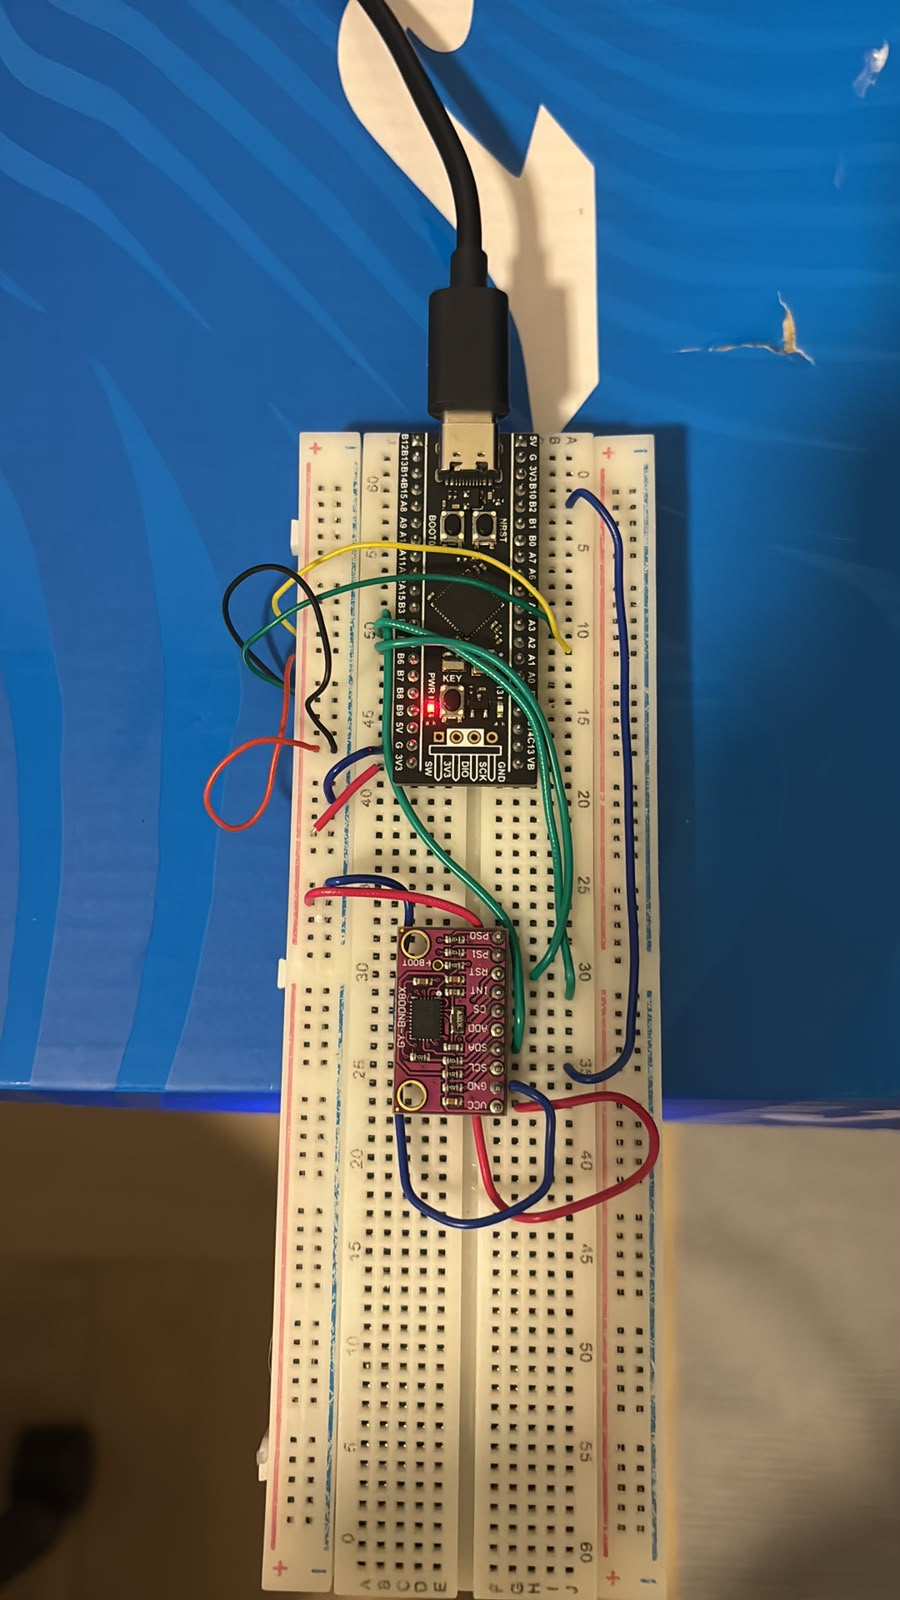
\includegraphics[width=0.4\textwidth]{images/testes/bno-bancada.png}
    \par\vspace{0.2cm}
    \footnotesize Fonte: elaborado pelos autores (2026).
\end{figure}

\begin{figure}[H]
    \centering
    \caption{Leituras estáticas e distribuição de ruído dos canais da IMU BNO08X.}
    \label{fig:ruido_bno08x}
    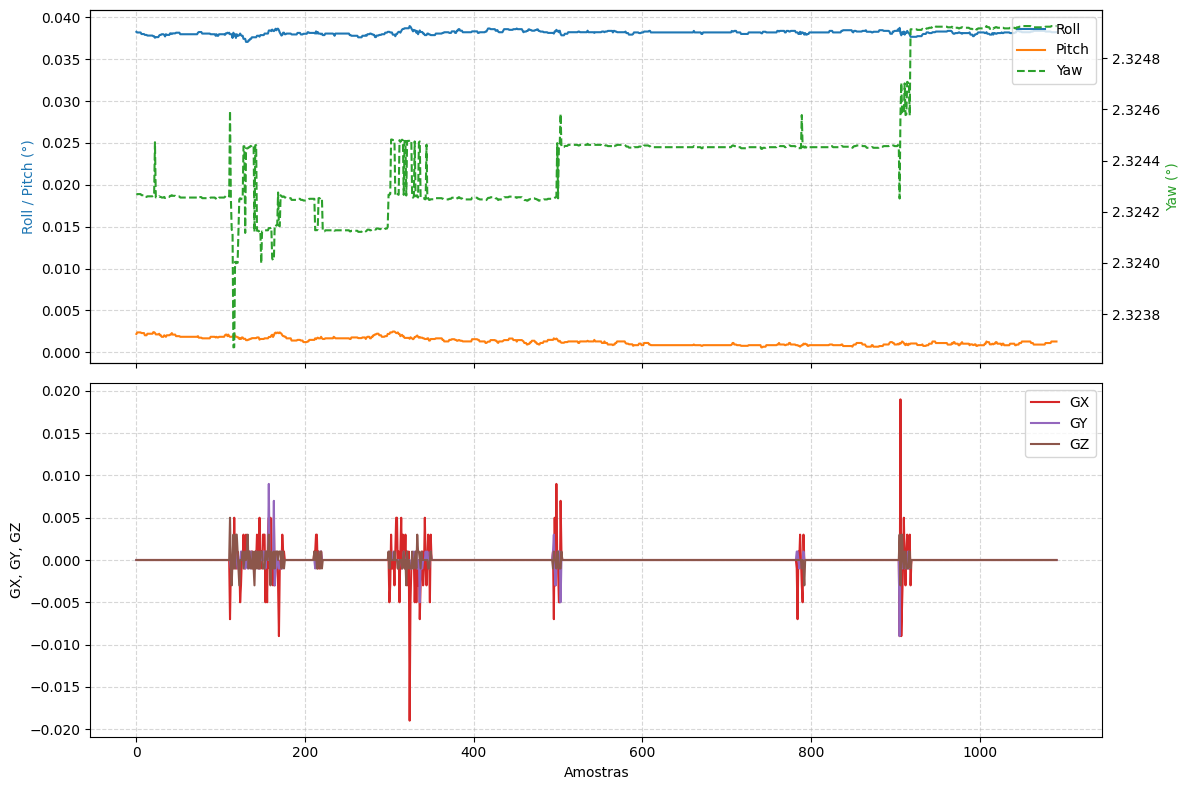
\includegraphics[width=0.85\textwidth]{images/resultados/plotBNO.png}
    \par\vspace{0.2cm}
    \footnotesize Fonte: elaborado pelos autores (2026).
\end{figure}

Com esses dados observados na Figura~\ref{fig:ruido_bno08x}, foi realizada a distribuição estatística do ruído observada em torno do valor médio (ajuste gaussiano).

\begin{figure}[H]
    \centering
    \caption{Distribuição de ruído em roll.}
    \label{fig:dn_roll}
    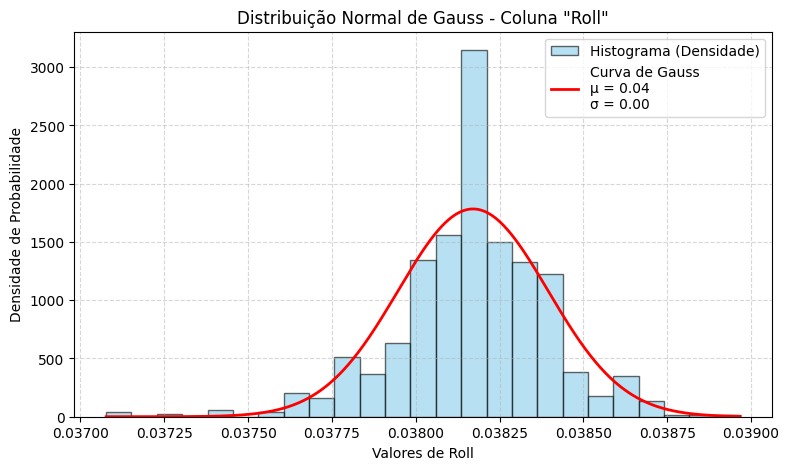
\includegraphics[width=0.85\textwidth]{images/resultados/DNRoll.png}
    \par\vspace{0.2cm}
    \footnotesize Fonte: elaborado pelos autores (2026).
\end{figure}

Observa-se na Figura~\ref{fig:dn_roll} que o sinal apresenta um comportamento compatível com a hipótese de ruído branco gaussiano adotada na formulação do Filtro de Kalman, com desvios contidos em uma faixa estreita em torno da média. Quanto ao determinismo temporal, os carimbos de tempo do \textit{log} mostram que a tarefa de registro no STM32F411 sob FreeRTOS manteve intervalo médio de 100,5~ms (9,95~Hz), com \textit{jitter} (desvio padrão de $\Delta t_i$) de 1,2~ms, intervalos entre 99 e 108~ms e nenhuma lacuna ao longo de aproximadamente 110~s de ensaio. Como o registro foi feito a 10~Hz, uma fração da taxa de 100~Hz dos \textit{reports} SH-2, esses valores descrevem a tarefa de \textit{log}; a taxa efetiva e o \textit{jitter} de cada \textit{report} exigem o registro individual com carimbo de tempo, previsto como etapa seguinte.
Os ensaios foram realizados com os motores desligados. A caracterização da influência da vibração dos motores sobre o ruído da IMU requer um ensaio com os motores em funcionamento, fora do escopo deste ensaio estático.

\subsection{Caracterização do sensor de fluxo óptico e LiDAR MTF-01}\label{subsec:res_mtf01}

De maneira análoga, o módulo MicoAir MTF-01 foi submetido a ensaios estáticos a uma distância vertical fixa de referência em relação ao solo, coletando $N = 729$ amostras consecutivas e operando via interface UART a 115200~bit/s com taxa nominal de saída de aproximadamente 100~Hz, sendo as leituras registradas a 10~Hz pelo \textit{log} USB. O contador de quadros recebidos avançou em média 10,04 quadros por intervalo de registro de 100~ms, o que corresponde a uma taxa efetiva de cerca de 100~Hz, sem erros de CRC, lacunas de sequência, erros de UART ou bytes descartados. A Figura~\ref{fig:bancada_mtf01} mostra o sensor fixado em um suporte provisório durante esse ensaio.

\begin{figure}[H]
    \centering
    \caption{Montagem provisória do sensor MTF-01 para o ensaio de bancada.}
    \label{fig:bancada_mtf01}
    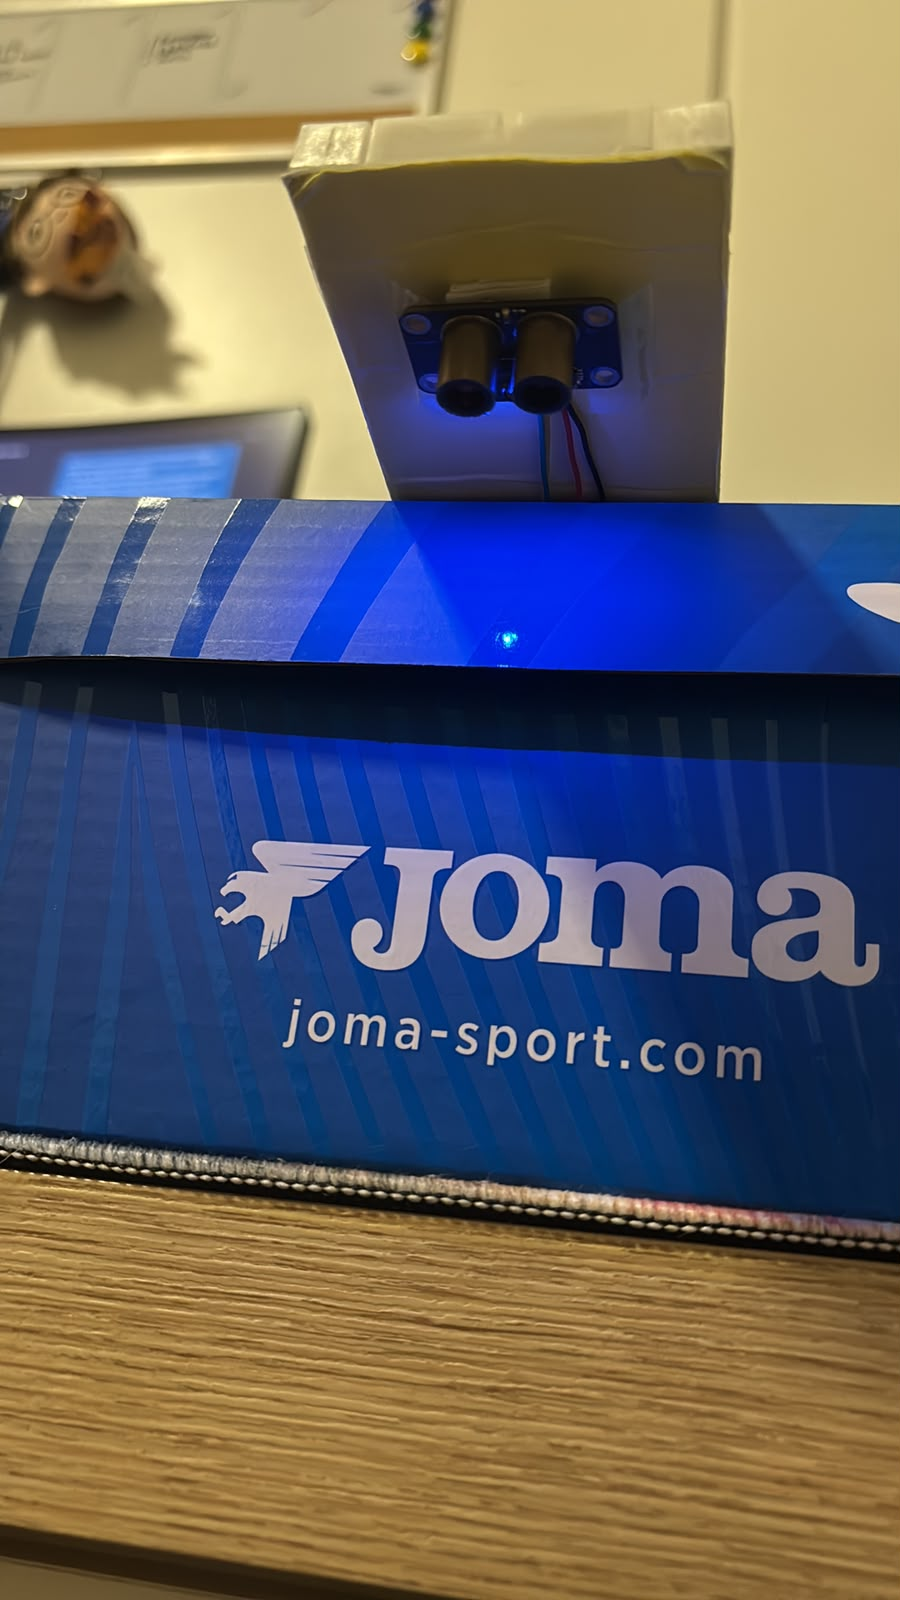
\includegraphics[width=0.4\textwidth]{images/testes/mtf01-bancada.png}
    \par\vspace{0.2cm}
    \footnotesize Fonte: elaborado pelos autores (2026).
\end{figure}

A Figura~\ref{fig:ruido_mtf01} ilustra as séries temporais obtidas para a medição de distância do sensor ToF ($z$) e para as componentes de velocidade linear horizontal ($\dot{x}$ e $\dot{y}$) derivadas do fluxo óptico.

\begin{figure}[H]
    \centering
    \caption{Caracterização experimental de ruído das medições do sensor MTF-01.}
    \label{fig:ruido_mtf01}
    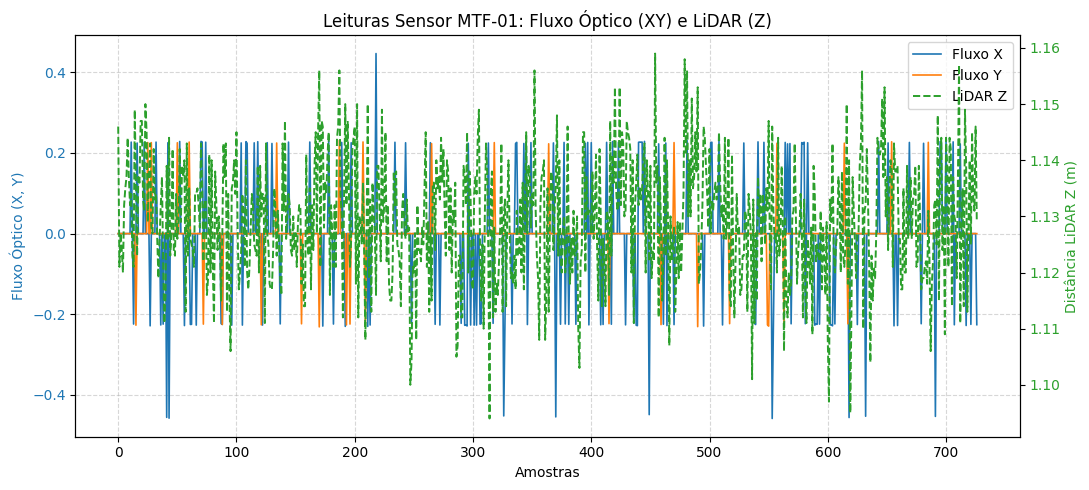
\includegraphics[width=0.85\textwidth]{images/resultados/plotMTF01.png}
    \par\vspace{0.2cm}
    \footnotesize Fonte: elaborado pelos autores (2026).
\end{figure}

Analisando a distribuição de ruído das medições do MTF-01 (Figura~\ref{fig:dn_xyz}), verificou-se que o comportamento estatístico das variáveis $z$, $\dot{x}$ e $\dot{y}$ também se aproxima de uma distribuição gaussiana, com desvios padrão relativamente baixos, indicando boa estabilidade e confiabilidade do sensor em condições estáticas.

\begin{figure}[H]
    \centering
    \caption{Distribuição de ruído em $z$, $\dot{x}$ e $\dot{y}$.}
    \label{fig:dn_xyz}
    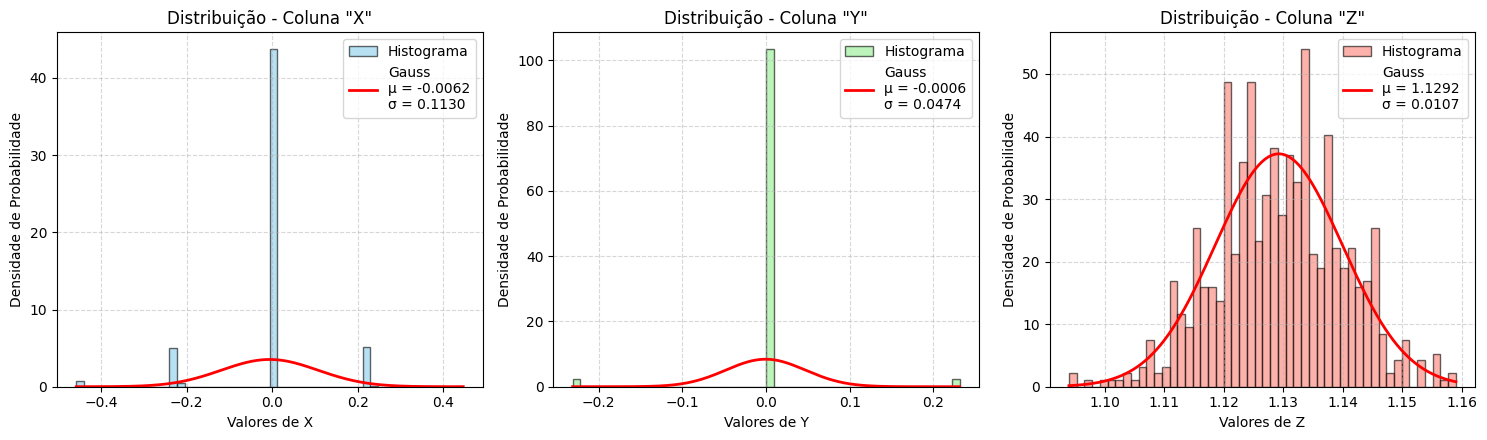
\includegraphics[width=0.85\textwidth]{images/resultados/DNXYZ.png}
    \par\vspace{0.2cm}
    \footnotesize Fonte: elaborado pelos autores (2026).
\end{figure}

O Quadro~\ref{qua:estatistica_sensores} consolida os parâmetros estatísticos extraídos dos ensaios de bancada para ambos os sensores, discriminando a média amostral (\textit{bias} residual), o desvio padrão ($\sigma_v$) e a variância resultante ($\sigma_v^2$) adotada na construção da diagonal da matriz $\mathbf{R}_v$.


\begin{quadro}[H]
\centering
\caption{Parâmetros estatísticos medidos nos sensores e variâncias aplicadas à matriz $\mathbf{R}_v$.}
\label{qua:estatistica_sensores}
\small
\renewcommand{\arraystretch}{1.25}
\setlength{\tabcolsep}{5pt} % Reduz suavemente o espaçamento horizontal entre as colunas
\begin{tabular}{|l|c|c|c|c|c|}
\hline
\textbf{Variável Medida} & \textbf{Sensor} & \textbf{Unidade} & \textbf{\shortstack{Média\\(\textit{Bias})}} & \textbf{\shortstack{Desvio Padrão\\($\sigma_v$)}} & \textbf{\shortstack{Variância\\($\sigma_v^2$)}} \\
\hline
Altitude ($z$) & MTF-01 & m & 1{,}1300 & $1{,}07 \times 10^{-2}$ & $1{,}15 \times 10^{-4}$ \\
Velocidade em $x$ ($\dot{x}$) & MTF-01 & m/s & 0{,}0000 & $1{,}13 \times 10^{-1}$ & $1{,}28 \times 10^{-2}$ \\
Velocidade em $y$ ($\dot{y}$) & MTF-01 & m/s & 0{,}0000 & $4{,}74 \times 10^{-2}$ & $2{,}20 \times 10^{-3}$ \\
Rolamento ($\phi$) & BNO08X & rad & 0{,}0382 & $2{,}24 \times 10^{-4}$ & $5{,}00 \times 10^{-8}$ \\
Arfagem ($\theta$) & BNO08X & rad & 0{,}0013 & $4{,}40 \times 10^{-4}$ & $1{,}94 \times 10^{-7}$ \\
Guinada ($\psi$) & BNO08X & rad & 2{,}3245 & $2{,}46 \times 10^{-4}$ & $6{,}04 \times 10^{-8}$ \\
Taxa de rolamento ($p$) & BNO08X & rad/s & 0{,}0000 & $1{,}44 \times 10^{-3}$ & $2{,}06 \times 10^{-6}$ \\
Taxa de arfagem ($q$) & BNO08X & rad/s & 0{,}0000 & $5{,}70 \times 10^{-4}$ & $3{,}24 \times 10^{-7}$ \\
Taxa de guinada ($r$) & BNO08X & rad/s & 0{,}0000 & $4{,}88 \times 10^{-4}$ & $2{,}38 \times 10^{-7}$ \\
\hline
\end{tabular}
\par\vspace{0.2cm}
\footnotesize Fonte: elaborado pelos autores (2026).
\end{quadro}

% =============================================================
\section{SIMULAÇÕES EM AMBIENTE MATLAB/SIMULINK}\label{sec:res_simulacoes}

Para realizar a validação do projeto de controle LQG antes dos ensaios de voo livre, foram conduzidas simulações numéricas no ambiente MATLAB/Simulink (versão R2024a). Primeiramente, implementou-se o modelo linearizado do quadricóptero em torno da condição de \textit{hover}, fundamentado nas matrizes de espaço de estados derivadas na Seção~\ref{subsubsec:linearizacao_sistema}, com a finalidade de verificar as propriedades estruturais de controlabilidade, observabilidade e estabilidade em malha fechada, além de sintonizar as matrizes de ponderação $\mathbf{Q}$ e $\mathbf{R}_{\mathrm{lqr}}$. Na sequência, o mesmo compensador LQG e os mesmos ganhos ($\mathbf{K}$ e $\mathbf{L}$) foram aplicados ao modelo dinâmico completo não linear do quadricóptero, incorporando os acoplamentos inerciais, as não linearidades trigonométricas e o ruído estocástico parametrizado pelo Quadro~\ref{qua:estatistica_sensores}.

\subsection{Verificação estrutural e sintonia das matrizes do controlador}\label{subsec:res_sintonia}

A verificação algébrica preliminar do par $(\mathbf{A}, \mathbf{B})$ confirmou o posto completo da matriz de controlabilidade ($\operatorname{rank}(\mathcal{C}) = 12$). Por outro lado, o par $(\mathbf{A}, \mathbf{C})$ apresentou deficiência de posto na matriz de observabilidade ($\operatorname{rank}(\mathcal{O}) = 10$), indicando que o sistema é completamente controlável nos 12 estados, porém não é observável nas posições translacionais $x$ e $y$ devido à ausência de medições de posição absoluta no plano horizontal. Dessa forma, comprova-se a necessidade da aplicação de um estimador de estados ótimo, como o Filtro de Kalman, para realizar a fusão sensorial, atenuar ruídos de medição e reconstruir dinamicamente o subsistema observável.

Após o processo iterativo de ajuste baseado no compromisso entre velocidade de resposta e limitação de esforço nos atuadores, definiram-se os seguintes valores para as diagonais das matrizes de ponderação de estados ($\mathbf{Q}$) e de controle ($\mathbf{R}_{\mathrm{lqr}}$):

\begin{equation}\label{eq:valores_Q_R_sim}
\begin{aligned}
\mathbf{Q} &= \operatorname{diag}\left(5,\, 5,\, 500,\, 500,\, 500,\, 50,\, 5,\, 5,\, 5,\, 10,\, 10,\, 5\right), \\
\mathbf{R}_{\mathrm{lqr}} &= \operatorname{diag}\left(0{,}1,\, 0{,}1,\, 0{,}1,\, 0{,}1\right).
\end{aligned}
\end{equation}

Todos os autovalores das matrizes de malha fechada do regulador ($\mathbf{A} - \mathbf{B}\mathbf{K}$) e do observador ($\mathbf{A} - \mathbf{L}\mathbf{C}$) posicionaram-se estritamente no semiplano esquerdo do plano complexo (ou no interior do círculo unitário, na formulação discreta com período de amostragem $T_s = 100$~ms), confirmando a estabilidade assintótica local do sistema.

\subsection{Desempenho do Filtro de Kalman na estimação de estados}\label{subsec:res_kalman}

A eficácia do Filtro de Kalman na rejeição do ruído de medição foi avaliada comparando-se os estados reais da planta, os sinais corrompidos pelo ruído sensorial ($\mathbf{y}$) e os estados reconstruídos pelo estimador ($\hat{\mathbf{x}}$). A Figura~\ref{fig:simulacao_kalman} apresenta a sobreposição entre a leitura ruidosa e a estimativa filtrada para as variáveis do sistema.

\begin{figure}[H]
    \centering
    \caption{Comparação entre estados reais, medições ruidosas e estimativas do Filtro de Kalman.}
    \label{fig:simulacao_kalman}
    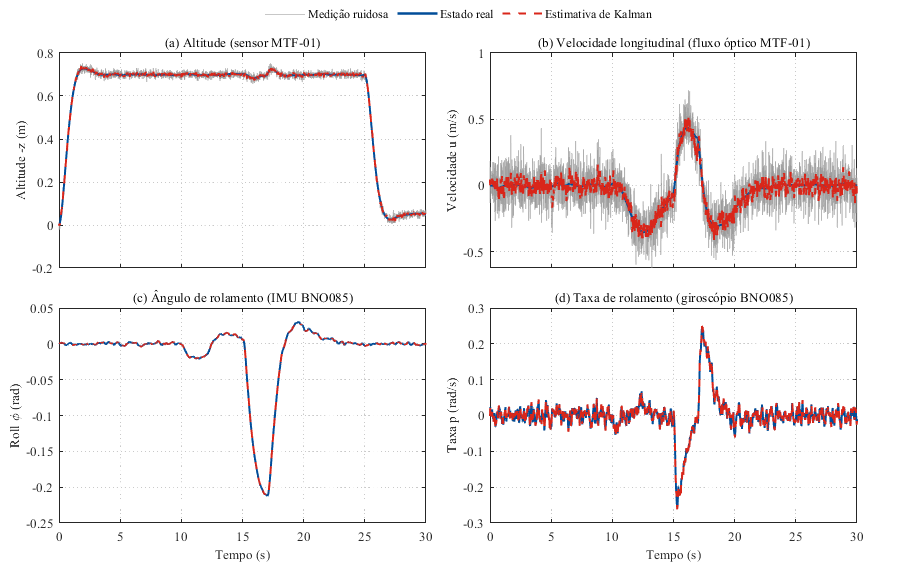
\includegraphics[width=0.85\textwidth]{images/resultados/kalman.png}
    \par\vspace{0.2cm}
    \footnotesize Fonte: elaborado pelos autores (2026).
\end{figure}

Verifica-se na Figura~\ref{fig:simulacao_kalman} que o estimador atenua significativamente as flutuações de alta frequência oriundas dos sensores sem introduzir atraso de fase excessivo na malha, fornecendo uma estimativa suave ($\hat{\mathbf{x}}$) para o cálculo da lei de controle LQR e evitando que o ruído de medição seja amplificado pelos ganhos da matriz $\mathbf{K}$ nos comandos enviados aos motores.

\subsection{Comparação entre o modelo linear e o modelo não linear}\label{subsec:res_linear_vs_naolinear}

Para avaliar o domínio de validade da linearização por série de Taylor e a robustez do controlador LQG frente às dinâmicas não lineares do quadricóptero, ambos os modelos foram submetidos às mesmas condições iniciais e perfis de referência. O ensaio consiste em inicializar a aeronave na origem do referencial inercial, $[x,\, y,\, z]^{\top} = [0,\, 0,\, 0]^{\top}\text{ m}$, comandando-se inicialmente uma manobra de subida para a altitude de $0{,}7\text{ m}$. Em seguida, aplica-se uma rotação de $45^\circ$ ($\pi/4\text{ rad}$) em torno do eixo de guinada ($\psi$) em $t = 5\text{ s}$ e, posteriormente, um deslocamento translacional no plano horizontal em $t = 10\text{ s}$ (suavizado por um limitador de taxa) até as coordenadas de magnitude $[1{,}0,\, 1{,}0]\text{ m}$. Após a estabilização, o sistema é submetido, entre $t = 15\text{ s}$ e $t = 17\text{ s}$, a um distúrbio externo de atitude equivalente a $10^\circ$ em rolamento ($\phi$), $-5^\circ$ em arfagem ($\theta$) e $10^\circ$ em guinada ($\psi$), devendo rejeitar a perturbação e retomar a atitude de equilíbrio. Por fim, em $t = 25\text{ s}$, executa-se a manobra de redução de altitude (pouso).

A Figura~\ref{fig:comp_atitude} apresenta a resposta transitória comparativa dos ângulos de atitude ($\phi$, $\theta$ e $\psi$) entre o modelo linear e o modelo não linear, a Figura~\ref{fig:comp_posicaoXY} exibe o rastreamento de posição $x$ e $y$, e por fim a Figura~\ref{fig:comp_posicaoZ} mostra o rastreamento de posição $z$.

\begin{figure}[H]
    \centering
    \caption{Comparação da resposta de atitude ($\phi, \theta, \psi$): modelo linear vs. modelo não linear.}
    \label{fig:comp_atitude}
    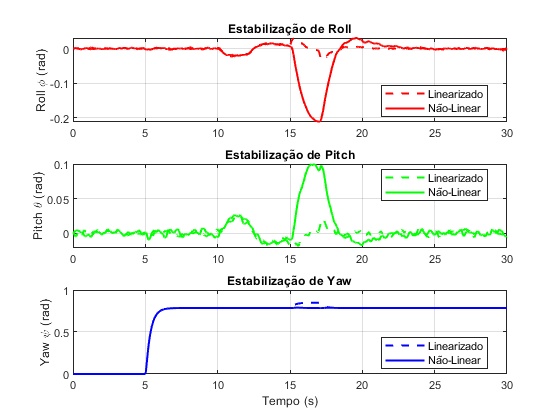
\includegraphics[width=0.85\textwidth]{images/resultados/comparacao_atitude.png}
    \par\vspace{0.2cm}
    \footnotesize Fonte: elaborado pelos autores (2026).
\end{figure}

\begin{figure}[H]
    \centering
    \caption{Comparação da resposta de posição ($x, y, z$): modelo linear vs. modelo não linear.}
    \label{fig:comp_posicaoXY}
    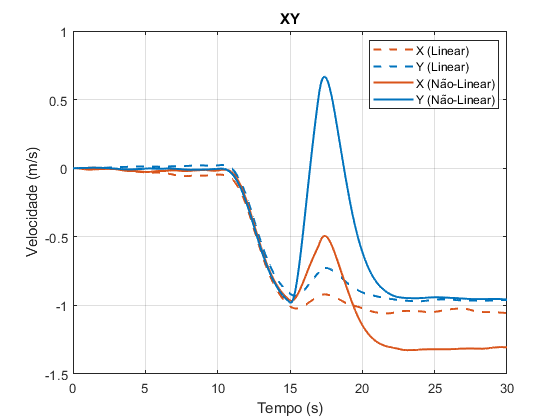
\includegraphics[width=0.85\textwidth]{images/resultados/comparacao_posicaoXY.png}
    \par\vspace{0.2cm}
    \footnotesize Fonte: elaborado pelos autores (2026).
\end{figure}

\begin{figure}[H]
    \centering
    \caption{Comparação da resposta de posição ($x, y, z$): modelo linear vs. modelo não linear.}
    \label{fig:comp_posicaoZ}
    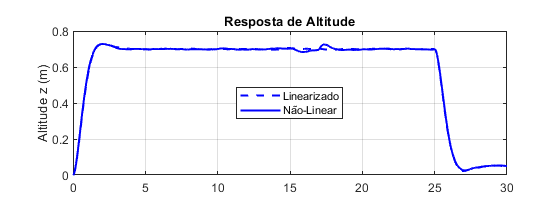
\includegraphics[width=0.85\textwidth]{images/resultados/comparacao_posicaoZ.png}
    \par\vspace{0.2cm}
    \footnotesize Fonte: elaborado pelos autores (2026).
\end{figure}

Adicionalmente, a Figura~\ref{fig:esforco_motores} ilustra o comportamento das velocidades angulares comandadas aos quatro rotores ($\omega_1, \omega_2, \omega_3, \omega_4$) durante a manobra, demonstrando que as ações de controle convergem para a rotação nominal de equilíbrio ($\omega_0 \approx 146{,}23$~rad/s) e permanecem dentro dos limites físicos de saturação dos propulsores.

\begin{figure}[H]
    \centering
    \caption{Velocidades angulares comandadas aos quatro motores ($\omega_1$ a $\omega_4$) na simulação.}
    \label{fig:esforco_motores}
    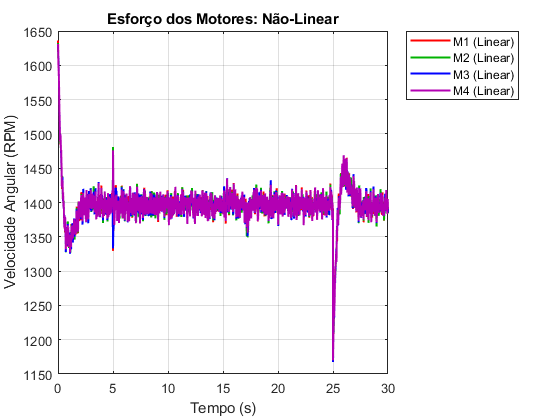
\includegraphics[width=0.85\textwidth]{images/resultados/esforco_motores.png}
    \par\vspace{0.2cm}
    \footnotesize Fonte: elaborado pelos autores (2026).
\end{figure}

Para quantificar objetivamente a aderência entre a aproximação linear e a planta não linear, conforme definido na Seção~\ref{subsec:metricas_lqr}, o Quadro~\ref{qua:metricas_simulacao} resume os indicadores de desempenho obtidos para cada grau de liberdade: Raiz do Erro Quadrático Médio (RMSE), Erro Absoluto Médio (MAE), sobressinal percentual ($M_p$), tempo de acomodação ($t_s$ para banda de 2\%) e erro em regime permanente ($e_{\mathrm{ss}}$).

\begin{quadro}[H]
\centering
\caption{Comparativo das métricas de desempenho de controle entre o modelo linear e o não linear.}
\label{qua:metricas_simulacao}
\small
\renewcommand{\arraystretch}{1.25}
\setlength{\tabcolsep}{5pt} % Reduz levemente o espaçamento horizontal entre as colunas
\begin{tabular}{|l|c|c|c|c|c|c|}
\hline
\textbf{Variável / Modelo} & \textbf{Unid.} & \textbf{RMSE} & \textbf{MAE} & \textbf{\shortstack{Sobressinal\\($M_p$)}} & \textbf{\shortstack{Acomodação\\($t_s$)}} & \textbf{\shortstack{Erro Estac.\\($e_{\mathrm{ss}}$)}} \\
\hline
\multicolumn{7}{|l|}{\textbf{Modelo Linearizado}} \\
\hline
Posição $x$ & m & 0,289 & 0,205 & 0,0\% & 14,90~s & 0,073 \\
Posição $y$ & m & 0,271 & 0,177 & 2,5\% & 14,90~s & 0,023 \\
Altitude $z$ & m & 0,098 & 0,022 & 4,2\% & 2,73~s & 0,002 \\
Rolamento ($\phi$) & graus & 0,633 & 0,447 & 1,7$^\circ$\textsuperscript{*} & 2,95~s & 0,009 \\
Arfagem ($\theta$) & graus & 0,543 & 0,410 & 1,6$^\circ$\textsuperscript{*} & 2,93~s & 0,282 \\
Guinada ($\psi$) & graus & 6,385 & 1,630 & 0,0\% & 1,27~s & 0,001 \\
\hline
\multicolumn{7}{|l|}{\textbf{Modelo Não Linear Completo}} \\
\hline
Posição $x$ & m & 0,363 & 0,313 & 29,4\% & 14,90~s & 0,285 \\
Posição $y$ & m & 0,725 & 0,544 & 0,0\% & 14,90~s & 0,132 \\
Altitude $z$ & m & 0,097 & 0,023 & 4,2\% & 17,69~s & 0,001 \\
Rolamento ($\phi$) & graus & 3,931 & 2,082 & 12,2$^\circ$\textsuperscript{*} & 6,41~s & 0,040 \\
Arfagem ($\theta$) & graus & 1,955 & 1,162 & 6,0$^\circ$\textsuperscript{*} & 5,63~s & 0,005 \\
Guinada ($\psi$) & graus & 6,387 & 1,632 & 0,0\% & 1,27~s & 0,003 \\
\hline
\end{tabular}
\par\vspace{0.15cm}
\footnotesize \textsuperscript{*}Para $\phi$ e $\theta$ (regulação em $0^\circ$), $M_p$ representa a deflexão angular máxima absoluta atingida nas manobras e rejeição de distúrbios.\\
Fonte: elaborado pelos autores (2026).
\end{quadro}

A análise comparativa das curvas e das métricas do Quadro~\ref{qua:metricas_simulacao} demonstra que, dentro do envelope operacional de pequenos ângulos ($|\phi|, |\theta| \le 15^\circ$), as respostas dos modelos linear e não linear apresentam elevada concordância. As pequenas divergências observadas durante os instantes iniciais do regime transitório no modelo não linear devem-se ao termo de acoplamento trigonométrico do empuxo ($\cos\phi\cos\theta$) na dinâmica vertical e aos termos giroscópicos cruzados nas equações rotacionais, os quais são prontamente compensados pela malha fechada LQG sem comprometer a estabilidade do sistema.

Graficamente se observa um grande desvio nas posições $x$ e $y$ do modelo não linear, no momento que ocorre o distúrbio. Após a tentativa de estabilização, acaba ocorrendo um erro de regime permanente, que é explicado pela falta de observabilidade das posições horizontais, uma vez que o sistema não possui sensores de posição absoluta. Por outro lado, a altitude $z$ e os ângulos de atitude ($\phi$, $\theta$, $\psi$) apresentam excelente rastreamento e rejeição de distúrbios, com erros em regime permanente desprezíveis.

\section{Validação em Voo Real}\label{sec:resultados_voo}

Após a calibração do Filtro de Kalman e a validação teórica das matrizes de ganho do controlador ótimo em ambiente de simulação, procedeu-se aos ensaios práticos de voo. O objetivo desta etapa consistiu em avaliar a capacidade do controlador LQR/LQG embarcado em manter o quadricóptero estabilizado na origem do plano horizontal ($X=0, Y=0$) e na altitude de referência de $15\,\mathrm{cm}$. Os dados telemétricos foram transmitidos via interface serial e gravados com uma taxa de amostragem de $50\,\mathrm{Hz}$.

A Figura \ref{fig:telemetria_atitude} apresenta a resposta temporal do sistema em malha fechada para as variáveis de atitude (rolamento, arfagem e guinada), a altitude em relação ao solo e o respectivo esforço de controle aplicado aos atuadores. A decolagem autônoma ocorreu aproximadamente no instante $t = 7\,\mathrm{s}$.

\begin{figure}[H]
\centering
\caption{Telemetria completa do voo: atitude, altitude e esforço de controle.}
\label{fig:telemetria_atitude}
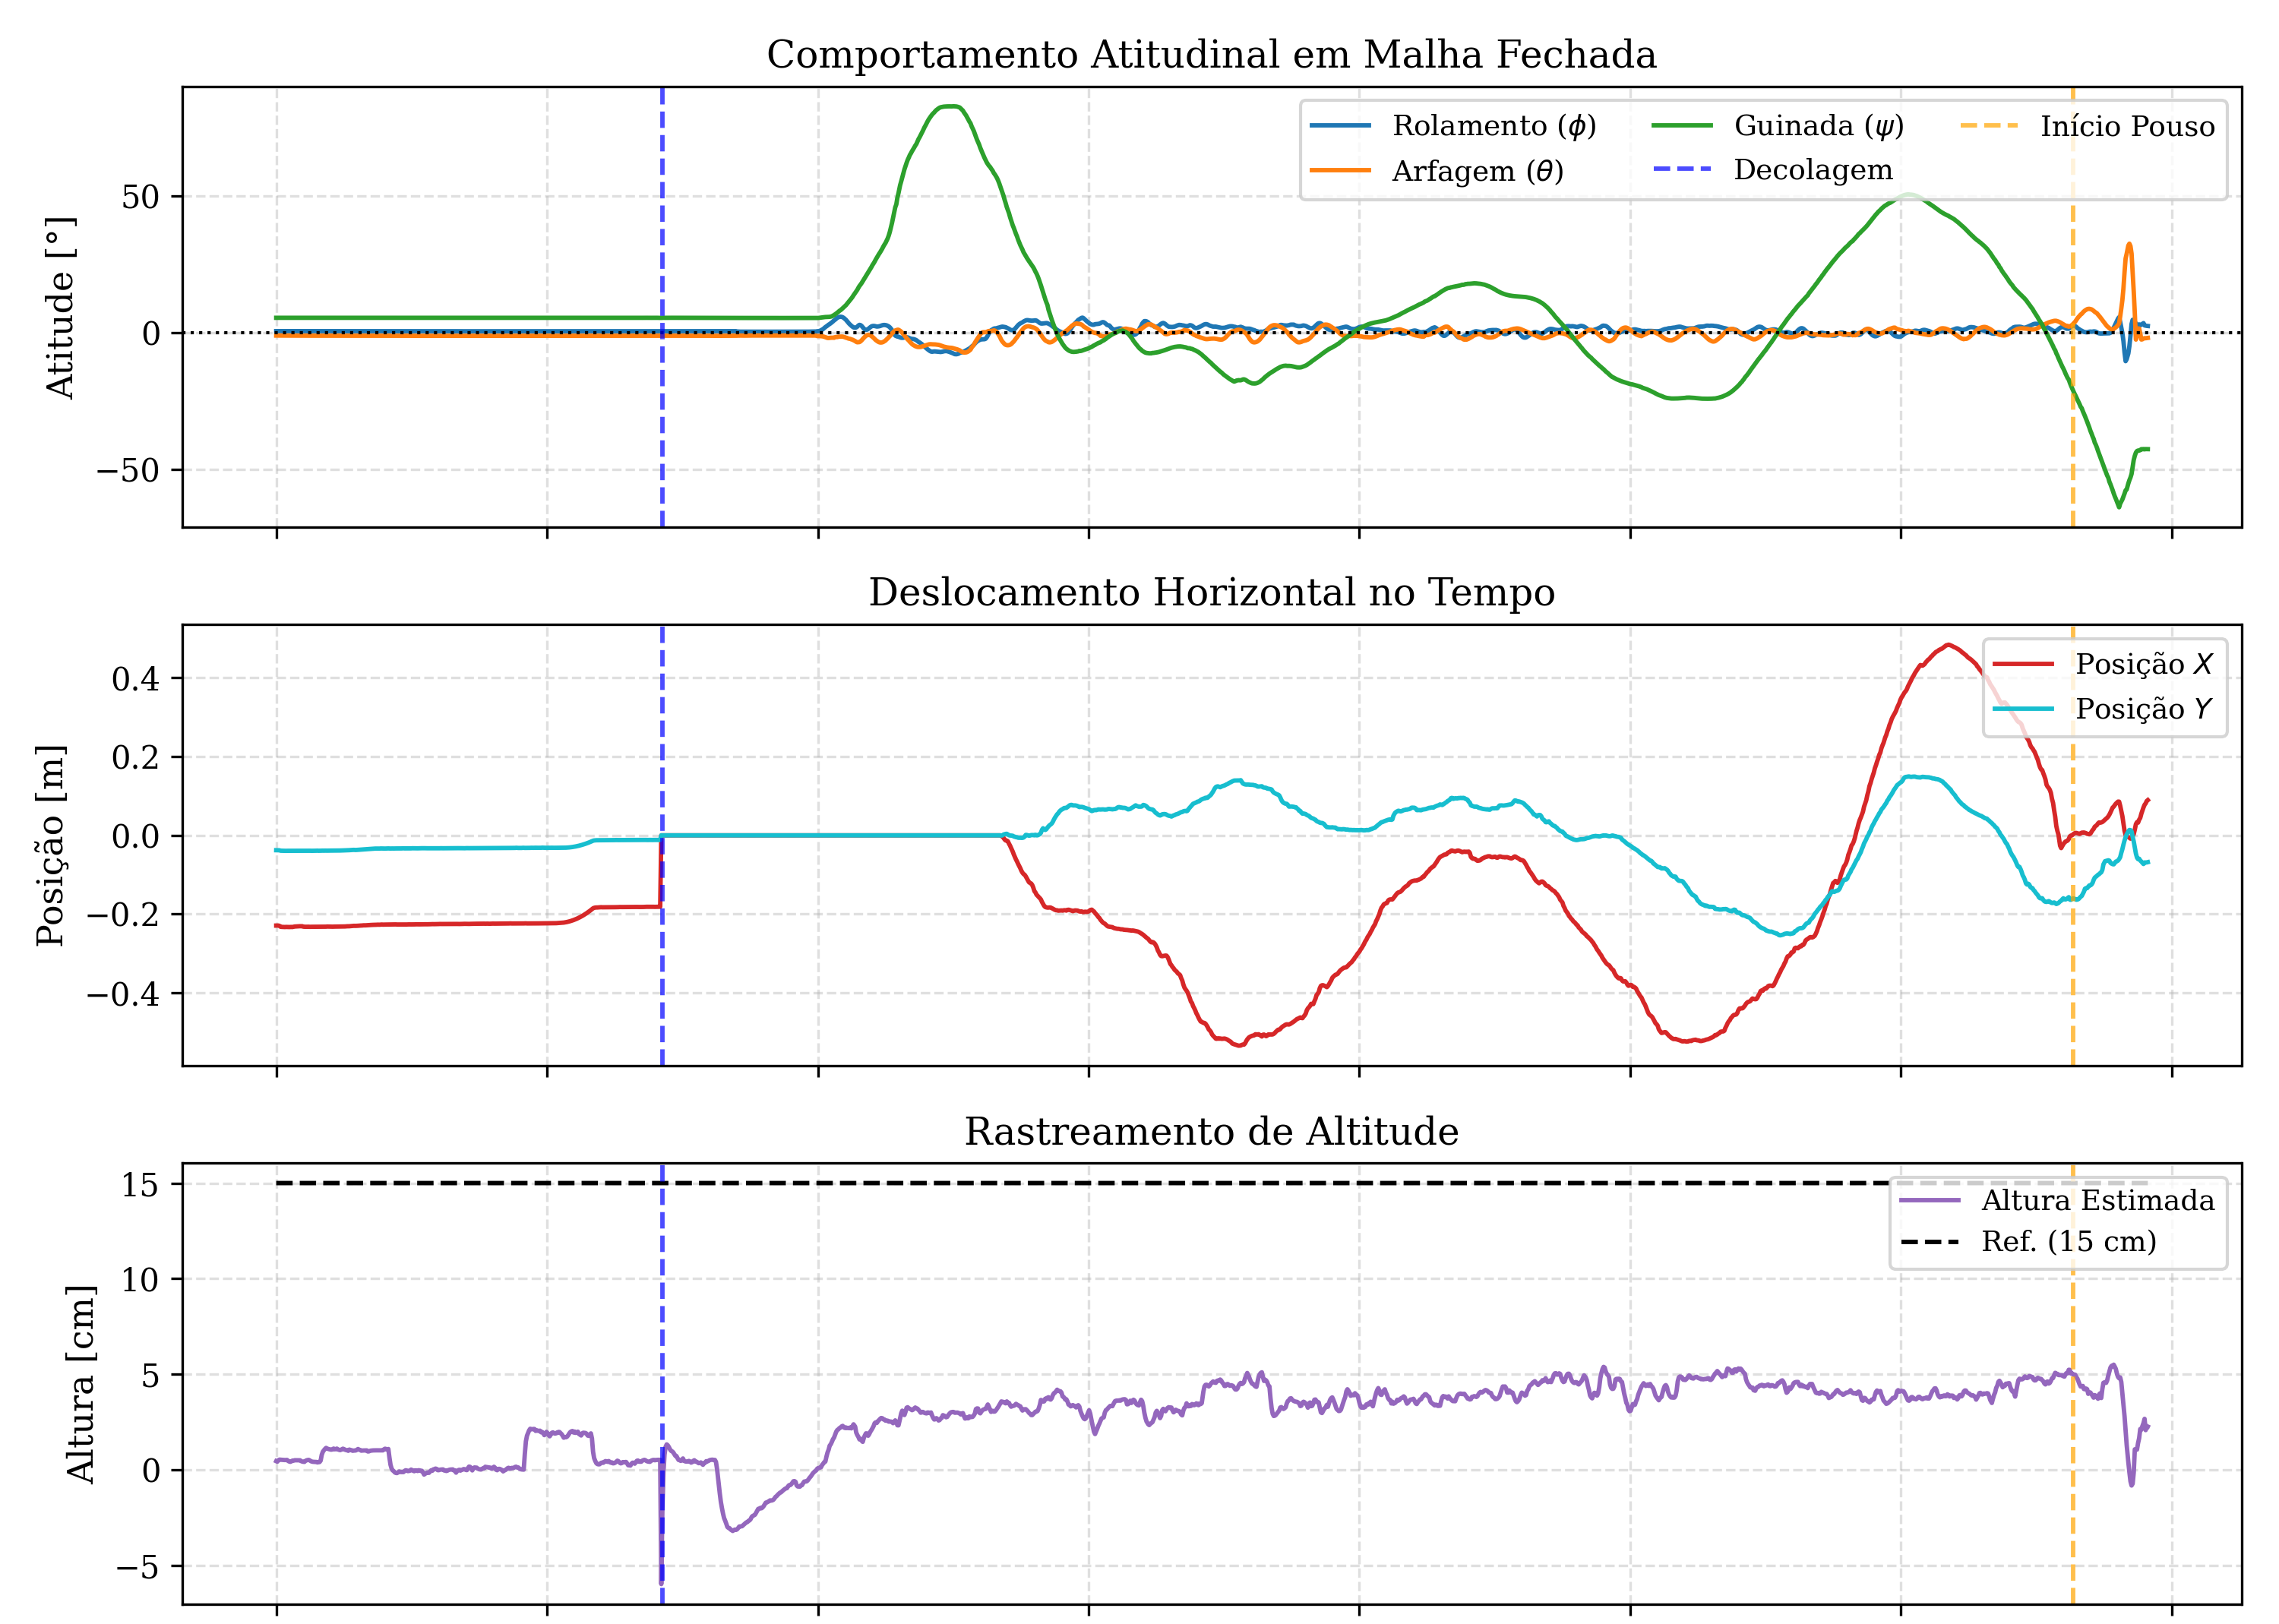
\includegraphics[width=0.9\textwidth]{images/resultados/telemetria_voo_completa.png}
\vspace{0.2cm}
\par\footnotesize Fonte: elaborado pelos autores (2026).
\end{figure}

A análise das curvas de atitude revela que o controlador foi capaz de manter os ângulos de rolamento ($\phi$) e arfagem ($\theta$) estabilizados em uma faixa estreita de oscilação em torno de suas referências, mesmo sob os ruídos mecânicos de alta frequência gerados pelos propulsores. A guinada ($\psi$), por outro lado, não foi regulada, variando entre aproximadamente $+80^\circ$ e $-60^\circ$ ao longo do voo. A altura estimada estabilizou-se entre 4 e 5~cm, abaixo da referência de 15~cm. Em ensaios complementares, com o deslocamento horizontal restringido por um apoio físico, a altura de referência foi alcançada, o que indica que a manutenção da posição horizontal na origem é a condição que falta para a subida até a altura de referência em voo livre.

Contudo, apesar da estabilidade de rolamento e arfagem, a malha de controle de posição externa não atingiu o desempenho projetado. A Figura \ref{fig:telemetria_xy} ilustra a trajetória estimada do quadricóptero no plano cartesiano, evidenciando uma oscilação não compensada em torno da origem, com excursões de até cerca de 0,5~m no eixo $X$. 

\begin{figure}[H]
\centering
\caption{Trajetória estimada do veículo no plano horizontal ($X \times Y$).}
\label{fig:telemetria_xy}
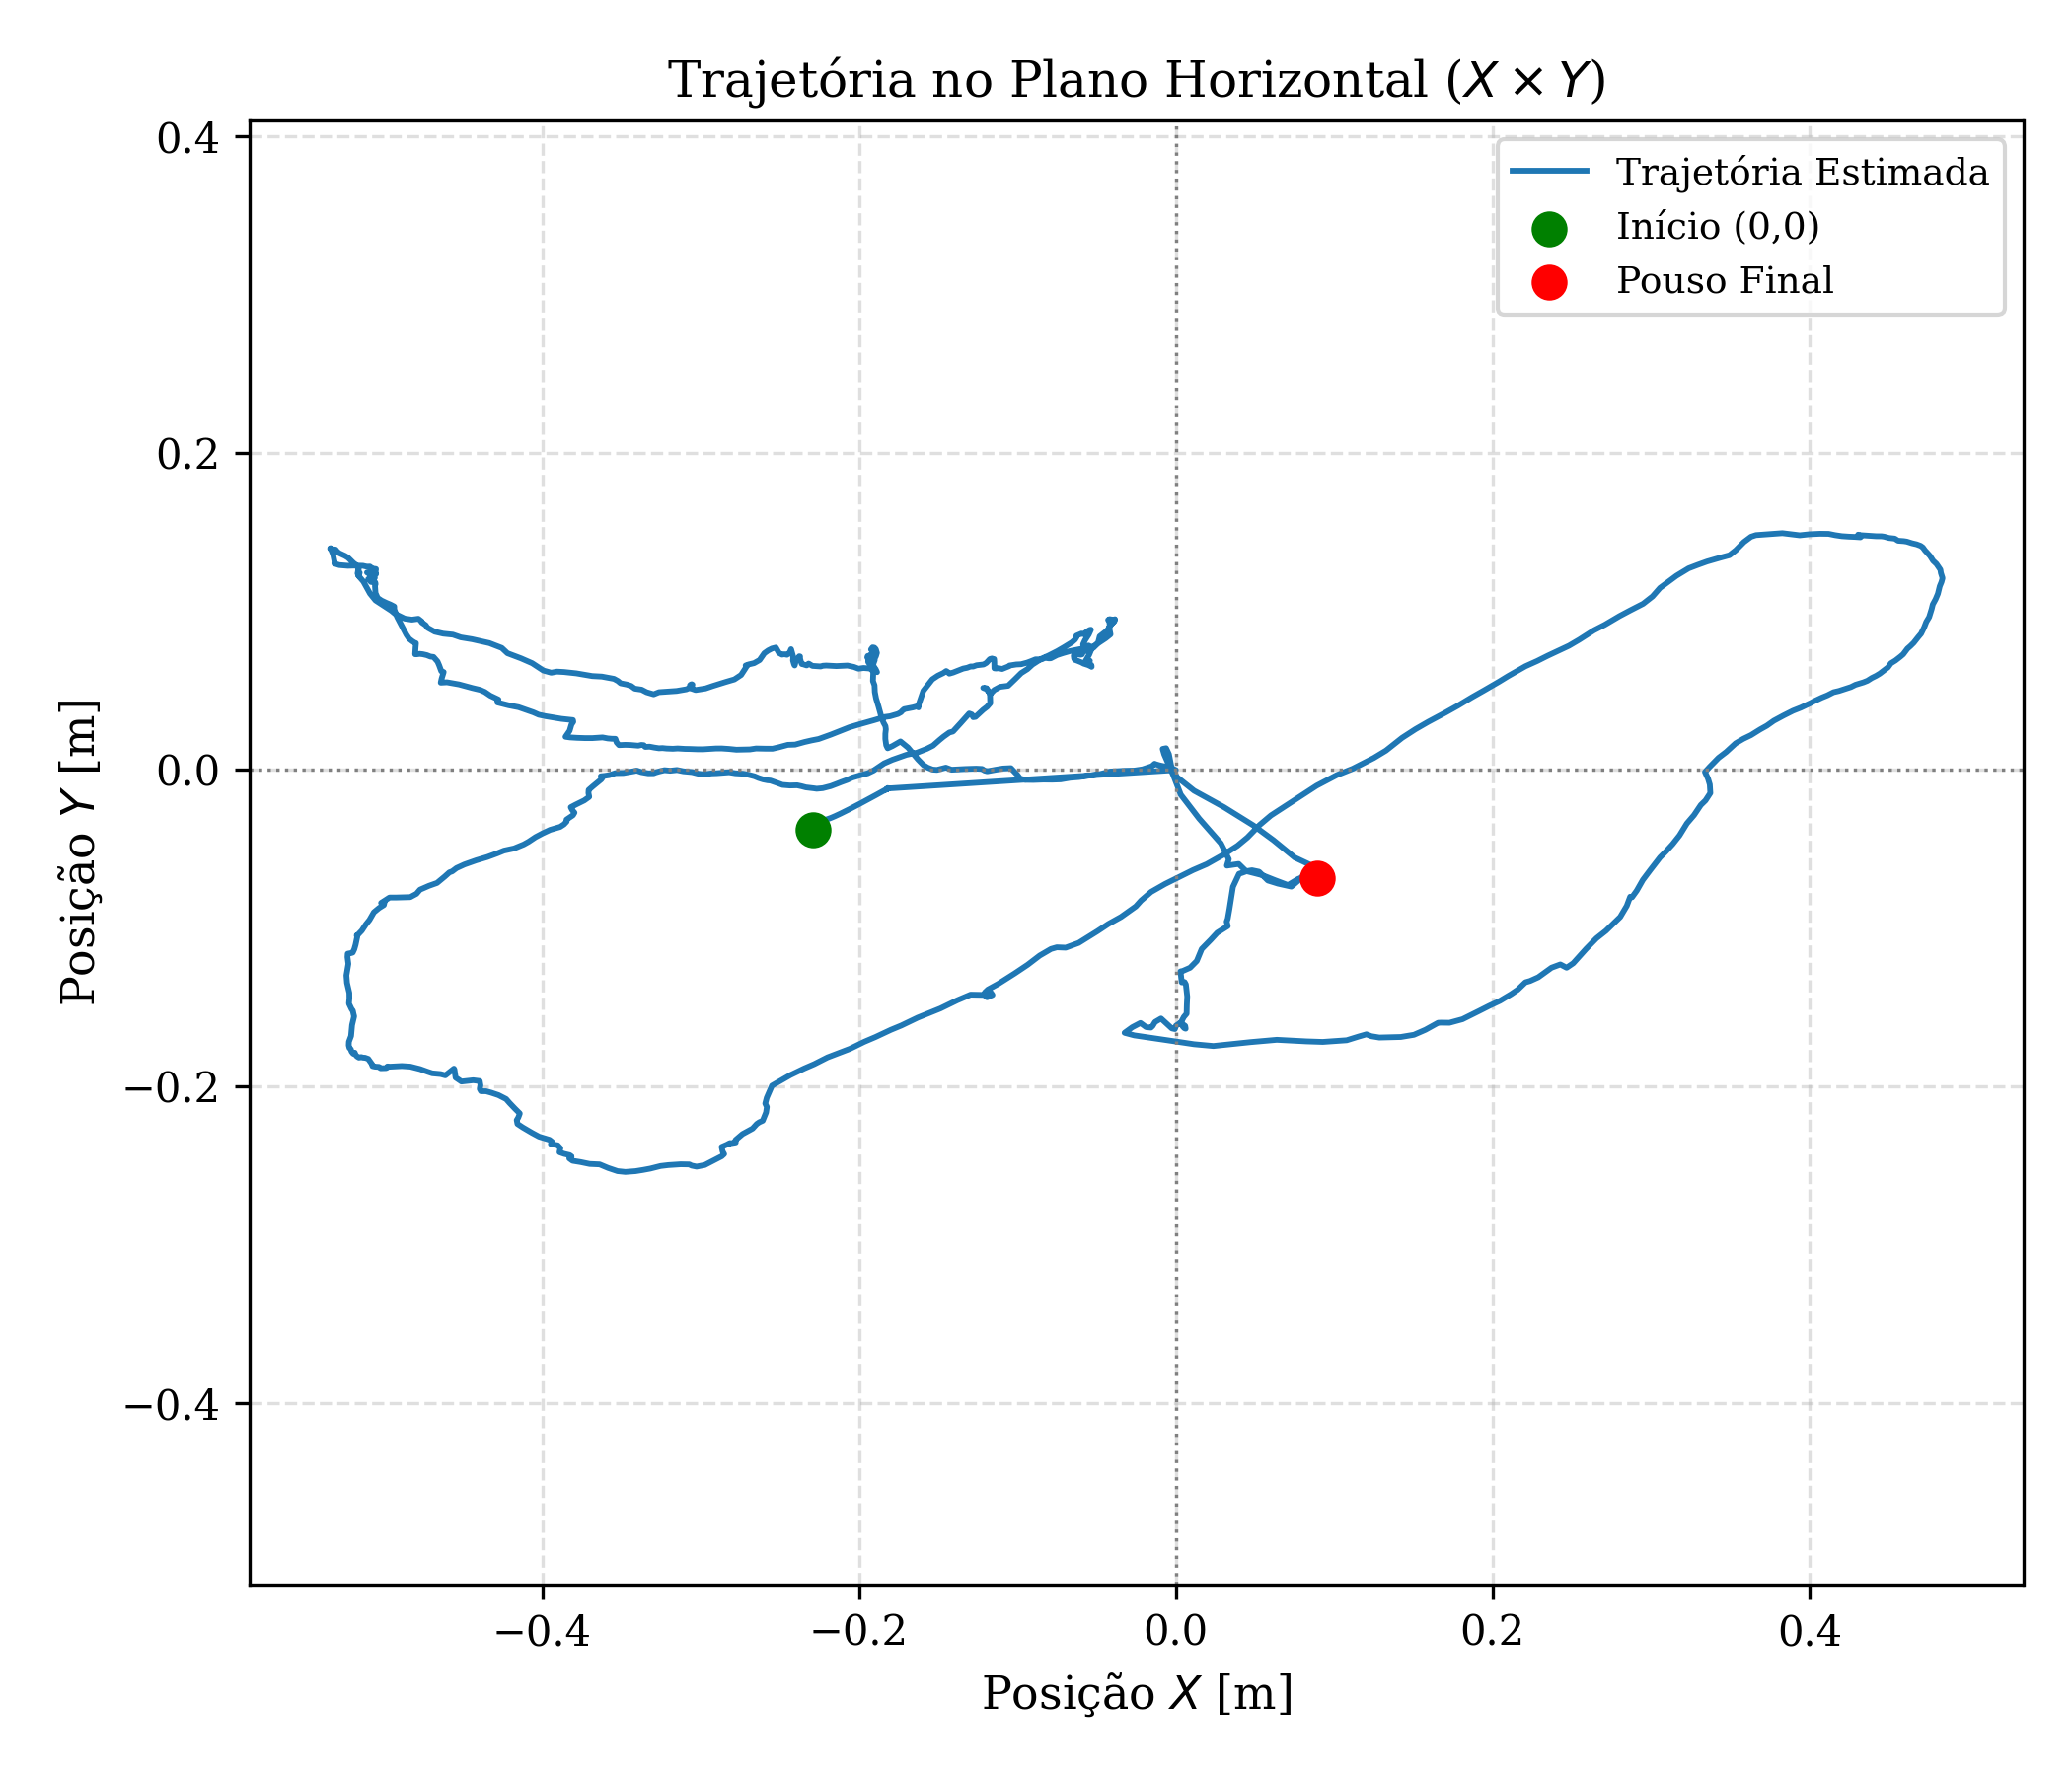
\includegraphics[width=0.7\textwidth]{images/resultados/trajetoria_plano_xy.png}
\vspace{0.2cm}
\par\footnotesize Fonte: elaborado pelos autores (2026).
\end{figure}

Observa-se que, durante a subida em direção à altura de referência, o veículo não manteve a posição horizontal na origem. Ao se deslocar, ficou sujeito a forças externas presentes no ambiente de ensaio, como o cabo USB conectado, a proximidade de paredes, o contato com as mãos do operador ou correntes de ar em espaço aberto, e foram essas forças que o levaram a ultrapassar a inclinação máxima de segurança estabelecida no firmware. Nesse limiar, a supervisão acionou a rotina de pouso seguida do corte dos motores (\textit{failsafe}). Nos ensaios em que nenhuma força externa atuou sobre o veículo, a inclinação de \textit{failsafe} não foi atingida.

A divergência na posição plana, coexistindo com rolamento e arfagem estabilizados, sugere a presença de perturbações externas constantes não modeladas (como um deslocamento do centro de massa em relação à controladora de voo ou correntes de ar) combinadas ao acúmulo de erros de integração (\textit{drift}) típicos do sensor de fluxo óptico MTF-01 ao operar perto do solo. Em trabalhos futuros, a introdução de uma malha adaptativa para estimar o desbalanceamento estático ou o refinamento empírico da matriz de covariância de ruído do processo ($Q$) poderiam mitigar esse comportamento.

\subsection{Registro do voo sem cabo e acompanhamento pelo terminal}
\label{subsec:voo_sem_cabo}

A imagem (a) da Figura~\ref{fig:voo_terminal} registra o protótipo em voo físico, sem cabo conectado ao computador. Esse registro difere dos ensaios de comunicação com o veículo simulado: neste caso, os motores estavam em funcionamento e o drone se deslocava no ambiente real.



O ensaio é iniciado pelo operador no terminal do Raspberry Pi, por meio do programa de teste de voo pairado. O comando \texttt{hover-test}, com a opção \texttt{--motors}, solicita a execução física do teste; as opções \texttt{--height} e \texttt{--time} definem a altura de referência e a duração solicitada. Também podem ser fornecidos parâmetros de controle e uma identificação para o registro. O Raspberry Pi coordena o ensaio e coleta a telemetria, enquanto o STM32 executa o controle do veículo. Ao final, o programa salva o registro no Raspberry Pi e apresenta um resumo no terminal. O encerramento pode ocorrer antes do previsto se uma condição de supervisão interromper o teste.

A imagem (b) da Figura~\ref{fig:voo_terminal} apresenta esse relatório ao final de um teste físico de decolagem. No registro mostrado, a referência era de 15~cm, mas a altura máxima informada foi de 6,3~cm. O programa indicou que o alvo não foi atingido em 26~s e iniciou o pouso, seguido do desarme. Foram registradas 2082 amostras de telemetria a 50~Hz, com 3,2\% de perdas informadas no relatório. Esses dados documentam o acompanhamento do ensaio e a limitação de altitude observada nesse registro; não demonstram que a referência de decolagem tenha sido alcançada.

\begin{figure}[htbp]
    \centering
    \caption{Registro conjunto do ensaio físico: (a) protótipo em voo sem cabo; (b) relatório apresentado no terminal ao término do teste.}
    \label{fig:voo_terminal}
    \begin{minipage}[t]{0.48\textwidth}
        \centering
        \vspace{0pt}
        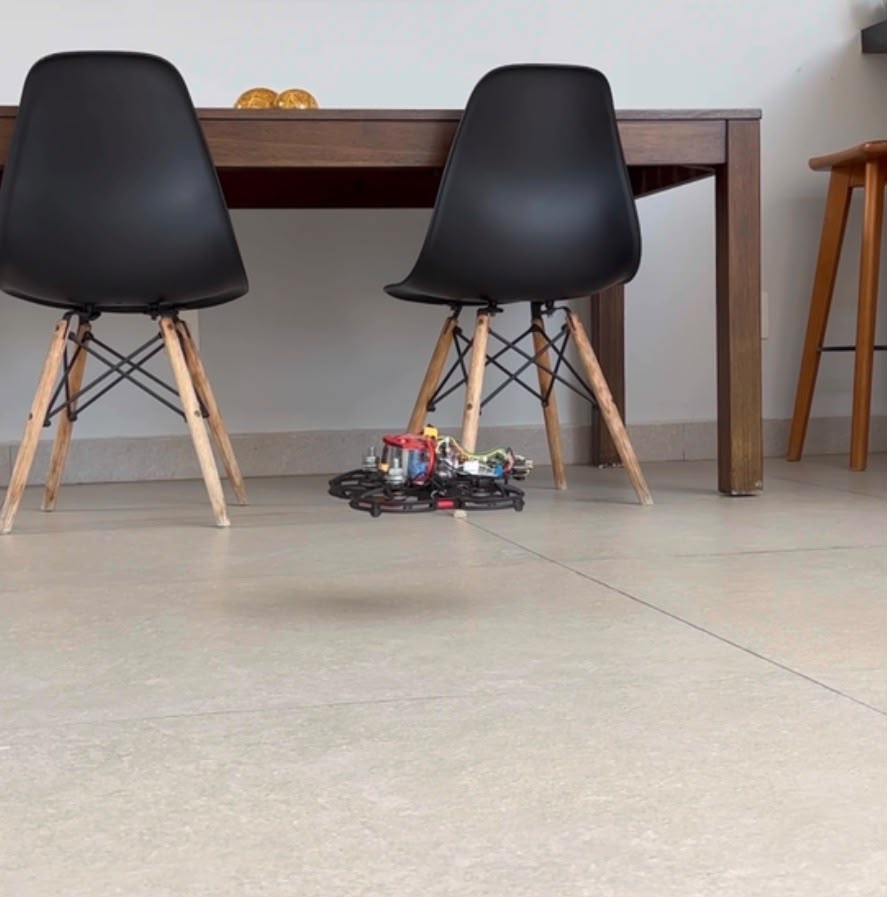
\includegraphics[width=\linewidth,height=8cm,keepaspectratio]{images/resultados/drone_sem_fio.jpeg}
        \par\smallskip{\footnotesize (a) Protótipo em voo.}
    \end{minipage}
    \hfill
    \begin{minipage}[t]{0.48\textwidth}
        \centering
        \vspace{0pt}
        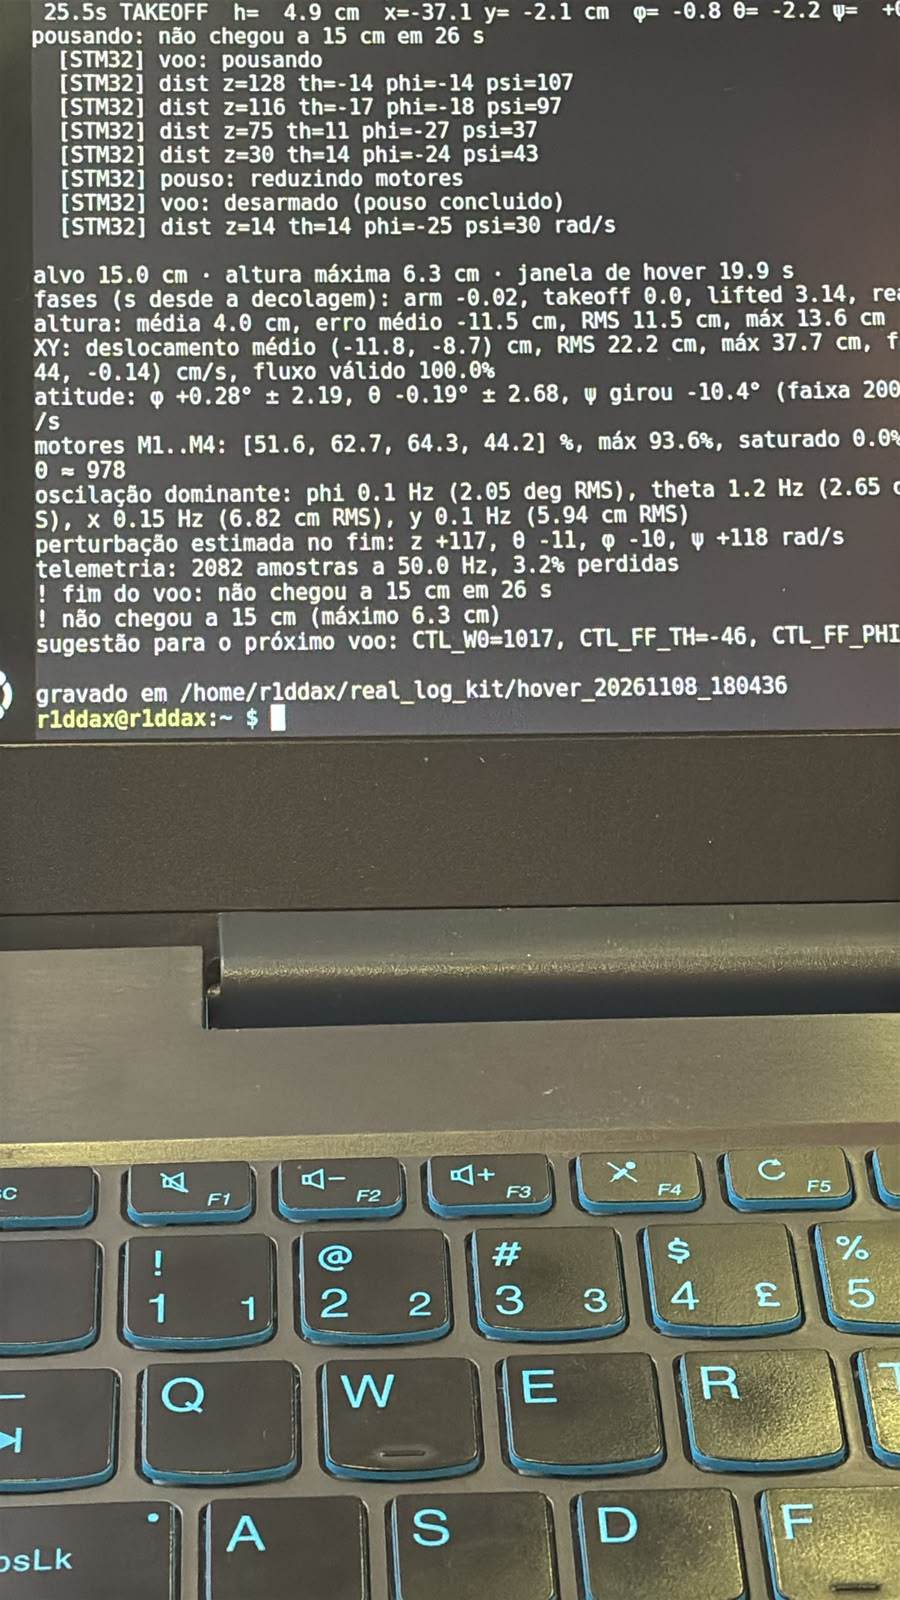
\includegraphics[width=\linewidth,height=8cm,keepaspectratio]{images/resultados/terminal.jpeg}
        \par\smallskip{\footnotesize (b) Relatório do ensaio.}
    \end{minipage}
    \par\vspace{0.2cm}
    \footnotesize Fonte: elaborado pelos autores (2026).
\end{figure}

% Comunicação Raspberry Pi <-> STM32 (testes, ensaios no STM32, problemas corrigidos)
% ============================================================================
% RESULTADOS — comunicação entre o Raspberry Pi e o STM32 (DroneLink)
% Chamado em partes/textuais/resultados.tex.
% Registro do ensaio: DroneSTM32/docs/resultados_comunicacao/
%   dronelink_20261107_225922.json (tools/pi/ensaios/ensaio_dronelink.py).
% ============================================================================

\section{COMUNICAÇÃO ENTRE O COMPUTADOR DE MISSÃO E O CONTROLADOR DE VOO}\label{sec:res_comunicacao}

Esta seção apresenta os resultados dos três níveis de ensaio descritos na Seção~\ref{subsubsec:com_ensaios}. O ensaio integrado foi realizado com o Raspberry Pi Zero W ligado ao STM32 pela UART, com o VANT simulado no STM32 (\texttt{FLT\_SIM = 1}) e os motores parados. Também são relatados os problemas encontrados e corrigidos durante a integração.

% ----------------------------------------------------------------
\subsection{Testes automatizados}\label{subsec:res_com_testes}
% ----------------------------------------------------------------

A Tabela~\ref{tab:com_testes} apresenta as verificações automatizadas do \texttt{dronectl}, realizadas com um STM32 simulado em Python. Os testes compararam as respostas e os estados obtidos com os resultados esperados. Os casos apresentados foram executados com sucesso no computador pessoal e no Raspberry Pi.

\begin{table}[H]
    \centering
    \caption{Testes do programa \texttt{dronectl} simulado.}
    \label{tab:com_testes}
    \small
    \renewcommand{\arraystretch}{1.25}
    \begin{tabular}{p{4.5cm}p{9.3cm}}
        \hline
        \textbf{Teste} & \textbf{O que verifica} \\
        \hline
        Sequência de voo &
        Armamento, decolagem, recebimento de telemetria e dados de depuração, pouso e retorno ao estado desarmado. \\
        Parâmetros &
        Leitura e alteração de parâmetros e recebimento do valor adotado pelo simulador. \\
        Envio de ganhos &
        Envio dos ganhos do LQG, retransmissão de uma linha perdida e confirmação do CRC-32. \\
        Interpretação dos comandos &
        Aceitação de comandos válidos e recusa de comandos, números e pontos inválidos. \\
        Cálculo do trecho &
        Cálculo da distância e do menor giro até um ponto. \\
        Movimento antes da decolagem &
        A ferramenta não envia um comando de movimento enquanto o veículo simulado está no chão. \\
        Trecho fora de \texttt{HOLD} &
        Um trecho enviado diretamente ao simulador fora de \texttt{HOLD} é recusado. \\
        Missão com comandos manuais &
        Execução de comandos de decolagem, giro, deslocamento, visita a pontos e pouso. \\
        Rotas em 2D e 3D &
        Execução de \texttt{route} com retorno ao ponto de partida. \\
        Missão por arquivo &
        Leitura e execução da missão de um quadrado de 40~cm. \\
        Resposta antiga &
        Uma resposta de outra missão não encerra o trecho atual. \\
        Erro durante a missão &
        Um comando inválido interrompe a missão e a ferramenta solicita o pouso. \\
        \hline
    \end{tabular}
    \par\vspace{0.2cm}
    \footnotesize Fonte: elaborado pelos autores (2026).
\end{table}

Foram executadas nove suítes de teste de módulos do \textit{firmware} no computador, compiladas com o GCC e os recursos AddressSanitizer e UndefinedBehaviorSanitizer, para detectar determinados erros de memória e comportamentos indefinidos. Na versão avaliada, o \textit{firmware} ocupou 106~kB dos 512~kB de \textit{Flash} (21\%) e 80~kB dos 128~kB de RAM (63\%) do STM32F411.

% ----------------------------------------------------------------
\subsection{Enlace UART entre o Raspberry Pi e o STM32}\label{subsec:res_com_enlace}
% ----------------------------------------------------------------

A Tabela~\ref{tab:com_enlace} apresenta o tráfego recebido pelo Raspberry Pi durante 60~s, com o VANT simulado e os motores parados. As taxas medidas ficaram próximas das configuradas. No período, não foram registradas perdas de mensagens nem erros de \textit{checksum}. Quatro mensagens foram recebidas fora de ordem, sem serem contabilizadas como perdas.

\begin{table}[H]
    \centering
    \caption{Tráfego do STM32 recebido pelo Raspberry Pi em 60~s, com o VANT parado.}
    \label{tab:com_enlace}
    \small
    \renewcommand{\arraystretch}{1.2}
    \begin{tabular}{lcc}
        \hline
        \textbf{Mensagem} & \textbf{Taxa nominal} & \textbf{Taxa medida} \\
        \hline
        \texttt{HEARTBEAT} & 2~Hz & 1,98~Hz \\
        \texttt{SYS\_STATUS} & 2~Hz & 2,00~Hz \\
        \texttt{DRONE\_PROTOCOL\_INFO} & 1~Hz & 1,00~Hz \\
        \texttt{ATTITUDE} & 5~Hz & 4,97~Hz \\
        \texttt{LOCAL\_POSITION\_NED} & 5~Hz & 4,97~Hz \\
        \hline
        \multicolumn{3}{l}{895 mensagens; 552~B/s; 0 perdidas; 0 erros de \textit{checksum}; 4 fora de ordem} \\
        \hline
    \end{tabular}
    \par\vspace{0.2cm}
    \footnotesize Fonte: elaborado pelos autores (2026).
\end{table}

O tráfego médio de 552~bytes/s correspondeu a aproximadamente 4,8\% da capacidade do enlace no sentido do STM32 para o Raspberry Pi. Em 100 leituras de parâmetro, a latência de ida e volta apresentou mediana de 10,2~ms e máximo de 21,2~ms. Esses resultados foram compatíveis com a coordenação da missão nas condições avaliadas. Como o ensaio durou 60~s e foi realizado com os motores parados, não caracteriza o comportamento do enlace sob vibração, interferência elétrica ou carga máxima.

\subsection{Validação dos pedidos e tratamento de repetições}\label{subsec:res_com_recusas}

A Tabela~\ref{tab:com_recusas} apresenta as respostas do STM32 aos pedidos enviados pelo Raspberry Pi. Nos casos avaliados, os pedidos inválidos foram recusados e os movimentos válidos foram executados pelo VANT simulado.

Para verificar a repetição, um pedido de deslocamento de 30~cm foi enviado novamente com os mesmos identificadores. O VANT simulado deslocou-se 0,294~m, indicando uma única execução. Quando os mesmos identificadores foram usados com outro conteúdo, o pedido foi recusado.

\begin{table}[H]
    \centering
    \caption{Respostas do STM32 aos pedidos enviados pela UART.}
    \label{tab:com_recusas}
    \small
    \renewcommand{\arraystretch}{1.15}
    \begin{tabular}{p{6.4cm}p{6.9cm}}
        \hline
        \textbf{Pedido} & \textbf{Resposta ou resultado} \\
        \hline
        Trecho sem autorização do operador &
        \texttt{DENIED}: \texttt{OPERATOR\_LEASE\_LOST} \\
        Trecho com o VANT no chão &
        \texttt{DENIED}: \texttt{BAD\_STATE} \\
        Identidade de \textit{boot} incorreta &
        \texttt{DENIED}: \texttt{STALE\_BOOT} \\
        Destino incorreto &
        \texttt{DENIED}: \texttt{WRONG\_TARGET} \\
        Índice de trecho fora de ordem &
        \texttt{DENIED}: \texttt{SEQUENCE\_ERROR} \\
        Número inválido (NaN) &
        \texttt{DENIED}: \texttt{INVALID\_NUMBER} \\
        Decolar até 30~cm &
        \texttt{IN\_PROGRESS} $\rightarrow$ \texttt{ACCEPTED} \\
        Girar 90° &
        \texttt{IN\_PROGRESS} $\rightarrow$ \texttt{ACCEPTED} \\
        Novo trecho durante o giro &
        \texttt{TEMPORARILY\_REJECTED}: \texttt{BUSY} \\
        Descer 2~m, abaixo do chão &
        \texttt{DENIED}: \texttt{OUT\_OF\_BOUNDS} \\
        Transladar 25~m &
        \texttt{DENIED}: \texttt{OUT\_OF\_BOUNDS} \\
        Andar 30~cm &
        \texttt{IN\_PROGRESS} $\rightarrow$ \texttt{ACCEPTED} \\
        Repetir o pedido de 30~cm &
        Mesma resposta; uma execução de 0,294~m \\
        Reutilizar identificadores com outro conteúdo &
        \texttt{DENIED}: \texttt{ID\_COLLISION} \\
        Cancelar trecho em andamento &
        Trecho cancelado; VANT simulado em \texttt{HOLD} \\
        Pousar &
        Pouso concluído; VANT simulado desarmado \\
        \hline
    \end{tabular}
    \par\vspace{0.2cm}
    \footnotesize Fonte: elaborado pelos autores (2026).
\end{table}

% ----------------------------------------------------------------
\subsection{Missão completa pela UART}\label{subsec:res_com_missao}
% ----------------------------------------------------------------

No ensaio integrado, o Raspberry Pi coordenou uma missão com decolagem, visita aos vértices de um quadrado de 40~cm de lado, retorno à partida e pouso. O veículo foi simulado no STM32, com os motores parados, conforme a Seção~\ref{subsubsec:com_ensaios}.

O algoritmo genético definiu a ordem de visita aos três pontos, e o Raspberry Pi enviou os oito trechos da rota sequencialmente, aguardando a confirmação do STM32 após cada um. A rota durou 41~s, e a missão completa, incluindo decolagem, cálculo da rota e pouso, 62~s.


\begin{table}[H]
    \centering
    \caption{Execução do quadrado de 40~cm pela UART, com o VANT simulado.}
    \label{tab:com_quadrado}
    \small
    \renewcommand{\arraystretch}{1.2}
    \begin{tabular}{cccc}
        \hline
        \textbf{Ponto} & \textbf{Alvo (cm)} & \textbf{Posição ao concluir (cm)} & \textbf{Erro} \\
        \hline
        1 & $(0, 40, 31)$ & $(0, 39, 31)$ & 1,0~cm \\
        2 & $(40, 40, 31)$ & $(39, 41, 31)$ & 1,4~cm \\
        3 & $(40, 0, 31)$ & $(41, 1, 31)$ & 1,4~cm \\
        Partida & $(0, 0, 31)$ & $(1, -1, 31)$ & 1,4~cm \\
        \hline
    \end{tabular}
    \par\vspace{0.2cm}
    \footnotesize Fonte: elaborado pelos autores (2026).
\end{table}


A Tabela~\ref{tab:com_quadrado} apresenta as posições informadas pelo STM32. O maior erro calculado foi de 1,4~cm, considerando posições registradas com resolução de 1~cm. Esses valores descrevem o veículo simulado e não representam a precisão do drone em voo físico.

% ----------------------------------------------------------------
\subsection{Perda do enlace e da autorização do operador}\label{subsec:res_com_failsafe}
% ----------------------------------------------------------------

Para avaliar a supervisão, o Raspberry Pi iniciou um deslocamento de 1~m e interrompeu a autorização do operador, mantendo o \textit{HEARTBEAT}. Em outro ensaio, o processo responsável pelo voo foi encerrado durante o deslocamento. Nesse caso, um segundo processo apenas recebeu dados pela UART para registrar a resposta do STM32.

A Tabela~\ref{tab:com_failsafe} apresenta os tempos observados a partir de cada interrupção.

\begin{table}[H]
    \centering
    \caption{Resposta do STM32 à perda da autorização e do enlace.}
    \label{tab:com_failsafe}
    \small
    \renewcommand{\arraystretch}{1.2}
    \begin{tabular}{lccc}
        \hline
        \textbf{Falha} & \textbf{HOLD} & \textbf{Início do pouso} & \textbf{Desarmado} \\
        \hline
        Autorização interrompida & 0,88~s & 5,98~s & 8,99~s \\
        Processo do Raspberry Pi encerrado & 1,30~s & 5,29~s & 8,31~s \\
        \hline
    \end{tabular}
    \par\vspace{0.15cm}
    \footnotesize Os tempos foram medidos a partir da interrupção, com base nos estados recebidos pela telemetria.\\
    Fonte: elaborado pelos autores (2026).
\end{table}

Nos dois ensaios, o STM32 interrompeu o trecho, entrou em \texttt{HOLD} e iniciou o pouso sem receber um novo comando de missão. Os resultados demonstram a atuação da supervisão nos cenários testados com o VANT simulado. Os tempos observados incluem o intervalo entre o envio das mensagens e a atualização dos estados pela telemetria.

% ----------------------------------------------------------------
\subsection{Discussão dos resultados}\label{subsec:res_com_discussao}
% ----------------------------------------------------------------

Os ensaios identificaram problemas na integração entre o Raspberry Pi e o STM32. O Quadro~\ref{qua:com_correcoes} apresenta os problemas e as correções realizadas.

\begin{quadro}[H]
    \centering
    \caption{Problemas identificados na integração e respectivas correções.}
    \label{qua:com_correcoes}
    \small
    \renewcommand{\arraystretch}{1.2}
    \begin{tabular}{|>{\raggedright\arraybackslash}p{6.5cm}|>{\raggedright\arraybackslash}p{7cm}|}
        \hline
        \textbf{Problema} & \textbf{Correção} \\
        \hline
        Voos pelo console USB eram interrompidos pela ausência de \textit{HEARTBEAT}. &
        A supervisão da comunicação passou a atuar apenas em voos comandados pelo Raspberry Pi. \\
        \hline
        Alvos de altura fora dos limites eram aceitos antes de falharem. &
        A altura passou a ser verificada antes da resposta ao pedido. \\
        \hline
        A conclusão de um trecho podia chegar antes da atualização do estado de voo. &
        O Raspberry Pi passou a atualizar o estado pela resposta e a usar uma posição posterior à conclusão. \\
        \hline
        Telemetria e protocolo usavam contadores de sequência independentes. &
        Os módulos passaram a compartilhar um único contador. \\
        \hline
        A altura publicada incluía a distância entre o sensor e o chão. &
        A altura passou a usar como referência o chão registrado no armamento. \\
        \hline
        Uma resposta antiga de outra missão podia encerrar o trecho atual. &
        A resposta passou a ser verificada pela missão e pelo instante de recebimento. \\
        \hline
    \end{tabular}
    \par\vspace{0.2cm}
    \footnotesize Fonte: elaborado pelos autores (2026).
\end{quadro}

Após as correções, a comunicação permitiu coordenar as missões avaliadas, com envio sequencial dos trechos e confirmação pelo STM32. Nos casos testados, pedidos inválidos ou repetidos foram tratados conforme previsto, e a supervisão iniciou o pouso simulado quando a autorização ou a comunicação foi perdida.

Os testes verificaram a lógica do software, enquanto o ensaio integrado acrescentou a comunicação física entre as placas e a execução pelo controlador real. Como os motores permaneceram parados e o veículo foi simulado, esses resultados não demonstram o desempenho em voo físico; serviram como etapa de verificação anterior aos testes reais, conduzidos inicialmente com o protótipo em uma gaiola de proteção e, após comportamento satisfatório, sem ela (Seção~\ref{sec:resultados_voo}).

% Planejamento de rotas (benchmark, limite dos exatos, AG, execução no STM32)
% ============================================================================
% RESULTADOS — planejamento de rotas
% Chamado em partes/textuais/resultados.tex.
% Dados brutos: DroneSTM32/docs/resultados_rotas/pc/ (resultados.csv,
% resumo.json, limite_exato.json, convergencia.json).
% Figuras: DroneSTM32/tools/pi/rotas_figuras_tcc.py.
% ============================================================================

\section{PLANEJAMENTO DE ROTAS}\label{sec:res_rotas}

Esta seção apresenta os resultados do \textit{benchmark} descrito na Seção~\ref{subsubsec:rotas_benchmark}: o limite de viabilidade dos métodos exatos, a qualidade e o tempo de cálculo das rotas, a convergência do algoritmo genético, uma investigação complementar da busca local 2-opt, a execução das rotas no controlador de voo e a execução do AG no Raspberry Pi Zero W. O \textit{benchmark} completo levou 21~min e produziu a assinatura SHA-256 \texttt{af4482d38e122be7\ldots{}dcb978532f0}.

% ----------------------------------------------------------------
\subsection{Limite de viabilidade dos métodos exatos}\label{subsec:res_rotas_limite}
% ----------------------------------------------------------------

A Tabela~\ref{tab:rotas_limite_fb} apresenta os tempos da força bruta. A memória do processo permaneceu constante em cerca de 22~MB, ocupados pelo próprio interpretador Python; o limite do método é exclusivamente o tempo, que cresce por um fator próximo de $N$ a cada ponto adicionado. Com 10 pontos, a instância é resolvida em 1,5~s; com 11, em 18~s; a partir de 12, a extrapolação indica minutos, dias e, com 20 pontos, dezenas de milhares de anos.

\begin{table}[H]
    \centering
    \caption{Tempo da força bruta por instância.}
    \label{tab:rotas_limite_fb}
    \small
    \renewcommand{\arraystretch}{1.2}
    \begin{tabular}{cccc}
        \hline
        \textbf{Pontos ($N$)} & \textbf{Ordens avaliadas} & \textbf{Tempo} & \textbf{Origem} \\
        \hline
        5 & 120 & 0,1~ms & medido \\
        8 & 40\,320 & 14~ms & medido \\
        9 & 362\,880 & 0,15~s & medido \\
        10 & 3\,628\,800 & 1,5~s & medido \\
        11 & 39\,916\,800 & 18~s & medido \\
        12 & $4{,}8 \times 10^{8}$ & $\approx$ 3~min & previsto \\
        13 & $6{,}2 \times 10^{9}$ & $\approx$ 43~min & previsto \\
        15 & $1{,}3 \times 10^{12}$ & $\approx$ 6~dias & previsto \\
        17 & $3{,}6 \times 10^{14}$ & $\approx$ 4,7~anos & previsto \\
        20 & $2{,}4 \times 10^{18}$ & $\approx$ 32~mil anos & previsto \\
        \hline
    \end{tabular}
    \par\vspace{0.2cm}
    \footnotesize Fonte: elaborado pelos autores (2026).
\end{table}

O Held-Karp (Tabela~\ref{tab:rotas_limite_hk}) resolve as mesmas instâncias muito mais rápido, mas o tempo aproximadamente dobra a cada ponto (fator medido entre 2,0 e 2,4) e a memória acompanha o número de estados $N \cdot 2^N$. Com 22 pontos, a instância levou de 59 a 64~s em duas medições, com 806~MB; com 23, de 125 a 131~s e 1,7~GB. Com 24 pontos, a memória necessária (3,6~GB) ocupa praticamente toda a RAM livre do computador, e com 25 (7,5~GB) supera a RAM total de 7,3~GB, o que torna o método impossível nessa máquina, independentemente do tempo disponível.

\begin{table}[H]
    \centering
    \caption{Tempo e memória do Held-Karp por instância.}
    \label{tab:rotas_limite_hk}
    \small
    \renewcommand{\arraystretch}{1.2}
    \begin{tabular}{ccccc}
        \hline
        \textbf{Pontos ($N$)} & \textbf{Tempo} & \textbf{Memória} & \textbf{Origem} & \textbf{Situação} \\
        \hline
        15 & 0,24~s & 22~MB & medido & viável \\
        18 & 2,6~s & 54~MB & medido & viável \\
        20 & 12,5~s & 194~MB & medido & viável \\
        21 & 26~s & 391~MB & medido & viável \\
        22 & 59 a 64~s & 806~MB & medido & último no comparativo \\
        23 & 125 a 131~s & 1,7~GB & medido & fora do comparativo \\
        24 & $\approx$ 5~min & 3,6~GB & previsto & ocupa a RAM livre \\
        25 & $\approx$ 10~min & 7,5~GB & previsto & excede a RAM total \\
        30 & $\approx$ 8~h & 290~GB & previsto & impossível \\
        \hline
    \end{tabular}
    \par\vspace{0.2cm}
    \footnotesize Fonte: elaborado pelos autores (2026).
\end{table}

A Figura~\ref{fig:rotas_tempo_resolver} reúne os tempos em escala logarítmica. Os marcadores indicam valores medidos, e as linhas tracejadas, valores previstos pelos modelos de crescimento. Os dois métodos exatos aparecem como curvas de crescimento exponencial, muito mais íngreme na força bruta; o guloso e o algoritmo genético crescem de forma polinomial e permanecem, em toda a faixa, abaixo de 1~ms e de 0,5~s, respectivamente. A Figura~\ref{fig:rotas_memoria} compara a memória do Held-Karp com a do AG: no Raspberry Pi Zero W, com 512~MB para todo o sistema, a tabela do Held-Karp ultrapassa metade da RAM a partir de 21 pontos, enquanto o AG não chega a 0,1~MB com 30 pontos.

\begin{figure}[H]
    \centering
    \caption{Tempo para resolver uma instância, por número de pontos, no computador Intel Core i5-9300HF.}
    \label{fig:rotas_tempo_resolver}
    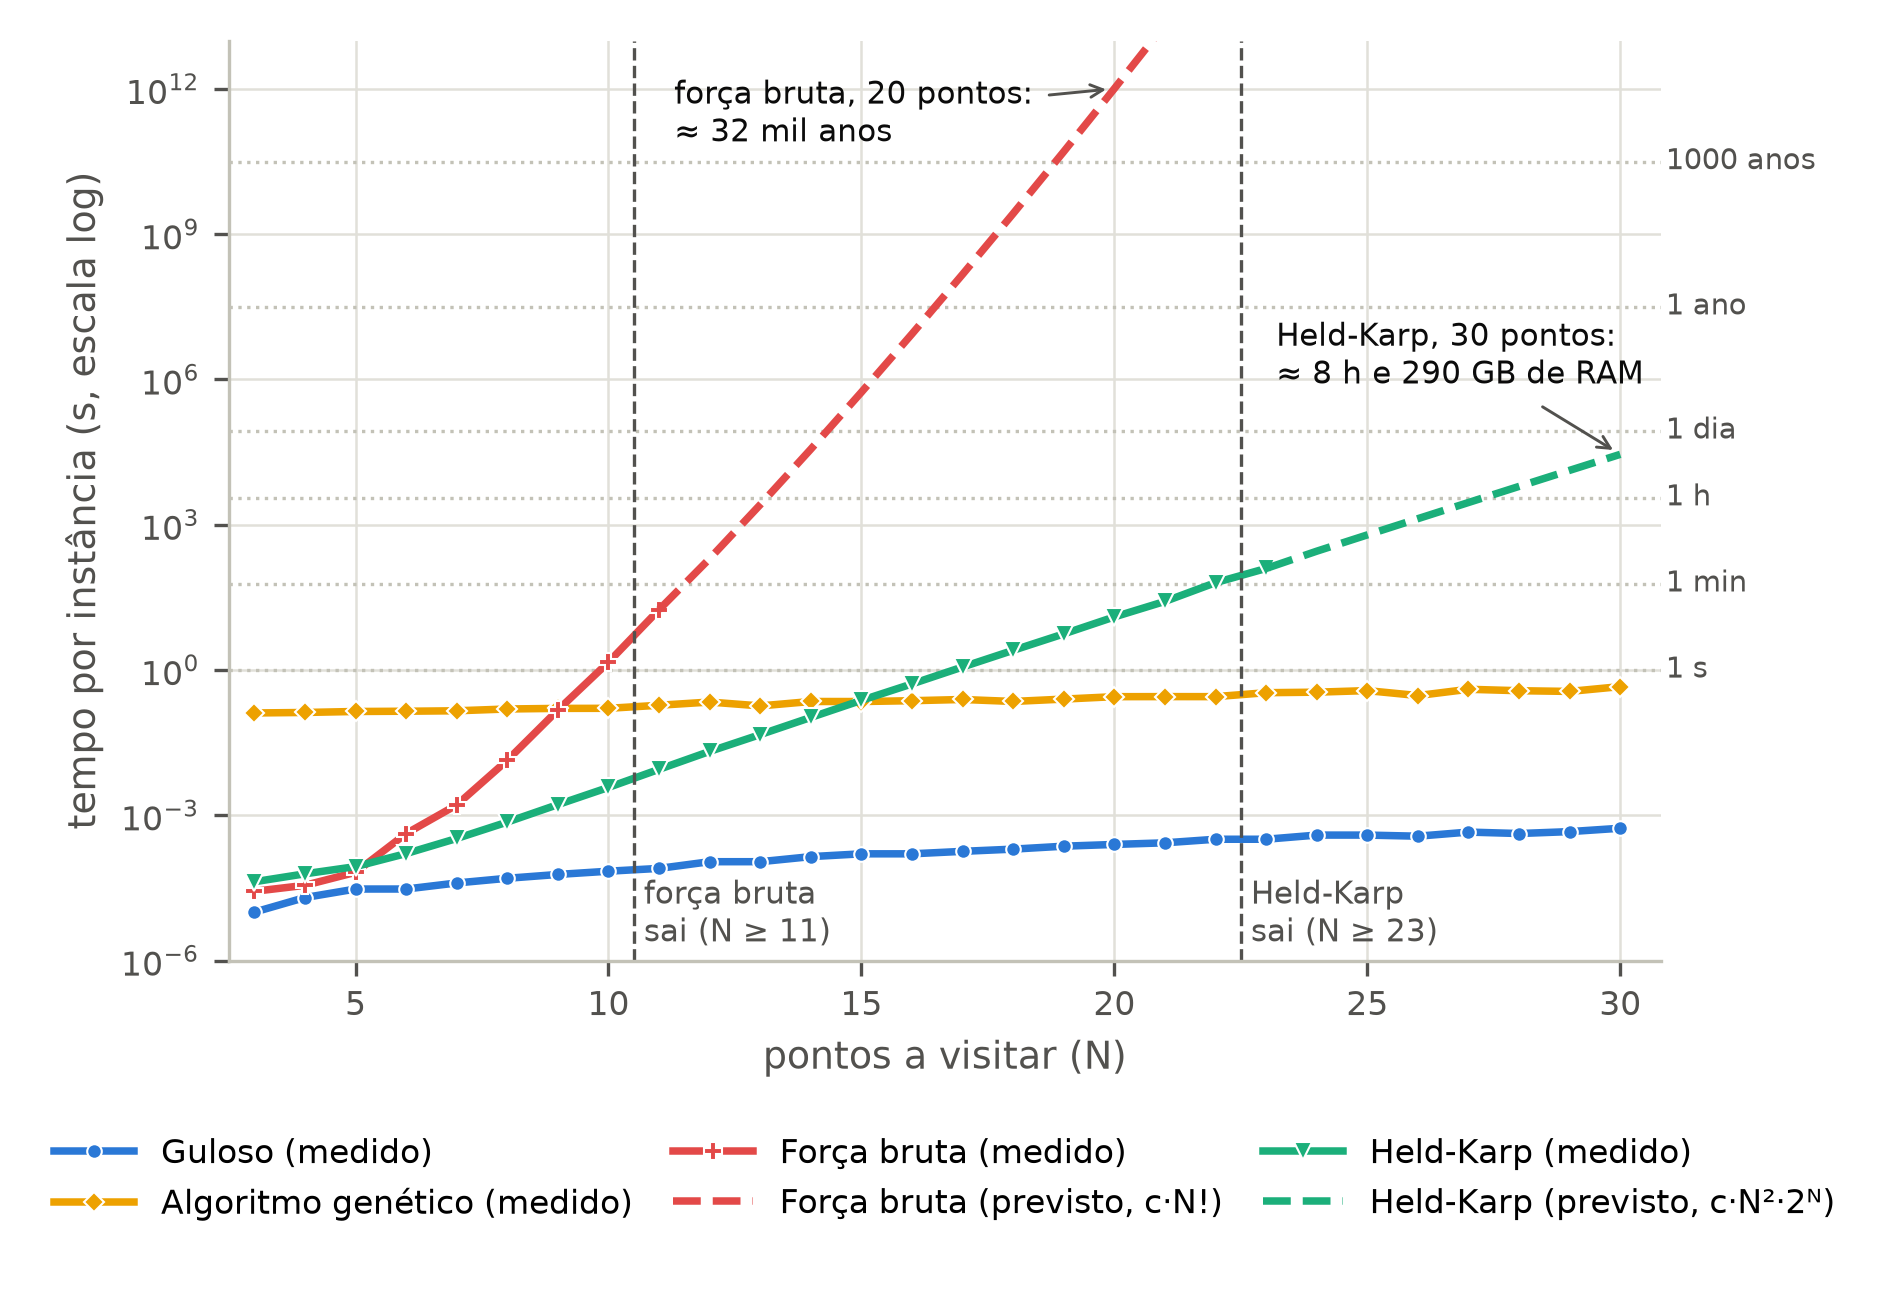
\includegraphics[width=\textwidth]{images/rotas/tempo_resolver.png}
    \fonte{elaborado pelos autores (2026).}
\end{figure}

\begin{figure}[H]
    \centering
    \caption{Memória necessária pelo Held-Karp e pelo algoritmo genético, por número de pontos.}
    \label{fig:rotas_memoria}
    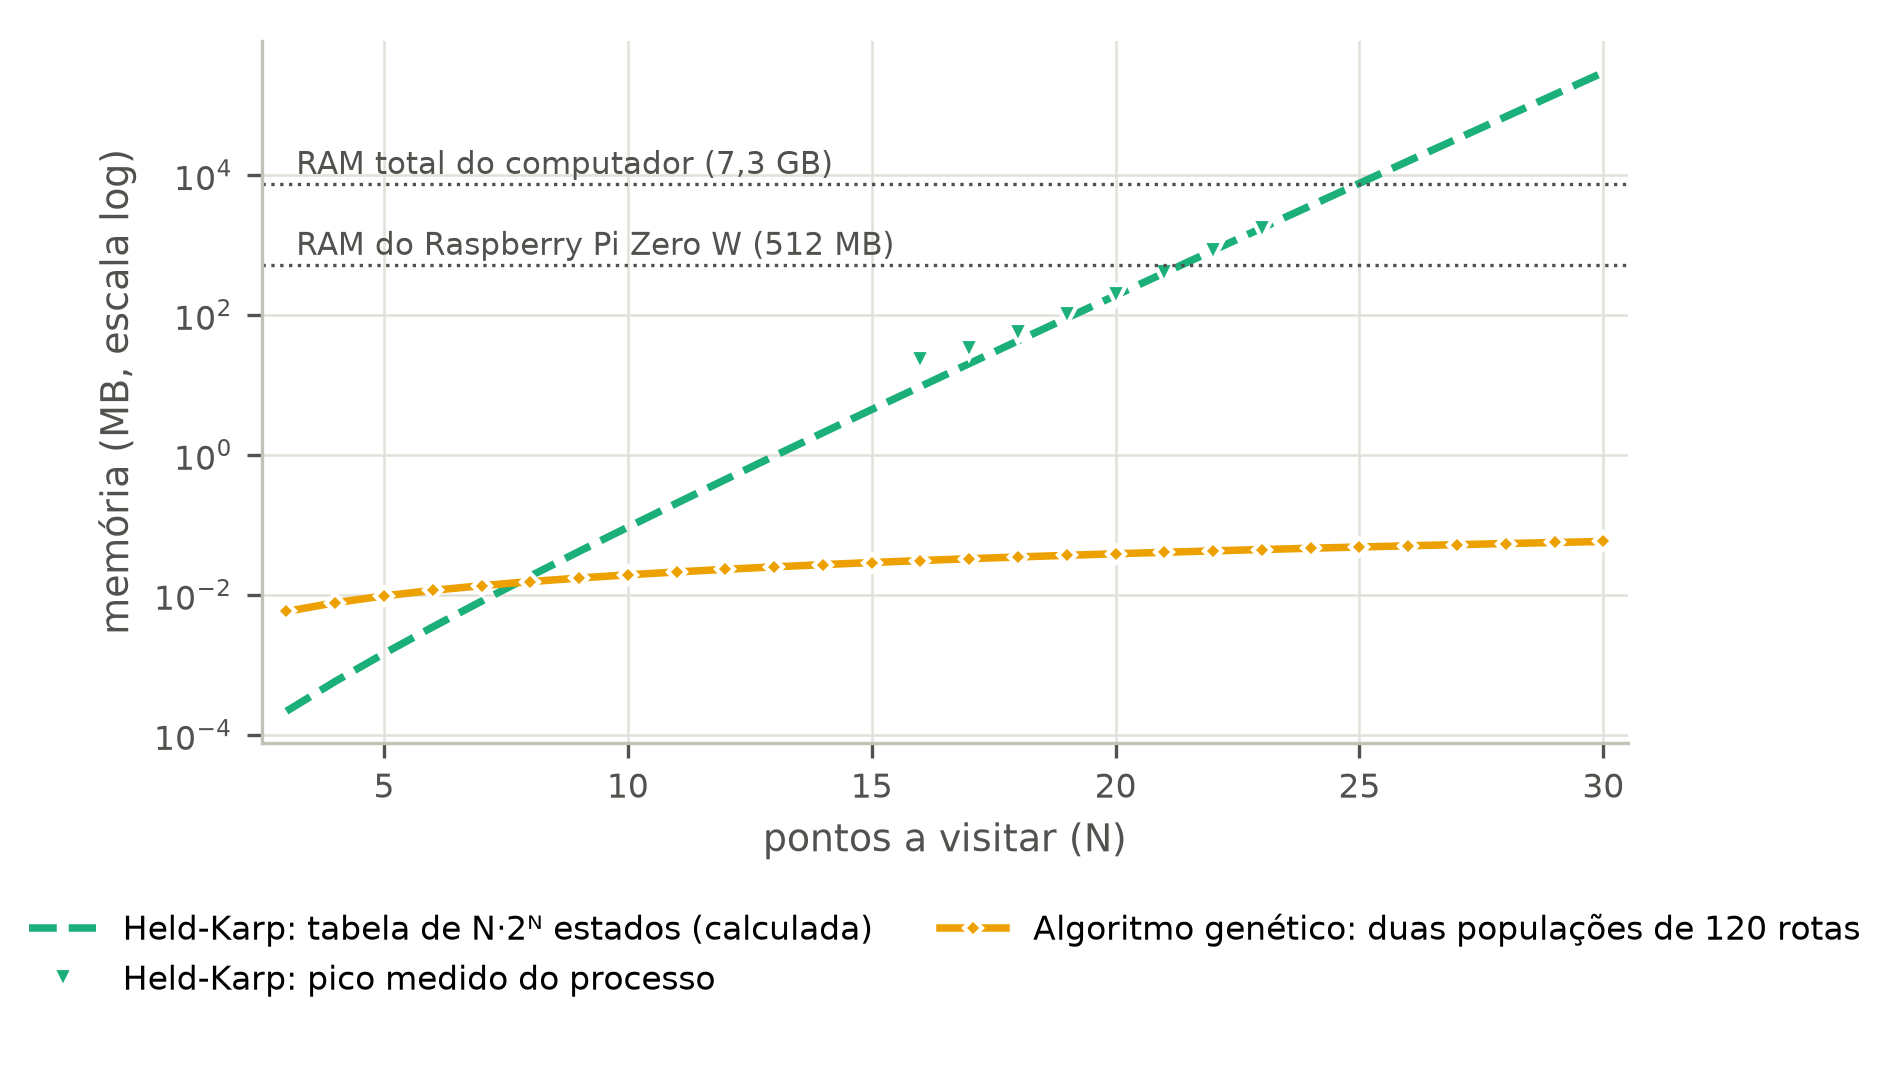
\includegraphics[width=\textwidth]{images/rotas/memoria_exato.png}
    \fonte{elaborado pelos autores (2026).}
\end{figure}

Com o critério da Seção~\ref{subsubsec:rotas_viabilidade}, cada método exato deixa o comparativo em um ponto diferente, o que divide os resultados em três faixas (Tabela~\ref{tab:rotas_fases}). Nas 80 instâncias em que os dois métodos exatos rodaram, os custos coincidiram em todas, o que confirma a implementação do Held-Karp.

\begin{table}[H]
    \centering
    \caption{Algoritmos executados em cada faixa de número de pontos.}
    \label{tab:rotas_fases}
    \small
    \renewcommand{\arraystretch}{1.25}
    \begin{tabular}{cccccc}
        \hline
        \textbf{Pontos ($N$)} & \textbf{Aleatório} & \textbf{Guloso} & \textbf{AG} & \textbf{Força bruta} & \textbf{Held-Karp} \\
        \hline
        3 a 10 & sim & sim & sim & sim & sim \\
        11 a 22 & sim & sim & sim & não & sim \\
        23 a 30 & sim & sim & sim & não & não \\
        \hline
    \end{tabular}
    \par\vspace{0.15cm}
    \footnotesize A força bruta sai com 11 pontos (18~s por instância e $\approx$ 3~min com 12); o Held-Karp sai com 23 (mais de 2~min e 1,7~GB) e não cabe na memória a partir de 25.\\
    Fonte: elaborado pelos autores (2026).
\end{table}

% ----------------------------------------------------------------
\subsection{Qualidade das rotas}\label{subsec:res_rotas_qualidade}
% ----------------------------------------------------------------

A Figura~\ref{fig:rotas_qualidade} apresenta a qualidade média das rotas, isto é, a razão entre o comprimento da rota de referência e o da rota obtida: 100\% corresponde à rota ótima (ou à melhor conhecida, acima de 22 pontos), e quanto maior o valor, melhor a rota. O AG manteve qualidade entre 96,5\% e 100\% em toda a faixa, o guloso entre 85\% e 94\%, e a ordem aleatória caiu de 74\% para 33\% com o aumento de $N$. As distâncias médias correspondentes estão na Tabela~\ref{tab:rotas_distancia}.

\begin{figure}[H]
    \centering
    \caption{Qualidade média das rotas, em relação à rota ótima ou à melhor conhecida (10 instâncias por $N$).}
    \label{fig:rotas_qualidade}
    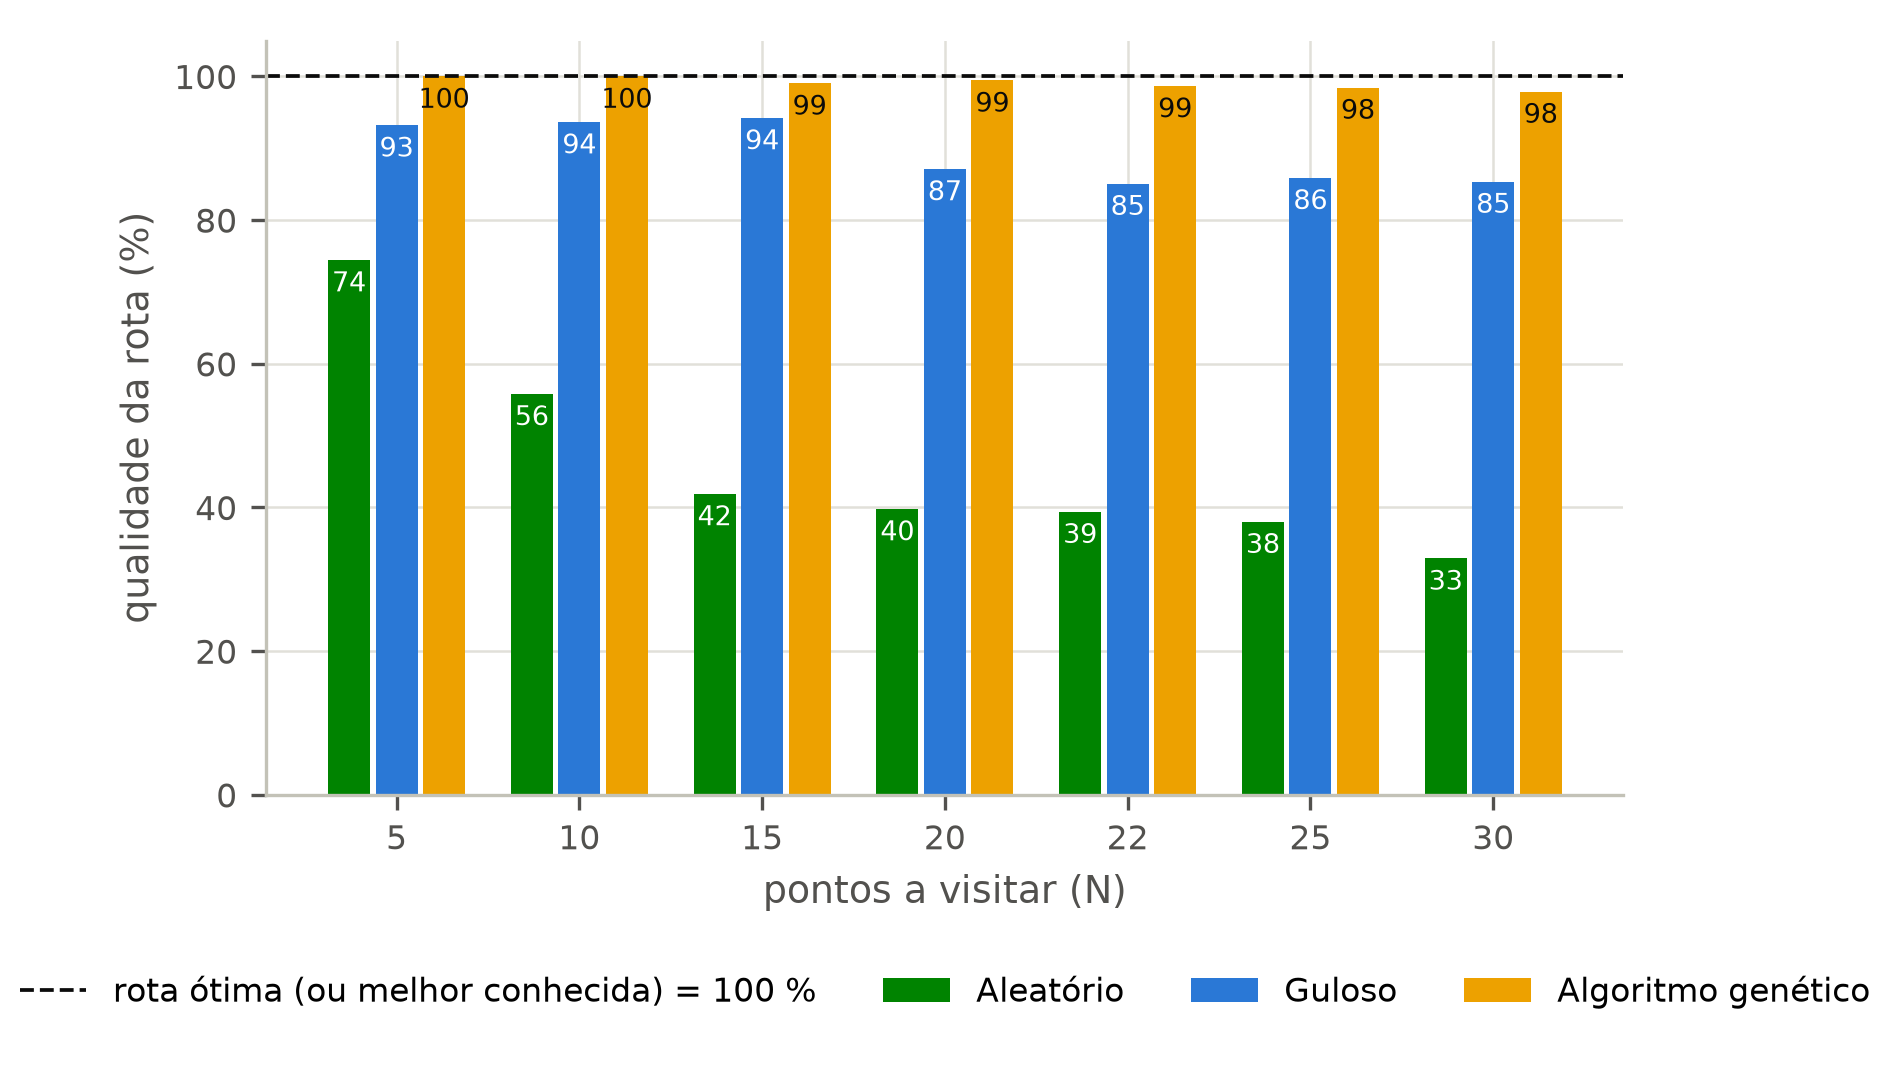
\includegraphics[width=\textwidth]{images/rotas/qualidade_rotas.png}
    \fonte{elaborado pelos autores (2026).}
\end{figure}

\begin{table}[H]
    \centering
    \caption{Distância média do circuito, em metros (10 instâncias por $N$).}
    \label{tab:rotas_distancia}
    \small
    \renewcommand{\arraystretch}{1.2}
    \begin{tabular}{cccccc}
        \hline
        \textbf{$N$} & \textbf{Aleatório} & \textbf{Guloso} & \textbf{AG} & \textbf{Força bruta} & \textbf{Held-Karp} \\
        \hline
        5 & 18,86 & 14,86 & 13,78 & 13,78 & 13,78 \\
        10 & 35,59 & 21,04 & 19,64 & 19,64 & 19,64 \\
        15 & 54,52 & 24,26 & 22,98 & --- & 22,76 \\
        20 & 65,12 & 29,82 & 25,94 & --- & 25,79 \\
        22 & 68,38 & 31,91 & 27,30 & --- & 26,93 \\
        25 & 77,76 & 34,34 & 29,76 & --- & --- \\
        30 & 98,44 & 38,04 & 32,96 & --- & --- \\
        \hline
    \end{tabular}
    \par\vspace{0.2cm}
    \footnotesize Fonte: elaborado pelos autores (2026).
\end{table}

A Tabela~\ref{tab:rotas_gap} agrupa o \textit{gap} e os acertos por faixa. Até 10 pontos, o AG obteve o ótimo global em todas as 80 instâncias; entre 11 e 22, em 70 de 120, com \textit{gap} médio de 0,85\%; entre 23 e 30, ficou em média 2,2\% acima da melhor rota conhecida. O guloso perdeu de 6,6\% a 18,3\% em média, chegando a 37\% em instâncias desfavoráveis.

\begin{table}[H]
    \centering
    \caption{\textit{Gap} médio, \textit{gap} máximo e acertos da referência, por faixa de $N$.}
    \label{tab:rotas_gap}
    \small
    \renewcommand{\arraystretch}{1.25}
    \setlength{\tabcolsep}{4pt}
    \begin{tabular}{lccc}
        \hline
        \textbf{Algoritmo} & \textbf{3 a 10 (ótimo)} & \textbf{11 a 22 (ótimo)} & \textbf{23 a 30 (melhor conhecida)} \\
        \hline
        Aleatório & 49,3\% (127,4\%) $\cdot$ 6/80 & 132,0\% (198,7\%) $\cdot$ 0/120 & 182,4\% (264,7\%) $\cdot$ 0/80 \\
        Guloso & 6,6\% (28,6\%) $\cdot$ 11/80 & 9,7\% (31,7\%) $\cdot$ 1/120 & 18,3\% (36,9\%) $\cdot$ 0/80 \\
        Algoritmo genético & 0,00\% (0,00\%) $\cdot$ 80/80 & 0,85\% (9,6\%) $\cdot$ 70/120 & 2,2\% (7,7\%) $\cdot$ 20/80 \\
        \hline
    \end{tabular}
    \par\vspace{0.15cm}
    \footnotesize Formato: \textit{gap} médio (\textit{gap} máximo) $\cdot$ instâncias em que a referência foi obtida.\\
    Fonte: elaborado pelos autores (2026).
\end{table}

A comparação instância a instância está na Tabela~\ref{tab:rotas_confronto}, em que cada célula indica em quantas das 280 instâncias o algoritmo da linha obteve rota mais curta que o da coluna. O AG superou o guloso em 262 instâncias e foi superado em 6; a ordem aleatória nunca superou o AG.

\begin{table}[H]
    \centering
    \caption{Instâncias, entre 280, em que o algoritmo da linha obteve rota mais curta que o da coluna.}
    \label{tab:rotas_confronto}
    \small
    \renewcommand{\arraystretch}{1.25}
    \begin{tabular}{lccc}
        \hline
        & \textbf{Aleatório} & \textbf{Guloso} & \textbf{AG} \\
        \hline
        \textbf{Aleatório} & --- & 9 & 0 \\
        \textbf{Guloso} & 270 & --- & 6 \\
        \textbf{AG} & 274 & 262 & --- \\
        \hline
    \end{tabular}
    \par\vspace{0.15cm}
    \footnotesize Empates (rotas de mesmo comprimento): aleatório e guloso, 1; aleatório e AG, 6; guloso e AG, 12.\\
    Fonte: elaborado pelos autores (2026).
\end{table}

As Figuras~\ref{fig:rotas_3d_n10} a \ref{fig:rotas_3d_n25} mostram as rotas em 3D de três instâncias. Com 10 e 20 pontos, o Held-Karp fornece o ótimo global, e o AG obtém exatamente a mesma rota, enquanto o guloso fica 26,1\% e 30,7\% acima, respectivamente. Com 25 pontos, o Held-Karp não pode ser executado, e o ótimo global é desconhecido. É nesse cenário que o \textit{benchmark} se mostra necessário: como o AG obteve o ótimo ou ficou próximo dele em todas as faixas em que o ótimo era conhecido, sua rota de 30,35~m é adotada como solução de referência prática, contra 34,14~m do guloso e 89,61~m da ordem aleatória.

\begin{figure}[H]
    \centering
    \caption{Rotas de 10 pontos obtidas pelos quatro algoritmos.}
    \label{fig:rotas_3d_n10}
    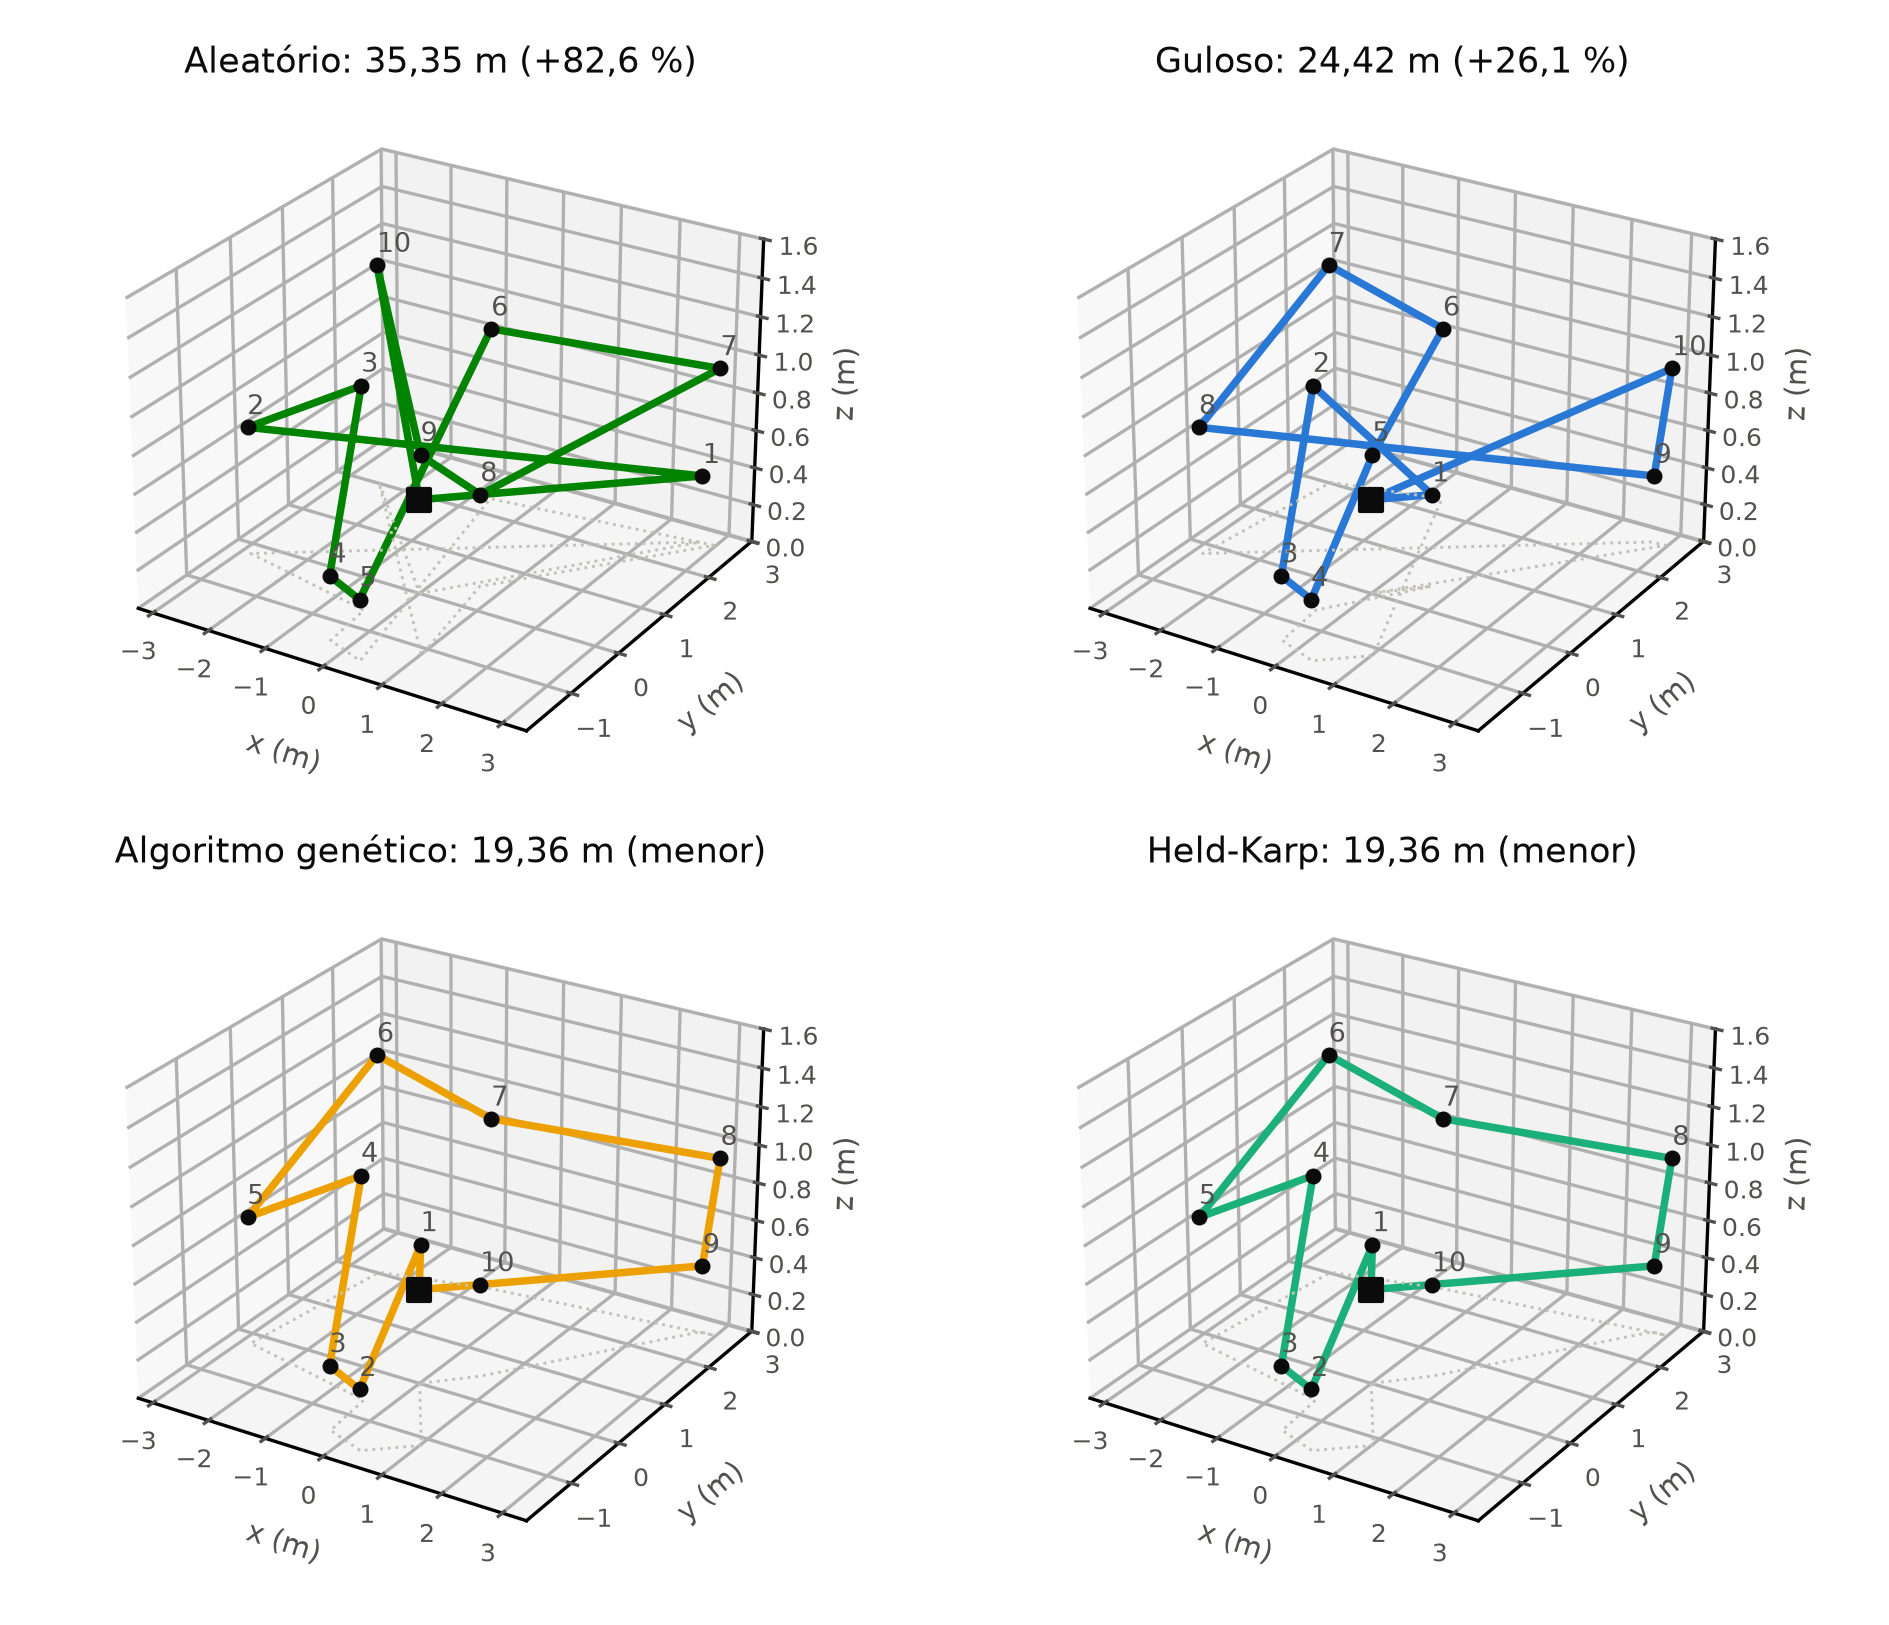
\includegraphics[width=\textwidth]{images/rotas/rotas_3d_n10.png}
    \fonte{elaborado pelos autores (2026).}
\end{figure}

\begin{figure}[H]
    \centering
    \caption{Rotas de 20 pontos obtidas pelos quatro algoritmos.}
    \label{fig:rotas_3d_n20}
    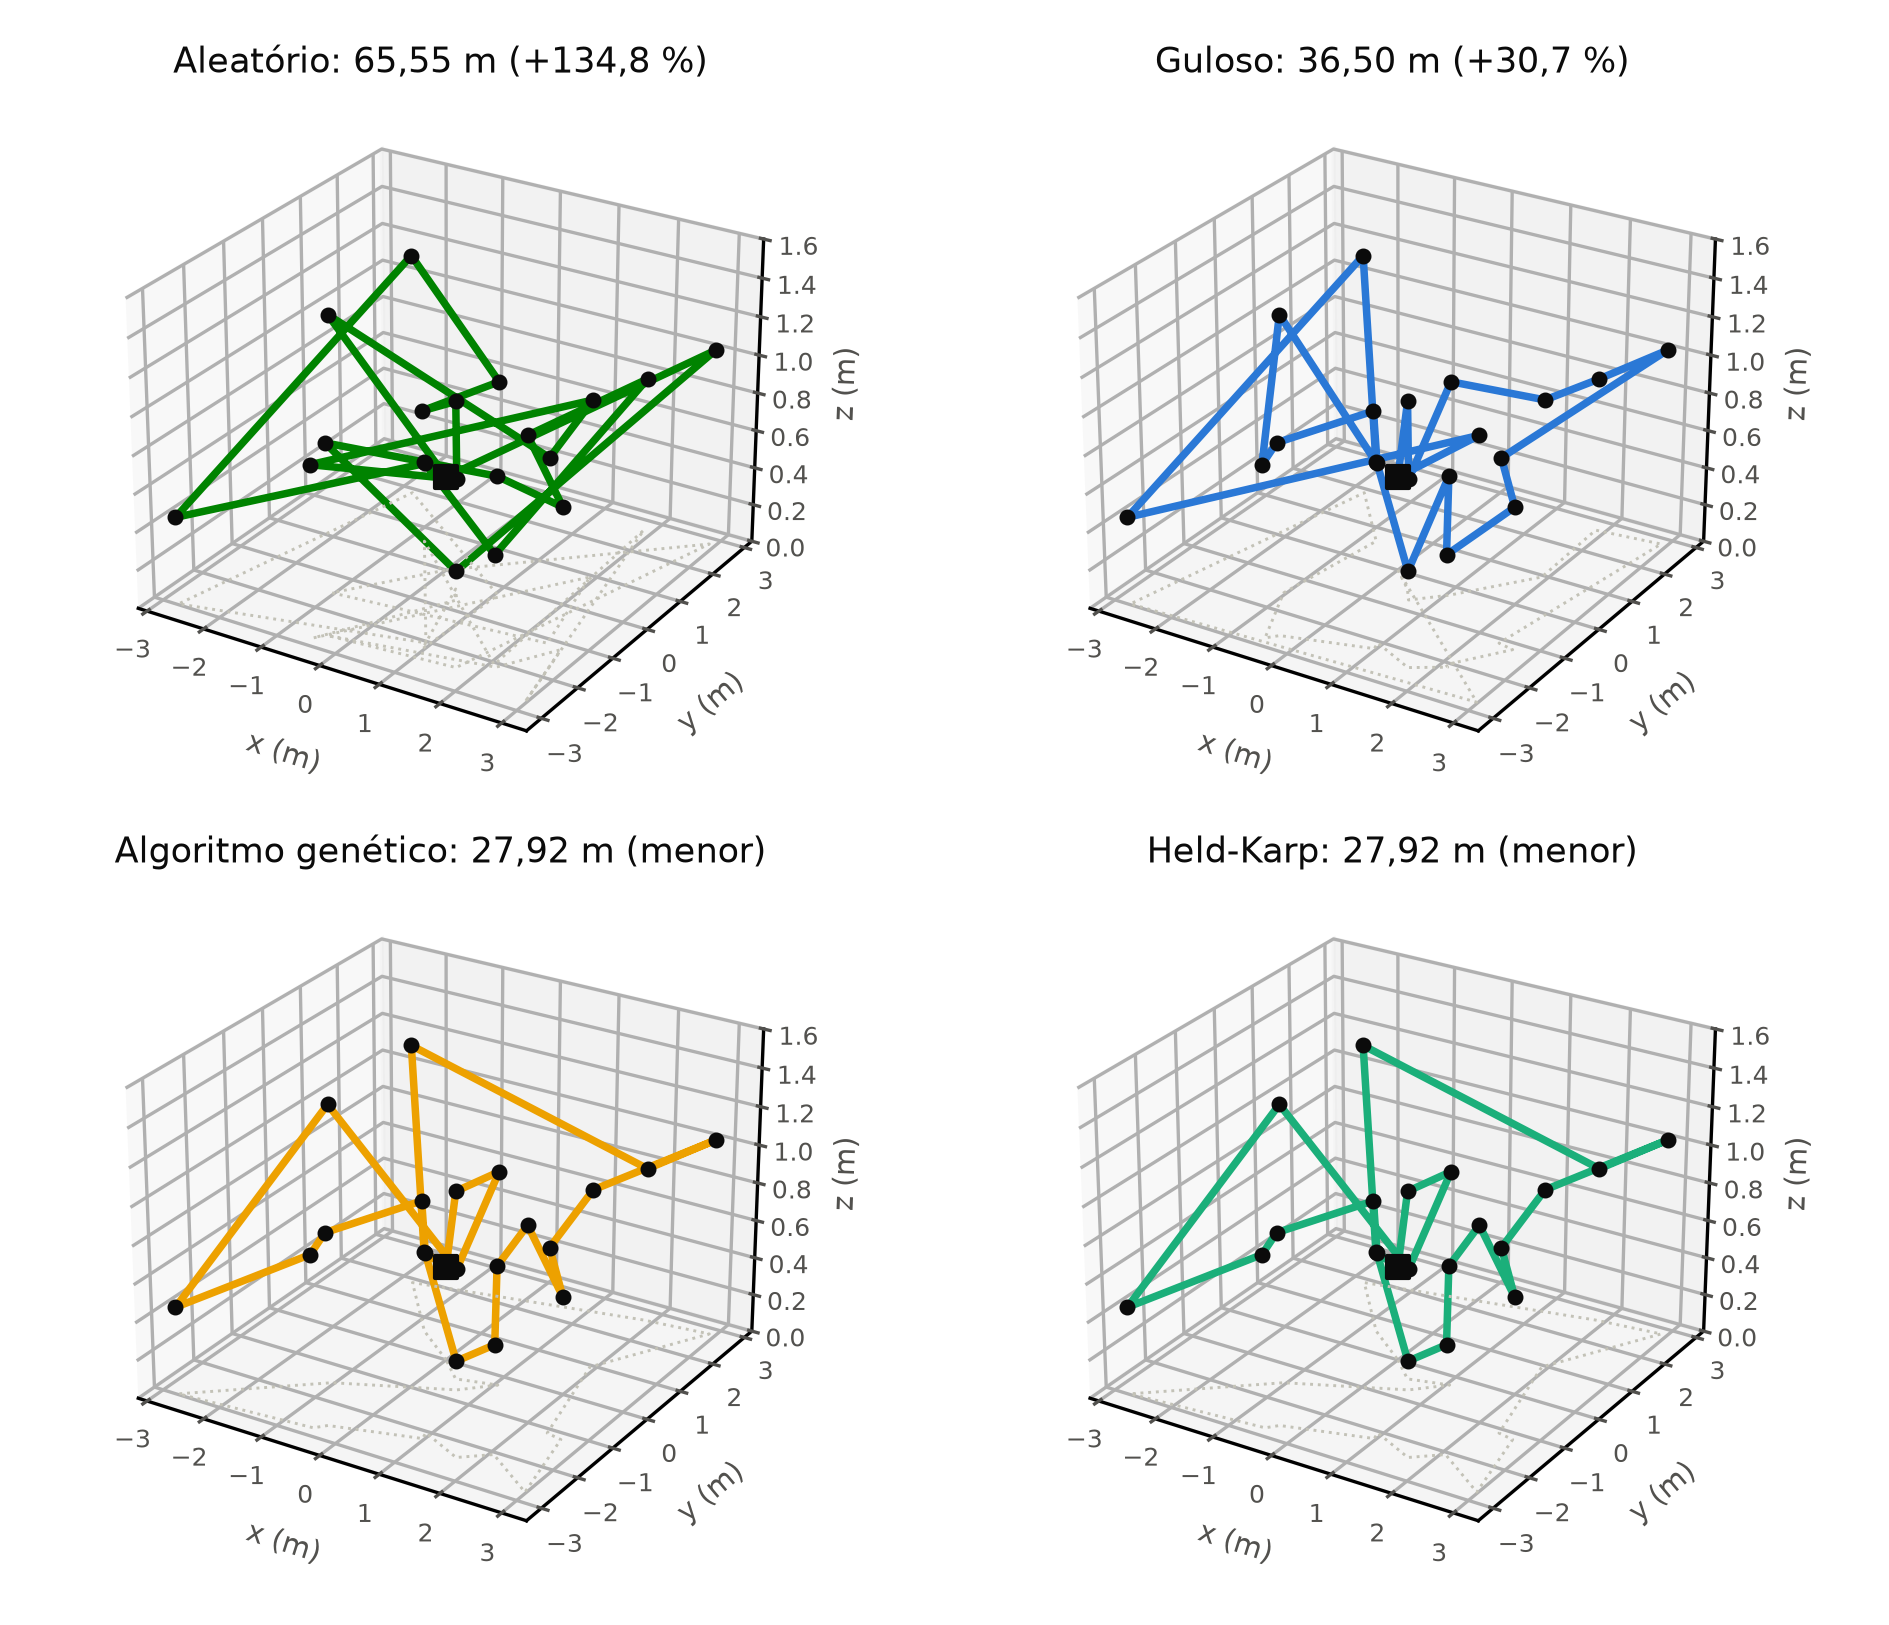
\includegraphics[width=\textwidth]{images/rotas/rotas_3d_n20.png}
    \fonte{elaborado pelos autores (2026).}
\end{figure}

\begin{figure}[H]
    \centering
    \caption{Rotas de 25 pontos, em que o Held-Karp não cabe na memória do computador.}
    \label{fig:rotas_3d_n25}
    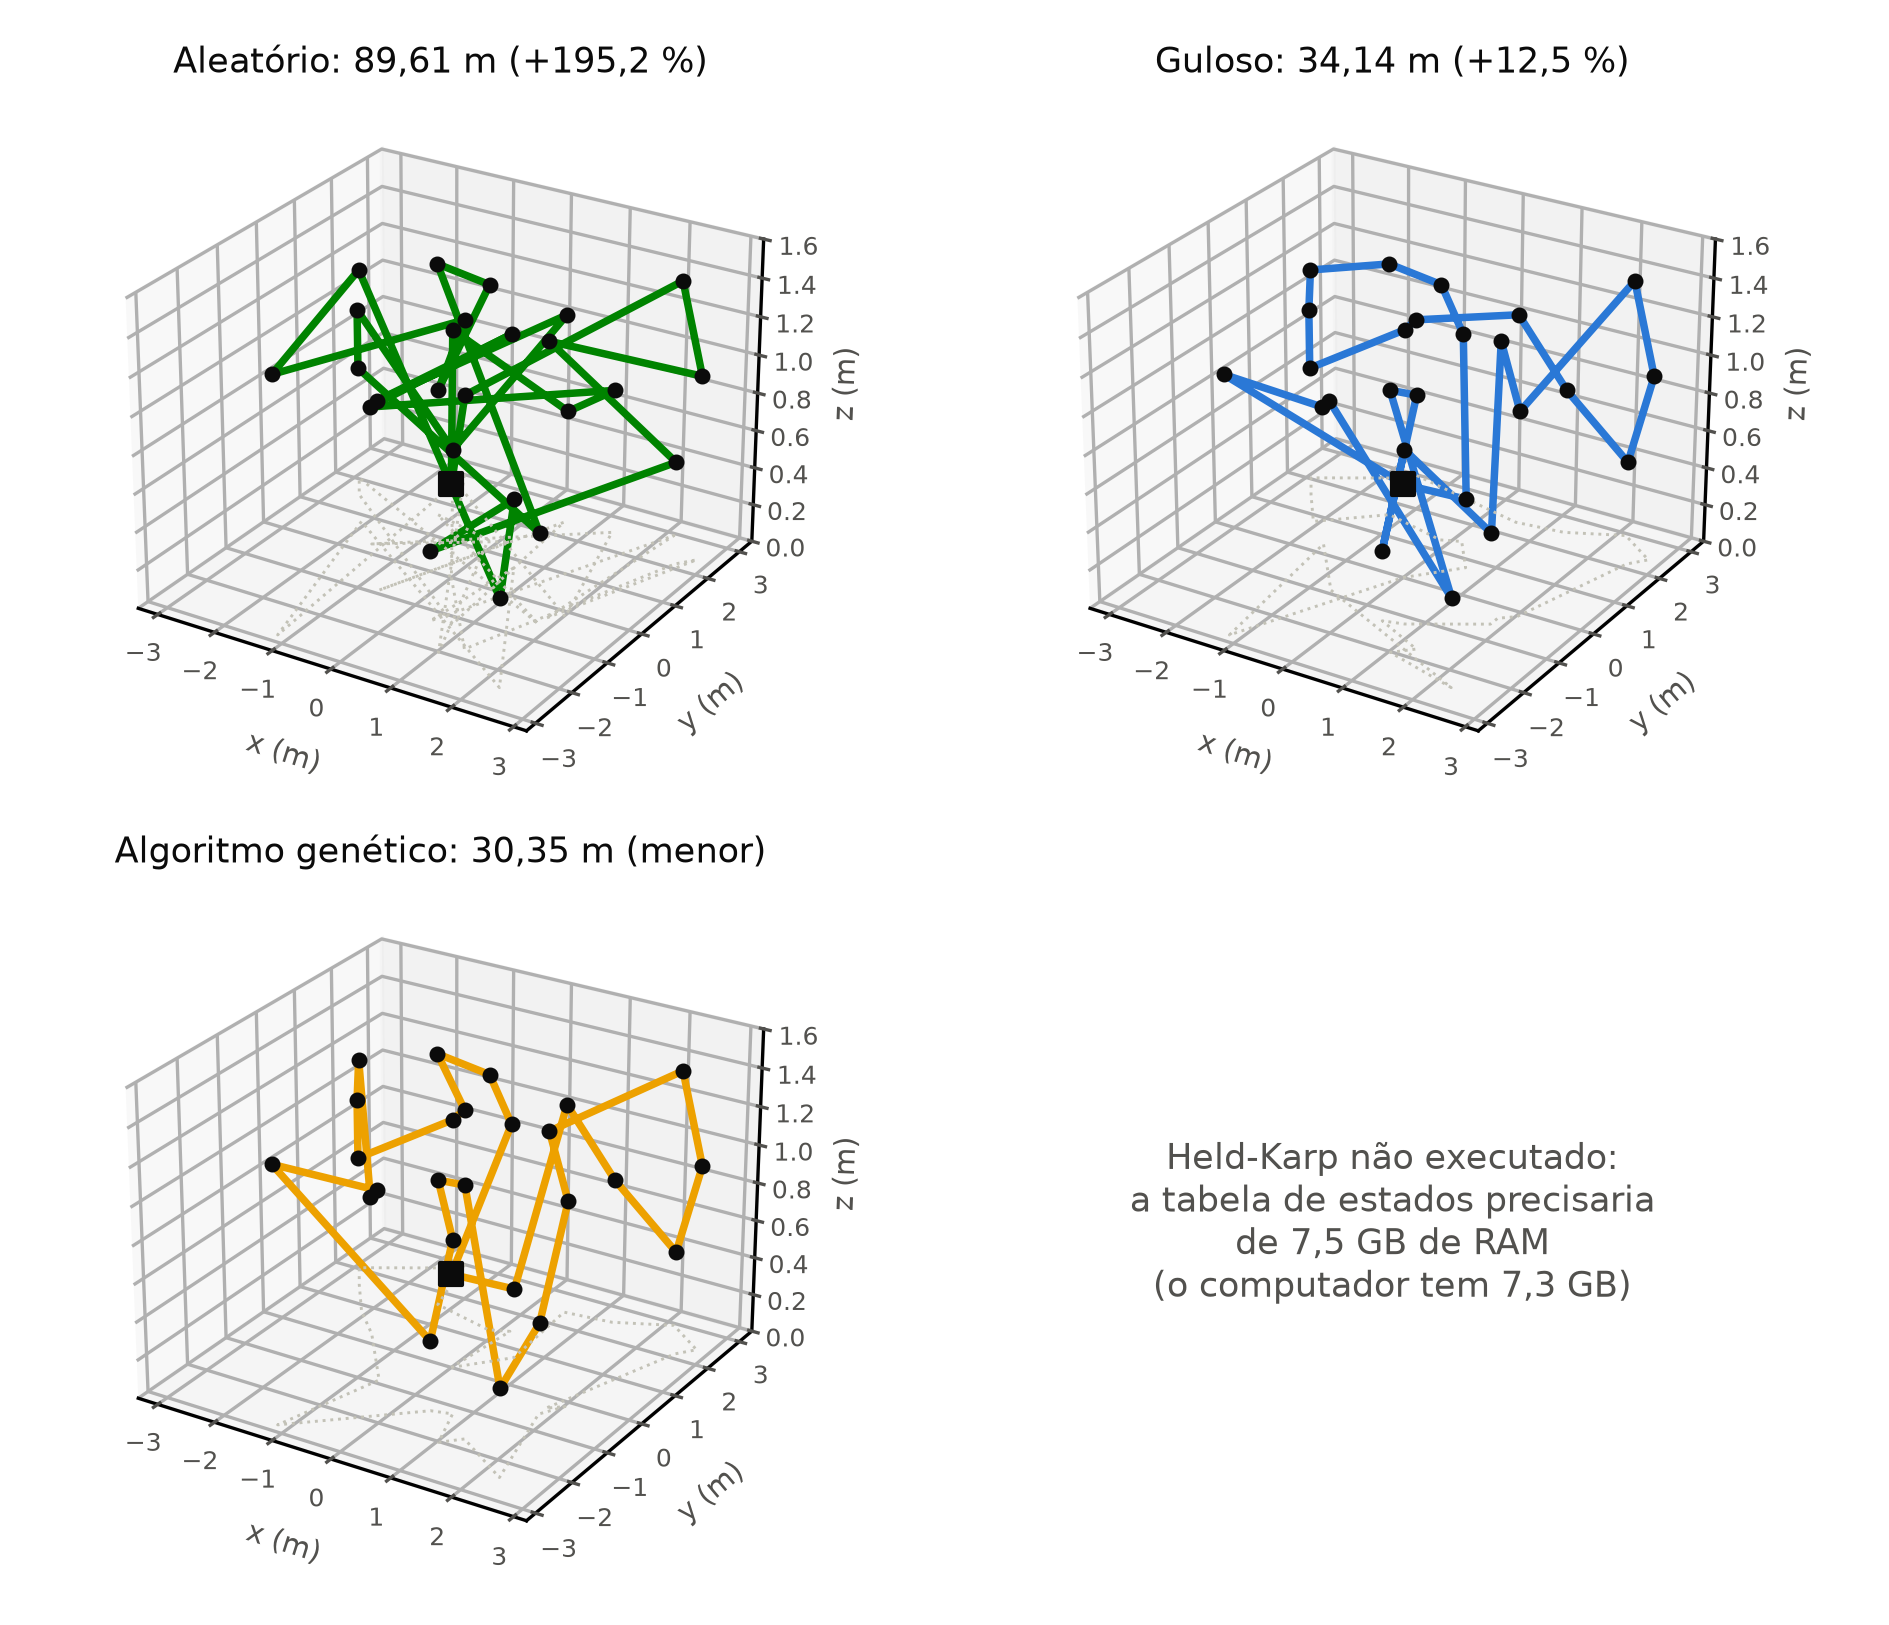
\includegraphics[width=\textwidth]{images/rotas/rotas_3d_n25.png}
    \fonte{elaborado pelos autores (2026).}
\end{figure}

% ----------------------------------------------------------------
\subsection{Tempo de cálculo}\label{subsec:res_rotas_tempo}
% ----------------------------------------------------------------

A Tabela~\ref{tab:rotas_tempo} apresenta o tempo médio de cálculo por instância no \textit{benchmark}. O AG levou de 0,13 a 0,45~s em toda a faixa, valor dominado pelo número de gerações (média de 272, mínimo de 200 e máximo de 665) e pouco sensível a $N$. A força bruta já é mais lenta que o AG com 10 pontos, e o Held-Karp, a partir de 15. Os tempos variaram cerca de 10\% entre execuções repetidas, conforme a carga do computador; as rotas e distâncias não se alteraram.

\begin{table}[H]
    \centering
    \caption{Tempo médio de cálculo por instância.}
    \label{tab:rotas_tempo}
    \small
    \renewcommand{\arraystretch}{1.2}
    \begin{tabular}{ccccc}
        \hline
        \textbf{$N$} & \textbf{Guloso} & \textbf{AG} & \textbf{Força bruta} & \textbf{Held-Karp} \\
        \hline
        5 & 0,03~ms & 139~ms & 0,06~ms & 0,07~ms \\
        10 & 0,07~ms & 162~ms & 1,56~s & 4,1~ms \\
        15 & 0,16~ms & 223~ms & --- & 260~ms \\
        20 & 0,25~ms & 281~ms & --- & 13,0~s \\
        22 & 0,32~ms & 282~ms & --- & 63,7~s \\
        25 & 0,39~ms & 376~ms & --- & --- \\
        30 & 0,54~ms & 454~ms & --- & --- \\
        \hline
    \end{tabular}
    \par\vspace{0.2cm}
    \footnotesize Fonte: elaborado pelos autores (2026).
\end{table}

% ----------------------------------------------------------------
\subsection{Convergência do algoritmo genético}\label{subsec:res_rotas_convergencia}
% ----------------------------------------------------------------

A Figura~\ref{fig:rotas_convergencia} mostra a evolução do melhor indivíduo do AG na primeira instância de quatro valores de $N$. A população inicial, aleatória, começa entre 35\% e 150\% acima da referência e melhora rapidamente nas primeiras 50 a 150 gerações, superando o guloso. Depois, a melhora cessa: com 10 e 20 pontos o AG atingiu o ótimo global, mas com 15 pontos estabilizou 3,4\% acima dele (24,27~m contra 23,47~m), preso em um ótimo local, isto é, uma rota que as operações do AG não conseguiram mais encurtar, embora existisse uma rota menor.

\begin{figure}[H]
    \centering
    \caption{Convergência do melhor indivíduo do algoritmo genético.}
    \label{fig:rotas_convergencia}
    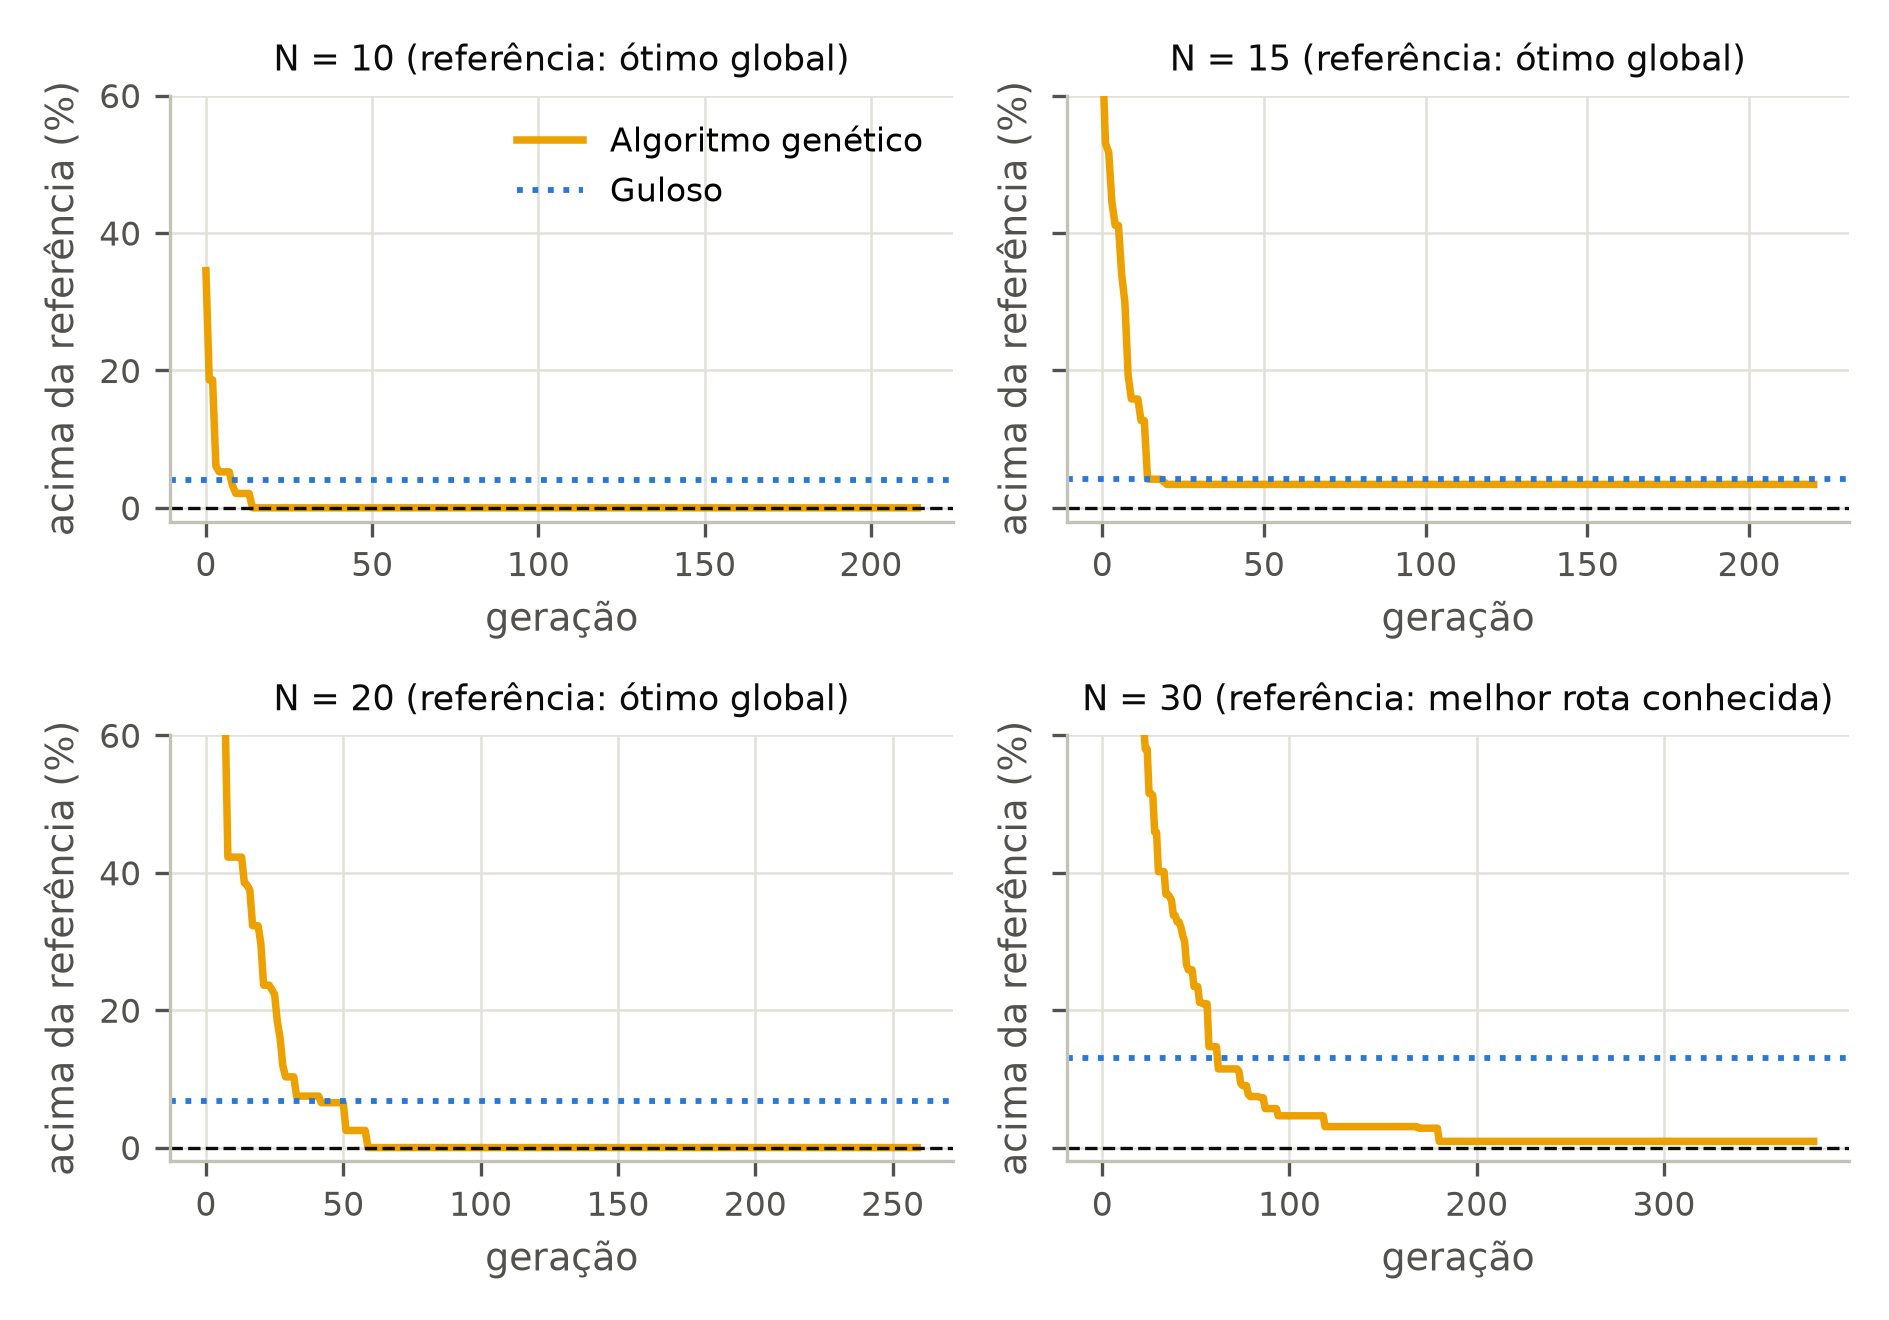
\includegraphics[width=\textwidth]{images/rotas/convergencia_genetico.png}
    \fonte{elaborado pelos autores (2026).}
\end{figure}

% ----------------------------------------------------------------
\subsection{Investigação complementar: busca local 2-opt}\label{subsec:res_rotas_2opt}
% ----------------------------------------------------------------

Durante o desenvolvimento, identificou-se na literatura que a busca local repetida a partir de várias rotas iniciais é uma alternativa competitiva para o TSP \cite{johnson1997}. Por isso, a busca local 2-opt com 20 partidas aleatórias foi incluída no \textit{benchmark} de forma exploratória, sem estudo aprofundado de seus parâmetros. A Tabela~\ref{tab:rotas_2opt} compara seus resultados com os do AG.

\begin{table}[H]
    \centering
    \caption{Comparação exploratória entre o AG e a busca local 2-opt com 20 partidas.}
    \label{tab:rotas_2opt}
    \small
    \renewcommand{\arraystretch}{1.25}
    \begin{tabular}{lcc}
        \hline
        \textbf{Indicador} & \textbf{AG} & \textbf{2-opt com 20 partidas} \\
        \hline
        Ótimo global obtido (instâncias de até 22 pontos) & 150 de 200 & 189 de 200 \\
        \textit{Gap} médio entre 11 e 22 pontos & 0,85\% & 0,04\% \\
        \textit{Gap} médio entre 23 e 30 pontos & 2,2\% & 0,05\% \\
        Tempo médio com 30 pontos & 454~ms & 16~ms \\
        Rota mais curta que a do outro (280 instâncias) & 8 & 106 \\
        \hline
    \end{tabular}
    \par\vspace{0.15cm}
    \footnotesize As 166 instâncias restantes terminaram empatadas.\\
    Fonte: elaborado pelos autores (2026).
\end{table}

Nos dados obtidos, a busca local com múltiplas partidas foi superior ao AG em qualidade e cerca de 30 vezes mais rápida. A análise das partidas ajuda a explicar o resultado: com 30 pontos, as 20 partidas convergiram em média para 18 ótimos locais diferentes, e somente 5,5\% delas alcançaram a melhor rota. Uma única busca local, portanto, fica facilmente presa em um ótimo local, mas repeti-la a partir de pontos de partida diferentes aumenta muito a chance de alcançar o ótimo global. Verificou-se também que 277 das 280 rotas do AG já eram ótimos locais em relação ao 2-opt; ou seja, o AG encontra ótimos locais com frequência, mas nem sempre o global. Como essa abordagem não foi estudada em profundidade, ela é indicada como alternativa a ser explorada em trabalhos futuros.

% ----------------------------------------------------------------
\subsection{Execução das rotas no controlador de voo}\label{subsec:res_rotas_stm32}
% ----------------------------------------------------------------

As rotas de uma instância tridimensional de 6 pontos, com alturas de 64 a 145~cm, foram executadas pelo STM32 com o VANT simulado, conforme a Seção~\ref{subsubsec:rotas_execucao_stm32} (Tabela~\ref{tab:rotas_stm32}). O AG obteve a mesma rota do Held-Karp percorrida no sentido inverso, com o mesmo comprimento, 21,3\% menor que a do guloso. Em todas as execuções, o VANT simulado chegou a cada ponto com erro máximo de 3,1~cm, dentro da tolerância de 5~cm usada pelo STM32 para declarar estabilidade.

\begin{table}[H]
    \centering
    \caption{Rotas tridimensionais executadas pelo STM32 com o VANT simulado.}
    \label{tab:rotas_stm32}
    \small
    \renewcommand{\arraystretch}{1.2}
    \begin{tabular}{ccccc}
        \hline
        \textbf{Algoritmo} & \textbf{Ordem} & \textbf{Circuito 3D} & \textbf{Trechos executados} & \textbf{Maior erro em um ponto} \\
        \hline
        Guloso & 3 4 5 2 1 6 & 1898~cm & 14 & 3,0~cm \\
        AG & 3 4 6 5 2 1 & 1493~cm ($-21{,}3\%$) & 14 & 3,0~cm \\
        Held-Karp & 1 2 5 6 4 3 & 1493~cm ($-21{,}3\%$) & 14 & 3,1~cm \\
        \hline
    \end{tabular}
    \par\vspace{0.15cm}
    \footnotesize Pontos (cm): $(-177, 188, 129)$, $(-104, -150, 145)$, $(43, -43, 99)$, $(62, -71, 64)$, $(92, -204, 93)$ e $(298, -274, 134)$.\\
    Fonte: elaborado pelos autores (2026).
\end{table}

% ----------------------------------------------------------------
\subsection{Execução do algoritmo genético no Raspberry Pi Zero W}\label{subsec:res_rotas_pi}
% ----------------------------------------------------------------

A Tabela~\ref{tab:rotas_pi} compara a rota obtida pelo AG no computador pessoal e no Raspberry Pi Zero W para três instâncias: o quadrado de 40~cm executado com o VANT simulado no STM32 no ensaio de comunicação (Seção~\ref{subsec:res_com_missao}) e duas instâncias do \textit{benchmark}, com 10 e 30 pontos. Nas três, a ordem, o comprimento e a assinatura SHA-256 foram idênticos nas duas máquinas: o Raspberry Pi calcula exatamente a mesma rota, e os resultados de qualidade do \textit{benchmark} valem para o algoritmo embarcado. Os 26 testes automatizados do programa também foram aprovados no próprio Raspberry Pi.

\begin{table}[H]
    \centering
    \caption{Mesma rota calculada pelo AG no computador pessoal e no Raspberry Pi Zero W.}
    \label{tab:rotas_pi}
    \small
    \renewcommand{\arraystretch}{1.2}
    \begin{tabular}{lccccc}
        \hline
        \textbf{Instância} & \textbf{Comprimento} & \textbf{SHA-256} & \textbf{PC} & \textbf{Raspberry Pi} & \textbf{Razão} \\
        \hline
        Quadrado de 40~cm & 160,0~cm & \texttt{52d2b0c4\ldots} & 0,14~s & 9,70~s & 69$\times$ \\
        10 pontos & 19,36~m & \texttt{9ffc5830\ldots} & 0,16~s & 11,14~s & 70$\times$ \\
        30 pontos & 30,84~m & \texttt{11f260a1\ldots} & 0,39~s & 23,92~s & 61$\times$ \\
        \hline
    \end{tabular}
    \par\vspace{0.15cm}
    \footnotesize A assinatura é a mesma nas duas máquinas; são mostrados os 8 primeiros dígitos hexadecimais. Tempos de uma execução de cada instância.\\
    Fonte: elaborado pelos autores (2026).
\end{table}

O Raspberry Pi foi de 61 a 70 vezes mais lento, levando de 10 a 24~s para ordenar de 3 a 30 pontos. Como a ordem é calculada uma única vez, antes da execução da rota, e cada trecho leva vários segundos para ser voado, esse tempo é aceitável para a aplicação. Os métodos exatos, por outro lado, seriam ainda mais limitados na placa: além de dezenas de vezes mais lentos, o Held-Karp ultrapassa metade dos 512~MB de RAM a partir de 21 pontos (Seção~\ref{subsec:res_rotas_limite}).

% ----------------------------------------------------------------
\subsection{Discussão}\label{subsec:res_rotas_discussao}
% ----------------------------------------------------------------

Os resultados confirmam que a obtenção do ótimo global se torna inviável com poucas dezenas de pontos, mesmo com o melhor dos métodos exatos avaliados. A força bruta, que traduz diretamente a definição do problema, deixa de ser praticável com 11 pontos. O Held-Karp estende esse limite para 22 pontos, sendo cerca de $10^{11}$ vezes mais rápido que a força bruta com 20 pontos, ao custo de uma tabela de estados que dobra a cada ponto adicionado; com 25 pontos, a memória necessária excede a do computador utilizado e, no Raspberry Pi Zero W, o limite é ainda menor.

O algoritmo genético manteve tempo inferior a 0,5~s e memória inferior a 0,1~MB em toda a faixa, com rotas iguais ao ótimo até 10 pontos e, em média, até 3,7\% acima da referência nas faixas maiores. Isso o torna viável exatamente onde os métodos exatos deixam de ser, e o \textit{benchmark} nas faixas em que o ótimo é conhecido fundamenta o uso de sua rota quando o ótimo não pode ser calculado. O guloso, embora mais rápido, perdeu de 6\% a 18\% de distância em média, e a ordem aleatória chegou a três vezes o comprimento ótimo.

No Raspberry Pi Zero W, o mesmo AG produziu exatamente as mesmas rotas, com tempo de 10 a 24~s, de 60 a 70 vezes maior que no computador pessoal. Esses resultados sustentam a viabilidade do algoritmo genético como solução adotada e validada no projeto, com qualidade de rota e tempo de cálculo compatíveis com o planejamento antes do voo. A validação de sua execução no Raspberry Pi e da integração com o controlador de voo fundamenta sua utilização no protótipo, mas não demonstra superioridade em relação a todas as alternativas avaliadas.

Um limite deve ser considerado: o AG implementado não usa busca local, ou seja, não tenta encurtar as rotas por pequenas modificações sistemáticas, e pode estabilizar em um ótimo local, como observado com 15 pontos. A investigação complementar indicou que a busca local repetida obteve rotas melhores em menos tempo; combiná-la ao AG, formando um algoritmo memético \cite{moscato1989}, ou adotá-la diretamente são caminhos para trabalhos futuros.


\clearpage

\chapter{CONSIDERAÇÕES FINAIS}
\label{cap:conclusao}
No que tange ao sistema de controle e estabilização, os ensaios práticos evidenciaram que a abordagem LQR/LQG, em conjunto com o Filtro de Kalman linear, manteve a estabilidade de rolamento e arfagem do veículo. Em ensaios com o deslocamento horizontal restringido por um apoio físico, a altura de referência foi alcançada; em voo livre, porém, o veículo não manteve a posição nos eixos $X$ e $Y$ nem a guinada durante a subida. Essa deriva o expôs a forças externas do ambiente de ensaio, como cabos, paredes e correntes de ar, que provocaram a inclinação excessiva e o acionamento do sistema de segurança (\textit{failsafe}). A manutenção da posição horizontal mostrou-se, assim, o principal ponto a aperfeiçoar, pois expôs o impacto de perturbações não modeladas e de torques constantes gerados por assimetrias físicas.

Diante desses resultados, como trabalhos futuros na área de controle, sugere-se o aprimoramento das técnicas de modelagem matemática da planta, buscando uma representação que englobe efeitos aerodinâmicos e aproxime o modelo no espaço de estados do comportamento físico real. Recomenda-se também um rigor maior no projeto mecânico para garantir o balanceamento adequado da carga estrutural no drone, alinhando o centro de gravidade de modo a mitigar os torques parasitas. Por fim, propõe-se a adoção de técnicas de estimação de estados mais sofisticadas, substituindo o filtro linear pelo Filtro de Kalman Estendido (EKF -- \textit{Extended Kalman Filter}) baseado na cinemática de quatérnios. Em contraste com os ângulos de Euler tradicionais, o uso de quatérnios eliminaria as singularidades matemáticas (\textit{gimbal lock}) e reduziria substancialmente a carga de cálculos trigonométricos no microcontrolador, proporcionando uma fusão sensorial mais robusta, computacionalmente eficiente e adequada à dinâmica inerentemente não linear do VANT.
% Comunicação Raspberry Pi <-> STM32
% ============================================================================
% CONSIDERAÇÕES FINAIS — comunicação entre o Raspberry Pi e o STM32
% Chamado em partes/textuais/conclusao.tex.
% ============================================================================


Na comunicação entre o computador de missão e o controlador de voo, foi desenvolvido o DroneLink, protocolo de aplicação sobre o enquadramento MAVLink 2, definido em um único arquivo XML do qual são gerados os códigos do STM32 e do Raspberry Pi. O protocolo divide a missão em trechos executados um de cada vez: cada trecho é validado pelo STM32 antes de ser aceito, só é dado como concluído quando o VANT está estável no alvo e pode ser retransmitido com segurança, pois pedidos repetidos não são executados duas vezes. A identidade de \textit{boot} persistente impede a execução de comandos anteriores a uma reinicialização, e a supervisão do \textit{HEARTBEAT} e da autorização do operador leva o VANT a manter a posição e, em seguida, a pousar se o Raspberry Pi deixar de responder.

Sobre esse protocolo, o Raspberry Pi oferece ao operador comandos com a nomenclatura aeronáutica usual, entre eles o \texttt{route}, que ordena os pontos pelo algoritmo genético e executa a rota de forma automática. No ensaio integrado pela UART, com o VANT simulado no STM32, não foram registradas perdas nem erros de \textit{checksum} durante os 60~s de observação do enlace, com latência de ida e volta em torno de 10~ms; todas as recusas ocorreram com o motivo previsto; um pedido repetido foi executado uma única vez; a missão completa foi executada com erro máximo de 1,4~cm por ponto; e o STM32 manteve a posição em cerca de 1~s e iniciou o pouso entre 5,29 e 5,98~s diante da perda da autorização ou do encerramento do programa do Raspberry Pi. Os ensaios também permitiram identificar e corrigir seis falhas de integração, três delas visíveis somente com os dois lados conectados.

Como trabalhos futuros, recomenda-se realizar ensaios integrados com os motores em funcionamento, avaliando a comunicação sob vibração e interferência elétrica; reduzir o tempo de cálculo do algoritmo genético no Raspberry Pi Zero W; e avaliar a assinatura de mensagens do MAVLink 2 para autenticação da origem, especialmente caso a comunicação seja disponibilizada por rede sem fio.


% Planejamento de rotas
% ============================================================================
% CONSIDERAÇÕES FINAIS — planejamento de rotas
% Chamado em partes/textuais/conclusao.tex.
% ============================================================================

No planejamento de rotas, a ordem de visita dos pontos foi modelada como o Problema do Caixeiro Viajante com custo igual à distância tridimensional do circuito, que, em um VANT, relaciona-se diretamente com o tempo de voo e o consumo de energia. A comparação entre a ordem aleatória, o algoritmo guloso, o algoritmo genético (AG) e dois métodos exatos (a força bruta e o Held-Karp) mostrou que a obtenção do ótimo global deixa de ser viável com poucas dezenas de pontos. A força bruta foi utilizada somente até 10 pontos, pois com 11 a instância já levou 18~s e, com 20, levaria cerca de 32 mil anos. O Held-Karp, que obtém o mesmo ótimo por programação dinâmica, foi utilizado até 22 pontos, com cerca de 1~min por instância; com 23, ultrapassou 2~min e exigiu 1,7~GB, sendo retirado do comparativo, e a partir de 25 a memória necessária (7,5~GB) excedeu a do computador utilizado. Assim, a partir de 23 pontos, a comparação restringiu-se ao AG, ao guloso e à ordem aleatória.

O algoritmo genético mostrou-se viável em toda a faixa avaliada, de 3 a 30 pontos, com tempo de cálculo entre 0,13 e 0,45~s no computador pessoal, alocação de memória inferior a 0,1~MB e rotas com qualidade média entre 96,5\% e 100\% da referência, tendo obtido o ótimo global em 150 das 200 instâncias em que ele era conhecido. O algoritmo guloso, embora mais rápido, produziu rotas de 6\% a 18\% mais longas em média. Por ter sido validado nas faixas em que o ótimo é conhecido, o AG foi adotado também nas instâncias maiores, nas quais o ótimo não pode ser calculado e suas rotas se mantiveram próximas da melhor rota conhecida. A execução de rotas tridimensionais pelo controlador de voo, com o VANT simulado no STM32, confirmou que a ordem calculada é executada conforme planejada, com erro máximo de 3,1~cm em cada ponto e redução de 21,3\% na distância total da rota do AG em relação à do guloso.

O mesmo AG, executado no Raspberry Pi Zero W, produziu rotas idênticas às do computador pessoal, verificadas por assinatura SHA-256, em um intervalo de 10 a 24~s, tempo considerado aceitável para um cálculo pré-voo. O algoritmo genético constituiu, assim, uma solução viável, adotada e validada no protótipo, abrangendo sua execução no microprocessador embarcado e a integração com o controlador de voo. Essa validação corrobora sua viabilidade operacional.

Como trabalhos futuros para esta frente, recomenda-se reduzir o tempo de cálculo no Raspberry Pi, seja pela diminuição do número de gerações, seja pela adoção de uma implementação de código compilado; aprofundar o estudo da busca local \textit{2-opt} com múltiplas partidas, que, na investigação exploratória, obteve rotas superiores às do AG em cerca de 1/30 do tempo, seja como alternativa exclusiva, seja combinada ao AG por meio de um algoritmo memético; e incorporar à função de custo variáveis e restrições dinâmicas de tempo, energia e obstáculos, características inerentes a operações logísticas e missões reais.


\clearpage

% ============================================================================
% ELEMENTOS PÓS-TEXTUAIS
% ============================================================================

\makeatletter
\renewcommand{\bibsection}{%
    \cleardoublepage
    \phantomsection
    \Hy@raisedlink{\hyper@anchorstart{referencias.titulo}\hyper@anchorend}%
    \def\@currentHref{referencias.titulo}%
    \addcontentsline{toc}{chapter}{REFERÊNCIAS}
    \begin{flushleft}
        \chaptitlefont\MakeTextUppercase{\bibname}
    \end{flushleft}
    \vspace{\afterchapskip}
}
\makeatother
\begin{SingleSpace}
\bibliography{references}       
\end{SingleSpace}

\begin{apendicesenv}
    \newpage
    \phantomsection
    \addcontentsline{toc}{chapter}{APÊNDICES}
    \addtocontents{toc}{\protect\setcounter{tocdepth}{-1}}

    \chapter{Organização e acesso ao repositório do projeto}
    \label{ap:repositorio}

    O repositório \textit{Quadcopter AeroRoute} reúne o código-fonte, a documentação técnica e os arquivos LaTeX desenvolvidos neste trabalho. Sua organização acompanha a divisão da plataforma entre o controlador de voo STM32 e o computador de missão Raspberry Pi, permitindo identificar as responsabilidades de cada componente e consultar os materiais de apoio à continuidade do projeto. O endereço do repositório é:

    \begin{center}
        \url{https://github.com/rickelmedias/Quadcopter-AeroRoute}
    \end{center}

    O diretório \texttt{stm32/} contém o projeto do \textit{firmware} do controlador de voo. Seus principais diretórios são:

    \begin{alineastcc}
        \item \texttt{App/}: implementação das funções da aplicação, incluindo aquisição de sensores, estimação de estados, controle, execução dos comandos de voo e funções locais de segurança;
        \item \texttt{protocol/}: definição das mensagens do protocolo DroneLink, que estabelece a interface de comunicação entre o controlador de voo e o computador de missão;
        \item \texttt{tools/}: ferramentas de apoio ao desenvolvimento e à preparação do \textit{firmware};
        \item \texttt{docs/}: documentação técnica e registros do projeto disponibilizados para consulta.
    \end{alineastcc}

    O diretório \texttt{raspberry/} contém o software do computador de missão, responsável pelo planejamento e pela coordenação da execução das rotas, pela comunicação com o STM32 e pela interface de comandos do operador. Além de calcular a ordem de visita aos pontos, esse software transforma a rota em uma sequência de comandos de movimento, acompanha as respostas do controlador de voo e envia o próximo trecho somente após a confirmação de conclusão do anterior. O STM32 permanece responsável pela validação dos pedidos, pela execução dos movimentos, pela estabilização e pelas funções locais de segurança.

    O diretório \texttt{latex/} reúne os arquivos-fonte deste trabalho, incluindo os capítulos, as referências bibliográficas e as figuras utilizadas na composição do documento.

    Essa organização permite consultar separadamente a implementação embarcada, a coordenação das missões e a descrição acadêmica do projeto. Como o código pode receber atualizações após a conclusão do trabalho, a reprodução de um ensaio deve considerar a versão do software e os parâmetros associados ao respectivo registro experimental.

    \chapter{Esquema de ligação do protótipo}
    \label{ap:diagrama_ligacao}

    A Figura~\ref{fig:diagrama_ligacao} apresenta o esquema de interligação elétrica do protótipo, com a distribuição de alimentação e as conexões entre o STM32F411, o Raspberry Pi Zero W, os sensores, o ESC e os motores. Os sinais de comunicação e os pinos indicados permitem relacionar a montagem física às interfaces descritas na metodologia.

    \begin{figure}[p]
        \centering
        \caption{Esquema de ligação elétrica do protótipo.}
        \label{fig:diagrama_ligacao}
        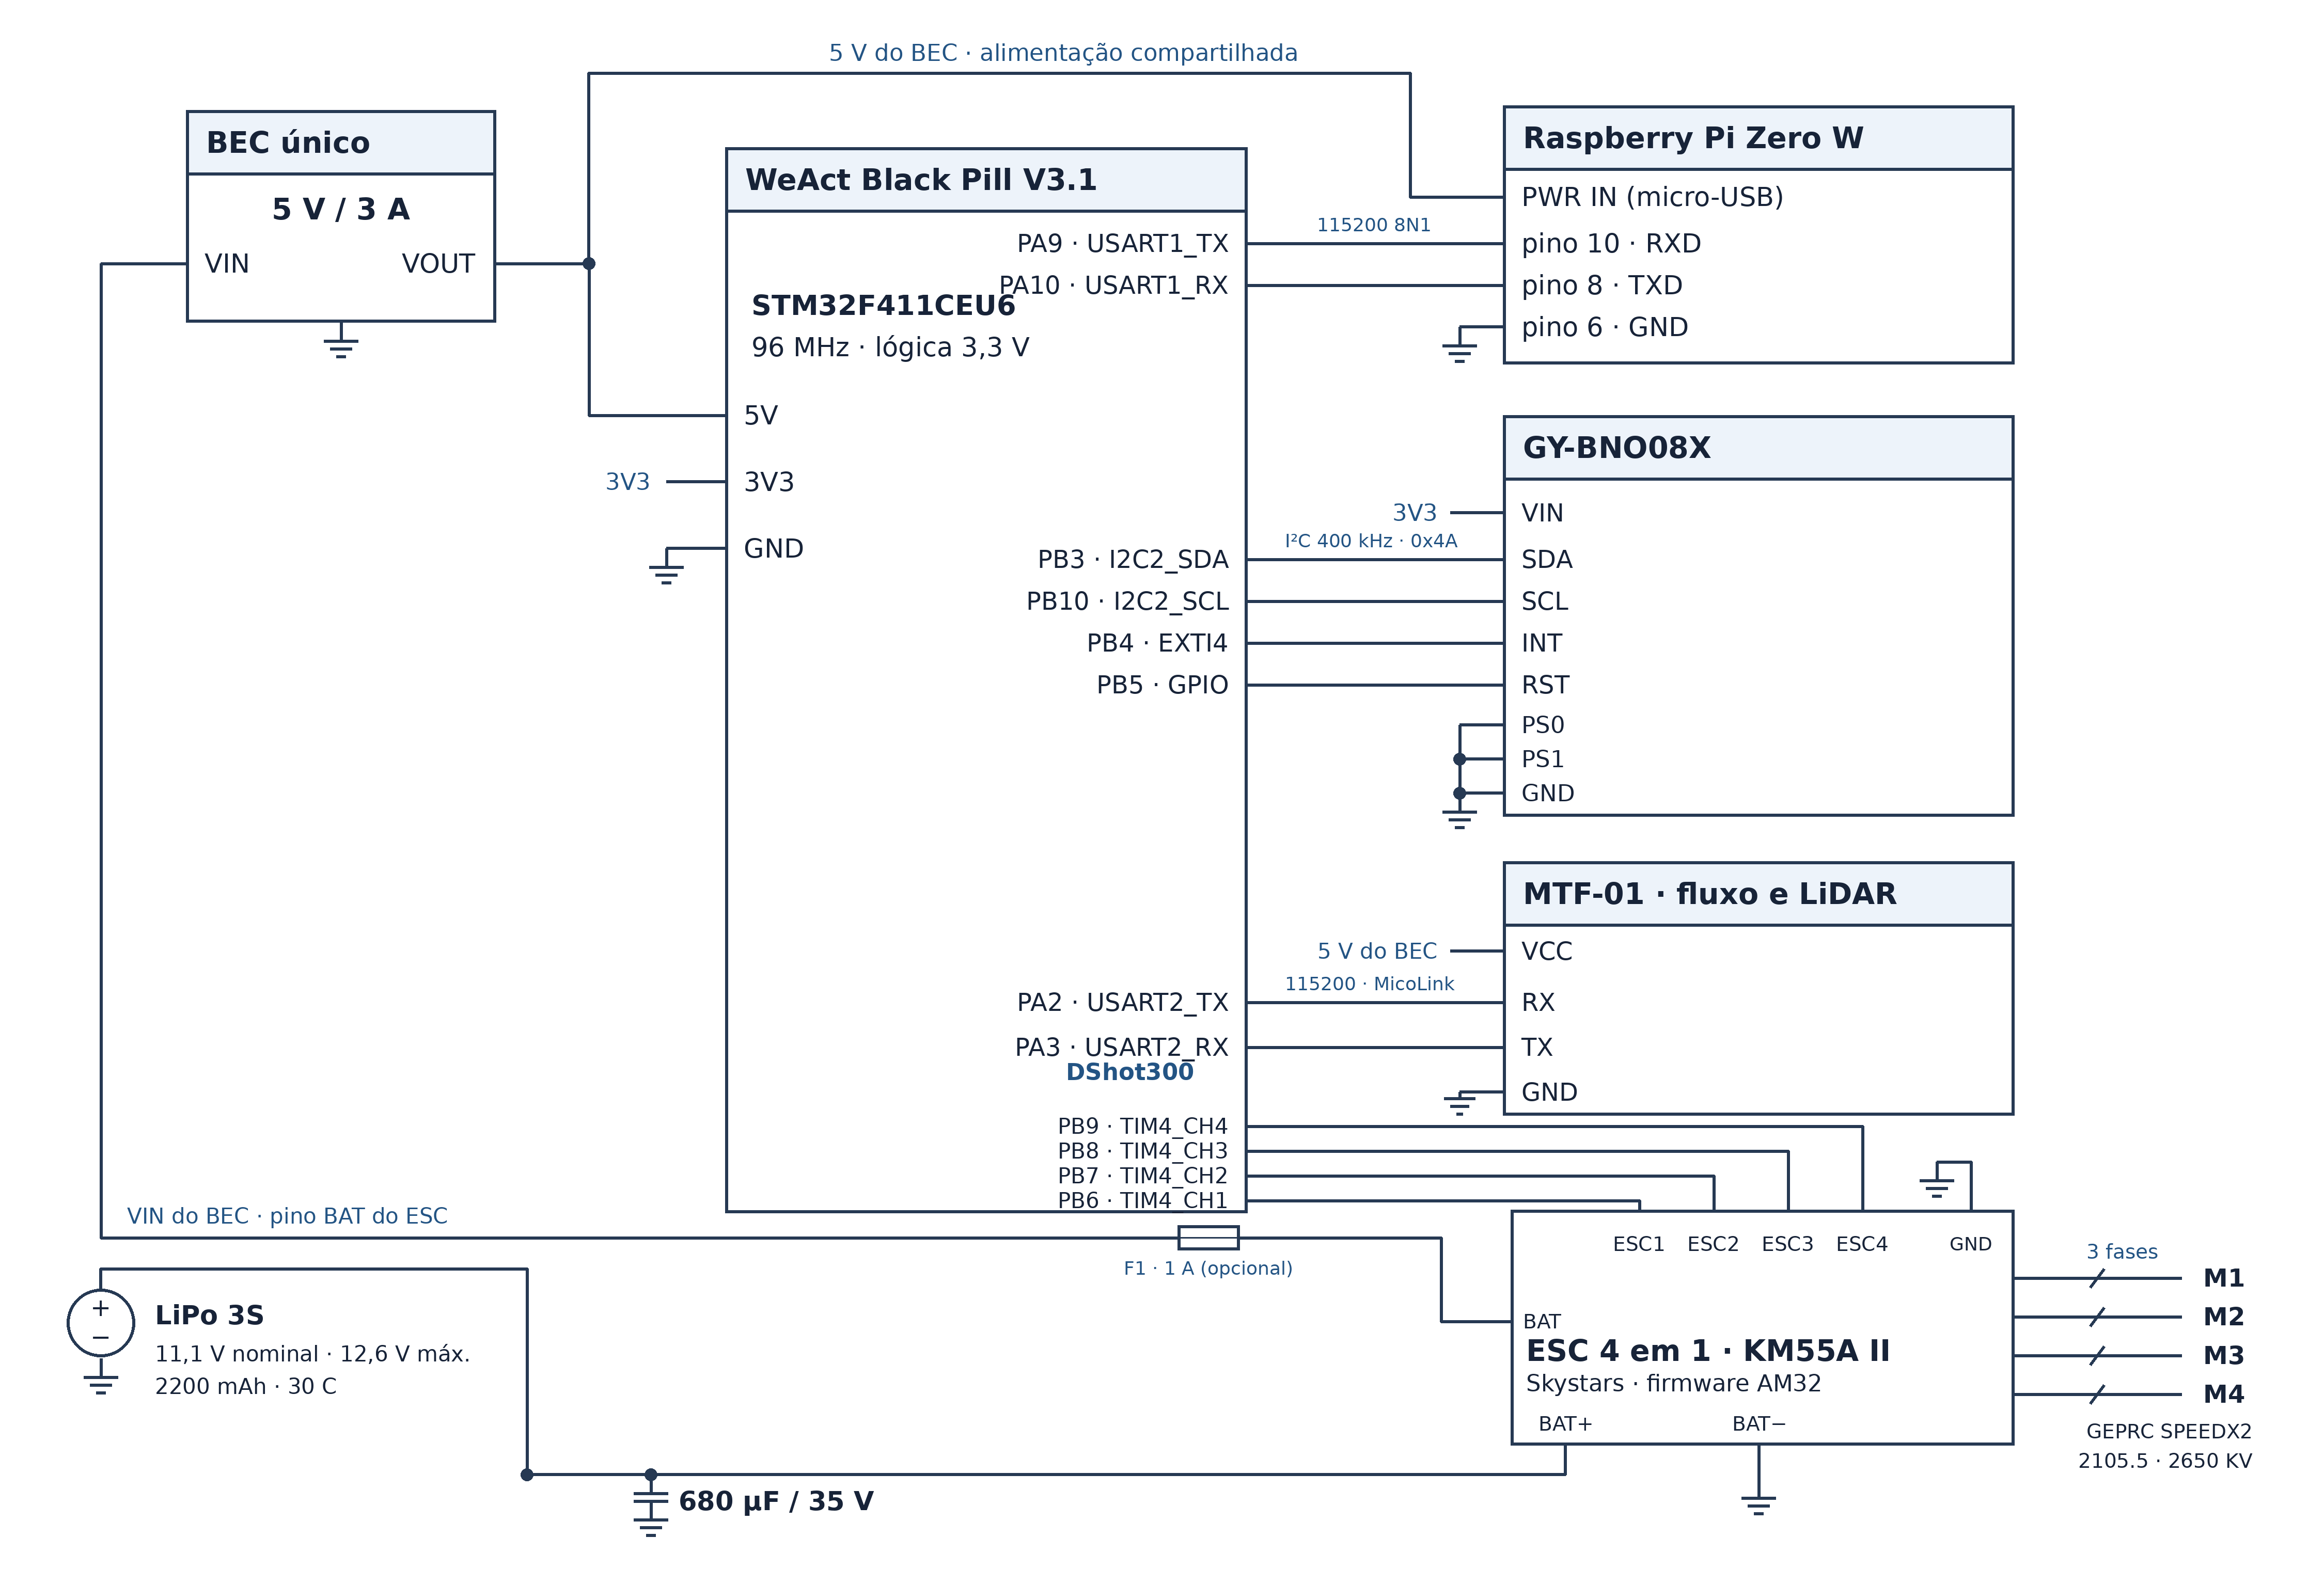
\includegraphics[width=\textwidth,height=0.85\textheight,keepaspectratio]{images/apendices/diagrama_eletrico.png}
        \par\vspace{0.2cm}
        \footnotesize Fonte: elaborado pelos autores (2026).
    \end{figure}
    \clearpage

    \addtocontents{toc}{\protect\setcounter{tocdepth}{0}}
\end{apendicesenv}

%\begin{anexosenv}

    \newpage
    \phantomsection
    
    \addcontentsline{toc}{chapter}{ANEXOS}
    \addtocontents{toc}{\protect\setcounter{tocdepth}{-1}}
    
    % coloca o primeiro anexo na mesma pagina do titulo do capitulo
    \chapter{Morbi ultrices rutrum lorem}
    \lipsum[30]

    \chapter{Cras non urna sed feugiat cum sociis natoque penatibus et magnis dis
    parturient montes nascetur ridiculus mus}
    \lipsum[31]

    \chapter{Fusce facilisis lacinia dui}
    \lipsum[32]
    
    \addtocontents{toc}{\protect\setcounter{tocdepth}{0}}
\end{anexosenv}

\printindex                     

\end{document}